%%%%%%%%%%%%%%%%%%%%%%%%%%%%%%%%%%%%%%%%%
% The Legrand Orange Book
% LaTeX Template
% Version 2.1.1 (14/07/16)
%
% This template has been downloaded from:
% http://www.LaTeXTemplates.com
%
% Mathias Legrand (legrand.mathias@gmail.com) with modifications by:
% Vel (vel@latextemplates.com)
% Alexander Wolf (alex.v.wolf@gmail.com)
% Georg Zotti (georg.zotti@univie.ac.at)
% Angelo Fraietta (a.fraietta@unsw.edu.au)
%
% License:
% CC BY-NC-SA 3.0 (http://creativecommons.org/licenses/by-nc-sa/3.0/)
%
% Compiling this template:
% This template uses biber for its bibliography and makeindex for its index.
% When you first open the template, compile it from the command line with the 
% commands below to make sure your LaTeX distribution is configured correctly:
%
% 1) pdflatex guide
% 2) makeindex guide.idx -s StyleInd.ist
% 3) biber guide
% 4) pdflatex guide x 2
%
% After this, when you wish to update the bibliography/index use the appropriate
% command above and make sure to compile with pdflatex several times 
% afterwards to propagate your changes to the document.
%
% This template also uses a number of packages which may need to be
% updated to the newest versions for the template to compile. It is strongly
% recommended you update your LaTeX distribution if you have any
% compilation errors.
%
% Important note:
% Chapter heading images should have a 2:1 width:height ratio,
% e.g. 920px width and 460px height.
%
%%%%%%%%%%%%%%%%%%%%%%%%%%%%%%%%%%%%%%%%%

%---------------------------------------------------------------------------------------
%   DETECT SWITCH FOR htlatex.
%---------------------------------------------------------------------------------------
% We can use package ifpdf to detect pdf creation. However, htlatex needs dvipdfmx in the document global options. 
% Therefore we need a new command (\ifhtlatex...\else...\fi) that even works before documentclass.

\newif\ifhtlatex
\ifx\HCode\UnDeFiNeD
  \htlatexfalse
\else
  \htlatextrue
\fi

%----------------------------------------------------------------------------------------
%	PACKAGES AND OTHER DOCUMENT CONFIGURATIONS
%----------------------------------------------------------------------------------------
\ifhtlatex
\documentclass[12pt,fleqn,dvipdfmx]{book} % Default font size and left-justified equations
\else
% There is still also demand of discerning latex from pdflatex at the documentclass line.
% http://tug.org/pipermail/macostex-archives/2006-January/020022.html
\ifx\pdfoutput\undefined
\documentclass[12pt,fleqn,dvipdfmx]{book} % Default font size and left-justified equations
\else
\documentclass[12pt,fleqn]{book} % Default font size and left-justified equations
\pdfcompresslevel=9
\fi
\fi
%----------------------------------------------------------------------------------------

\input{structure} % Insert the commands.tex file which contains the majority of the structure behind the template
\input{version}

\title{Stellarium User Guide}
\author{Georg Zotti \and Alexander Wolf (editors)}

%% GZ Some commands which can be used later, like version number etc.

\newcommand{\DocumentEdition}{1}

\begin{document}
\frontmatter
\VerbatimFootnotes % Allow \verb|whatever| in footnotes 

%----------------------------------------------------------------------------------------
%	TITLE PAGE
%----------------------------------------------------------------------------------------
\ifhtlatex
\maketitle
\else
\begingroup
\thispagestyle{empty}
\begin{tikzpicture}[remember picture,overlay]
\coordinate [below=12cm] (midpoint) at (current page.north);
\node at (current page.north west)
{\begin{tikzpicture}[remember picture,overlay]
\node[anchor=north west,inner sep=0pt] at (0,0) {\includegraphics[width=\paperwidth]{bookcover_cygnus.png}}; % Background image
\draw[anchor=north] (midpoint) node [fill=ocre!30!white,fill opacity=0.6,text opacity=1,inner sep=1cm]%
     {\Huge\centering\bfseries\sffamily\parbox[c][][t]{\paperwidth}%
                                              {\centering Stellarium \StelVersion\space User Guide\\[18pt] % Book title
                                              {\Large Georg Zotti, Alexander Wolf (editors)}\\[15pt]% Author names
                                              {\Large 2019}% Year
                                             }}; % 
\end{tikzpicture}};
\end{tikzpicture}
\vfill
\endgroup
\fi
%----------------------------------------------------------------------------------------
%	COPYRIGHT PAGE
%----------------------------------------------------------------------------------------

\newpage
~\vfill
\thispagestyle{empty}

\noindent Copyright \copyright\ 2014-\the\year{} Georg Zotti.\\        % Permanent copyright notice
\noindent Copyright \copyright\ 2011-\the\year{} Alexander Wolf.\\     % Permanent copyright notice
\noindent Copyright \copyright\ 2006-2013 Matthew Gates.\\             % Copyright notice
\noindent Copyright \copyright\ 2013-2014 Barry Gerdes (\dag\,2014).\\ % Copyright notice
\ifthenelse{\equal{\StelVersion}{0.15.0}}{%
\noindent \fbox{
  \begin{minipage}[t]{0.8\linewidth}
    Stellarium Version 0.15 is dedicated in memory of our team
    member Barry Gerdes (\dag\,2014).
  \end{minipage}
}\\}{}

\noindent%
\ifhtlatex
\url{https://stellarium.org}
\else
\textsc{stellarium.org}\\ % URL
\fi

\noindent Permission is granted to copy, distribute and/or modify 
this document under the terms of the GNU Free Documentation License, 
Version 1.3 or any later version published by the Free Software 
Foundation; with no Invariant Sections, no Front-Cover Texts, 
and no Back-Cover Texts. A copy of the license is included in 
the appendix~\ref{ch:License} entitled ``GNU Free Documentation
License''.\\ % License information

\small{\noindent \textit{All trademarks, third party brands, product names, trade names,
corporate names and company names mentioned may be trademarks of their
respective owners or registered trademarks of other companies and are
used for purposes of explanation and to the readers' benefit, without
implying a violation of copyright law.}}\\


\noindent \textit{Version \StelVersion-\DocumentEdition, \today} % Printing/edition date

%----------------------------------------------------------------------------------------
%	TABLE OF CONTENTS
%----------------------------------------------------------------------------------------

\chapterimage{chapter-t1-bg.png} % Table of contents heading image

\pagestyle{empty} % No headers
\ifpdf
 \tableofcontents % Print the table of contents itself
\fi
\cleardoublepage % Forces the first chapter to start on an odd page so it's on the right


\mainmatter
\pagestyle{fancy} % Print headers again
%% There should be one source file per chapter. 
%% Structural changes (chapter images etc.) should be in this main file to better have an overview.
%----------------------------------------------------------------------------------------
%	PART I
%----------------------------------------------------------------------------------------
\part{Basic Use}

%----------------------------------------------------------------------------------------
%	CHAPTER 1 (Introduction)
%----------------------------------------------------------------------------------------
\chapterimage{chapter-t2-bg.png} % Chapter heading image

\include{ch_introduction}

%% Activate this if you want to check the page layout.
%%\layout

%----------------------------------------------------------------------------------------
%	CHAPTER 2 (Installation)
%----------------------------------------------------------------------------------------
% \chapterimage{chapter-t2-bg.png} % Chapter heading image Did not change...

\include{ch_getting_started}

%----------------------------------------------------------------------------------------
%	CHAPTER 3 (was called Interface Guide, but is just a first tour.)
%----------------------------------------------------------------------------------------

\include{ch_tour}


%----------------------------------------------------------------------------------------
%	CHAPTER 4 (was called Configuration, but is really an in-depth description of the GUI panels.)
%----------------------------------------------------------------------------------------

% Status info:
% M. Gates	2006-2009
% A. Wolf	2011-2014
% B. Gerdes	2013
% Additions inserted from wiki 2015-12-26
% Content OK for 0.12.4.
% 2016-04 GZ started restructuring
% TODO: typo&grammar check

% \chapterimage{chapter-t2-bg} % Chapter heading image now set in guide.tex

\chapter{The User Interface}
\label{ch:gui}


This chapter describes the dialog windows which can be accessed from the left menu bar.

Most of Stellarium's settings can be changed using the view window
(press \guibutton[0.35]{2}{btd_view.png} or \key{F4}) and the
configuration window (\guibutton[0.35]{2}{btd_config.png} or
\key{F2}). Most settings have short labels. To learn more about some
settings, more information is available as \emph{tooltips}, small text
boxes which appear when you hover the mouse cursor over a
button.\footnote{Unfortunately, on Windows~7 and later, with some Nvidia
  and AMD GPUs in OpenGL mode, these tooltips sometimes do not work.}

You can drag the
windows around\newFeature{0.15}, and the position will be used again when you restart
Stellarium. If this would mean the window is off-screen (because you
start in windowed mode, or with a different screen), the window will
be moved so that at least a part is visible.

Some options are really rarely changed and therefore may only be
configured by editing the configuration file.  See
\ref{sec:ConfigurationFile} The Main Configuration File for more
details.



\section{Setting the Date and Time}
\label{sec:gui:date}

\begin{figure}[htbp]
\centering\includegraphics[width=0.75\textwidth]{date_and_time_dialog.png}
\caption{Date and Time dialog}
\label{fig:gui:date}
\end{figure}

In addition to the time rate control buttons on the main toolbar, you
can use the date and time window (open with the \guibutton[0.35]{2}{btd_time.png} 
button or \key{F5}) to set the simulation time. The values
for year, month, day, hour, minutes and seconds may be modified by
typing new values, by clicking the up and down arrows above and below
the values, and by using the mouse wheel.

The other tab in this window allows you to see or set
\indexterm{Julian Day} and/or \indexterm[Julian Day!Modified]{Modified Julian Day} numbers
(see~\ref{sec:Concepts:JulianDay}).

\section{Setting Your Location}
\label{sec:gui:location}

\begin{figure}[htbp]
\centering\includegraphics[width=0.85\textwidth]{location_dialog.png}
\caption{Location window}
\label{fig:gui:location}
\end{figure}

\noindent The positions of the stars in the sky is dependent on your location on
Earth (or other planet) as well as the time and date. For Stellarium to
show accurately what is (or will be/was) in the sky, you must tell it
where you are. You only need to do this once -- Stellarium can save your
location so you won't need to set it again until you move.

After installation\newFeature{0.13.1}, Stellarium uses an online service which tries to
find your approximate location based on the IP address you are
using. This seems very practical, but if you feel this causes privacy
issues, you may want to switch this feature off. You should also consider 
switching it off on a computer which does not move, to save network bandwidth.

To set your location more accurately, or if the lookup service fails,
press \key{F6} to open the location window (Fig.~\ref{fig:gui:location}). 
There are a few ways you can set your location:

\begin{enumerate}
\item Just click on the map.
\item Search for a city where you live using the search edit box at
  the top right of the window, and select the right city from the
  list.
\item Click on the map to filter the list of cities in the vicinity of
  your click, then choose from the shortlist.
\item Enter a new location using the longitude, latitude and other
  data.
\item Click on \menu{Get Location from GPS} if you have a GPS
  receiver. \newFeature{0.16/0.18.1} You activate a periodic request
  for GPS fixes. After a few seconds, the button should change color
  and give a textual feedback. Green indicates a good position, yellow
  indicates a 2D-fix only, which means altitudes are not
  available. (Leave the GPS device running for a few minutes and/or
  search a place with better sky view.) You could leave it running if
  you are operating a fast-moving observatory platform, but rather
  switch it off when you see a good fix, so that other programs can
  use the serial GPS connection.  Red signals an error, and further
  positions are not retrieved but the button is reset. You may press
  the button again to start over.

  Sometimes you have to try several times or let it run for a while to get a
  green button indicating a valid 3D fix including altitude.
  See section~\ref{sec:ExtraData:GPS} for configuration details.
\end{enumerate}

\noindent If you want to use the current location permanently, click on the
``use as default'' checkbox, disable ``Get location from Network'',
and close the location window.

Two settings may influence the landscape when changing locations:
\begin{description}
\item[Auto select landscapes] When changing the planet, 
a fitting landscape panorama will be shown when available. 
Also, \newFeature{23.2} when clicking on the earth map, 
a zero-altitude landscape is displayed in the approximate color of that location (taken from the map).
\item[Auto-enable atmosphere] When changing planet during
  location change, the atmosphere will be switched as required.
\end{description}

\subsection{Time Zones}
\label{sec:gui:location:timezones}
Locations in Stellarium's location database include their respective
time zone.\newFeature{0.15.1/0.19.0} When you click on a location in
the list, the time should be shown in the respective time zone.  If
daylight time rules exist and you have selected ``Enable daylight
saving time'', also this abomination of modern civilisation is respected. Most
users will require to have this setting active.

When you select ``Use custom time zone'', you can select other time zones.
Those that start with UTC have no daylight time rules.

Time zones were introduced in the 19th century, originally for
purposes of railway traffic synchronization. The first such action was
taken in 1847, and therefore Stellarium by default will present Local
Mean Solar Time (LMST) for dates before 1847, and ignore all
configured time zones unless you deliberately activate ``Use custom
time zone''. The history of time zones and their rules is very
complicated, though, and Stellarium should not be expected to find the
exact date when time zone use was introduced at a certain location or
country. Just be sure to use LMST when replaying historical
observations before the 20th century.

For even earlier observations, you can also set Local True Solar Time
(LTST), which is the time given by sundials. Here, 12 o'clock is the
time when the sun transits the meridian, strictly, daily. The
difference between LMST and LTST is called \emph{equation of time}. 
See section~\ref{sec:plugins:EquationOfTime} for more information.

When you click on the map to set your location, Stellarium has
currently no way to guess the timezone of the coordinate pair. In this
case, Local Mean Solar Time is presented, which only depends on
longitude and was the ``normal'' time before the development of time
zones. Either select a city from the list or manually select a time
zone.

\subsection{Geographical Regions}
\label{sec:gui:location:geographicalregions}

The world is split into political entities called ``countries''. \newFeature{0.21.2} 
Humans have an unappealing tendency of fighting over the question to which 
country some territories should be counted. Stellarium is an astronomy 
program which labels coordinates of locations like cities with a name. 
Earlier editions of Stellarium used countries as further superordinate 
entities to locations for identification purposes. In consequence to much 
unnecessary and unfriendly discussion we decided to completely drop the 
petty-minded assignment of political country names to locations in favour 
of geographical regions. There is only one known habitable planet, one 
humankind, and one sky. Stellarium users should overcome borders! 

For the ``region'' classification of sky cultures we use the same regions (see \ref{sec:skycultures:region}), 
and we follow the UN~M49 geoscheme\footnote{https://unstats.un.org/unsd/methodology/m49/} with extensions for other planets.

\subsection{Observers}
\label{sec:gui:location:observers}

In the list of Planets you can find entries called \emph{Solar System Observer}, \emph{Jupiter Observer} and 
similar for each major planet that has moons: Earth, Mars, Jupiter, Saturn, Uranus, and Neptune. 
These are specialized locations. When switching to them, you will find yourself looking 
onto the respective observed object (Sun, Jupiter, \ldots) from somewhat above the plane of the Solar system. 
By pressing \key{\Alt+\arrowkeyleft}/\key{\Alt+\arrowkeyright} you can rotate around a vertical axis through the observed object.
Likewise, by pressing \key{\Alt+\arrowkeyup}/\key{\Alt+\arrowkeydown} you can change the latitude of observation. Finally, 
with \key{\Alt+Home}/\key{\Alt+End} you can change the distance from the observed object. 


\section{The Configuration Window}
\label{sec:gui:configuration}

The configuration window contains general program settings, and many
other settings which do not concern specific display options. Press
the tool button \guibutton[0.35]{2}{btd_config.png} or \key{F2} to open.


\subsection{The Main Tab}
\label{sec:gui:configuration:main}


\begin{figure}[htbp]
\centering\includegraphics[width=0.75\textwidth]{config_dialog_main_tab.png}
\caption{Configuration Window: Main Tab}
\label{fig:gui:configuration:main}
\end{figure}

The Main tab in the configuration window (Fig.~\ref{fig:gui:configuration:main}) provides controls for
changing separately the program and sky culture languages.

The next setting group allows to enable using DE430/DE431 and DE440/DE441 ephemeris files. 
These files have to be installed separately. Most users do not require this. 
See section~\ref{sec:ExtraData:ephemerides} if you are interested.

The tab also provides the buttons for saving the current view direction as default 
for the next startup, and for saving the program configuration. 
Most display settings have to be explicitly stored to make a setting change permanent.

\subsection{The Information Tab}
\label{sec:gui:configuration:info}

\begin{figure}[htbp]
\centering\includegraphics[width=0.75\textwidth]{config_dialog_info_tab.png}
\caption{Configuration Window: Information Tab}
\label{fig:gui:configuration:info}
\end{figure}

The Information tab (Fig.~\ref{fig:gui:configuration:info}) allows you to set the type and amount of information
displayed about a selected object.
\begin{itemize}
\item Ticking or unticking the relevant boxes will control this.
\item The information displays in various colors depending on the type and
level of the stored data
\end{itemize}

\subsection{The Extras Tab}
\label{sec:gui:configuration:extras}

\begin{figure}[htbp]
\centering\includegraphics[width=0.75\textwidth]{config_dialog_extras_tab.png}
\caption{Configuration Window: Extras Tab}
\label{fig:gui:configuration:extras}
\end{figure}

The Extras tab (Fig.~\ref{fig:gui:configuration:extras}) allows you to
customize information displayed about a selected object, download more
star catalogs and also allows to hide or show additional buttons in
the lower button bar. 
\subsubsection{Customization of information displays}
The information display can be tweaked a bit with the options found in the GUI section ``Additional information settings''.

\subsubsection{Customization of button visibility on bottom toolbar}
If your screen is too narrow to show all buttons
or you simply don't need them because you prefer the keyboard shortcuts,
you can choose your optimal setup. The selection of buttons is stored immediately. 
\begin{description}
\item[Constellation boundaries] You can toggle display of constellation boundaries with this button.
\item[Asterism lines] You can toggle display of asterism lines with this button.
\item[Asterism labels] You can toggle display of asterism labels with this button.
\item[Ecliptic grid] You can toggle display of ecliptic coordinate grid with this button.
\item[ICRS grid] You can toggle display of the International Coordinate Reference System (equatorial J2000 coordinate grid) with this button.
\item[galactic grid] You can toggle display of galactic coordinate grid with this button.
\item[Cardinal points] You can toggle display of the ``Cardinal points'' button.
\item[Compass marks] You can toggle display of the ``Compass marks'' button.
\item[Night mode] You can toggle display of the nightmode button.
\item[Centering button] You can toggle display of the ``Center on selected object'' button.
\item[Fullscreen button] You can toggle display of the fullscreen button.
\item[Quit button] You can toggle display of the button to quit Stellarium.
\item[Nebula background] You can toggle display of DSO photographs with this button.
\item[Flip buttons] When enabled, two buttons will be added to
  the main tool bar which allow the main view to be mirrored in the
  vertical and horizontal directions. This is useful when observing
  through telecopes which may cause the image to be mirrored.
\item[DSS survey] You can toggle display of Digitized Sky Survey with this button (see section~\ref{sec:TOAST}).
\item[HiPS Surveys] You can toggle display of Hierarchical Progressive Surveys with this button (see section \ref{sec:gui:view:surveys}).
\item[Bookmarks] You can enable display of Bookmarks (Observing Lists) dialog with this button.
\item[Use buttons background] Applies a gray background under the buttons on the bottom bar.
\end{description}

\subsubsection{Download more star catalogs}
Stellarium comes with enough stars for casual stargazing with the
unaided eye or binoculars. If you have a telescope and want to see
more stars, here you can download more catalogs. (See Appendix~\ref{ch:Catalogues})

\subsection{The Time Tab}
\label{sec:gui:configuration:time}

\begin{figure}[htbp]
\centering\includegraphics[width=0.75\textwidth]{config_dialog_time_tab.png}
\caption{Configuration Window: Time Tab}
\label{fig:gui:configuration:time}
\end{figure}

The Time tab (Fig.~\ref{fig:gui:configuration:time}) allows to specify what simulation time should be used
when the program starts:

\begin{description}
\item[System date and time] Stellarium will start with
  the simulation time equal to the operating system clock.
\item[System date at] Stellarium will start with the
  same date as the operating system clock, but the time will be fixed at
  the specified value. This is a useful setting for those people who use
  Stellarium during the day to plan observing sessions for the upcoming
  evening.
\item[Other] some fixed time can be chosen which will
  be used every time Stellarium starts.
\end{description}

\noindent The middle field allows specify display formats for date and time on bottom toolbar:
\begin{description}
\item[JD] Stellarium will display Julian Days (JD).
\item[Date and time] Stellarium will display date and time in selected format.
\end{description}

\noindent The lowest field allows selection of the correction model for the time
correction $\Delta T$ (see section~\ref{sec:Concepts:DeltaT}). Default
is ``Modified Espenak and Meeus (2006)''. Please use other values only if you
know what you are doing.

\subsection{The Tools Tab}
\label{sec:gui:configuration:tools}

\begin{figure}[htbp]
\centering\includegraphics[width=0.75\textwidth]{config_dialog_tools_tab.png}
\caption{Configuration Window: Tools Tab}
\label{fig:gui:configuration:tools}
\end{figure}

The Tools tab (Fig.~\ref{fig:gui:configuration:tools}) contains planetarium options 
(like enabling/disabling of keyboard shortcuts for panning and zooming the main view) 
and options for screenshots.

\begin{description}
\item[Spheric mirror distortion] This option pre-warps the main view
  such that it may be projected onto a spherical mirror using a
  projector. The resulting image will be reflected up from the spherical
  mirror in such a way that it may shine onto a small planetarium
  dome (or even just the ceiling of your dining room), making a cheap planetarium projection system.
\item[Disc viewport] This option masks the main view
  producing the effect of a telescope eyepiece. It is also useful when
  projecting Stellarium's output with a fish-eye lens planetarium
  projector.
\item[Gravity labels] This option makes labels of objects in the
  main view align with the nearest horizon. This means that labels
  projected onto a dome are always aligned properly.
\item[Select single constellation] When active, clicking on a star
  that is member in the constellation lines will make the
  constellation stand out. See section~\ref{sec:starlore:singleConstellations} for details.
\item[Dithering] options to allow select better simulation of sky on different hardware.
\item[Auto zoom out returns to initial direction of view] When enabled,
  this option changes the behavior of the zoom out key
  \key{\textbackslash{}} so that it resets the initial direction of view in
  addition to the field of view.
\item[Enable keyboard navigation]
\item[Enable mouse navigation]
\item[Enable mouse zooming]
\item[Overwrite text color] --- enabling this option\newFeature{0.20.2} will ignore the 
  color settings for each celestial object and enable one color for text on the info panel 
  for all celestial objects. By default Stellarium uses white color for this option, 
  but you may re-define it through a color chooser\newFeature{0.20.3}.
\item[Set keyboard focus to day input] --- you may use this option to force setting the 
  keyboard focus on the day input field in the Date and Time dialog. 
  
  Important note: the focus in the sky will be lost when you open the 
  Date and Time dialog after enabling this option.
\item[Azimuth from South] Some users may be used to counting azimuth
  from south.
\item[Use decimal degrees] You can toggle usage of decimal degree format for coordinates.
\item[Topocentric coordinates] If you require planetocentric coordinates, you may switch this off. 
  Usually it should be enabled. (See~\ref{sec:Concepts:Parallax:Topocentric})
\item[Include nutation] Compute the slight wobble of earth's
  axis. This feature is active only about 500 years around J2000.0.
\item[Include aberration] Add effect of annual \indexterm{aberration of light} to the object's position (see \ref{sec:Concepts:Aberration}). 
     Note: This also influences the displayed position in the J2000 frame!
	 For didactic purposes you can exaggerate the effect by up to $5\times$. 
\item[Indication for mount mode] You can activate the short display of a message when switching type of used mount.
\item[Edit keyboard shortcuts\ldots] See section~\ref{sec:gui:help:hotkeys}.
\item[Mouse cursor timeout] You can decide whether, and when, the
  mouse cursor should disappear from view when not moved.
\item[Info text color at daylight] --- this is a color chooser\newFeature{0.20.3} for defining the 
  text color for the info panel at daylight to increase the contrast of the text. 
  By default Stellarium use black color.
\item[Use kinetic scrolling]  Text fields in \newFeature{0.18.3} 
dialogs can either be moved on sidebar handles (with this switch
disabled) or by dragging the text itself (enabled), as it is known
from touch-enabled devices like smartphones. 
\end{description}

\paragraph{Framerate intent} \label{sec:gui:configuration:tools:fps} The pace of screen updates (frames per second, FPS) depends on several factors: 
CPU speed, graphics card speed, screen size, number of displayed objects and grids, etc. 
As is common for interactive programs, the main program thread runs on a single core also on a multicore system. 
For running Stellarium, a CPU with few but fast cores will appear faster in total than a multicore system at slower CPU cycles.  
High-end systems may deliver needlessly high framerates, at cost of energy consumption.
The maximum FPS setting limits the frame rate when Stellarium is interactively operated 
(zoomed, panned, settings switched, etc.) 
After a few seconds, when Stellarium is not interactively operated, it falls back to a minimum FPS setting to conserve energy. 
Of course, when the system cannot even reach this FPS, the factual FPS will be lower and the system may be overloaded.
Keep in mind that the mimimum setting also applies to running scripts (non-interactively).

\paragraph{Font size and font selection} \newFeature{0.18.3} You can change the font sizes for on-screen
text and GUI dialogs separately.  For some purposes like presentations
it may be helpful to enlarge screen font size while keeping GUI font
regular, or vice versa.  It also depends on your screen size whether
all the object info fits on screen. This may also depend on the
writing system and installed font. If you are using a non-Western
character system and the default font looks bad, you can select
another system font. For this, edit \file{config.ini} (see
chapter~\ref{sec:Directories}): locate the \texttt{[gui]} section and
set the key \texttt{flag\_font\_selection=true}. On next start of
Stellarium, you will find two elements for font selection: one allows
you to pre-select a writing system, the other will then allow
selection of a font installed in your system that includes the
characters used in the selected writing system. When you have found
the best font, store your settings on the Main tab (see
section~\ref{sec:gui:configuration:main}) and you may edit
\file{config.ini} again to disable the font selection switches.

\paragraph{Screenshots} You can set the directory where screenshots
will be stored, and \newFeature{0.18.1} also whether you want
screenshots sized like Stellarium's window or some other, likely
larger size. The maximum possible size depends on your
hardware. $4096\times4096$ should be possible on most PCs, others may
even create $16384\times16384$ images. The vertical field of view will be the same as in the current view.

You can also set \newFeature{0.19.0} the file format. The exact selection depends on
platform and version of the underlying Qt framework. Notable formats are PNG (lossless), JPG (lossy),
JPEG (higher quality JPG), BMP (Windows Bitmap), WEBP, TIF (LZW compressed), TIFF (uncompressed),
PBM, PGM, PPM, XBM, XPM, and ICO (thumbnails).

Some printing workflows require particular DPI (dots per inch)
settings stored in the screenshots. \newFeature{0.22.0} You can
configure DPI which will be stored in the image metadata. The intended
print size in \mm\ is shown in the tooltip of the dpi spinner.

\subsection{The Scripts Tab}
\label{sec:gui:configuration:scripts}

\begin{figure}[htbp]
\centering\includegraphics[width=0.75\textwidth]{config_dialog_scripts_tab.png}
\caption{Configuration Window: Scripts Tab}
\label{fig:gui:configuration:scripts}
\end{figure}

The Scripts tab (Fig.~\ref{fig:gui:configuration:scripts}) allows the
selection of pre-assembled scripts bundled with Stellarium that can be
run (See chapter~\ref{ch:scripting} for an introduction to the
scripting capabilities and language). This list can be expanded with
your own scripts as required. See
section~\ref{sec:FilesAndDirectories:DirectoryStructure} where to
store your own scripts.

When a script is selected it can be run by pressing the arrow button
and stopped with the stop button. With some scripts the stop button is
inhibited until the script is finished. %% TODO: EXPLAIN HOW?

Scripts that use sound or embedded videos will need a version of
Stellarium configured at compile time with multimedia support
enabled. It must be pointed out here that sound or video codecs
available depends on the sound and video capabilities of you computer
platform and may not work.


\subsection{The Plugins Tab}
\label{sec:gui:configuration:plugins}

\begin{figure}[htbp]
\centering\includegraphics[width=0.75\textwidth]{config_dialog_plugins_tab.png}
\caption{Configuration Window: Plugins Tab}
\label{fig:gui:configuration:plugins}
\end{figure}


Plugins (see chapter~\ref{ch:Plugins} for an introduction) can be
enabled here (Fig.~\ref{fig:gui:configuration:plugins}) to be loaded the next time
you start Stellarium. When loaded, many plugins allow additional configuration
which is available by pressing the \menu{configure} button on this tab.


\section{The View Settings Window}
\label{sec:gui:view}

The View settings window controls many display features of Stellarium
which are not available via the main toolbar.

\subsection{The Sky Tab}
\label{sec:gui:view:sky}

\begin{figure}[htbp]
\centering\includegraphics[width=0.75\textwidth]{view_dialog_sky_tab.png}
\caption{View Settings Window: Sky Tab}
\label{fig:gui:view:sky}
\end{figure}

The Sky tab of the View window (Fig.~\ref{fig:gui:view:sky}) contains settings
for changing the general appearance of the main sky view and projections. Some highlights of sky field:
\begin{description}
\item[Dynamic eye adaptation] When enabled this feature reduces the
  brightness of faint objects when a bright object is in the field of
  view. This simulates how the eye can be dazzled by a bright object
  such as the moon, making it harder to see faint stars and galaxies.
\begin{samepage} % If the list of options is page-broken from the beginning of the "Light pollution" item, it becomes hard to orient in the text due to starting a page with a nested list.
\item[Light pollution] In urban and suburban areas, the sky is
  brightened by terrestrial light pollution reflected in the atmosphere.
  Stellarium simulates light pollution and lets the user configure how bright
  the night sky is.
  There are several ways to set it up:
  \begin{description}
    \item[Automatic from locations database] option makes Stellarium find sky
      brightness from its locations database and simulate light pollution
      without any further user input.
    \item[Manual] mode lets the user choose the amount of light pollution by
      moving a slider. To make it easier to orient in the resulting amount of
      light pollution, a tooltip will show the classification of the sky
      according to the \emph{Bortle Dark Sky Scale} (See Appendix~\ref{ch:BortleScale}
      for more information), as well as the naked-eye limiting magnitude.
    \item[Manual from SQM] mode lets one enter the reading of a \emph{Sky Quality Meter}.
      Stellarium can accept it in several units: physical ($\mathrm{cd/m^2}$,
      $\mathrm{mcd/m^2}$, $\mathrm{\mu cd/m^2}$) as well as astronomical,
      $\mathrm{mag/arcsec^2}$. To enter a value, first choose the unit, and
      then type the number into the spinbox.
  \end{description}
\end{samepage}
\item[Solar altitude for Twilight Finder] You can configure \newFeature{0.21.2} 
shortcut keys to go to the time when the sun reaches this altitude below the 
mathematical horizon. See section~\ref{sec:gui:help:hotkeys:example}.
\item[Shooting stars] Stellarium has a simple meteor simulation
  option. This setting controls how many shooting stars will be shown.
  Note that shooting stars are only visible when the time rate is 1, and
  might not be visible at some times of the day. Meteor showers can be
  simulated using a dedicated plugin (see section~\ref{sec:plugins:MeteorShowers}).
\end{description}

\noindent Some highlights of the stars field:
\begin{description}
\item[Absolute scale] is the size of stars as rendered by
  Stellarium. If you increase this value, all stars will appear larger
  than before.
\item[Relative scale] determines the difference in size of bright
  stars compared to faint stars. Values higher than 1.00 will make the
  brightest stars appear much larger than they do in the sky. This is
  useful for creating star charts, or when learning the basic
  constellations.
\item[Twinkle] controls how much the stars twinkle when atmosphere is
  enabled (\indexterm{scintillation}, see section~\ref{sec:phenomena:Scintillation}). 
  Since v0.15.0, the twinkling is reduced in higher altitudes,
  where the star light passes the atmosphere in a steeper angle and is
  less distorted.
\item[Limit magnitude] Inhibits automatic addition of fainter stars
  when zooming in. This may be helpful if you are interested in naked
  eye stars only.
\item[Labels and markers] you can independently change the amount of
  labels displayed for stars. The further to the
  right the sliders are set, the more labels you will see. Note that
  more labels will also appear as you zoom in.
\item[Use designations for screen labels] --- when this option is
  enabled you will see in the sky (on-screen labels) only scientific
  designations (catalog numbers) of the stars instead of their common
  names. To customize\newFeature{0.21.3} the on-screen labels we
  added 3 additional options\footnote{These options are only used if the 
  star does not have Bayer/Flamsted designations.}
 --- \textbf{Dbl. stars}, \textbf{Var. stars} and \textbf{HIP} --- which will show, 
  in this sequence of preference, the first available occurrence of 
  the traditional designations of double stars, 
  variable stars or HIP numbers, respectively. 
\end{description}

\subsubsection{The Projections field}
\label{sec:gui:view:sky:projections}

Selecting items in this list changes the
  projection method which Stellarium uses to draw the sky~\citep{Snyder:MapProjections}. Options are:

\begin{description}
  \item[Perspective] Perspective projection maps the horizon and other
    great circles like equator, ecliptic, hour lines, etc. into
    straight lines. The maximum field of view is 150\degree. The
    mathematical name for this projection method is \emph{gnomonic
      projection}.
  \item[Stereographic] Stereographic projection has been known since
    antiquity and was originally known as the planisphere
    projection. It preserves the angles at which curves cross each
    other but it does not preserve area. Else it is similar to
    fish-eye projection mode. The maximum field of view in this mode
    is 235\degree.
  \item[Fish-Eye] Stellarium draws the sky using \emph{azimuthal
    equidistant projection}. In fish-eye projection, straight lines
    become curves when they appear a large angular distance from the
    center of the field of view (like the distortions seen with very
    wide angle camera lenses). This is more pronounced as the user zooms
    out. The maximum field of view in this mode is 180\degree.
  \item[Orthographic] Orthographic projection is related to
    perspective projection, but the \emph{point of perspective} is set
    to an infinite distance. The maximum field of view is 180\degree.
  \item[Equal Area] The full name of this projection method is
    \emph{Lambert azimuthal equal-area projection}. It preserves the
    area but not the angle. The maximum field of view is 360\degree.
  \item[Hammer-Aitoff] The Hammer projection is an equal-area map
    projection, described by \name[Ernst von]{Hammer} (1858--1925) in 1892 and directly inspired
    by the Aitoff projection. The maximum field of view in this mode is
    360\degree.
  \item[Sinusoidal] The sinusoidal projection is a
    \emph{pseudocylindrical equal-area map projection}, sometimes
    called the Sanson--Flamsteed or the Mercator equal-area
    projection. Meridians are mapped to sine curves.
  \item[Mercator] Mercator projection is a cylindrical projection developed 
    by \name[Gerardus]{Mercator} (1512--1594)
    which preserves the angles between objects, and the scale around
    an object is the same in all directions. The poles are mapped to
    infinity.  The maximum field of view in this mode is 233\degree.
  \item[Miller cylindrical] The Miller cylindrical projection is a
    modified Mercator projection, proposed by \name[Osborn Maitland]{Miller}
    (1897--1979) in 1942. The poles are no longer mapped to
    infinity.
  \item[Cylinder] The full name of this simple projection mode is
    \emph{cylindrical equidistant projection} or \emph{Plate
      Carr\'ee}. The maximum field of view in this mode is 233\degree.
\end{description}

\noindent Two more settings allow finetuning:
\begin{description}
\item[Vertical viewport offset] If you have a wide screen or like wide-angle views,
you may feel that too much of screen space lies below the horizon. This setting can shift the view up or down.
\item[Custom FoV limit] Some projections allow very wide views, like 180°
which covers a complete \newFeature{0.21.2} celestial hemisphere (e.g.\ the entire skydome)
or even more. In some cases like if you are running a planetarium, you may want
to limit the vertical field of view so that you won't ever zoom out too far.
\end{description}

\subsubsection{Atmosphere settings}
\label{sec:gui:view:sky:atmosphere}

An auxiliary dialog opens when you select \guibutton[1.0]{0.75}{uibtSettings.png}
and contains detail settings for the atmosphere. Here
you can choose visual model of atmosphere, set atmospheric pressure and temperature which influence
refraction (see section~\ref{sec:phenomena:Refraction}) and the
opacity factor $k_v$ for extinction, \emph{magnitude loss per airmass} 
(see section~\ref{sec:phenomena:Extinction}).

There are two visual models for the atmosphere available:
\begin{description}
  \item[Preetham] This is the legacy model (see section~\ref{sec:skylight:Preetham}), fallback for the cases
    when the other one doesn't work.
  \item[ShowMySky] This model is the more realistic visual model of
    the atmosphere colors (see section~\ref{sec:skylight:ShowMySky}). It
    relies on a precomputed dataset that can be chosen in the user
    interface after the \program{ShowMySky} model is enabled.
\end{description}

\subsection{The Solar System Objects (SSO) Tab}
\label{sec:gui:view:sso}

The Solar System Objects tab of the View window (Fig.~\ref{fig:gui:view:sso}) contains settings
for changing the general appearance of the view of Solar system objects. Some highlights:

\begin{figure}[htbp]
\centering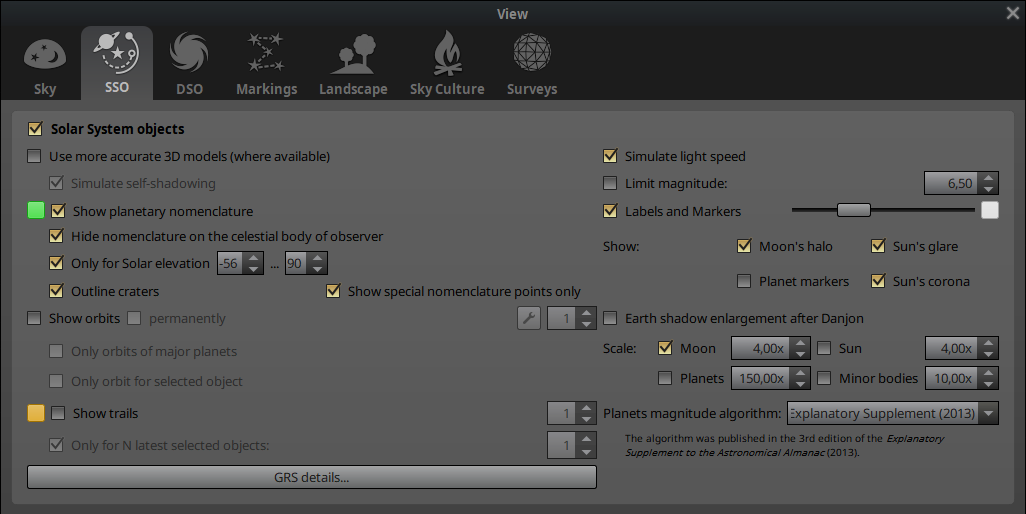
\includegraphics[width=0.75\textwidth]{view_dialog_sso_tab.png}
\caption{View Settings Window: SSO Tab}
\label{fig:gui:view:sso}
\end{figure}


\begin{description}
\item[Simulate light speed] will give more precise positions for planetary bodies which move
  rapidly against background stars (e.g. the moons of Jupiter).
\item[Scale] will increase the apparent size of the selected class of objects:
  \begin{description}
  \item[Moon] will increase the apparent size of the Moon
  in the sky, which can be nice for wide field of view shots.
  \item[Minor bodies] will increase the apparent size of minor
  bodies: planet satellites, all kinds of asteroids, and comets.  
  Forsome of these 3D models are available, which will be better
  discernible if enlarged.
  \item[Sun] will increase the apparent size of the Sun
    in the sky, which can be nice for didactic purposes or demonstrations.
  \item[Planets] will increase the apparent size of major planets.
  \end{description}
\item[Show orbits] adds a rendition of the orbit or trajectory of an SSO. 
For efficiency, orbits are not displayed when the object is not inside the screen, 
unless you set the ``permanently'' option. You can further fine-tune the selection 
and appearance (width and colors) of orbits with the additional settings. 
\item[Show trails] plots the apparent path of SSO among the stars as
  seen from the current planet.
\item[Show planetary nomenclature] displays positions and names of
  surface features officially named by the IAU (See
  Appendix~\ref{ch:Nomenclature}). When the sun is below the horizon
  at the location of the feature, the label is attenuated. A few special markers 
  show Centre, North and South poles, east and west points along the equator, 
  and the subsolar point (where the sun is at the zenith as seen from that feature). 
  Features like craters are best visible when they are illuminated by a low sun. 
  You can therefore limit the display\newFeature{1.2} to items along the
  \indexterm{terminator} (the border between light and dark on the surface).
  You can also\newFeature{23.3} mark craters and lunar \emph{maria} (the dark ``seas'') with circles. 
\item[GRS details\ldots]: The Great Red Spot (GRS) is slowly
  drifting along Jupiter's System~II coordinate system. This button 
  opens a new dialog in which you can adjust the longitude (Jupiter system~II) 
  and annual drift rate of this feature at a particular epoch. To help you,
  another button in this dialog opens a website with relevant data.
  The central meridian data given
  \newFeature{0.21.0} in the object information on screen still shows
  System~II longitude.
\item[Labels and markers] you can independently change the amount of
  labels displayed for Solar system objects. The further to the
  right the sliders are set, the more labels you will see. Note that
  more labels will also appear as you zoom in.
\item[Planet magnitude algorithm] several ways to compute planet
  magnitudes have been made available from the literature. Data by
  Müller (1893) provide visual magnitudes. The other models provide
  instrumental (Johnson V) magnitudes.
\item[Earth shadow enlargement after Danjon] \newFeature{0.21.0}
  Earth's shadow is enlarged by the atmosphere. You can select whether
  the 2\% enlargement used by the Astronomical Almanac should be
  applied (default), or the formulation of \name{Danjon}
  (see section~\ref{sec:Eclipses:lunar}).
\end{description}

% Put these 3 on 1 page.
\begin{figure}[p]
\centering\includegraphics[width=0.75\textwidth]{view_dialog_dso_tab.png}
\caption{View Settings Window: DSO Tab}
\label{fig:gui:view:dso}
\end{figure}

\begin{figure}[p]
\centering\includegraphics[width=0.75\textwidth]{view_dialog_markings_tab.jpg}
\caption{View Settings Window: Markings Tab}
\label{fig:gui:view:markings}
\end{figure}

\begin{figure}[p]
\centering\includegraphics[width=0.75\textwidth]{view_dialog_landscape_tab.png}
\caption{View Settings Window: Landscape Tab}
\label{fig:gui:view:landscape}
\end{figure}

\subsection{The Deep-Sky Objects (DSO) Tab}
\label{sec:gui:view:dso}

\indexterm{Deep-sky objects} or DSO are extended objects which are
external to the solar system, and are not point sources like stars.
DSO include galaxies, planetary nebulae and star clusters. These
objects may or may not have images associated with them. Stellarium
comes with a catalog of over 90,000 extended objects containing
the combined data from many catalogs, with 500+ images.  

The DSO tab (Fig.~\ref{fig:gui:view:dso}) allows you to specify which 
catalogs or which object types you are interested in. This selection 
will also be respected in other parts of the program, 
most notably Search (section~\ref{sec:gui:search}) and 
AstroCalc/WUT (section~\ref{sec:gui:AstroCalc:WUT}) 
will not find objects from catalogs which you have not selected here. 

See chapter~\ref{ch:DSO} for details about the catalog, 
and how to extend it with your own photographs.


\subsection{The Markings Tab}
\label{sec:gui:view:markings}

\noindent The Markings tab of the View window
(Fig.~\ref{fig:gui:view:markings}) controls plotting various grids and
lines on the celestial sphere. Colors for grids, lines and points can be
adjusted by clicking on the corresponding colored square.  The central
column governs lines like equator, ecliptic, meridian etc., where each
can optionally be fine-tuned to \newFeature{0.20.0} show partition
marks and labels. Color settings are stored immediately, all other
flags need explicit saving of the settings (see section
\ref{sec:gui:configuration:main}).

\subsection{The Landscape Tab}
\label{sec:gui:view:landscape}

The Landscape tab of the View window
(Fig.~\ref{fig:gui:view:landscape}) controls the landscape graphics
(the horizon which surrounds you). To change the landscape graphics,
select a landscape from the list on the left side of the window. A
description of the landscape will be shown on the right.

Note that while a landscape  can include information about where the
landscape graphics were taken (planet, longitude, latitude and
altitude), this location does not have to be the same as the location
selected in the Location window, although you can set up Stellarium such
that selection of a new landscape will alter the location for you.

The controls at the bottom right of the window operate as follows:

\begin{description}
\item[Use this landscape as default] Selecting this option will save
  the landscape into the program configuration file so that the current
  landscape will be the one used when Stellarium starts.
\item[Show ground] This turns on and off landscape rendering (same
  as the button \guibutton{0.6}{bt_ground.png} in the main tool bar).
\item[Show fog] This turns on and off rendering of a band of
  fog/haze along the horizon, when available in this landscape.
\item[Show illumination] to reflect the ugly developments of our
  civilisation, landscapes can be configured with a layer of light
  pollution, e.g., streetlamps, bright windows, or the sky glow of a
  nearby city. This layer, if present, will be mixed in when it is
  dark enough.
\item[Show landscape labels] Landscapes can be configured with a
  gazetteer of interesting points, e.g., mountain peaks, which can be
  labeled with this option. Color and font size can also be configured.
\item[Position from landscape] When enabled, selecting a
  new landscape will automatically update the observer location.
  Use this if the landscape is not just decoration, but a true
  representation of a particular site you wish to visit in the simulation.
\item[Minimal brightness] Moonless night on very dark locations may appear too dark
  on your screen. You may want to configure some minimal brightness here.
  \begin{description}
\item[from landscape, if given] Landscape authors may decide to
  provide such a minimal brightness value in the \file{landscape.ini}
  file. 
  \end{description}
\item[Draw only polygon]\newFeature{0.20.2} If a polygonal horizon line has been
  defined for the landscape, only draw this with the given thickness.
\item[Transparency] Allow peeking below the horizon. \newFeature{23.3} Note that this may show graphical errors. 
\end{description}

\noindent Using the button \menu{Add/remove landscapes\ldots}, you can also
install new landscapes from ZIP files which you can download e.g.\
from the Stellarium
website\footnote{\url{https://stellarium.org/landscapes.html}}
or create yourself (see ch.~\ref{ch:landscapes} Landscapes), or remove
these custom landscapes.

Loading large landscapes may take several seconds. \newFeature{0.15.2}
If you like to switch rapidly between several landscapes and have enough memory, 
you can increase the default cache size to keep more landscapes loaded previously 
available in memory. Note that a large landscape can take up 200MB or more! 
See section \ref{sec:configini:landscape}.

\subsection{The Starlore Tab}
\label{sec:gui:view:starlore}


\begin{figure}[th]\centering
\includegraphics[width=\textwidth]{stellarium-skycultures-map.jpg}
\caption{World map showing Stellarium's built-in set of
  sky cultures. To avoid overcrowding, smaller European sky cultures
  which are mostly derivatives or relatives of the ``Modern'' sky culture are not
  shown. (Image: S. M. Hoffmann)}
\label{fig:skycultures}
\end{figure}

\noindent If you want to explore humankind's cultural history, you could also
switch to the viewpoint of other ancient or contemporary
people. Constellations are defined as patterns in the sky serving to
set calendar marks and to navigate while travelling on Earth. Which
patterns are seen depends on the natural environment and the cultural
habits of the people, i.e., the Inuit in the arctic area might have
seen an Elk where the Chinese have seen a huge spoon or dipper. There
cannot be any astrological influence from these patterns as they had
been seen differently and, thus, are a product of human's
imagination. So, pointing out these cultural differences might have an
educational function, too.

\noindent%
\colorbox{light-gray}{\fbox{\parbox[t]{0.975\linewidth}{
\paragraph{Caution} Some of our native peoples' constellations are contributed for noncommercial use only.
Please respect their heritage holders and check-out the CC licence
version in the description before you use sky cultures for
broadcasting! See section~\ref{sec:skycultures:licenses} for details.}}}


\begin{figure}[htbp]
\centering\includegraphics[width=0.75\textwidth]{view_dialog_starlore_tab.png}
\caption{View Settings Window: Starlore Tab}
\label{fig:gui:view:starlore}
\end{figure}

The Starlore tab of the View window (Fig.~\ref{fig:gui:view:starlore})
controls which culture's constellations and bright star names will be
used in the main display.  Some cultures have constellation art (e.g.,
Western and Inuit), and the rest do not. Configurable options include
\begin{description}
\item[Use this sky culture as default] Activate this option to load
  this sky culture when Stellarium starts.
\item[Show labels] Activate display of constellation labels, like
  \guibutton{0.6}{bt_constellation_name.png} or \keys{V}. You can further
  select whether you want to display abbreviated, original or
  translated names.
\item[Show lines with thickness\ldots] Activate display of stick
  figures, like \guibutton{0.6}{bt_constellation.png} or \keys{C}, and you
  can configure constellation line thickness here.
\item[Show asterism lines\ldots] Activate display of asterism stick figures   
  (like the shortcut \keys{Alt+A}), and you can configure asterism line thickness here.\newFeature{0.16.0}
\item[Show ray helpers\ldots] Activate display of special navigational lines which 
  connect stars often from different constellations (like the shortcut \keys{Alt+R}),
  and you can configure thickness of those lines here.\newFeature{0.17.0}
\item[Show boundaries] Activate display of constellation boundaries,
  like \keys{B}. Currently, boundaries have been defined only for
  ``Modern'' sky cultures.
\item[Use native names for planets] If provided, show the planet names
  as used in this sky culture (also shows modern planet name for
  reference). %% TODO THIS FEATURE NEEDS SOME REWORK!
\item[Show art in brightness\ldots] Activate display of constellation
  art (if available), like \guibutton{0.6}{bt_constellation_art.png} or
  \keys{R}. You can also select the brightness here.
\item[Show asterism labels] Activate display of asterism labels, like \keys{Alt+V}.\newFeature{0.16.0}
\end{description}

\subsubsection{Select single constellations}
\label{sec:starlore:singleConstellations}

Some presenters may want to explain a particular storyline about the
constellations of a sky culture, which includes showing single
constellations or showing a sequence of appearing constellations. To
achieve this, first activate the single constellation mode (see
section~\ref{fig:gui:configuration:tools}).  Then, click on a star
which is part of a constellation line set. Click
another star which is part of another constellation to show that one.

If you explain a sky culture where constellations also have borders
defined, a click anywhere in the constellation area is enough.  For
other sky cultures, clicking onto a star which is not member of a
constellation line will display all constellations.

Press \keys{W} to remove all but the last selected constellation.
If you had deleted selection (right mouse click) before pressing \keys{W},
all constellations are hidden.
Press \keys{W} again to also hide the single displayed one, or click
another star to select the next constellation. If you need to keep the
single constellation visible, select the currently selected star again
to select it again.  Press \keys{Alt+W} to show all constellations.

With a little training, you will be able to give inspiring
constellation tours.

\subsection{The Surveys Tab}
\label{sec:gui:view:surveys}

\begin{figure}[htbp]
\centering\includegraphics[width=0.75\textwidth]{view_dialog_surveys_tab.png}
\caption{View Settings Window: Surveys Tab}
\label{fig:gui:view:surveys}
\end{figure}

The Surveys tab\newFeature{0.18.0} (Fig.~\ref{fig:gui:view:surveys}) allows to toggle the
visibility of online sky or solar system surveys (see chapter~\ref{ch:surveys}
for description of the surveys format).  Currently, only HiPS surveys are
supported.

On the left side of the window we see the list of available surveys from
the configured sources (See section \ref{sec:config.ini:hips} for how to
change the default sources).  On the right side a description of the selected
survey and its properties are displayed.

Surveys are grouped by types. The top combobox allows to filter the listed
surveys according to a given type (Deep Sky or Solar System).

You can toggle the visibility of a survey by checking the box on the left
of the survey name in the list.  (Note that as of v0.18.0, only a single deep
sky survey can be rendered at a time, so it makes no sense to select more than one in
the list!) Once a survey is visible you should be able to see its loading
status in the loading bar area of the sky view.

Deep sky surveys will be rendered aligned with the sky view, while solar system
surveys automatically map on the proper body.


\section{The Search Window}
\label{sec:gui:search}

\begin{figure}[p]
\centering\includegraphics[width=0.68\textwidth]{search_dialog.png}
\caption{The Search Window: Object}
\label{fig:gui:search}
\end{figure}

\begin{figure}[p]
\centering\includegraphics[width=0.68\textwidth]{search_dialog_recent_result.png}
\caption{The Search Window: Object (Recent Searches)}
\label{fig:gui:search:recentSearches}
\end{figure}

\begin{figure}[p]
\centering\includegraphics[width=0.68\textwidth,trim=0 30 0 0,clip]{search_dialog_simbad.png}
\caption{The Search Window: SIMBAD}
\label{fig:gui:search:simbad}
\end{figure}

\begin{figure}[p]
\centering\includegraphics[width=0.68\textwidth,trim=0 40 0 0,clip]{search_dialog_position.png}
\caption{The Search Window: Position}
\label{fig:gui:search:position}
\end{figure}

\begin{figure}[tbp]
\centering\includegraphics[width=0.68\textwidth]{search_dialog_list.png}
\caption{The Search Window: Lists}
\label{fig:gui:search:lists}
\end{figure}


\begin{figure}[tbp]
\centering\includegraphics[width=0.68\textwidth]{search_dialog_option.png}
\caption{The Search Window: Options}
\label{fig:gui:search:options}
\end{figure}

\subsection{The Object tab}
\label{sec:gui:SearchWindow:Object}
The Object tab of the Search window provides a convenient way to locate objects
in the sky. Simply type in the name of an object to find, and press
\key{\return}. Stellarium will point you at that object in the sky.

As you type, Stellarium will make a list of objects which contains 
what you have typed so far. The first of the list of matching objects
will be highlighted. If you press the \key{\tab} or \key{\arrowkeydown} key,
the selection will change to the next item in the list.
Pressing the \key{\arrowkeyup} key will bring you to the previous item.
Hitting the \key{\return} key will center on the
currently highlighted object and close the Search window.

For example, suppose we want to locate Saturn's moon Mimas (SI).
Open the Search window (\guibutton[0.5]{2.5}{btd_find.png}, \key{F3}, or \key{Ctrl+F}).
Type the first letter of the name, \emph{m}, to see a list
of objects whose name contains \emph{m}:
\begin{center}
\begin{tabular}{l}
        \emph{M}iranda (UV)\\
        Psa\emph{m}athe (NX)\\
        U\emph{m}briel (UII)\\
        \ldots\\
\end{tabular}
\end{center}

\noindent You may want at this point to have Stellarium rather propose object
names which start with the string you enter. Do that in the Options tab
of this panel (see section~\ref{sec:gui:SearchWindow:Options}).
The search result should update automatically\newFeature{0.20.3}
when you nagivate back to the Object tab.
Now the list is shorter and contains only objects which start
with \emph{m}:
\begin{center}
\begin{tabular}{l}
        \emph{M}ago\\
        \emph{M}aia\\
        \emph{M}ars\\
        \ldots\\
\end{tabular}
\end{center}

\noindent The first item in this list, Mago, is
highlighted. Pressing \key{\return} now would go to Mago, but we want
Mimas (SI). We can either press \key{\tab} or \key{\arrowkeydown} a few times to highlight Mimas (SI)
and then hit \key{\return}, or we can continue to type the name until
it is the first/only object in the list.

After you searched for an object, the next time the Search window opens,\newFeature{0.20.3}
your most recently searched object(s)
will automatically appear in the search result of the Object tab.
For instance, continuing with our example, re-open the Search window's Object tab.
Mimas (SI) should already be populated and highlighted:
\begin{center}
\begin{tabular}{l}
        \textbf{\emph{M}imas (SI)}\\
\end{tabular}
\end{center}

\noindent The Object tab's search result will now prioritize your most recent searches
(which will be shown in \textbf{bold}).\newFeature{0.20.3}
To modify the search results, see section~\ref{sec:gui:SearchWindow:Options}.
From our earlier example, re-enter \emph{m} into the Object tab.
Doing so will generate a slightly different list than before.
In this case, Mimas (SI) will appear first, as shown in Figure~\ref{fig:gui:search:recentSearches}:
\begin{center}
\begin{tabular}{l}
        \textbf{\emph{M}imas (SI)}\\
        \emph{M}ago\\
        \emph{M}aia\\
        \emph{M}ars\\
        \ldots\\
\end{tabular}
\end{center}

\subsection{The SIMBAD tab}
\label{sec:gui:SearchWindow:SIMBAD}
The SIMBAD tab (Fig.~\ref{fig:gui:search:simbad}) provides a
convenient way to fetch and show a set of information for selected
object from the astronomical online database
SIMBAD~\citep{2000A&AS..143....9W}.  If some object is only visible in
a survey or DSS background (see section~\ref{ch:surveys}) and not in
Stellarium's catalogs, you can also set a custom marker (see
section~\ref{sec:tour:markers}), select it and query SIMBAD ``tell me
what's known about objects at this location''.

\subsection{The Position tab}
\label{sec:gui:SearchWindow:Position}
The Position tab (Fig.~\ref{fig:gui:search:position}) provides a convenient way to enter a set
of coordinates.

\subsection{The Lists tab}
\label{sec:gui:SearchWindow:Lists}
The Lists tab (Fig.~\ref{fig:gui:search:lists}) allows selection of an object from predefined
sets.  The number of choices is governed by the loaded DSO catalogs and plug-ins. 
Scroll down the first window to select the type. Click on the name
and Stellarium will center on that object.

\subsection{The Options tab}
\label{sec:gui:SearchWindow:Options}
The Options tab (Fig.~\ref{fig:gui:search:options}) provides a few settings to fine-tune your search experience.

\begin{description}
\item[Use SIMBAD]
When the name of an object to find is typed in the Object
tab and you are connected to the internet and ``Use SIMBAD'' is
ticked, Stellarium will search the SIMBAD on-line databases for its
coordinates. You can then click the \guibutton{0.6}{bt_search.png} button or press \key{\return}.
Stellarium will point you at that object in the sky even if there is no
object displayed on the screen. The SIMBAD server being used can be
selected from the scroll window.
\begin{description}
\item[Server:] for server selection
\end{description}
\end{description}

\begin{description}
\item[Search Options] group allows for changes in the search result behaviour.
\begin{description}
\item[Use autofill only from the beginning of words] when checked, will 
search for object names that begins with the same letters as your input. 
Example provided in section~\ref{sec:gui:SearchWindow:Object}. 
\item[Lock position when coordinates are used]
\item[Show FOV center marker when position is search]
\end{description}        
\end{description}

\begin{description}
\item[Recent Searches]group allows modification to your recent search data\newFeature{0.20.3}. 
Any changes here will automatically update the search results displayed in the Object tab. 
Example provided in section~\ref{sec:gui:SearchWindow:Object}.
\begin{description}
\item[Max items to display] amount of \emph{recent searches} that can appear in the search result
\item[\guibutton{1.0}{uibtDelete.png}] button deletes your recent search history
\end{description}
\end{description}

\section{The Astronomical Calculations Window}
\label{sec:gui:AstroCalc}

This window \newFeature{0.15.0} provides advanced functionality, some of which is still under development.
You can call it by pressing \key{F10} or the button \guibutton{0.6}{btd_astrocalc.png} on the left menu bar. 
The Astronomical Calculations window shows eight tabs with different functionality.

Most tabs allow \newFeature{0.18.3} exporting computed data to XLSX (Excel) files in addition to CSV files, and
graphs can be exported \newFeature{0.22.2} as PNG files.

\subsection{The Positions Tab}
\label{sec:gui:AstroCalc:Positions}

This tab \newFeature{0.16.0} shows equatorial J2000.0 or horizontal positions, magnitudes and additional parameters 
(e.g.\ surface brightness for deep-sky objects or angular separation for double stars) for various 
lists of celestial objects above the horizon at the simulated time, filtered by magnitude. 
Double-clicking on an entry brings the object into focus (Fig.~\ref{fig:gui:AstroCalc:Positions}). 
You may also export the list of positions into an XLSX or CSV file.

\begin{figure}[htbp]
	\centering\includegraphics[width=0.8\textwidth]{astrocalc_dialog_positions_tab.png}
	\caption{Astronomical Calculations (AstroCalc): Celestial positions / Seen now}
	\label{fig:gui:AstroCalc:Positions}
\end{figure}

This tab \newFeature{0.22.0} is split into 2 subtabs: ``Seen now'' and ``Major planets''.
The ``Major planets'' subtab (Fig.~\ref{fig:gui:AstroCalc:Positions:MajorPlanets}) shows a table
with heliocentric ecliptic positions of the major planets and a graphical representation of these positions
(in polar coordinates). You may also export the list of positions into an XLSX or CSV file.

\begin{figure}[htbp]
	\centering\includegraphics[width=0.8\textwidth]{astrocalc_dialog_positions_mp_tab.png}
	\caption{Astronomical Calculations (AstroCalc): Celestial positions / Major Planets}
	\label{fig:gui:AstroCalc:Positions:MajorPlanets}
\end{figure}

\subsection{The Ephemeris Tab}
\label{sec:gui:AstroCalc:Ephemeris}

Select an object, start and end time, and compute an ephemeris (list of positions and magnitudes evolving over time) for that object. 
The positions are marked in the sky with yellow disks (Fig.~\ref{fig:gui:AstroCalc:Ephemeris}). 

\begin{figure}[p]
	\centering\includegraphics[width=0.8\textwidth,trim=0 15 0 15,clip]{astrocalc_dialog_ephemeris_tab.png}
	\caption{Astronomical Calculations (AstroCalc): Plot trace of planet}
	\label{fig:gui:AstroCalc:Ephemeris}
\end{figure}

\begin{figure}[p]
	\centering\includegraphics[width=0.8\textwidth,trim=0 15 0 15,clip]{astrocalc_dialog_ephemeris_extra.png}
	\caption{Astronomical Calculations (AstroCalc): Extra options for ephemeris}
	\label{fig:gui:AstroCalc:Ephemeris:Extra}
\end{figure}

\begin{figure}[p]
	\centering\includegraphics[width=0.8\textwidth,trim=0 15 0 15,clip]{astrocalc_dialog_ephemeris_analemma.png}
	\caption{Astronomical Calculations (AstroCalc): Analemma on the Earth}
	\label{fig:gui:AstroCalc:Ephemeris:Analemma}
\end{figure}


When you click on a date, an orange disk indicates this date and/or magnitude. 
Double-clicking sets the respective date and brings the object to focus. 
Dates and/or magnitudes will show up near position markers when \emph{Show dates} 
and/or \emph{Show magnitudes} checkboxes are active. \newFeature{0.19.2} 
To show a line between markers please tick checkbox \emph{Show line}. 
You may customize the format of displayed data near markers and their frequency in the \emph{Extra options} window (Fig.~\ref{fig:gui:AstroCalc:Ephemeris:Extra}).
You can also\newFeature{0.19.2} define the color of markers and enable display markers for all naked-eye visible planets.

You can export the calculated ephemeris into an XLSX or CSV file. 

\begin{figure}[p]
	\centering\includegraphics[width=0.8\textwidth]{astrocalc_dialog_ephemeris_analemma_mars.png}
	\caption{Astronomical Calculations (AstroCalc): Analemma on Mars}
	\label{fig:gui:AstroCalc:Ephemeris:AnalemmaMars}
\end{figure}

\begin{figure}[p]
	\centering\includegraphics[width=0.8\textwidth]{astrocalc_dialog_ephemeris_asteroids.png}
	\caption{Astronomical Calculations (AstroCalc): Two asteroids nearby to one place}
	\label{fig:gui:AstroCalc:Ephemeris:Asteroids}
\end{figure}

Another interesting option in this tool: using horizontal coordinates for plotting traces of the Solar system objects. 
In this mode, the circle marks are not linked to the sky, but to the horizontal coordinate system.
For example, you can get an analemma of the Sun for any location (Fig.~\ref{fig:gui:AstroCalc:Ephemeris:Analemma}
and \ref{fig:gui:AstroCalc:Ephemeris:AnalemmaMars}), 
or observe the visibility of Mercury, Venus or a comet in the twilight sky.

You can \newFeature{0.20.3}  draw an ephemeris of 
two objects at the same time and define custom time step for the ephemeris 
(Fig.~\ref{fig:gui:AstroCalc:Ephemeris:Asteroids}).

\subsection{The ``Risings, Transits, and Settings'' (RTS) Tab}
\label{sec:gui:AstroCalc:RTS}

\begin{figure}[htbp]
	\centering\includegraphics[width=0.8\textwidth]{astrocalc_dialog_transits_tab.png}
	\caption{Astronomical Calculations (AstroCalc): Risings, transits, and settings of selected celestial object}
	\label{fig:gui:AstroCalc:RTS}
\end{figure}

\noindent This \newFeature{0.19.3} tab allows you to compute meridian transits and
\newFeature{0.22.0} rising and setting times of selected celestial object 
(except unnamed stars and artificial satellites) for a specific date range. 
The tool is useful for planning observations, and it suggests the best time and conditions 
for visual observations or astrophotography (Fig.~\ref{fig:gui:AstroCalc:RTS}). 

You may also export the list of transits into an XLSX or CSV file.

\subsection{The Phenomena Tab}
\label{sec:gui:AstroCalc:Phenomena}

This tab allows you to compute phenomena like conjunctions, oppositions, 
occultations and eclipses (in special cases) between planetary objects 
(Fig.~\ref{fig:gui:AstroCalc:Phenomena}). 
In addition, \newFeature{0.19.3} it provides computation of greatest 
elongations for the inner planets and stationary points for all planets, and,
for all Solar system bodies except the moons, we also compute perihelia and aphelia.

You can export the calculated phenomena into an XLSX or CSV file.

\begin{figure}[tbp]
\centering\includegraphics[width=0.8\textwidth]{astrocalc_dialog_phenomena_tab.png}
\caption{Astronomical Calculations (AstroCalc): Phenomena}
\label{fig:gui:AstroCalc:Phenomena}
\end{figure}

Four columns in the table may be helpful for planning observation of phenomena:
\begin{description}
  \item[solar elongation] angular distance from the Sun\newFeature{0.18.2/.3}
  \item[lunar elongation] angular distance from the Moon\newFeature{0.18.2/.3}
  \item[mag. 1] magnitude of first object\newFeature{0.19.3}
  \item[mag. 2] magnitude of second object\newFeature{0.19.3}
\end{description}


\subsection{The Graphs Tab}
\label{sec:gui:AstroCalc:Graphs}

\begin{figure}[p]
\centering\includegraphics[width=0.7\textwidth]{astrocalc_dialog_graphs_tab_altvstime.jpg}
\caption{Astronomical Calculations (AstroCalc): Graphs / Altitude vs.\ Time}
\label{fig:gui:AstroCalc:Graphs:AltVsTime}
\end{figure}
\begin{figure}[p]
\centering\includegraphics[width=0.7\textwidth]{astrocalc_dialog_graphs_tab_azivstime.jpg}
\caption{Astronomical Calculations (AstroCalc): Graphs / Azimuth vs.\ Time}
\label{fig:gui:AstroCalc:Graphs:AziVsTime}
\end{figure}

\begin{figure}[p]
\centering\includegraphics[width=0.65\textwidth]{astrocalc_dialog_graphs_tab_me.jpg}
\caption{Astronomical Calculations (AstroCalc): Graphs / Monthly Elevation}
\label{fig:gui:AstroCalc:Graphs:ME}
\end{figure}


This tab\newFeature{0.18.3} provides on several sub-tabs
\newFeature{0.19.0} graphs which are helpful for monthly observation
planning of deep-sky objects and analysis of changes between objects
or changes of their positions. Clicking \newFeature{0.22.2} in the
graph sets the time at that point, and setting the mouse onto a graph
displays values at this point. However, most graphs are intended for a
rapid overview and are plotted using an interpolating spline through sparse samples,
so do not expect highest accuracy. 

\subsubsection{The ``Altitude vs.\ Time'' Subtab}
\label{sec:gui:AstroCalc:Graphs:AltVsTime}
  
On this subtab (the first subtab and default view in the Graphs tab) you can compute the geometrical altitude of the currently selected object 
on the currently set date and draw it as a graph (Fig.~\ref{fig:gui:AstroCalc:Graphs:AltVsTime}).

Optional graphs for the Sun (with lines for civil, nautical and astronomical twilight) and the Moon (dashed) are also available.

\subsubsection{The ``Azimuth vs.\ Time'' Subtab}
\label{sec:gui:AstroCalc:Graphs:AziVsTime}
  
On this subtab \newFeature{0.19.1} you can compute the geometrical azimuth of the currently selected object 
on the currently set date and draw it as a graph (Fig.~\ref{fig:gui:AstroCalc:Graphs:AziVsTime}).
    
\subsubsection{The ``Monthly Elevation'' Subtab}
\label{sec:gui:AstroCalc:Graphs:ME}

This subtab \newFeature{0.18.0} can show a ``Monthly Elevation'' graph for the current year at the selected time.
This tool was introduced for planning yearly observations (Fig.~\ref{fig:gui:AstroCalc:Graphs:ME}).

\subsubsection{The ``Graphs'' Subtab}
\label{sec:gui:AstroCalc:Graphs:Graphs}
    
\begin{figure}[p]
\centering\includegraphics[width=0.65\textwidth]{astrocalc_dialog_graphs_tab_graphs.jpg}
\caption{Astronomical Calculations (AstroCalc): Graphs}
\label{fig:gui:AstroCalc:Graphs:Graphs}
\end{figure}
  
This subtab \newFeature{0.16.0} can show two functions over time for
the current month or for up to 30 years\newFeature{0.19.3/0.22.2} and draw graphs
for them in one screen (Fig.~\ref{fig:gui:AstroCalc:Graphs:Graphs}).
You can select from
\begin{itemize}
\item Magnitude vs. Time
\item Phase vs. Time
\item Distance vs. Time 
\item Elongation vs. Time 
\item Angular size vs. Time
\item Phase angle vs. Time
\item Heliocentric distance vs. Time\newFeature{0.18.2}
\item Transit altitude vs. Time\newFeature{0.19.0}
\item Right ascension vs. Time\newFeature{0.19.3}
\item Declination vs. Time\newFeature{0.19.3}
\end{itemize}

This tool may be very helpful for educational and statistics purposes.%
	\footnote{The idea for this tool has been obtained from \program{SkytechX}: \url{http://www.skytechx.eu/}}
For example, the magnitude curve for Jupiter's moons shows occasional dips where the moon is in Jupiter's shadow.
However, while for most graphs a sampling interval of 24 hours should be sufficient (i.e., 1 value per day),
for this graph you may want to reduce the sampling interval \newFeature{0.22.2} to 1 or 2 hours to avoid missing those eclipses by \indexterm{undersampling}.
Of course, such high density takes much longer to compute, so you should avoid plotting this curve for many years,
or expect a long delay where the program may seem unresponsive.
	
\subsubsection{The ``Lunar Elongation'' Subtab}
\label{sec:gui:AstroCalc:Graphs:LE}

\begin{figure}[p]
\centering\includegraphics[width=0.65\textwidth]{astrocalc_dialog_graphs_tab_ad.jpg}
\caption{Astronomical Calculations (AstroCalc): Graphs / Lunar Elongation}
\label{fig:gui:AstroCalc:Graphs:LE}
\end{figure}

This subtab (Fig.~\ref{fig:gui:AstroCalc:Graphs:LE})
\newFeature{0.18.3} can show a ``Lunar Elongation''
graph --- the angular distance between the Moon
and the selected object (for example some deep-sky object) for the
nearest 30 days. This tool was introduced for planning monthly
observations.

\subsection{The ``What's Up Tonight'' (WUT) Tab}
\label{sec:gui:AstroCalc:WUT}

The ``What's Up Tonight'' (WUT) tool\newFeature{0.16.0}%
	\footnote{This tool has been partially ported from the \program{KStars} planetarium: \url{https://edu.kde.org/kstars/}}
 displays a list of objects that will be visible at night for the current date and location.

\begin{figure}[p]
\centering\includegraphics[width=0.8\textwidth]{astrocalc_dialog_wut_tab.png}
\caption{Astronomical Calculations (AstroCalc): What's Up Tonight (WUT)}
\label{fig:gui:AstroCalc:WUT}
\end{figure}

\begin{figure}[p]
\centering\includegraphics[width=0.8\textwidth]{astrocalc_dialog_pc_tab.png}
\caption{Astronomical Calculations (AstroCalc): Planetary Calculator (PC), Data Tab}
\label{fig:gui:AstroCalc:PC:Data}
\end{figure}
\begin{figure}[p]
\centering\includegraphics[width=0.8\textwidth]{astrocalc_dialog_pc_graphs_tab.jpg}
\caption{Astronomical Calculations (AstroCalc): Planetary Calculator (PC), Graphs Tab}
\label{fig:gui:AstroCalc:PC:Graphs}
\end{figure}

The objects are organized into type categories. Select an object type in the box labeled 
\emph{Select a Category}, and all objects of that type which are above the horizon on the selected night 
will be displayed in the box labeled \emph{Matching Objects}. For example, in the screenshot, 
the Planets category has been selected, and three planets which are up in the selected night are displayed (Jupiter, Mars and Mercury). 

By default, the WUT will display objects which are above the horizon between sunset and midnight (i.e.\ \emph{in the evening}). 
You can choose to show objects which are up between midnight and dawn (\emph{in the morning}), 
\emph{around midnight}, 
or any time between dusk and dawn (\emph{any time tonight}) using the combobox near the top of the window. 
You can also choose to see only those objects that are brighter than a certain magnitude by 
setting a minimum magnitude using the \emph{Show objects brighter than magnitude} spinbox. 
You may center an object from the right list in the sky map just by selecting it.

Note that only DSO from catalogs which you have selected in the DSO panel (section~\ref{sec:gui:view:dso}) will be found.

In version 0.18.3 \newFeature{0.18.3} this tool has been refactored: the tool for searching items from list of \emph{Matching Objects} was removed,
the filter for magnitudes was moved to the right, and we added a new filter here to limit the range of acceptable angular sizes of matched objects.
In addition to the names we added 5 new sortable columns: magnitude, rising time, transit time, setting time and angular size of object.



\subsection{The ``Planetary Calculator'' (PC) Tab}
\label{sec:gui:AstroCalc:PC}

The ``Planetary Calculator'' (PC) tool\newFeature{0.17.0} has been added after user requests. 
It computes the relations between two Solar system bodies for the current date and location --- linear and angular distances, 
orbital resonances and orbital velocities.

The \emph{Graphs} tab\newFeature{0.18.2} (Fig.~\ref{fig:gui:AstroCalc:PC:Graphs})
shows the change in the linear and angular distances between
selected celestial bodies over a range of 600 days (centered on the
current date) as graphs.


\subsection{The Eclipses Tab}
\label{sec:gui:AstroCalc:Eclipses}

The Eclipses tool\newFeature{0.22.0} has four subtabs: ``All Solar Eclipses'', ``Local Solar Eclipses'', ``Lunar Eclipses'' and ``Planetary Transits''. 

You can export the calculated eclipses and transits into an XLSX or CSV file.

\paragraph{Caution}
Predicting eclipses and transits, and in particular local circumstances, over thousands of years in the past and future
is not reliable due to the principal unpredictability of $\Delta T$, caused by fluctuations of Earth's rotation. (See section \ref{sec:Concepts:DeltaT} for details.)


\subsubsection{The ``All Solar Eclipses'' Subtab}
\label{sec:gui:AstroCalc:Eclipses:AllSolarEclipses}


\begin{figure}[hb]
\centering\includegraphics[width=0.8\textwidth]{astrocalc_dialog_eclipses_ase.jpg}
\caption{Astronomical Calculations (AstroCalc): Eclipses / All Solar Eclipses}
\label{fig:gui:AstroCalc:Eclipses:AllSolarEclipses}
\end{figure}

\noindent This subtab (Fig.~\ref{fig:gui:AstroCalc:Eclipses:AllSolarEclipses}) contains data for all solar eclipses on the Earth in the selected time range. 
Double click on a line in the table will set location and time of greatest eclipse. Click on the table row will show circumstances of selected eclipse in the lower table.

The quantity Gamma is the minimum distance of the lunar shadow cone axis to the center of the Earth, in units of Earth’s equatorial radius.
This distance is positive or negative, depending on whether the axis of the shadow cone passes north or south of the Earth's center.

Click the \menu{Export KML\ldots} button to create a KML file of the
selected eclipse. KML is a file format used to display geographic data
in Earth browsers, such as \program{Marble}, \program{Google Earth} or
\program{Google Maps}. The file can be opened in applications that
support KML version~2.2. A description of the lines for solar eclipses
is shown in Fig.~\ref{fig:gui:AstroCalc:Eclipses:EclipseMap}.
Different colors are used to draw path of central eclipse. Red = total
eclipse, blue = annular eclipse, and purple = hybrid eclipse. Limits
of penumbral or partial eclipse are green.

\begin{figure}[htbp]
\centering\includegraphics[width=0.95\textwidth]{eclipsemap.pdf}
\caption{Key to solar eclipse map}
\label{fig:gui:AstroCalc:Eclipses:EclipseMap}
\end{figure}

\subsubsection{The ``Local Solar Eclipses'' Subtab}
\label{sec:gui:AstroCalc:Eclipses:LocalSolarEclipses}

This subtab (Fig.~\ref{fig:gui:AstroCalc:Eclipses:LocalSolarEclipses}) contains data for solar eclipses for the current location (on the Earth!) in defined time range. 

Double click on a line in the table will set the time of greatest eclipse.

\begin{figure}[htbp]
\centering\includegraphics[width=0.8\textwidth]{astrocalc_dialog_eclipses_lse.jpg}
\caption{Astronomical Calculations (AstroCalc): Eclipses / Local Solar Eclipses}
\label{fig:gui:AstroCalc:Eclipses:LocalSolarEclipses}
\end{figure}


\subsubsection{The ``Lunar Eclipses'' Subtab}
\label{sec:gui:AstroCalc:Eclipses:LunarEclipses}

This subtab (Fig.~\ref{fig:gui:AstroCalc:Eclipses:LunarEclipses}) contains data for all lunar eclipses on the Earth in defined time range.
Double click on the table row will set time of greatest eclipse. Click on the table row will show circumstances of selected eclipse in the lower table.

The quantity gamma is the minimum distance from the center of the Moon to the axis of Earth’s umbral shadow cone, in units of Earth’s equatorial radius.
This distance is positive or negative, depending on whether the Moon passes north or south of the shadow cone axis.

\begin{figure}[p]
\centering\includegraphics[width=0.8\textwidth]{astrocalc_dialog_eclipses_le.jpg}
\caption{Astronomical Calculations (AstroCalc): Eclipses / Lunar Eclipses}
\label{fig:gui:AstroCalc:Eclipses:LunarEclipses}
\end{figure}

The visibility conditions are based on the altitude of the Moon at greatest eclipse:
\begin{description}
  \item[Invisible] --- the greatest eclipse is invisible at the current location (altitude is negative);
  \item[Not obs.] --- not observable eclipse. Our rule of thumb is that a partial penumbral eclipse is detectable with the unaided eye if penumbral magnitude > 0.7;
  \item[Bad] --- bad visibility conditions for current location (altitude range is 0---30$\degree$);
  \item[Good] --- good visibility conditions for current location (altitude range is 30---45$\degree$; i.e., ``photometric altitude'');
  \item[Perfect] --- perfect visibility conditions for current location (altitude range is 45---90$\degree$).
\end{description}

\subsubsection{The ``Planetary Transits'' Subtab}\newFeature{0.22.2}
\label{sec:gui:AstroCalc:Eclipses:PlanetaryTransits}

This subtab (Fig.~\ref{fig:gui:AstroCalc:Eclipses:PlanetaryTransits})
contains data for all transits of Mercury and Venus across the Sun as
seen from Earth (see \ref{sec:Eclipses:Transits}) in the defined time
range.  If an event is not observable because the Sun/planet is below
the horizon, its time will be shown in brackets and
greyed-out. Further columns show the total duration of the event, and
the observable duration at the current location, which takes rising
and setting times into account.

Double click on the table row will set time of mid-transit.

\begin{figure}[htp]
\centering\includegraphics[width=0.8\textwidth]{astrocalc_dialog_transits.jpg}
\caption{Astronomical Calculations (AstroCalc): Eclipses / Planetary Transits}
\label{fig:gui:AstroCalc:Eclipses:PlanetaryTransits}
\end{figure}

\clearpage
\section{The Help Window}
\label{sec:gui:help}

\subsection{The Help Tab}
\label{sec:gui:help:help}
\begin{figure}[htp]
\centering\includegraphics[width=0.51\textwidth]{help_dialog.png}
\caption{Help Window}
\label{fig:gui:help}
\end{figure}

\noindent The Help Tab lists all of Stellarium's keystrokes. Note that some
features are only available as keystrokes, so it's a good idea to have
a browse of the information in this window.

\subsection{The About Tab}
\label{sec:gui:help:about}
\begin{figure}[tbp]
\centering\includegraphics[width=0.51\textwidth]{help_dialog_about.png}
\caption{Help Window: About}
\label{fig:gui:help:about}
\end{figure}

The About Tab (Fig.~\ref{fig:gui:help:about}) shows version and licensing information, and a list of people who helped to produce the program.
This tab \newFeature{0.18.3} also provides a tool to check for updates of Stellarium.

\subsection{The Log Tab}
\label{sec:gui:help:log}
\begin{figure}[tbp]
\centering\includegraphics[width=0.51\textwidth]{help_dialog_log.png}
\caption{Help Window: Logfile}
\label{fig:gui:help:log}
\end{figure}

The Log Tab (Fig.~\ref{fig:gui:help:log}) shows messages like the loading confirmations carried out when
Stellarium runs. It is useful to locate the files that Stellarium writes
to your computer. The same information is written to  the file \file{log.txt} that you will
find in your user data directory (see~\ref{sec:Directories}).

\subsection{The Config Tab}
\label{sec:gui:help:config}
\begin{figure}[tbp]
	\centering\includegraphics[width=0.51\textwidth]{help_dialog_config.png}
	\caption{Help Window: Config file}
	\label{fig:gui:help:config}
\end{figure}

The Config Tab (Fig.~\ref{fig:gui:help:config}) shows configuration data of the Stellarium. It is useful to locate the files that Stellarium writes
to your computer. The same information is written to  the file \file{config.ini} that you will
find in your user data directory (see~\ref{sec:Directories}).

\clearpage
\section{Editing Keyboard Shortcuts}
\label{sec:gui:help:hotkeys}

\begin{figure}[htbp]
\centering\includegraphics[width=0.8\textwidth]{hotkeys_dialog.png}
\caption{Keyboard Shortcuts}
\label{fig:gui:hotkeys}
\end{figure}

You can edit the shortcut keys here. Each available function can be
configured with up to two key combinations. You may want to
reconfigure keys for example if you have a non-English keyboard layout
and some keys either do not work at all, or feel unintuitive for you,
or if you are familiar with other software and want to use the same
hotkeys for similar functions. Simply select the function and click
with the mouse into the edit field, then press your key of choice. If
the key has been taken already, a message will tell you.

This tool is available through the Help Tab of the Help window (see section~\ref{sec:gui:help:help}) and the
Tools Tab of the Configuration window (see section~\ref{sec:gui:configuration:tools}).

\subsection{Example}
\label{sec:gui:help:hotkeys:example}

If you want \newFeature{0.21.2} to follow the sky view each evening
with the Sun at the same depth below the horizon, so that the twilight
is of equal darkness, you may want to assign some actions to intuitive
shortcut keys. In the Keyboard Shortcut editor
(Fig.~\ref{fig:gui:hotkeys}), find the \emph{Date and Time} group and
assign, e.g., the keys on your numeric keypad:

\begin{tabular}{ll}
  Previous evening twilight & Ctrl+9 \\
  Previous morning twilight & Ctrl+7 \\
  Next evening twilight     & Ctrl+3 \\
  Next morning twilight     & Ctrl+1 \\
  Today's evening twilight  & Ctrl+6 \\
  Today's morning twilight  & Ctrl+4 \\
\end{tabular}









%%% Local Variables: 
%%% mode: latex
%%% TeX-master: "guide"
%%% End: 


%----------------------------------------------------------------------------------------
%	PART II
%----------------------------------------------------------------------------------------

\part{Advanced Use}

%----------------------------------------------------------------------------------------
%	CHAPTER 5 (Advanced Use)
%----------------------------------------------------------------------------------------
\chapterimage{chapter-t3-bg.png} % Chapter heading image

% Status info:
% M. Gates	2006-2009
% A. Wolf	2011-2015
% ArdWar	2012
% B. Gerdes	2013
% TODO insert further additions from wiki?
% Content OK for 0.15+.
% GZ: typo&grammar check 20160329

\chapter{Files and Directories}
\label{sec:FilesAndDirectories}

\section{Directories}
\label{sec:Directories}

Stellarium has many data files containing such things as star catalogue
data, nebula images, button icons, font files and configuration files.
When Stellarium looks for a file, it looks in two places. First, it
looks in the \indexterm{user directory}\footnote{also called \indexterm{user data directory}} for the account which is running
Stellarium. If the file is not found there, Stellarium looks in the
\indexterm{installation directory}\footnote{The installation directory was
  referred to as the config root directory in previous versions of this
  guide}. Thus it is possible for Stellarium to be installed by an
administrative user and yet have a writable configuration file for
non-administrative users. Another benefit of this method is on
multi-user systems: Stellarium can be installed by the administrator,
and different users can maintain their own configuration and other files
in their personal user accounts.

In addition to the main search path, Stellarium saves some files in
other locations, for example screens shots and recorded scripts.

The locations of the user directory, installation directory,
\indexterm{screenshot save directory} and \indexterm{script save directory} vary
according to the operating system and installation options used. The
following sections describe the locations for various operating systems.

\subsection{Windows}
\label{sec:FilesAndDirectories:Windows}

\begin{description}
\item[installation directory] By default this is
  \file{C:\textbackslash{}Program\ Files\textbackslash{}Stellarium\textbackslash{}},
  although this can be adjusted during the installation process.
\item[user directory] This is the Stellarium sub-folder in the
  Application Data folder for the user account which is used to run
  Stellarium. Depending on the version of Windows and its configuration,
  this could be any of the following (each of these is tried, if it
  fails, the next in the list if tried).

\begin{commands}
%APPDATA%\Stellarium\
%USERPROFILE%\Stellarium\
%HOMEDRIVE%\%HOMEPATH%\Stellarium\
%HOME%\Stellarium\
Stellarium's installation directory
\end{commands}

Thus, on a typical Windows Vista/7/10 system with user ``Bob
Dobbs'', the user directory will be:

\begin{commands}
C:\Users\Bob Dobbs\AppData\Roaming\Stellarium\
\end{commands}

The user data directory is unfortunately hidden by default. To make it accessible in the Windows file
explorer, open an \program{Explorer} window and select \menu{Organize... > Folder and
search options}. Make sure folders marked as hidden are now 
displayed. Also, deselect the checkbox to ``hide known file name
endings''.\footnote{This is a very confusing default setting and in fact
  a security risk: Consider you receive an email with some file
  \file{funny.png.exe} attached. Your explorer displays this as
  \file{funny.png}. You double-click it, expecting to open some image
  browser with a funny image. However, you start some unknown program
  instead, and running this \file{.exe} executable program may turn
  out to be anything but funny!}

\item[screenshot save directory] Screenshots will be saved to the
  \file{Pictures/Stellarium} directory, although this can be changed in the GUI 
  (see section~\ref{sec:gui:configuration:tools}) or with a command line option (see
  section~\ref{sec:CommandLineOptions}).
\end{description}

\subsection{macOS}
\label{sec:FilesAndDirectories:MacOSX}

\begin{description}
\item[installation directory] This is found inside the application
  bundle, \file{Stellarium.app}. See \emph{Inside Application
    Bundles}\footnote{\url{http://www.mactipsandtricks.com/articles/Wiley_HT_appBundles.lasso}}
  for more information.
\item[user directory] This is the sub-directory 
  \file{\textasciitilde{}/Library/Application\ Support/Stellarium} of the user's home
  directory.
\item[screenshot save directory] Screenshots are saved to the user's
  Desktop.
\end{description}

\subsection{Linux}
\label{sec:FilesAndDirectories:Linux}

\begin{description}
\item[installation directory] This is in the
  \file{share/stellarium} sub-directory of the installation prefix,
  i.e., usually \file{/usr/share/stellarium} or
  \file{/usr/local/share/stellarium/}.
\item[user directory] This is the \file{.stellarium} sub-directory of
  user's home directory, i.e.,
  \file{\textasciitilde{}/.stellarium/}. This is a hidden folder, so
  if you are using a graphical file browser, you may want to change
  its settings to ``display hidden folders''.
\item[screenshot save directory] Screenshots are saved to the user's
  home directory.
\end{description}

\subsection{Customized Location}
\label{sec:FilesAndDirectories:Custom}

Some users\newFeature{0.19.0} may prefer non-standard locations for
their own data, for example when the Windows \file{C:} drive (which
usually contains user data), or the Linux \file{/home} partition has
become too small to hold tens of high-resolution landscapes or
detailed 3D sceneries. You can move the entire directory elsewhere and
use an environment variable \texttt{STEL\_USERDIR} that contains the
pathname.

\section{Directory Structure}
\label{sec:FilesAndDirectories:DirectoryStructure}

Within the \emph{installation directory} and \emph{user directory}
defined in section~\ref{sec:Directories}, files are arranged in the
following sub-directories.

\begin{description}
\item[\file{landscapes/}] contains data files and textures used for
  Stellarium's various landscapes. Each landscape has its own
  sub-directory. The name of this sub-directory is called the
  \emph{landscape ID}, which is used to specify the default landscape in
  the main configuration file, or in script commands.
\item[\file{skycultures/}] contains constellations, common star names and
  constellation artwork for Stellarium's many sky cultures. Each culture
  has its own sub-directory in the \file{skycultures} directory.
\item[\file{scripts/}] contains your own scripts. These can be used to create
  complex demonstrations (see ch.~\ref{ch:scripting}). 
\item[\file{nebulae/}] contains data and image files for nebula textures.
  In the future Stellarium may be able to support multiple sets of nebula
  images and switch between them at runtime. This feature is not
  implemented for version~\StelVersion, although the directory structure is in
  place -- each set of nebula textures has its own sub-directory in the
  nebulae directory.
  %% TODO: Update this if no longer valid.
\item[\file{stars/}] contains Stellarium's star catalogues. In the
  future Stellarium may be able to support multiple star catalogues
  and switch between them at runtime. This feature is not implemented
  for version~\StelVersion, although the directory structure is in
  place -- each star catalogue has its own sub-directory in the stars
  directory.
  %% TODO: Update this if no longer valid. 
\item[\file{data/}] contains miscellaneous data files including fonts,
  solar system data, city locations, etc.
\item[\file{textures/}] contains miscellaneous texture files, such as the
  graphics for the toolbar buttons, planet texture maps, etc.
\item[\file{ephem/}] (optional) may contain data files for planetary
  ephemerides DE430, DE431, DE440 and DE441 (see~\ref{sec:ExtraData:ephemerides}).
\end{description}

If any file exists in both the installation directory and user
directory, the version in the user directory will be used. Thus it is
possible to override settings which are part of the main Stellarium
installation by copying the relevant file to the user area and modifying
it there.

It is recommended to add new landscapes or sky cultures by creating the relevant files
and directories within the user directory, leaving the installation
directory unchanged. In this manner different users on a multi-user
system can customise Stellarium without affecting the other users, and 
updating Stellarium will not risk the loss of your own data. 


\section{The Logfile}
\label{sec:LogFile}

Stellarium reports various events and confirmations to a \indexterm{logfile}, \file{log.txt}, 
in the \emph{user directory}. This has the same content as you can see on the console 
on Linux when you start Stellarium on the command line. Normally you don't need to bother with its contents, 
however, if Stellarium behaves unexpectedly, crashes, or shows other problems, a quick look into this 
file may help to identify the problem. Also when you report a problem to the developers in the hope 
that they (we) can 'fix' anything, this logfile is an essential ingredient to your report. 
The logfile can also be displayed within the program: press \key{F1} to call the help panel, and select the Logfile tab. 


\section{The Main Configuration File}
\label{sec:ConfigurationFile}

The main \indexterm{configuration file} is read each time Stellarium starts, and
settings such as the observer's location and display preferences are
taken from it. Ideally this mechanism should be totally transparent to
the user -- anything that is configurable should be configured ``in''
the program GUI. However, at time of writing Stellarium isn't quite
complete in this respect, despite improvements in each version. Some
settings, esp.\ color values for some lines, grids, etc.\ can only be
changed by directly editing the configuration file.\footnote{Color
  values can be edited interactively by the Text User Interface plugin
  (see~\ref{sec:plugins:TextUserInterface}).} This section describes
some of the settings a user may wish to modify in this way, and how to
do it.

The name of the configuration file is
\file{config.ini}\footnote{It is possible to specify a different name
  for the main configuration file using the \texttt{-\/-config-file}
  command line option. See section~\ref{sec:CommandLineOptions} Command 
  Line Options for details.}.
If the configuration file does not exist in the \emph{user directory}
when Stellarium is started (e.g., the first time the user starts the
program), one will be created with default values for all settings
(refer to section~\ref{sec:FilesAndDirectories} Files and
Directories for the location of the user directory on your operating
system).


The configuration file is a regular text file, so all you need to edit
it is a text editor like \program{Notepad} on Windows, \program{Text Edit} on
the Mac, or \program{nano}/\program{vi}/\program{gedit}/\program{emacs}/\program{leafpad} etc.\ on Linux.

%The following sub-sections contain details on how to make commonly used
%modifications to the configuration file. 
A complete list of configuration file options and values may be found
in appendix~\ref{sec:config.ini}.


\section{Getting Extra Data}
\label{sec:ExtraData}

\subsection{More Stars}
\label{sec:ExtraData:stars}
Stellarium is packaged with over 600 thousand stars in the normal
program download, but much larger star catalogues may be downloaded
in the \emph{Tools} tab of the \emph{Configuration} dialog (\guibutton[0.25]{2}{btd_config.png} or
\key{F2}).

\subsection{More Deep-Sky Objects}
\label{sec:ExtraData:DSOs}

\noindent\newFeature{0.16.1}Stellarium is packaged with over 94 thousand deep-sky 
objects\footnote{Over 83 thousand deep-sky objects in version 0.16.0.} in the normal
program download (the \emph{standard edition} of Stellarium DSO catalog\footnote{The first 
number in the version of Stellarium DSO catalog meaning version of catalog structure 
and second number meaning version of data.}, see section \ref{sec:dso:catalog}), 
but an \emph{extended edition} of DSO catalog with over one million objects (up to $20.0^m$ for galaxies) may be downloaded
from Stellarium's Github website\footnote{\url{https://github.com/Stellarium/stellarium-data/releases/tag/dso-3.19}}:

\noindent\begin{tabular}{lllr}
\toprule
\emph{Version; Edition} & \emph{Filename} & \emph{MD5 hash} & \emph{Size}\\\midrule
3.19; extended & \file{catalog-3.19.dat} & \texttt{5d14852f9840866782a2b9296fac943e} & 28MB\\\bottomrule
\end{tabular}

The file can be placed in a folder named \file{nebulae/default} inside the \emph{user directory}
(see section~\ref{sec:FilesAndDirectories:DirectoryStructure}).

\subsection{Alternative Planet Ephemerides: DE430, DE431, DE440, DE441}
\label{sec:ExtraData:ephemerides}

\noindent\newFeature{0.15.0}By default, Stellarium uses the \indexterm{VSOP87} planetary theory,
an analytical solution which is able to deliver planetary positions
for any input date~\citep{1988A&A...202..309B}. However, its use is recommended only for the year
range $-4000\ldots+8000$. Outside this range, it seems to be usable
for a few more millennia without too great errors, but with degrading accuracy. 
Likewise for the moon, Stellarium by default uses ELP~2000-82B~\citep{1982CeMec..26...63C, 1983A&A...124...50C, ELP2000-82B}.

Since v0.15.0 you can install extra data files which allow access to the
numerical integration runs \indexterm{DE430} and \indexterm{DE431} \citep{DE43x},
and meanwhile also \newFeature{0.21.2} \indexterm{DE440} and \indexterm{DE441} \citep{DE44x},
from NASA's Jet Propulsion Laboratory (JPL). The data files have to be
downloaded separately, and most users will likely not need them. DE430 and DE440
provide highly accurate data for the years $+1550\ldots+2650$, while
DE431 and DE441 covers years $-13000\ldots+17000$, which allows e.g.\ 
archaeoastronomical research on Mesolithic landscapes. (But see Appendix~\ref{ch:Accuracy}!) Outside these
year ranges, positional computation falls back to VSOP87.

Some current approximations may still lead to numerical data which differ slightly from best possible ephemerides.  
Please at least compare with JPL Horizons\footnote{\url{https://ssd.jpl.nasa.gov/horizons.cgi}} for dependable results.

To enable use of these data, download the files from
JPL\footnote{\url{https://ssd.jpl.nasa.gov/ftp/eph/planets/Linux/} (Also
  download from this directory if you are not running Linux!)}:

\noindent\begin{tabular}{lllr}
\toprule
\emph{Ephemeris}&\emph{Filename}& \emph{MD5 hash}& \emph{Size}\\\midrule
DE430& \file{linux\_p1550p2650.430}  &\texttt{707c4262533d52d59abaaaa5e69c5738}& 97.5\,MB\\
DE431& \file{lnxm13000p17000.431}    &\texttt{fad0f432ae18c330f9e14915fbf8960a}& 2.59\,GB\\
DE440& \file{linux\_p1550p2650.440}  &\texttt{9dc8a9cefd32b0090002407847e718ba}& 97.5\,MB\\
DE441& \file{linux\_m13000p17000.441}&\texttt{4e3b924463d17b68ec9c4a18240300cd}& 2.59\,GB\\\bottomrule
\end{tabular}


The files can be placed in a folder named \file{ephem} inside either
the \emph{installation directory} or the \emph{user directory}
(see \ref{sec:FilesAndDirectories:DirectoryStructure}). Alternatively,
if you have them already stored elsewhere, you may add the path to
\file{config.ini} like:
\begin{configfile}
[astro]
de430_path = C:/Astrodata/JPL_DE43x/linux_p1550p2650.430
de431_path = C:/Astrodata/JPL_DE43x/lnxm13000p17000.431
de440_path = C:/Astrodata/JPL_DE44x/linux_p1550p2650.440
de441_path = C:/Astrodata/JPL_DE44x/linux_m13000p17000.441
\end{configfile}

For fast access avoid storing them on a network drive or USB pendrive!

You activate use of either ephemeris in the \emph{Configuration} panel
(\key{F2}). If you activate more than one, preference will be given
for DE440 over DE441 if the simulation time allows it. Only if DE44x
are not enabled, DE430 is given preference over DE431 if simulation
time allows it.  Outside of the valid times, VSOP87 will always be
used.

\paragraph{Acknowledgement}
The optional use of DE430/431 has been supported by the ESA Summer of
Code in Space 2015 initiative.

\subsection{GPS Position}
\label{sec:ExtraData:GPS}

\noindent In the \emph{Location} panel (see
section~\ref{sec:gui:location}) you can receive your location from a
\indexterm{GPS} device.  \newFeature{0.16/0.18.1} The exact way to receive
GPS location depends on your operating system. 

\subsubsection{GPSD (Linux, Mac OS X only)}
\label{sec:ExtraData:GPS:GPSD}

On Linux, Mac-OS X and other Unixoid platforms, Stellarium preferably
should not connect directly to a GPS USB device, serial device,
bluetooth device, etc., but use a connection to the \program{gpsd}
daemon running on a computer in your network which provides GPS
services concurrently for any interested application. In most cases,
this will be a \program{gpsd} running on your localhost, receiving
data from some GPS device plugged in via USB.
Please follow instructions by the \program{gpsd}
authors\footnote{\url{https://gpsd.gitlab.io/gpsd/index.html}} to properly
configure this system daemon.  A few hints:
\begin{itemize}
\item On Ubuntu 16.04 and likely other systems, USB hotplug devices
  are handled by the \program{udev} daemon which detects newly
  plugged-in devices and creates device files in the \file{/dev}
  directory. Unfortunately, most GPS devices use the Prolific 2303
  chipset in their serial-to-USB converter and are identified as
  such, without other unique information like serial numbers. 
  This chipset is also used in other Serial-to-USB converter
  cables, and to avoid conflicts the according rule has been disabled
  by the release managers of Ubuntu.  In
  \file{/lib/udev/60-gpsd.rules}, find the commented line and
  re-activate it.

\item If you have such an USB GPS mouse and USB-to-serial converters
  for other purposes like for your telescope control, you must solve
  the ``\program{udev} crisis'' in some other way to get
  \program{gpsd} running. You may be able to find some property in
  your device to uniquely identify this device and write an
  \program{udev} rule to create the symlink in \file{/dev/gps0} to
  which \program{gpsd} can then connect.

\item You can also connect to another computer which runs
  \program{gpsd}. This could be a little Raspberry Pi computer which
  happens to be in your WiFi to allow localisation and time service.
 To configure this, you must manually edit
  \file{config.ini}. Find the \texttt{[gui]} section and edit
\begin{configfile}
[gui]
# These values are used on non-Windows systems 
# supporting GPSD
gpsd_hostname   = localhost
gpsd_port       = 2947 
\end{configfile}
Also, \program{gpsd} must be started with the \texttt{-G} parameter to
enable this.
\item Even your smartphone can be used as GPS data
  source\footnote{Thanks to user Caysho for this hint.}: Apps like
  \program{BlueNMEA} can provide these data for \program{gpsd}, but
  you must make sure to configure hostname/IP Address and port number
  correctly, for example
  \begin{commands}
 sudo gpsd -n -D8 -S 1001 tcp://192.168.1.101:4352
  \end{commands}
which means
\begin{description}
\item[-n] to start without a device connection
\item[-D8] maximum debug level. When it works, use what suits you
\item[-S 1001] provide service on port 1001
\item[tcp] Use this address:port combination to receive data from (IP of
  your smartphone, port shown on \program{BlueNMEA} screen).
\end{description}
\item In case you really don't want to use the \program{gpsd}, you can
  use a directly connected device, see below. This is however not
  recommended when you have \program{gpsd} available.
\end{itemize}


\subsubsection{NMEA Device}
\label{sec:ExtraData:GPS:NMEA}

This mode is primarily for Windows users, but also for Linux and Mac
users who don't want to use \program{gpsd}.

Virtually all GPS receivers are able to emit the standardized
\indexterm{NMEA}-0183 messages which encode time, position, speed,
satellite information and other data.  The standard originally
required connection settings of 4800\,baud, 8 bit, no parity, one stop
bit (8N1), however some devices come with faster transfer.

Compatible devices today are connected on a ``virtual COM port'' via
USB. Unfortunately the COM number seems to depend on the USB plug
where you attach the receiver.  You can identify the port name (COM3,
COM4, \ldots) in the Windows system configuration (Device Manager) or
with the software that came with your device.\footnote{On Linux, this
  may read \file{/dev/ttyUSB0}, \file{/dev/gps0} or similar.}

If this is the only serial device, Stellarium should automatically
connect to it regardless of configuration entries.  If you
have a device with non-standard baudrate or several serial devices on
serial ports (e.g., your telescope?), you must find out which serial port is
used by the GPS device and manually edit \file{config.ini}.  Find
the \texttt{[gui]} section and edit
\begin{configfile}
[gui]
# These values are used on Windows primarily.
gps_interface     = COM3
gps_baudrate      = 4800
\end{configfile}
From now on, always use the same USB plug configuration to connect GPS
and telescope.\footnote{Again, for Linux the port number is defined in
  order of hotplugging by \program{udev}. You should develop an
  \program{udev} rule which adds a unique name and use this. In this
  case, you may also need to add your user to the \texttt{dialout}
  group (or whichever group owns your serial port).  Better yet, use
  \program{gpsd} (see above).}

If GPS lookup fails, run Stellarium with the \texttt{--verbose} option and
see the logfile for diagnostic messages.

\paragraph{Bluetooth GPS} Most smartphones provide GPS and Bluetooth
hardware. You can install a virtual COM port in your Windows Bluetooth
settings and use a smartphone app like \program{Share
  GPS}\footnote{\url{https://play.google.com/store/apps/details?id=com.jillybunch.shareGPS}}
to provide the NMEA strings.

\paragraph{Windows location service} On Windows devices, you can get your location
using the Windows location service. The result depends on available
hardware and other settings, e.g. real GPS sensor or network and WiFi
detection.\footnote{\url{https://support.microsoft.com/en-us/windows/windows-location-service-and-privacy-3a8eee0a-5b0b-dc07-eede-2a5ca1c49088}}

\chapter{Command Line Options}
%\label{command-line-options}
\label{sec:CommandLineOptions}

Stellarium's behaviour can be modified by providing parameters to the
program when it is called via the command line. See table for a full list:

\begin{longtable}{l|c|p{68mm}}\toprule
\emph{Option}         & \emph{Option Parameter} & \emph{Description}\\\midrule
-\/-help or -h        & {[}none{]}       & Print a quick command line help message, and exit. \\\midrule
-\/-version or -v     & {[}none{]}       & Print the program name and version information, and exit. \\\midrule
-\/-config-file or -c & config file name & Specify the configuration file name. The default value is \file{config.ini}.

                                           The parameter can be a full path (which will be used verbatim) or a partial path.

                                           Partial paths will be searched for inside the regular search paths
                                           unless they start with a ``\file{.}'', which may be used to explicitly
                                           specify a file in the current directory or similar.

For example, using the option \texttt{-c\ my\_config.ini} would resolve to the file 
\file{\textless{}user\ directory\textgreater{}/my\_config.ini} whereas 
\file{-c\ ./my\_config.ini} can be used to explicitly say the file
\file{my\_config.ini} in the current working directory.\\
-\/-log-file or -l   & log file name     & Specify the log file name. The default value is \file{log.txt}.

Any path is stripped from the filename. When a path is specified like \texttt{-l\ /mypath/my\_log.txt}, 
the file will be written to \file{\textless{}user\ directory\textgreater{}/my\_log.txt}\\\midrule
-\/-restore-defaults &  [none]    & Stellarium will start with the default configuration. 
                                    Note: The old configuration file will be overwritten. \\\midrule
-\/-user-dir         & path       & Specify the user data directory. \\
-\/-screenshot-dir   & path       & Specify the directory to which screenshots will be saved. \\\midrule
-\/-full-screen      & yes or no  & Over-rides the full screen setting in the config file. \\\midrule
-\/-home-planet      & planet     & Specify observer planet (English name). \\
-\/-longitude        & longitude  & Specify latitude, e.g. +53d58'16.65" \\
-\/-latitude         & latitude   & Specify longitude, e.g. -1d4'27.48" \\
-\/-altitude         & altitude   & Specify observer altitude in meters. \\\midrule
-\/-list-landscapes  & {[}none{]} & Print a list of available landscape IDs and exit. \\
-\/-landscape        & landscape ID & Start using landscape whose ID matches the passed parameter (dir name of landscape). \\\midrule
-\/-sky-date         & date       & The initial date in \texttt{yyyymmdd} format. \\
-\/-sky-time         & time       & The initial time in \texttt{hh:mm:ss} format. \\\midrule
-\/-startup-script   & script name & The name of a script to run after the program has started. [\file{startup.ssc}] \\\midrule
-\/-fov              & angle (degrees) & The initial vertical field of view in degrees. \\\midrule
-\/-scale-gui        & scale factor & Scaling the GUI according to scale factor\\
-\/-gui-css style    & name       & Use \file{name.css} to define GUI style\\\midrule
-\/-projection-type  & ptype      & The initial projection type (e.g. \texttt{perspective}). \\\midrule
-\/-spout  or -S     & all or sky & Act as Spout sender (See section \ref{sec:CommandLineOptions:Special:Spout}).%
                                    \footnote{On Windows only}\footnote{This function requires running in OpenGL mode.}\\
-\/-spout-name       & name       & Use \texttt{name} as name of the Spout sender. Default name: \texttt{Stellarium}.\footnotemark[1]\\\midrule									
-\/-verbose          &            & Even more diagnostic output in logfile (esp.\ multimedia handling)\\
-\/-dump-opengl-details or -d     & {[}none{]} & Dump information about OpenGL support to logfile. 
                                                 Use this is you have graphics problems and want to send a bug report. \\\midrule
-\/-angle-mode or -a & {[}none{]} & Use ANGLE as OpenGL ES2 rendering engine (autodetect Direct3D version).\footnotemark[1]\footnote{Stellarium 0.* series only}\\
-\/-angle-d3d9 or -9 & {[}none{]} & Force use Direct3D 9 for ANGLE OpenGL ES2 rendering engine.\footnotemark[1]\footnotemark[3]\\
-\/-angle-d3d11      & {[}none{]} & Force use Direct3D 11 for ANGLE OpenGL ES2 rendering engine.\footnotemark[1]\footnotemark[3]\\
-\/-angle-warp       & {[}none{]} & Force use the Direct3D 11 software rasterizer for ANGLE OpenGL ES2 rendering engine.\footnotemark[1]\footnotemark[3]\\
-\/-mesa-mode or -m  & {[}none{]} & Use MESA as software OpenGL rendering engine.\footnotemark[1]\\
-\/-safe-mode or -s  & {[}none{]} & Synonymous to -\/-mesa-mode.\footnotemark[1]\\
-\/-single-buffer    & {[}none{]} & Use single-buffering. This reportedly avoids screen blanking problems with some Intel GPUs. \\
-\/-opengl-compat or -C & {[}none{]} & Request OpenGL 3.3 Compatibility Profile. Might fix graphics problems in some driver configurations.\\
\bottomrule
\end{longtable}

\noindent \newFeature{0.15} If you want to avoid adding the same
switch every time when you start Stellarium from the command line, you
can also set an environment variable \file{STEL\_OPTS} with your
default options. 

\section{Examples}
\label{sec:CommandLineOptions:Examples}

\begin{itemize}
\item To start Stellarium using the configuration file,
  \file{configuration\_one.ini} situated in the user directory (use either of
  these):

\begin{commands}
stellarium --config-file=configuration_one.ini
stellarium -c configuration_one.ini
\end{commands}

\item To list the available landscapes, and then start using the
  landscape with the ID ``ocean''
\begin{commands}
stellarium --list-landscapes 
stellarium --landscape=ocean
\end{commands}
\end{itemize}

%% GZ found in 2015:
\noindent Note that console output (like \command{-\/-list-landscapes}) on Windows is not possible. 

\section{Special Options}
\label{sec:CommandLineOptions:Special}
\subsection{Spout}\newFeature{0.15.1} 
\label{sec:CommandLineOptions:Special:Spout}
Apart from stand-alone use, Stellarium can be used as multimedia source in larger installations, in museums or science exhibitions. 
\program{Spout}\footnote{\url{https://spout.zeal.co/}} is a technology which enables use of Stellarium's 
output window as texture in DirectX applications on Windows. Simply start Stellarium with 
the \texttt{-\/-spout=sky} command line option. (Currently \program{Spout} output is limited to the main window 
without GUI panels, but this may change in future versions.) 
Your master application must obviously embed a \program{Spout} receiver. 
The default name of the \program{Spout} sender is \texttt{Stellarium}. If you need more than one instance of Stellarium acting as source, 
you can use option \texttt{-\/-spout-name=StelSpout2} in addition to create another \program{Spout} sender without a name conflict. 
In such cases, it may be useful to also have separate user data directories and use option \texttt{-\/-user-dir}. 

This mode does not work in ANGLE mode and requires modern graphics hardware with the \texttt{WGL\_NV\_DX\_interop} 
driver extension running in OpenGL mode. Some Nvidia GPUs work without this extension listed explicitly. 
On a notebook with Nvidia Optimus technology, make sure to launch Stellarium on the Nvidia hardware. 
For permanent setting, use the Nvidia configuration dialog to configure Stellarium explicitly to run always on the Nvidia card.

Note that Spout use disables any multisampling setting (see Appendix~\ref{sec:config.ini:video}). 

\subsection{Environment Variables}
\label{sec:Environment}

Some command-line options can be set permanently by storing them into
environment variables. How to set them depends on the respective
operating system. Calling the respective options on the command line
still overrides an environment variable (apart from
\texttt{STEL\_OPTS}).

This may be especially helpful on Windows systems with older graphics
cards which may not fully be compatible with OpenGL. Here we recommend
you either use the program links using the ANGLE-related options, or
you can set the environment variable once and forget about the
problems.

\begin{description}
\item[STEL\_OPTS] may contain a default commandline with options in the syntax of the table above.
\item[STEL\_USERDIR] may contain the path to a user data directory
  deviating from the default (see section \ref{sec:Directories}).
\item[QT\_OPENGL]\footnote{Windows only} May be one of \texttt{desktop} (native OpenGL for your GPU, recommended),
  \texttt{angle}\footnote{Stellarium 0.* series only} or \texttt{software}. The last activates pure software rendering using the MESA OpenGL library. Note that command line options take precedence over this environment variable.
\item[QT\_ANGLE\_PLATFORM]\footnote{Windows and Stellarium 0.* series only} May be one of \texttt{d3d9} (DirectX~9) or \texttt{d3d11} (DirectX~11),
  or \texttt{warp} for another software-only solution. Note that command line options take precedence over this environment variable.
\end{description}

\subsection{Customized GUI Colors}
\label{sec:CommandLineOptions:Special:CSS}

Some users have difficulties to read Stellarium's rather dark user
interface. Some screens may be too dark, or environments too
bright. Others find it is still too bright, and they would prefer a
real ``dark mode''. To allow this, you can create and load your own alternative style files.

The appearance of the windows, buttons etc.\ is governed by a CSS
(Cascaded Style Sheet) file. It certainly requires some knowledge and
guessing to edit your own, but there is enough help available
online. You can find the CSS files in Stellarium's Github site%
\footnote{\url{https://github.com/Stellarium/stellarium/blob/stellarium-stable/data/gui/normalStyle.css} and
  \url{https://github.com/Stellarium/stellarium/blob/stellarium-stable/data/gui/normalHtml.css}}.


Copy them into your user directory
and rename to e.g. \file{myOwnGreatStyle.css}. Edit numbers, but do
not change the item names! Then you can either launch Stellarium with
the added command line option like
\begin{commands}
  stellarium --gui-css myOwnGreatStyle
\end{commands}
or you could also use the scripting option (see chapter~\ref{ch:scripting}):
\begin{script}
  core.setGuiStyle("MyOwnGreatStyle");
\end{script}
To go back to Stellarium's default, just use
\begin{script}
  core.setGuiStyle("default");
\end{script}

If link colors in text panels are now difficult to read, copy
\file{normalHtml.css} from Github to
\file{MyOwnGreatStyleHtml.css} and modify to your taste.

Note that, as Stellarium evolves, these files also may change from
version to version. We cannot give any guarantees that one customized
file will work without adaptation on later or earlier versions of Stellarium.

%%% Local Variables: 
%%% mode: latex
%%% TeX-master: "guide"
%%% End: 


%% GZ: I replaced the old chapter with course notes I have developed in late 2015. To get the old version, activate next line instead.
%\include{ch_landscapes}
\include{ch_landscapes_gz}
\include{ch_dso} %% Maybe DSO is more a reference chapter? --> Appendix in this case? Or split?
%% Part of Stellarium User Guide 0.15+
%% History:
%% 2016-04-17 New chapter.


\chapter{Adding Sky Cultures}
\label{ch:SkyCultures}
\chapterauthor*{Georg Zotti, with additions by Alexander Wolf}

Stellarium comes with a nice set of skycultures. For ethnographers or
historians of science it may be a worthwile consideration to
illustrate the sky culture of the people they are studying. It is not
very hard to do so, but depending on your data, may require some
skills in image processing. 

Some features regarding translation and multilinguality have evolved
over the years, and not all skycultures currently included in
Stellarium adhere to the standards described in the following
sections. Skycultures will also see continuous development in the
coming versions. If you add a new skyculture, please adhere to this
description for an optimal result!


In the Stellarium program folder you can see a folder
\file{skycultures}. Let us assume you work on Windows and want to create a
new Skyculture, say, \emph{myCulture}.

You can take the \file{inuit} directory as template to start with. Just copy the folder 
\file{C:\textbackslash{}Program Files\textbackslash{}Stellarium\textbackslash{}skycultures\textbackslash{}inuit} to
\file{C:\textbackslash{}Users\textbackslash{}[YOU]\textbackslash{}AppData\textbackslash{}Roaming\textbackslash{}Stellarium\textbackslash{} skycultures\textbackslash{}myculture}

In the folder you see image files for the constellation artwork, and all
other files with various extensions are text files. 


\section{Basic Information}
\label{sec:skycultures:info.ini}


In \file{myculture\textbackslash{}info.ini}, change the entries to 
\begin{configfile}
[info]
name=myCulture
author=me
boundaries=none
classification=personal
\end{configfile}

\noindent (or what seems best for you). The name is used for the list entry in
the Starlore tab in the View dialog (see \ref{sec:gui:view:starlore}).

The option ``boundaries'' is optional and may contain the follow values:
\begin{description}
\item[none] --- this value is enabled by default and it designates that this culture doesn't have boundaries of constellations.
\item[iau] --- use this value for variants of ``western'' cultures to enable using default (IAU) boundaries.
\item[own] --- please use it for culture who has own set of boundaries for constellations.
\end{description}

The option ``classification'' is also optional. \newFeature{v0.19.0} It allows some form of quality control:
\begin{description}
  \item[personal] -- this is a personally developed skyculture which
    is not founded in published historical or ethnological research. Stellarium
    may include it when it is ``pretty enough'' without really
    approving its contents.
  \item[traditional] -- (default value) content represents ``common'' knowledge by
    several members of an ethnic community, and the skyculture has
    been developed by members of such community. Our ``Western''
    skyculture is a key example: it has evolved for about 2500 years,
    and modern astronomers use it.
  \item[ethnographic] -- provided by ethnographic researchers based on
    interviews of indigenous people.
  \item[historical] -- based on historical written sources from a
    (usually short) period of the past.
  \item[single] -- represents a single source like a historical atlas,
    or publications of a single author.
\end{description}

%The classification may show overlaps. Currently (V0.19.0) it is not displayed or evaluated, but will be used in future versions. 

\section{Skyculture Description Files}
\label{sec:skycultures:description}


In order to have translated texts we have files
\file{description.<LANG>.utf8}, where \file{<LANG>} is the two-letter
ISO~639-1 language code, or its extension which contains language and
country code, like \file{pt\_BR} for Brazilian Portuguese. A minimum
skyculture must contain the file \file{description.en.utf8}, this is
\texttt{en=english} text with optional HTML tags for sections, tables,
etc. You can also have embedded images in the HTML (your book cover?
Views of sacred landscapes/buildings/artwork/\ldots?), just make them
PNG format please. The length of the description texts is not limited,
you have room for a good description, tables of names/translations,
links to external resources, whatever seems suitable. When you started
from a copied skyculture, delete the other \file{description.*.utf8}
files.

If you can provide other languages supported by Stellarium, you can
provide translations yourself, else Stellarium translators \emph{may}
translate the English version for you. (It may take years though.) The file
ending \file{.utf8} indicates that for special characters like ÄÖÜßáé
you should use UTF8 encoding. If you write only English/ASCII, this may not
be relevant.

\section{Constellation Names}
\label{sec:skycultures:constellations}

The native constellations are listed in
\file{constellation\_names.eng.fab}. It consists of 3 simple columns:
Abbreviation (or just a serial number), native name, and english
translation. The writing \texttt{\_("name")} allows automatic
translation of the English strings to other languages. These strings
will be used as constellation labels.

You can \newFeature{0.19.2} add a reference comment after each
3-column entry. Just add a whitespace, and then a comma-separated list
of numerical references to the books listed in \file{reference.fab}.

The first column (abbreviation) in the Western sky culture provides
the canonical 3-letter abbreviation for constellations as used by the
International Astronomical Union. Such abbreviations may not be
available for the skyculture you are working with, so you must invent
your own. These abbreviations are used as keys in the other files, so
they must be unique within your skyculture.
It is not necessary to have 3-letter keys. 

The keys can be displayed on screen when labels are requested in the
Starlore GUI (section~\ref{sec:gui:view:starlore}). If you want to prevent
certain abbreviations from being displayed, let them start with a
dot. See the effect in the \file{Western (H.A.Rey)} skyculture: In
\menu{Abbreviated} mode, only the official abbreviations are
displayed. In \menu{Native} mode, the second column of
\file{constellation\_names.eng.fab} is shown. Only with setting
\menu{Translated}, the text translated from the text shown in the
third column is shown. If your skyculture is a variant of the Western
skyculture, please use the canonical Latin names, they have all been translated already.

If your skyculture is not a variant of the generally known Western
skyculture, please include an English translation to the name given in
the native language. Else translators will not be able to translate
the name. See a good example in the Mongolian skyculture.

\section{Star Names}
\label{sec:skycultures:starnames}

The file \file{star\_names.fab} contains a list of HIP catalogue
numbers and common names for those stars. Each line of the file
contains one record of two fields (separated by the pipe character
(\texttt{|})) or three fields (the first pair is separated by the 
pipe character (\texttt{|}) and the last one separated by the space 
character). The first field is the Hipparcos catalogue number of the
star, the second is the common name of the star in a format that enables
translation support, the third is an optional list of references (see \ref{sec:skycultures:references})  
to the source of the information about this name, e.g:
\begin{configfile}
# Piscis Austrinus (PsA)
113368|_("Fomalhaut") 1,2,6,11,12
113368|_("Thalim")
\end{configfile}

In the sample you can see 3 lines: the first line is a comment, the 
second line has 3 fields and the third line has 2 fields. Both lines 
with data have the same Hipparcos number of the star --- \textit{Fomalhaut} is 
the well-known name of HIP 113368, and \textit{Thalim} is an additional 
(not well-known) name of this star.

\section{Planet Names}
\label{sec:skycultures:planetnames}

The file \file{planet\_names.fab} contains a list of native names of
the planets. Each line of the file contains one record of 3 fields,
separated by the white space or tab character. The first field is the
English name of the planet, the second is the native name of the
planet (can be in the native language, but please for maximum
utability use an english transliteration) and the third is the
translatable version of the native name of the planet (translated into
English). Here is an example from the Egyptian skyculture:

\begin{configfile}
Mars	"Horus-Desher"	_("Red Horus (Mars)")
\end{configfile}

\section{Deep-Sky Objects Names}
\label{sec:skycultures:dsonames}

\noindent\newFeature{v0.15.1}The file \file{dso\_names.fab} contains a list of native names for
deep-sky objects (DSO). The format of this file is similar to the 
\file{star\_names.fab} format (see \ref{sec:skycultures:starnames}).
Each line of the file contains one record of two fields (separated 
by the pipe character (\texttt{|})) or three fields (first pair is 
separated by the pipe character (\texttt{|}) and the last one separated 
by the space character). The first field is an identifier of the
deep-sky object, the second is the native name of the DSO in a 
format that enables translation support, the optional third is a  
list of references (see \ref{sec:skycultures:references}) to the source 
of the information about this name, e.g.:
\begin{configfile}
PGC 17223|_("Native name for LMC") 1,2,3
NGC 292  |_("Native name for SMC") 1,3
NGC 292  |_("Small Magellanic Cloud")
\end{configfile}

\section{Stick Figures}
\label{sec:skycultures:stickfigures}

The modern-style stick figures are coded in \file{constellationship.fab}. Lines
look like:

\begin{configfile}
Abbr pairs pair1_star1 pair1_star2 pair2_star1 pair2_star2 ...
\end{configfile}
In this file,
\begin{description}
\item[Abbr] is the abbreviation defined in \file{constellation\_names.eng.fab}
\item[pairs] is the number of line pairs which follow.
\item[pairN\_starA] Hipparcos numbers for the stars which form the
  constellation stick figure. We need two entries per line, longer
  line segments are not supported. To find the HIP number, just have
  Stellarium open and click on the star in Stellarium while editing
  this file.
\end{description}
Anything after the last star number is currently ignored.
Comments can be given in lines starting with \texttt{\#} signs. Empty lines are ignored.

\section{Constellation Boundaries}
\label{sec:skycultures:boundaries}

The optional file\footnote{Please define ``boundaries = own'' in the file \file{info.ini} to enable using custom boundaries.} \file{constellation\_boundaries.dat} includes data for the boundary lines drawn between constellations. The default boundaries for western constellations are defined in the \file{data/constellation\_boundaries.dat} file.

The format for this file is a bit more dificult than the other files. It contains sections which may consist of multiple lines, of the format:

\begin{configfile}
N RA_1 DE_1 RA_2 DE_2 ... RA_N DE_N 2 CON1 CON2
\end{configfile}
where
\begin{description}
\item[N] number of segments for boundary
\item[RA\_n, DE\_n] right ascension (decimal hours) and declination (decimal degrees) of the points of segments in J2000 coordinates.
\item[2 CON1 CON2] this data indicate ``border between 2 constellations CON1 and CON2''. 
      They are used to define isolated boundaries for each constellation (for proper working of the \menu{Select single constellation} option). 
\end{description}

\section{Constellation Artwork}
\label{sec:skycultures:artwork}

Constellation artwork is optional, but may give your skyculture the
final touch, if it requires artwork at all. E.g., H. A. Rey's variant
of the Western skyculture deliberately does not contain artwork.

Each constellation artwork is linked to 3 stars in its constellation. This
is programmed in the file \file{constellationsart.fab}. You have to write lines

\begin{configfile}
  Abbr image_name.png x1 y1 HIP1 x2 y2 HIP2 x3 y3 HIP3
\end{configfile}
where 
\begin{description}
\item[Abbr] is the abbreviation defined in \file{constellation\_names.eng.fab}
\item[image\_name.png] is the file name of your texture. It should be
  sized in a power of two, like $512\times512$, $1024\times2048$
  etc. Avoid dimensions larger than 2048, they are not supported on
  all systems. You can distort images to better exploit the pixels,
  the texture will be stretched back. The background of the artwork
  image must be absolutely black.
\item[x\textit{n}, y\textit{n}, HIP\textit{n}] ($n\in[1, 2, 3]$) pixel locations of the
  star in the constellation drawing (find those in any image editor)
  and HIP\textit{n} is the star number in the Hipparcos catalog, which
  you find when you click on the star in Stellarium.
\end{description}

In case the artwork is only available in a certain projection (e.g.,
an all-sky map), or is otherwise heavily distorted so that the match
is not satisfactory, you may have to reproject the image somehow. For
aligning, you should switch Stellarium to Stereographic projection for
optimal results.

You don't have to shutdown and restart Stellarium during
creation/matching, just switch skyculture to something else and back
to the new one to reload.

\section{Seasonal Rules}
\label{sec:skycultures:seasonal_rules}

File \file{seasonal\_rules.fab} (optional) contains possible seasonal rules for
the visibility of constellations. There is one rule per line. Each
rule contains three elements separated with white space (or tab
character): constellation ID, start of visibility (month) and end of
visibility (month), e.g:

\begin{configfile}
  Emu 6 3
\end{configfile}

\noindent This specifies that constellation Emu (abbreviated also as ``Emu'') is
visible only from June to March.
%% TODO: This feature may need rework. Where is it used?

\section{References}
\label{sec:skycultures:references}

\noindent\newFeature{v0.15.1}The file \file{reference.fab} contains a list of information sources. 
Each line of the file contains one record of 3 fields,
separated by the pipe character (\texttt{|}) --- number of source, 
description of source and optional URL, e.g.:

\begin{configfile}
9|Kruger 60|https://en.wikipedia.org/wiki/Kruger_60
\end{configfile}

This file will be used in future versions. It is most important for ``traditional'' skycultures collected from various sources to provide traceable references. 

\section{Asterisms and help rays}
\label{sec:skycultures:asterisms}

\noindent\newFeature{v0.16.1}Sometimes there is a need to extract some part of a 
constellation into a figure in its own right, or to merge parts from different 
constellations into one big figure --- e.g. ``Big Dipper'' as part of Ursa Major or the 
``Summer Triangle'' consisting of 3 stars from the constellations Cygnus, Lyra and Aquila. 
Those features are called ``asterisms''. 

Other simple figures might be used as navigation helpers --- the help rays. 
As example to help in orientation in the sky the additional lines between constellations 
Ursa Major, Ursa Minor and Cassiopeia might be useful. The asterisms and help rays are listed in
\file{asterism\_names.eng.fab}. This file consists of 2 simple columns:
Abbreviation (or just a serial number) and English
name of asterism. The writing \texttt{\_("name")} allows automatic
translation of the English strings to other languages. These strings
will be used as asterisms labels. In addition, after a hash mark (\texttt{\#}) marking a comment sign, 
some reference information can be added in comment lines, like ``List found at \ldots''.
Also, you can \newFeature{0.19.2} again add a reference comment after each
2-column entry. Just add a whitespace, and then a comma-separated list
of numerical references to the books listed in \file{reference.fab}.
Collecting sources and giving such references 
is always a good idea. Some later versions of Stellarium may use and display this information.

The stick figures of asterisms are coded in \file{asterism\_lines.fab}
which looks similar to the entries for the constellation
figures. Lines look like:

\begin{configfile}
Abbr type pairs pair1_star1 pair1_star2 pair2_star1 pair2_star2 ...
\end{configfile}
or
\begin{configfile}
Abbr 2 pairs pair1_RA1 pair1_DE1 pair1_RA2 pair1_DE2 pair2_RA1 ...
\end{configfile}
In this file,
\begin{description}
\item[Abbr] is the abbreviation defined in \file{asterism\_names.eng.fab}
\item[type] is the type of line. Use 1 or 2 to define an asterism and 0 for the help rays (0 and 1 uses HIP numbers, and 2 uses coordinates).
\item[pairs] is the number of line pairs which follow.
\item[pairN\_starA] Hipparcos numbers for the stars which form the asterism/help ray stick figure (similar to constellations),
  or equatorial coordinates for epoch J2000.0 of the stars (decimal hours for right ascension and decimal degrees for declination).
  The help rays are actually a special form of asterisms in Stellarium. 
\end{description}

\section{Publish Your Work}
\label{sec:skyculture:publish}

If you are willing to let other users enjoy the result of your hard
work (and we certainly hope you do!), when you are done, please write
a note in the Forum or at Github. We will decide about acceptability
and classification, and may ask for better descriptions for the
benefit of our users.

Please be prepared to put the imagery and text
under some compatible open-source license (Creative Commons). Else the
skyculture cannot be hosted by us.
While we cannot be held responsible for legal problems, it seems that
CC BY 4.0
International\footnote{\url{https://creativecommons.org/licenses/by/4.0/}}
or CC BY-SA 4.0
International\footnote{\url{https://creativecommons.org/licenses/by-sa/4.0/}}
licenses are best suited.


%%% Local Variables: 
%%% mode: latex
%%% TeX-master: "guide"
%%% End: 


\include{ch_surveys}
%----------------------------------------------------------------------------------------
%	PART III
%----------------------------------------------------------------------------------------


\renewcommand{\StelTOCdepth}{0}
\part{Extending Stellarium}
%\chapterimage{chapter-t3-bg.png} % Chapter heading image

\chapter{Plugins: An Introduction}
\label{ch:Plugins}

Starting with version 0.10.3, Stellarium's packages have included a steadily growing number of
optional extensions called plug-ins: Angle Measure, Compass Marks, Oculars, Telescope Control, Text
User Interface, Satellites, Solar System Editor, Historical Novae and
Supernovae, Quasars, Pulsars, Exoplanets, Observability analysis, ArchaeoLines, Scenery3D,
RemoteControl, Navigation Stars and RemoteSync. All
these plug-ins are ``built-in'' in the standard Stellarium distribution
and don't need to be downloaded separately.

%% TODO: Are there still downloadable plugins?

\section{Enabling plugins}
\label{sec:Plugins:EnablingPlugins}

%\begin{figure}[h]
%\centering\includegraphics{sat_howto_01.jpg}
%\end{figure}

To enable a plugin:

\begin{enumerate}
\item Open the \textbf{Configuration dialog} (press \key{F2} or use
  the left tool bar button \guibutton[0.35]{0.1}{btd_config.png})
\item Select the \textbf{Plugins} tab
\item Select the plugin you want to enable from the list
\item Check the \textbf{Load at startup} option
\item Restart Stellarium
\end{enumerate}

\noindent If the plugin has configuration options, the
\textbf{configuration} button will be enabled when the plugin has been
loaded and clicking it will open the plugin's configuration
dialog. When you only just activated loading of a plugin, you must
restart Stellarium to access the plugin's configuration dialog.

\section{Data for plugins}
\label{sec:Plugins:DataForPlugins}

Some plugins contain files with different data, e.g., catalogs. JSON is a
typical format for those files, and you can edit its contents manually. Of
course, each plugin has a specific format of data for its own catalogs, and
you should read the documentation for the plugin before editing its catalog.

You can read some common instructions for editing catalogs of plugins
below. In this example we use file name \file{catalog.json} for
identification of the catalog for a typical plugin.

You can modify the \file{catalog.json} files manually using a text
editor. \textbf{If you are using Windows, it is strongly recommended to
use an advanced text editor such as
Notepad++\footnote{\url{http://notepad-plus-plus.org/}} to avoid problems with
end-of-line characters.} (It will also color the JSON code and make it
easier to read.)

\textbf{Warning}: Before editing your \file{catalog.json} file, make a
backup copy. Leaving out the smallest detail (such as a comma or
forgetting to close a curly bracket) may prevent Stellarium from
starting.

As stated in section~\ref{sec:FilesAndDirectories}, the path to the
directory\footnote{This is a hidden folder, so in order to find it you
  may need to change your computer's settings to display hidden files
  and folders.} which contains \file{catalog.json} file is something
like:

\begin{description}
\item[Windows]
  C:\textbackslash Users\textbackslash\textbf{UserName}\textbackslash AppData\textbackslash Roaming\textbackslash Stellarium\textbackslash modules\textbackslash \textit{PluginName}
\item[Mac OS X]
  \textbf{HomeDirectory}/Library/Application Support/Stellarium/modules/\textit{PluginName}
\item[Linux and UNIX-like OS]
  \textasciitilde{}/.stellarium/modules/\textit{PluginName}
\end{description}



%%% Local Variables:
%%% mode: latex
%%% TeX-master: "guide"
%%% End:

%% Part of Stellarium User Guide
%% Status: 2015-12-30 Some parts collected from wiki.
%%         2016-04-05 GZ changed to have 1 chapter per plugin for a better structure. This file may be split up later. 
%%         2016-04-16 split plugin part to topical chapters.

\chapter{Interface Extensions}
\label{ch:plugins:Interfaces}

Most users will soon be familiar with the usual user interface. A few
plugins are available which extend the regular user interface with a
few small additions which are presented first.  However, some
applications and installations of Stellarium require completely
different user interfaces. Mostly, these serve to avoid showing the
user interface panels to an audience, be that in your astronomy club
presentations, a domed planetarium or in a museum installation.


\section{Angle Measure Plugin}
\label{sec:plugins:AngleMeasure}

\begin{quotation}\small
\noindent\emph{goes misty eyed}\\ 
I recall measuring the size of the Cassini Division when I was a student.
It was not the high academic glamor one might expect\ldots It was cloudy\ldots
It was rainy\ldots The observatory lab had some old scopes set up at one
end, pointing at a \emph{photograph} of Saturn at the other end of the
lab. We measured. We calculated. We wished we were in Hawaii. A picture
is worth a thousand words.
\end{quotation}

%\url{http://porpoisehead.net/images/plugin-angle-measure.jpg}

\noindent The Angle Measure plugin is a small tool which is used to measure the
angular distance between two points on the sky. 


%\subsection{Using the plugin}
%\label{sec:plugins:AngleMeasure:using}

\begin{enumerate}
\item Enable the tool by clicking the tool-bar button, or by pressing
  \key{\ctrl+A}. A message will appear at the bottom of the screen to
  tell you that the tool is active.
\item Drag a line from the first point to the second point using the
  left mouse button
\item To clear the measurement, click the right mouse button
\item To deactivate the angle measure tool, press the tool-bar button
  again, or press \key{\ctrl+A} on the keyboard.
\end{enumerate}

\noindent In the configuration dialog, you can configure if you want to have
distances given on the rotating sphere, or in horizontal
(alt-azimuthal) coordinates. You can also link one point to the
resting horizon, the other to the sky and observe how angles change.

\newpage

\section{Compass Marks Plugin}
\label{sec:plugins:CompassMarks}

%\url{http://porpoisehead.net/images/plugin-compass-marks.jpg}

Stellarium helps the user get their bearings using the cardinal point
feature -- the North, South, East and West markers on the horizon.
Compass Marks takes this idea and extends it to add markings every few
degrees along the horizon, and includes compass bearing values in
degrees.

When activated (see section~\ref{sec:Plugins:EnablingPlugins}), there
is a tool bar button \guibutton{0.6}{bt_compass_off.png} for toggling the
compass markings.  Note that when you enable compass marks, the
cardinal points will be turned off.

\begin{figure}[ht]\centering
\includegraphics[width=\textwidth]{compass-marks-plugin.png}
\caption{Markings of Compass Marks Plugin}
\label{fig:plugins:CompassMarks}
\end{figure}

%% TODO/FIXME?: The following is not true for current pre-0.15:
%You can have both active at once, but there is a small
%bug which means you have to press \key{Q} \emph{two times} to
%re-enable cardinal points after enabling the compass markings.


\newpage
\section{Equation of Time Plugin}
\label{sec:plugins:EquationOfTime}

%% The figure just reproduces most of the text. I (GZ) regard it not so necessary. 
%\begin{figure}[h]
%\includegraphics[width=\textwidth]{EquationOfTime-plugin.jpg}
%\caption{Interface of Equation of Time plugin}
%\label{fig:EqOfTime}
%\end{figure}

\begin{figure}[h]\centering
\ifpdf
\includegraphics[width=.42\textwidth]{GZ_analemma_p1000}
\includegraphics[width=.42\textwidth]{GZ_analemma_p2000}
\else
\includegraphics[width=.42\textwidth]{GZ_analemma_p1000.png}
\includegraphics[width=.42\textwidth]{GZ_analemma_p2000.png}
\fi
\caption{Figure-8 plots for Equation of Time, for years 1000 (left)
  and 2000 (right). These plots, often found on sundials, link solar
  declination (vertical axis) and its deviation at mean noon from the
  meridian, in minutes. Labeled dots indicate when the sun entered the
  respective Zodiacal sign (30\degree section of the
  ecliptic). Figures by Georg Zotti.}
\label{fig:EqOfTime}
\end{figure}


\noindent The Equation of Time plugin shows the solution of the equation of time. % (Fig.~\ref{fig:EqOfTime}).
This describes the discrepancy between two kinds of
solar time:
\begin{description}
\item[Apparent solar time] directly tracks the motion of the sun. Most sundials show this time.
\item[Mean solar time] tracks a fictitious ``mean'' sun with noons 24 hours apart. 
\end{description}

There is no universally accepted definition of the sign of the
equation of time. Some publications show it as positive when a sundial
is ahead of a clock; others when the clock is ahead of the sundial. In
the English-speaking world, the former usage is the more common, but
is not always followed. Anyone who makes use of a published table or
graph should first check its sign usage.

If enabled (see section~\ref{sec:Plugins:EnablingPlugins}), click on
the Equation of Time button \guibutton{0.6}{bt_EquationOfTime_72dpi.png}
on the bottom toolbar to display the value for the equation of time on
top of the screen.


\subsection{Section \big[EquationOfTime\big] in config.ini file}
%\label{sec:plugins:EquationOfTime:configuration}

You can edit \file{config.ini} file by yourself for changes of the
settings for the Equation of Time plugin -- just make it carefully!

\noindent%
\begin{tabularx}{\textwidth}{l|l|X}\toprule
\emph{ID}            & \emph{Type} & \emph{Description}\\\midrule
enable\_at\_startup        & bool  & Display solution of the equation of time at startup of Stellarium\\%\midrule
flag\_use\_ms\_format      & bool  & Set format for the displayed solution -- minutes and seconds or decimal minutes\\%\midrule
flag\_use\_inverted\_value & bool  & Change sign of the equation of time \\%\midrule
flag\_show\_button         & bool  & Show the tool's button on the bottom toolbar\\%\midrule
text\_color                & R,G,B & Font color for the displayed solution of the equation of time\\%\midrule
font\_size                 & int   & Font size for the displayed solution of the equation of time \\\bottomrule
\end{tabularx}

\newpage

\section{Pointer Coordinates Plugin}
\label{sec:plugins:PointerCoordinates}


\begin{figure}[th]\centering
\includegraphics[width=.55\textwidth]{PointerCoordinates-plugin.jpg}
\caption{Interface of Pointer Coordinates plugin}
\label{fig:PointerCoordinates}
\end{figure}

\noindent The Pointer Coordinates plugin shows the coordinates of the mouse pointer.
If enabled, click on the plugin button \guibutton{0.6}{bt_PointerCoordinates_Off.png} on the bottom toolbar to display the coordinates of the mouse pointer.

\subsection{Section \big[PointerCoordinates\big] in config.ini file}
%\label{sec:plugins:PointerCoordinates:configuration}

You can edit \file{config.ini} file by yourself for changes of the
settings for the Pointer Coordinates plugin -- just make it carefully!

\begin{longtable}{l|l|p{83mm}}\toprule
\emph{ID}              & \emph{Type} & \emph{Description}\\\midrule
enable\_at\_startup         & bool   & Enable displaying mouse pointer coordinates at program startup\\%\midrule
flag\_show\_button          & bool   & Show the plugin's tool button on the bottom toolbar\\%\midrule
text\_color                 & R,G,B  & Color for coordinates text of the mouse pointer \\%\midrule
font\_size                  & int    & Font size for the displayed mouse pointer coordinates  \\%\midrule
current\_displaying\_place  & string & Specifies the place of displaying coordinates of the mouse pointer. 
                                       \textit{Possible values}: \keymap{TopRight}, \keymap{TopCenter}, 
									   \keymap{RightBottomCorner}, \keymap{Custom}. 
									   \textit{Default value}: \keymap{TopRight}. \\%\midrule
custom\_coordinates        & int,int & Specifies the screen coordinates of the custom place for displaying coordinates of the mouse pointer \\%\midrule
current\_coordinate\_system & string & Specifies the coordinate system. \textit{Possible values}: 
                                       \keymap{RaDecJ2000}, \keymap{RaDec}, \keymap{HourAngle}, \keymap{Ecliptic}, 
									   \keymap{AltAzi}, \keymap{Galactic}. 
									   \textit{Default value}: \keymap{RaDecJ2000}. \\%\midrule
flag\_show\_constellation  & bool    & Add the 3-letter IAU\index{IAU} abbreviation for the constellation of the 
                                       mouse pointer location \citep{1987PASP...99..695R}.\\%\midrule
flag\_show\_crossed\_lines & bool    & Show crossed lines under mouse cursor.\\\bottomrule
\end{longtable}




\newpage

\section{Text User Interface Plugin}
\label{sec:plugins:TextUserInterface}

%\url{http://porpoisehead.net/images/plugin-tui.jpg}

This plugin re-implements the ``TUI'' of the pre-0.10 versions of
Stellarium, an unobtrusive menu used primarily by planetarium system
operators to change settings, run scripts and so on.

Given that color configuration for lines and texts cannot be found
elsewhere, an interesting part for general use (at least for extended
configuration sessions) is the way to interactively select colors in
this menu.

A full list of the commands for the TUI plugin is
given in section~\ref{sec:plugins:TUI:commands}. 

\subsection{Using the Text User Interface}
\label{sec:plugins:TUI:using}

\begin{enumerate}
\item Activate the text menu using the \key{\Alt+T} key.\footnote{This
    used to be hard-coded to \key{M} before version 0.15, but
    \key{\Alt+T} is better to remember as it runs parallel with
    \key{\ctrl+T} for switching the GUI panels, and frees up \key{M}
    for the Milky Way. The \key{\Alt+T} keybinding is hardcoded, i.e.,
    cannot be reconfigured by the user, and should not be used for
    another function.}
\item
  Navigate the menu using the cursors keys.
\item
  To edit a value, press the right cursor until the value you wish to
  change it highlighted with \textgreater{} and \textless{} marks, e.g.\
  \textgreater{}3.142\textless{}. Then press the cursor keys \keys{\arrowkeyup} and \keys{\arrowkeydown} to
  change the value. You may also type in a new value with the other keys
  on the keyboard.
\end{enumerate}

%% List complete as of 2016-04-26. 

\subsection{TUI Commands}
\label{sec:plugins:TUI:commands}
\begin{longtable}{l|p{45mm}|p{85mm}}
\toprule
1   & Location & (menu group)\\%\midrule
1.1 & Latitude & Set the latitude of the observer in degrees\\%\midrule
1.2 & Longitude & Set the longitude of the observer in degrees\\%\midrule
1.3 & Altitude & Set the altitude of the observer in meters\\%\midrule
1.4 & Solar System Body & Select the solar system body on which the observer is\\\midrule
2   & Set Time & (menu group)\\%\midrule
2.1 & Current date/time & Set the time and date for which Stellarium will generate the view\\%\midrule
%2.2 & Set Time Zone & Set the time zone. Zones are split into continent or region, and then by city or province\\\midrule
%2.3 & Days keys & The setting ``Calendar'' makes the \key{-}, \key{=}, \key{[}, \key{]} keys change the date value by calendar days (multiples of 24 hours). 
%                  The setting ``Sidereal day'' changes these keys to change the date by sidereal days\\\midrule
2.2 & Set Time Zone & (disabled in 0.15)\\
2.3 & Days keys & (disabled in 0.15)\\
2.4 & Startup date/time preset & Select the time which Stellarium starts with (if the ``Sky Time At Start-up'' setting is ``Preset Time''\\%\midrule
2.5 & Startup date and time & The setting ``system'' sets Stellarium's time to the computer clock when Stellarium runs. 
                                 The setting ``preset'' selects a time set in menu item ``2.4 - Startup date/time preset''\\%\midrule
2.6 & Date Display Format & Change how Stellarium formats date values. ``system\_default'' takes the format from the computer settings, 
                            or it is possible to select ``yyyymmdd'', ``ddmmyyyy'' or ``mmddyyyy'' modes\\%\midrule
2.7 & Time Display Format & Change how Stellarium formats time values. ``system\_default'' takes the format from the computer settings, 
                            or it is possible to select ``24h'' or ``12h'' clock modes\\\midrule
3    & General      & (menu group)\\%\midrule
3.1  & Starlore     & Select the sky culture to use (changes constellation lines, names, artwork)\\%\midrule
3.2  & Sky Language & Change the language used to describe objects in the sky\\%\midrule
3.3  & App Language & Change the application language (used in GUIs) \\\midrule
4    & Stars          & (menu group)\\%\midrule
4.1  & Show stars     & Turn on/off star rendering\\%\midrule
4.2  & Relative Scale & Change the relative brightness of the stars. Larger values make bright stars much larger.\\%\midrule
4.3  & Absolute Scale & Change the absolute brightness of the stars. Large values show more stars. Leave at 1 for realistic views. \\%\midrule
4.4  & Twinkle        & Sets how strong the star twinkling effect is - zero is off, the higher the value the more the stars will twinkle.\\\midrule
5    & Colors                      & (menu group) change color/brightness of the\ldots\\%\midrule
5.1  & Constellation lines         & constellation lines\\%\midrule
5.2  & Constellation labels        & labels used to name stars\\%\midrule
5.3  & Art brightness              & constellation art\\%\midrule
5.4  & Constellation boundaries    & constellation boundary lines\\%\midrule
5.5  & Cardinal points             & cardinal points markers\\%\midrule
5.6  & Planet labels               & labels for planets\\%\midrule
5.7  & Planet orbits               & orbital guide lines for planets\\%\midrule
5.8  & Planet trails               & planet trails lines\\%\midrule
5.9  & Meridian Line               & meridian line\\%\midrule
5.10 & Azimuthal Grid              & lines and labels for the azimuthal grid\\%\midrule
5.11 & Equatorial Grid             & lines and labels for the equatorial grid\\%\midrule
5.12 & Equatorial J2000 Grid       & lines and labels for the equatorial J2000.0 grid\\%\midrule
5.13 & Equator Line                & equator line\\%\midrule
5.14 & Ecliptic Line               & ecliptic line\\%\midrule
5.15 & Ecliptic Line (J2000)       & J2000 ecliptic line\\%\midrule
5.16 & Nebula names                & labels for nebulae\\%\midrule
5.17 & Nebula hints                & circles  used to mark positions of unspecified nebulae\\%\midrule
5.18 & Galaxy hints                & ellipses used to mark positions of galaxies\\%\midrule
5.19 & Bright nebula hints         & squares  used to mark positions of bright nebulae\\%\midrule
5.20 & Dark nebula hints           & squares  used to mark positions of dark nebulae\\%\midrule
5.21 & Clusters hints              & symbols  used to mark positions of clusters\\%\midrule
5.22 & Horizon line                & horizon line\\%\midrule
5.23 & Galactic grid               & galactic grid\\%\midrule
5.24 & Galactic equator line       & galactic equator line\\%\midrule
5.25 & Opposition/conjunction longitude line  & opposition/conjunction line\\
5.26 & Sky background              & sky background. Note that anything but black is only useful for artistic works.\\\midrule
6    & Effects & (menu group)\\%\midrule
6.1  & Light Pollution & Changes the intensity of the light pollution (see Appendix~\ref{ch:BortleScale} Bortle Scale index)\\%\midrule
6.2  & Landscape       & Select the landscape which Stellarium draws when ground drawing is enabled. Press \key{\return} to activate.\\%\midrule
6.3  & Setting Landscape Sets Location & If ``Yes'' then changing the landscape will move the observer location to the location for that landscape (if one is known). 
                                         Setting this to ``No'' means the observer location is not modified when the landscape is changed.\\%\midrule
6.4  & Auto zoom out returns to initial \ldots view & Changes the behaviour when zooming out from a selected object.
                                                      When set to ``Off'', selected object will stay in center.
                                                      When set to ``On'', view will return to startup view. \\%\midrule
6.5  & Zoom Duration              & Sets the time for zoom operations to take (in seconds)\\%\midrule
6.6  & Milky Way intensity        & Changes the brightness of the Milky Way\\%\midrule
6.7  & Zodiacal light intensity   & Changes the brightness of the Zodiacal light\\\midrule
%6.6 & Nebula label frequency     & Changes the magnitude limit for labelling of nebulae\\\midrule
%6.6 & Nebula label frequency     & (not active) \\\midrule
%6.8 & Cursor Timeout             & Sets the number of seconds of mouse inactivity before the cursor vanishes\\\midrule
7    & Scripts                    & (menu group)\\%\midrule
7.1  & Run local script           & Run a script from the scripts sub-directory of the User Directory or Installation Directory 
                                   (see section~\ref{sec:FilesAndDirectories} (Files and Directories))\\%\midrule
7.1  & Stop running script        & Stop execution of a currently running script \\\midrule
%7.2 & CD/DVD Script              & Run a script from a CD or DVD (only used in planetarium set-ups)\\\midrule
8    & Administration             & (menu group)\\%\midrule
8.1  & Load default configuration & Reset all settings according to the main configuration file\\%\midrule
8.2  & Save current configuration & Save the current settings to the main configuration file\\%\midrule
8.3  & Shutdown                   & Emits a command configured in \\\midrule
\end{longtable}


\subsection{Section \big[tui\big] in config.ini file}
%\label{sec:plugins:TUI:configuration}

The section in \file{config.ini} for this plugin is named only \texttt{[tui]} for historical reasons. As always, be careful when editing!

\noindent%
\begin{tabularx}{\textwidth}{l|l|X}\toprule
\emph{ID}                   & \emph{Type} & \emph{Description}\\\midrule
tui\_font\_color                  & R,G,B & Font color for TUI text \\%\midrule
tui\_font\_size                   & int   & Font size for the TUI \\%\midrule
flag\_show\_gravity\_ui           & bool  & Bend menu text around the screen center. 
                                            May be useful in planetarium setups, and should then be used together with ``Disc viewport'' 
                                            in the configuration menu (see~\ref{sec:gui:configuration:tools}). \\%\midrule
flag\_show\_tui\_datetime         & bool  & Show date and time in lower center.\\%\midrule
flag\_show\_tui\_short\_obj\_info & bool  & Show some object info in lower right, or (in planetarium setups with 
                                            ``Disc viewport'' active,) wrapped along the outer circle border. \\%\midrule
admin\_shutdown\_cmd              & string & executable command to shutdown your system. 
                                            Best used on Linux or Mac systems. E.g.\ \command{shutdown -h now}\\\bottomrule
\end{tabularx}



\newpage
\section{Remote Control Plugin}
\label{sec:plugin:RemoteControl}

The Remote Control plugin enables the user to control Stellarium through an external web 
interface using a standard web browser like Firefox or Chrome, instead of using 
the main GUI. This works on the same computer Stellarium runs as well as over 
the network. Even more, multiple ``remote controls'' can access the same 
Stellarium instance at the same time, without getting in the way of each other. 
Apart from system configuration options, most of the functionality the main interface 
provides is available through it \citep{Zotti-etal:SEAC2016}. 

The plugin may be most useful for presentation scenarios, hiding the GUI from the 
audience and allowing the presenter to change settings on a separate monitor 
without showing distracting dialog windows. It also allows to start and stop 
scripts remotely. 

Because the web interface can be customized (or completely 
replaced) with some knowledge of HTML, CSS and JavaScript, another possibility 
is a kiosk mode, where untrusted users can execute a variety of predefined 
actions (like starting recorded tours) without having access to all Stellarium 
settings. The web API can also be accessed directly (without using a browser 
and the HTML interface), allowing control of Stellarium with external programs 
and scripts using HTTP calls like with the tools \file{wget} and \file{curl}.

This plugin allows also interfacing other programs with Stellarium. 

\subsection{Using the plugin}
\label{sec:plugins:RemoteControl:using}

\begin{figure}[h]
\centering\includegraphics[width=\columnwidth]{remote_web.png}
\caption{The default remote control web interface}
\label{fig:plugins:RemoteControl:using}
\end{figure}

After enabling the plugin, you can set it up through the configuration dialog. 
You can configure it to start the web server automatically whenever Stellarium starts 
or manually start/stop the server using the ``Server enabled'' checkbox or the 
button \guibutton{0.6}{remote.png} in the toolbar.

The plugin starts an HTTP server on the specified port. The default port is 
8090, so you should reach the remote control after enabling it by starting 
a web browser on the same computer and entering \url{http://localhost:8090} in the 
address bar. When trying to access the remote control from another computer, 
you need the IP address or the hostname of the server on which Stellarium runs. 
On a small tablet, you may want to use \url{http://myserver:8090/tablet7in.html} instead.

The plugin shows the locally detected address, but depending on your network or 
if you need external access you might need to use a different one 
--- contact your network administrator if you need help with that.

\subsubsection{Password}
The access to the remote control may optionally be restricted with a simple 
password.

\textbf{Warning:} \emph{currently no network encryption is used, meaning that 
an attacker having access to your network can easily find out the password by 
waiting for a user entering it. Access from the Internet to the 
plugin should generally be restricted, except if countermeasures such as VPN 
usage are taken! If you are in a home network using NAT (network access 
translation), this should be enough for basic security except if port 
forwarding or a DMZ is configured.}

\subsubsection{CORS}
The Web API also supports Cross-Origin Resource Sharing (CORS). By enabling CORS,
compatible websites and web apps can be used to control your Stellarium server.

Enable CORS by checking the ``Enable CORS for the following origin'' option in the
configuration dialog. Then, enter the URL of the website you'd like to use to control
Stellarium -- e.g.\ \url{https://telescopius.com}. Specify ``*'' to let any website
take control. Do this at your own risk.


\subsection{Remote Control Web Interface}
\label{sec:plugins:RemoteControl:webinterface}


If you are familiar with the main Stellarium interface, you should easily find 
your way around the web interface. 
The remote control automatically uses the same language as set in the main program. 
Tabs at the top allow access to different settings and controls. 

\begin{description}
\item[Main] Contains the time controls and most of the buttons of the 
main bottom toolbar. An additional control allows moving the view like when 
dragging the mouse or using the arrow keys in Stellarium, and a slider enables 
the changing of the field of view. There are also buttons to quickly execute 
time jumps using the commonly used astronomical time intervals.
\item[Selection] Allows searching and selecting objects like in \autoref{sec:gui:search}. 
SIMBAD search is also supported. Quick select buttons are available for the 
primary solar system objects. It also displays the information text for current 
selection.
\item[Sky] Settings related to the sky display as shown in the ``View'' dialog 
as shown in \autoref{sec:gui:view:sky}.
\item[DSO] The deep-sky object catalog, filter and display settings like in 
\autoref{sec:gui:view:markings}.
\item[Landscape] Changing and configuring the background landscape, see 
\autoref{sec:gui:view:landscape}
\item[Actions and scripts] Lists all registered actions, and allows starting 
and stopping of scripts (\autoref{ch:scripting}). If there is no button for the 
action you want in another tab, you can find all actions which can be 
configured as a keyboard shortcut (\autoref{sec:gui:configuration}) here.
\item[Location] Allows changing the location, like in 
\autoref{sec:gui:location}. Custom location saving is currently not 
supported.
\item[Projection] Switch the projection method used, like \autoref{sec:gui:view:markings}.
\end{description}

\subsection{Remote Control Commandline API}
\label{sec:plugins:RemoteControl:CLI}

Apart from retrieving quick object info in your browser with e.g.\ \url{http://localhost:8090/api/objects/info?format=json&name=Sun},
it is also possible to send commands via command line\footnote{%
  Depending on your operating system or command shell,
  you may have to use double quotes in the \texttt{-\/-data} argument to \command{curl}.}%
, e.g.,

\begin{commandsScr}
wget -q --post-data 'id=show.ssc' http://stella:8090/api/scripts/run >/dev/null 2>&1
curl --data 'id=myScript.ssc' http://localhost:8090/api/scripts/run >/dev/null 2>&1
curl -d     'id=myScript.ssc' http://localhost:8090/api/scripts/run >/dev/null 2>&1
curl -d 'id=LandscapeMgr.fogDisplayed&value=false' \ 
      http://localhost:8090/api/stelproperty/set 
\end{commandsScr}
This allows triggering automatic show setups for museums etc.\ via  some centralized schedulers like \command{cron}.

% TODO: List all available commands with examples here?
To get a complete pretty-printed list of properties, use:
\begin{commandsScr}
curl -G -d 'id=propId=-1&actionId=-2' http://localhost:8090/api/main/status | \
     python -m json.tool 
\end{commandsScr} 

  
\subsection{Developer information}
\label{sec:plugins:RemoteControl:developer}

If you are a developer and would like to add functionality to the Remote 
Control API, customize the web interface or access the API through another 
program, further information can be found in the plugin's 
developer documentation\footnote{\url{http://stellarium.org/doc/head/remoteControlDoc.html}}.

\subsection{Acknowledgements}

This plugin was created by Florian Schaukowitsch in the 2015 campaign of the 
\emph{ESA Summer of Code in Space}\footnote{\url{http://sophia.estec.esa.int/socis/}} programme. 

If you are using this plugin in your scientific publications, please cite \citet{Zotti-etal:SEAC2016}.

\newpage
\section{Remote Sync Plugin}
\label{sec:plugin:RemoteSync}

The Remote Sync plugin\newFeature{v0.16.0} enables setups which connect several instances of
Stellarium running on a network. This may be useful in installations where one
presenter wants to allow a larger audience to follow the actions on several
dim screens (e.g., when you need to avoid a projector's bright light in a 
public observatory). The actions 
performed on a ``master'' instance, which acts as a server, are automatically 
replicated on all connected clients. These clients may run on the same device 
the server runs, or may access the server over a network.

The plugin is still quite experimental, but is provided for testing purposes.
You can configure it through the standard plugin settings dialog 
(\autoref{fig:plugins:RemoteSync:settings}). One Stellarium instance
can either run in the server mode or connect to an existing server as a client.
A custom TCP protocol is used for the connection. The port used by the server is
configurable, and the clients must know the IP address or host name and the port
of the server.

\begin{figure}[htb]
	\centering\includegraphics[width=\columnwidth]{remotesync_settings.png}
	\caption{RemoteSync settings window}
	\label{fig:plugins:RemoteSync:settings}
\end{figure}

Alternatively, you may start the plugin through command line arguments. This is
useful for automated setups or when multiple instances are running on the same
computer. To start the instance as a server, use the
\texttt{-{}-syncMode=server} argument with the optional \texttt{-{}-syncPort}
parameter to specify the port to listen on. To start a client instance, use
\texttt{-{}-syncMode=client} and use \texttt{-{}-syncHost} and
\texttt{-{}-syncPort} to specify the server to connect to.

In the settings window, you can also specify what should happen when the client 
loses the connection to its server, and what to do when the server quits 
normally. You can choose between 
\begin{description}
\item[Do nothing:] connection is lost and will not be re-established. Stellarium client keeps running 
     in whatever state it was, waiting for keyboard/mouse interaction. 
\item[Try reconnecting:] Assume Stellarium is switched off on the server
      but may come back online again, or assume some temporary network problem. 
	  Stellarium client just keeps running in whatever state it was, but tries to reconnect.
\item[Quit:] Assume the server always runs until switched off at the end of operating hours. 
      This is intended for pure client screens without keyboards. When the server  
	  is shut down, assume this is the end of the day, and exit Stellarium. An enclosing run script 
	  can then shutdown the client computer before power is switched off with some main switch. 
\end{description}
By default, the following things are synchronized:
\begin{itemize}
	\item simulation time
	\item viewer location
	\item the selected object
	\item view direction
	\item current field of view
	\item all StelProperty-based settings except for GUI-related properties. 
	This includes almost all settings visible in the configuration dialogs such 
	as projection type, sky and view options, landscape settings, line colors, etc.
\end{itemize}

Because there is currently no full time synchronisation implemented, for the best
results all client computers should make sure their system clocks are set as
close as possible to the server computer's clock (preferably a few milliseconds
difference at most). This can be done for example by using an NTP server.\footnote{
Instructions on how to use the public NTP server pool for the most common
operating systems can be found at \url{http://www.pool.ntp.org/en/use.html}.} 
If all your Stellarium instances run on the same device, this is of course not 
necessary.

\begin{figure}[ht]
	\centering\includegraphics[width=\columnwidth]{remotesync_client.png}
	\caption{RemoteSync client settings window}
	\label{fig:plugins:RemoteSync:client}
\end{figure}

It is also possible to exclude some state from being synchronized. On each
client, the client configuration GUI (\autoref{fig:plugins:RemoteSync:client}) allows to
disable specific settings from being synchronized on this client. 

The lower part of this dialog allows you to 
fine-tune which named StelProperties (which hold parts of the internal program state) 
should be excluded from synchronization. 
The configuration dialog lists all available properties which usually have easy to understand 
names on the left side. Highlight one or more properties which you don't want synchronized 
and press the arrow button to move them to the list of excluded properties.

For historic reasons there are two kinds of Properties: Actions 
(Boolean switches, for which also hotkeys can be assigned) and (genuine) StelProperties. 
The latter have names indicating which module they belong to and may have other data types (numbers, colors, \ldots). 
Note that the actions frequently are just alias names of Boolean StelProperties, 
so in order to inhibit a certain property from being synchronized, you must find both entries.

Properties of plugins will only be visible when the respective plugin has been enabled. 
When a plugin has been disabled, its properties may vanish from the stored list of non-synchronized properties.

Each client can have different settings. This could allow installations with several screens
where on one screen you show the constellation figures, another screen shows the
distribution of deep-sky objects in the same frame, and a third screen may show
a close-up view of the currently centered object. Or just show several sky cultures, 
or show the sky at different locations, \ldots. 

The names of all available StelProperties from which you might want to select a few to exclude  
from synchronisation can also be found with a little scripting (see chapter ~\ref{ch:scripting}). 
Open the script console \key{F12} and enter the following call:
\begin{script}
core.output(core.getPropertyList());
\end{script}
Run the script and inspect the output tab. It may take a little guesswork to select the right names, 
but the general structure of property names like 
\texttt{<Module>.<Property>} should help you to find your way around.

\subsection*{Author and Acknowledgements}

This plugin was created mostly by Florian Schaukowitsch in the 2015-16 campaigns of the 
\emph{ESA Summer of Code in Space}\footnote{\url{http://sophia.estec.esa.int/socis/}} programme. 

% \newpage
% \section{D-Bus Interface}
% \label{sec:plugin:DBus}
% 
% [This may come as user documentation from SoCiS2020 (?) work]


\newpage

\section{Solar System Editor Plugin}
\label{sec:plugins:SolarSystemEditor}

Stellarium stores its data (orbital elements and other details) about
solar system objects (planets, their moons, minor bodies) in two files.  
File \file{data/ssystem\_major.ini} in the installation directory contains data for the planets and their moons.
File \file{data/ssystem\_minor.ini} contains data for minor bodies, i.e., planetoids and comets.
 The file will be taken from the user data
directory if it also exists there, which means, users can add minor
planets or comets as they become observable by editing this file.


This plugin provides a window to the Minor Planet Center (MPC\footnote{\url{https://www.minorplanetcenter.net}}) where the
latest Solar System information can be found. When this plugin is
loaded (see section~\ref{sec:Plugins:EnablingPlugins}) and you call the configuration dialog, the first tab
allows to import, export or reset your \file{ssystem\_minor.ini}, 
and also to load extra data for minor bodies in Stellarium's \file{.ini} format. 
For example, the installation directory contains a file \file{ssystem\_1000comets.ini} which contains 
data for over 1000 historical comets. Currently it is not possible to select only a few from that, 
so try loading this only on a reasonably fast computer, and think about deleting comets again (or resetting the file) when 
you don't require them.

The second tab lists all currently loaded minor bodies (see figure~\ref{fig:SolarSystemEditor:SolarSystem}).  It is recommended
to remove old entries of yesteryear's comets if you don't need them any
longer. Just select one or more objects and press \button{Remove}.
If you have a very weak computer, you may want to reduce the number of
minor bodies to just a handful to improve performance.

On this tab, you also find the option to connect to the MPC and download current orbital elements, 
or load a text file in the format provided by MPC (see figures \ref{fig:SolarSystemEditor:ImportData:InitialView} and \ref{fig:SolarSystemEditor:ImportData:FinalView}). 

\begin{figure}[th]\centering
\includegraphics[width=.75\textwidth]{SolarSystemEditor-plugin-conffile.png}
\caption{Interface of Solar System Editor plugin: Configuration file tab}
\label{fig:SolarSystemEditor:ConfigurationFile}
\end{figure}

\begin{figure}[th]\centering
\includegraphics[width=.75\textwidth]{SolarSystemEditor-plugin-solsys.png}
\caption{Interface of Solar System Editor plugin: Solar System tab}
\label{fig:SolarSystemEditor:SolarSystem}
\end{figure}

\begin{figure}[th]\centering
\includegraphics[width=.75\textwidth]{SolarSystemEditor-plugin-import.png}
\caption{Interface of Solar System Editor plugin: Import data dialog}
\label{fig:SolarSystemEditor:ImportData:InitialView}
\end{figure}

\begin{figure}[th]\centering
\includegraphics[width=.75\textwidth]{SolarSystemEditor-plugin-import2.png}
\caption{Interface of Solar System Editor plugin: Import data dialog --- view after downloading and parsing the MPC data.}
\label{fig:SolarSystemEditor:ImportData:FinalView}
\end{figure}


%%% Local Variables: 
%%% mode: latex
%%% TeX-master: "guide"
%%% End: 

 % TUI, RemoteControl, RemoteSync, (2018: D-BUS?)
%% Part of Stellarium User Guide
%% Status: 2015-12-30 Some parts collected from wiki.
%%         2016-04-05 GZ changed to have 1 chapter per plugin for a better structure. This file may be split up later. 
%% TODO: All plugins! And give a better structure than just by alphabet.

\chapter{Object Catalog Plugins}
Several plugins provide users with some more object classes. 


\section{Bright Novae Plugin}
\label{sec:plugins:BrightNovae}

\begin{figure}[ht]
\includegraphics[width=\textwidth]{NovaCygni1975wiki.jpg}
\caption{Nova Cygni 1975 (also known as \textbf{V1500 Cyg})}
\label{fig:NovaCygni1975}
\end{figure}


\noindent The Bright Novae plugin provides visualization of some
bright novae in the Milky Way galaxy.
If enabled (see section~\ref{sec:Plugins:EnablingPlugins}), bright
novae from the past will be presented in the sky at the correct
times. For example, set date and time to 30 August 1975, look at the constellation \emph{Cygnus} to see
\emph{Nova Cygni 1975}\footnote{\url{http://en.wikipedia.org/wiki/V1500_Cygni}} (Fig.~\ref{fig:NovaCygni1975}).


\subsection{Section \big[Novae\big] in config.ini file}
%\label{sec:plugins:BrightNovae:configuration}

You can edit \file{config.ini} file by yourself for changes of the
settings for the Bright Novae plugin -- just make it carefully!

\noindent%
\begin{tabularx}{\textwidth}{l|l|X}\toprule
\emph{ID}            & \emph{Type} & \emph{Description}\\\midrule
last\_update            & string & Date and time of last update\\%\midrule
update\_frequency\_days & int    & Frequency of updates, in days\\%\midrule
updates\_enable         & bool   & Enable updates of bright novae catalog from Internet \\%\midrule
url                     & string & URL of bright novae catalog \\\bottomrule
\end{tabularx}

\subsection{Format of bright novae catalog}
\label{sec:plugins:BrightNovae:format}

To add a new nova, open a new line after line 5 and paste the following, note commas and brackets, they are important:

\begin{configfile}
"Nova designation":
{
    "name": "name of nova",
    "type": "type of nova",
    "maxMagnitude": value of maximal visual magnitude,
    "minMagnitude": value of minimal visual magnitude,
    "peakJD": JD for maximal visual magnitude,
    "m2": Time to decline by 2mag from maximum (in days),
    "m3": Time to decline by 3mag from maximum (in days),
    "m6": Time to decline by 6mag from maximum (in days),
    "m9": Time to decline by 9mag from maximum (in days),
    "distance": value of distance between nova and 
                Earth (in thousands of Light Years),
    "RA": "Right ascension (J2000)",
    "Dec": "Declination (J2000)"
},
\end{configfile}

\noindent For example, the record for \textbf{Nova Cygni 1975} (\textbf{V1500 Cyg}) looks like:
\begin{configfile}
"V1500 Cyg":
{
    "name": "Nova Cygni 1975",
    "type": "NA",
    "maxMagnitude": 1.69,
    "minMagnitude": 21,
    "peakJD": 2442655,
    "m2": 2,
    "m3": 4,
    "m6": 32,
    "m9": 263
    "distance": 6.36,
    "RA": "21h11m36.6s",
    "Dec": "48d09m02s"
},
\end{configfile}

\subsection{Light curves}
\label{sec:plugins:BrightNovae:lightcurves}

This plugin uses a very simple model for calculation of light curves for
novae stars. This model is based on time for decay by $N$
magnitudes from the maximum value, where $N$ is 2, 3, 6 and 9. If a
nova has no values for decay of magnitude then this plugin will use
generalized values for it.

\newpage

\section{Historical Supernovae Plugin}
\label{sec:plugins:HistoricalSupernovae}

\begin{figure}[ht]
\includegraphics[width=\textwidth]{sn1604wiki.png}
\caption{Supernova 1604 (also known as \textbf{Kepler's Supernova}, \textbf{Kepler's Nova} or \textbf{Kepler's Star})}
\label{fig:SN1604}
\end{figure}


\noindent Similar to the Historical Novae plugin
(section~\ref{sec:plugins:BrightNovae}), the Historical Supernovae
plugin provides visualization of bright historical supernovae
(Fig.~\ref{fig:SN1604}) from the table below.
If enabled (see section~\ref{sec:Plugins:EnablingPlugins}), bright
supernovae from the past will be presented in the sky at the correct
times. For example, set date and time to 29 April 1006, and look at the constellation \emph{Lupus} to see \emph{SN 1006A}.


\subsection{List of supernovae in default catalog}
\label{sec:plugins:HistoricalSupernovae:list}


\begin{longtable}{l|l|l|l|l}\toprule
\emph{Supernova}            & \emph{Date of max. brightness} & \emph{Max. apparent mag.} & \emph{Type} & \emph{Name} \\\midrule
SN 185A\footnote{\url{https://en.wikipedia.org/wiki/SN_185}} & 7 December & -6.0 & Ia & \\\midrule
SN 386A & 24 April & 1.5 & II & \\\midrule
SN 1006A\footnote{\url{https://en.wikipedia.org/wiki/SN_1006}} & 29 April & -7.5 & I & \\\midrule
SN 1054A\footnote{\url{https://en.wikipedia.org/wiki/SN_1054}} & 3 July & -6.0 & II & \\\midrule
SN 1181A\footnote{\url{https://en.wikipedia.org/wiki/SN_1181}} & 4 August & -2.0 & II & \\\midrule
SN 1572A\footnote{\url{https://en.wikipedia.org/wiki/SN_1572}} & 5 November & -4.0 & I & Tycho's Supernova\\\midrule
SN 1604A\footnote{\url{https://en.wikipedia.org/wiki/SN_1604}} & 8 October & -2.0 & I & Kepler's Supernova\\\midrule
SN 1680A\footnote{\url{https://en.wikipedia.org/wiki/Cassiopeia_A}} & 15 August & 6.0 & IIb & Cassiopeia A\\\midrule
SN 1885A\footnote{\url{https://en.wikipedia.org/wiki/S_Andromedae}} & 17 August & 5.8 & IPec & S Andromedae\\\midrule
SN 1895B &  5 July      & 8.0   & I   & \\\midrule
SN 1919A & 14 March     & 11.0  & I   & \\\midrule
SN 1920A & 17 December  & 11.7  & II  & \\%\midrule
SN 1921C & 11 December  & 11.0  & I   & \\\midrule
SN 1937C & 21 August    & 8.5   & Ia  & \\%\midrule
SN 1937D & 15 September & 11.87 & Ia  & \\\midrule
SN 1960F & 21 April     & 11.6  & Ia  & \\%\midrule
SN 1960R & 19 December  & 12.0  & I   & \\%\midrule
SN 1961H &  8 May       & 11.8  & Ia  & \\%\midrule
SN 1962M & 26 November  & 11.5  & II  & \\%\midrule
SN 1965I & 19 Juni      & 11.8  & Ia  & \\%\midrule
SN 1966J &  2 December  & 11.3  & I   & \\%\midrule
SN 1968L & 12 July      & 11.9  & IIP & \\\midrule
SN 1970G & 30 July      & 11.4  & IIL & \\%\midrule
SN 1971I & 29 May       & 11.9  & Ia  & \\%\midrule
SN 1972E\footnote{\url{https://en.wikipedia.org/wiki/SN1972e}} & 8 May & 8.4 & Ia & \\%\midrule
SN 1974G & 27 April     & 11.8  & Ia  & \\%\midrule
SN 1979C & 15 April     & 11.6  & IIL & \\\midrule
SN 1980K & 31 October   & 11.6  & IIL & \\%\midrule
SN 1981B &  9 March     & 12.0  & Ia  & \\%\midrule
SN 1983N & 17 July      & 11.4  & Ib  & \\%\midrule
SN 1986G & 12 May       & 11.44 & Ia Pec & \\%\midrule
SN 1987A\footnote{\url{https://en.wikipedia.org/wiki/SN_1987A}} & 24 February & 2.9 & IIPec & \\%\midrule
SN 1989B &  6 February  & 11.9  & Ia    & \\\midrule
SN 1991T & 26 April     & 11.6  & IaPec & \\%\midrule
SN 1993J\footnote{\url{https://en.wikipedia.org/wiki/SN_1993J}} & 30 March & 10.8 & IIb & \\%\midrule
SN 1994ae & 12 January  & 12.0    & Ia  & \\%\midrule
SN 1994D  & 31 March    & 11.8    & Ia  & \\%\midrule
SN 1998bu & 21 May      & 11.9    & Ia  & \\\midrule
SN 2004dj & 31 July     & 11.3    & IIP & \\%\midrule
SN 2004et &  2 October  & 11.57   & II  & \\\midrule
SN 2011fe\footnote{\url{https://en.wikipedia.org/wiki/SN_2011fe}} & 13 September & 10.06 & Ia & \\%\midrule
SN 2012cg  &  6 Juni     & 11.954 & Ia & \\%\midrule
SN 2012fr  & 16 November & 11.95  & Ia & \\%\midrule
SN 2013aa  & 13 February & 11.9   & Ia & \\%\midrule
SN 2014j   & 30 January  & 10.5   & Ia & \\%\midrule
SN 2017cbv & 22 March    & 11.5   & Ia & \\\bottomrule
\end{longtable}

\subsection{Light curves}
\label{sec:plugins:HistoricalSupernovae:lightcurves}

In this plugin a simple model of light curves for different supernovae
has been implemented (Figure~\ref{fig:SNTypeI+II}). 
%% GZ I try to save 1 page by combining the figures. 
While Type~I supernovae show a peak and slow but steady decay, Type~II supernovae show a longer ``plateau'' in the decay curve.

%A typical light curve used in the plugin for
%supernova type~I is shown in Fig.~\ref{fig:SNTypeI} (bottom scale in
%days).

\begin{figure}[ht]
\begin{center}
%\includegraphics[width=250px]{sn_type_I.jpg}
\includegraphics[height=40mm]{sn_type_I.png}\,
\includegraphics[height=40mm]{sn_type_II.png}
\end{center}
%\caption{Light Curve of Supernova Type I}
%\label{fig:SNTypeI}
\caption{Light Curves of Supernovae Types I (left) and II (right)}
\label{fig:SNTypeI+II}
\end{figure}

%For supernova type~II we use a typical light curve with plateau, which
%you can see in Fig.~\ref{fig:SNTypeII} (bottom scale in days).

%\begin{figure}[ht]
%\begin{center}
%\includegraphics[width=260px]{sn_type_II.jpg}
%\end{center}
%\caption{Light Curve of Supernova Type II}
%\label{fig:SNTypeII}
%\end{figure}

In both images for light curves the maximum brightness is marked as day 0.

\subsection{Section \big[Supernovae\big] in config.ini file}
%\label{sec:plugins:HistoricalSupernovae:configuration}

You can edit \file{config.ini} file by yourself for changes of the
settings for the Historical Supernovae plugin -- just make it carefully!

\noindent%
\begin{tabularx}{\textwidth}{l|l|X}\toprule
\emph{ID}            & \emph{Type} & \emph{Description}\\%\midrule
last\_update            & string & Date and time of last update\\%\midrule
update\_frequency\_days & int    & Frequency of updates, in days\\%\midrule
updates\_enable         & bool   & Enable updates of bright novae catalog from Internet \\%\midrule
url                     & string & URL of bright novae catalog \\\bottomrule
\end{tabularx}

\newpage
\subsection{Format of historical supernovae catalog}
\label{sec:plugins:HistoricalSupernovae:format}

To add a new nova, open a new line after line 5 and paste the following, note commas and brackets, they are important:

\begin{configfile}
"Supernova designation":
{
    "type": "type of supernova",
    "maxMagnitude": value of maximal visual magnitude,
    "peakJD": JD for maximal visual magnitude,
    "alpha": "Right ascension (J2000)",
    "delta": "Declination (J2000)",
    "distance": value of distance between supernova and 
                Earth (in thousands of Light Years),
    "note": "notes for supernova"
},
\end{configfile}

\noindent For example, the record for \textbf{SN 1604A} (\textbf{Kepler's Supernova}) looks like:
\begin{configfile}
"1604A":
{
    "type": "I",
    "maxMagnitude": -2,
    "peakJD": 2307190,
    "alpha": "17h30m36.00s",
    "delta": "-21d29m00.0s",
    "distance": 14,
    "note": "Kepler's Supernova"
},
\end{configfile}

\newpage

\section{Exoplanets Plugin}
\label{sec:plugins:Exoplanets}

\begin{figure}[h]
\includegraphics[width=\textwidth]{exoplanets.png}
\caption{Planetary system $\tau$ Ceti}
\label{fig:Exoplanets}
\end{figure}

\noindent This plugin plots the position of stars with
exoplanets. Exoplanets data is derived from ``The Extrasolar Planets
Encyclopaedia''\footnote{\url{http://exoplanet.eu/}}. List of
potential habitable exoplanets and data about them were taken from
``The Habitable Exoplanets
Catalog''\footnote{\url{http://phl.upr.edu/projects/habitable-exoplanets-catalog}}
by the Planetary Habitability
Laboratory\footnote{\url{http://phl.upr.edu/home}}.  If enabled (see
section~\ref{sec:Plugins:EnablingPlugins}), just click on the
Exoplanet button \guibutton{0.6}{btExoplanets-off.png} on the bottom
toolbar to display markers for the stars with known exoplanets. You
can then either click on such a marked star or find the stars with
exoplanets by their designation (e.g., \emph{24 Sex}) in the \key{F3} dialog (see~\ref{sec:gui:search}).


\subsection{Potential habitable exoplanets}
\label{sec:plugins:Exoplanets:habitable}
This plugin can display potential habitable exoplanets (orange marker) and some information about those planets.

\begin{description}
\item[Planetary Class] Planet classification from host star spectral
  type (F, G, K, M; see
  section~\ref{sec:Phenomena:SpectralTypeLuminosityClass}), habitable
  zone (hot, warm, cold) and size (miniterran, subterran, terran,
  superterran, jovian, neptunian) (Earth = G-Warm Terran).
\item[Equilibrium Temperature] The planetary equilibrium
  temperature\footnote{\url{http://lasp.colorado.edu/~bagenal/3720/CLASS6/6EquilibriumTemp.html}}
  is a theoretical temperature (in \degree C) that the planet would be
  at when considered simply as if it were a black body being heated
  only by its parent star (assuming a 0.3 bond albedo). As example the
  planetary equilibrium temperature of Earth is -18.15\degree C (255~K).
\item[Earth Similarity Index (ESI)] Similarity to
  Earth\footnote{\url{http://phl.upr.edu/projects/earth-similarity-index-esi}}
  on a scale from 0 to 1, with 1 being the most Earth-like. ESI
  depends on the planet's radius, density, escape velocity, and
  surface temperature.
\end{description}

\subsection{Proper names}
\label{sec:plugins:Exoplanets:ProperNames}
In December 2015\footnote{%
  \url{https://www.iau.org/news/pressreleases/detail/iau1514/}} and in December 2019\footnote{%
      \url{https://www.iau.org/news/pressreleases/detail/iau1912/}}, the International Astronomical Union (IAU)\index{IAU} has officially approved names for several exoplanets after a public vote.
\begin{description}
\item[Veritate]* (14 And) -- From the latin Veritas, truth. The ablative form means \textit{where there is truth}\footnote{The original name proposed, Veritas, is that of an asteroid important for the study of the solar system.}.
\item[Spe]* (14 And b) -- From the latin Spes, hope. The ablative form means \textit{where there is hope}.
\item[Musica] (18 Del) -- Musica is Latin for \textit{music}.
\item[Arion] (18 Del b) -- Arion was a genius of poetry and music in ancient Greece. According to legend, his life was saved at sea by dolphins after attracting their attention by the playing of his kithara.
\item[Fafnir] (42 Dra) -- Fafnir was a Norse mythological dwarf who turned into a dragon.
\item[Orbitar] (42 Dra b) -- Orbitar is a contrived word paying homage to the space launch and orbital operations of NASA.
\item[Chalawan] (47 UMa) -- Chalawan is a mythological crocodile king from a Thai folktale.
\item[Taphao Thong] (47 UMa b) -- Taphao Thong is one of two sisters associated with the Thai folk tale of Chalawan.
\item[Taphao Kaew] (47 UMa c) -- Taphao Kae is one of two sisters associated with the Thai folk tale of Chalawan.
\item[Helvetios] (51 Peg) -- Helvetios is Celtic for the \textit{Helvetian} and refers to the Celtic tribe that lived in Switzerland during antiquity.
\item[Dimidium] (51 Peg b) -- Dimidium is Latin for \textit{half}, referring to the planet's mass of at least half the mass of Jupiter.
\item[Copernicus] (55 Cnc) -- \name[Nicolaus]{Copernicus} or \name[Mikolaj]{Kopernik} (1473-1543) was a Polish astronomer who proposed the heliocentric model of the solar system in his book ``De revolutionibus orbium coelestium''.
\item[Galileo] (55 Cnc b) -- \name[Galileo]{Galilei} (1564-1642) was an Italian astronomer and physicist often called the \textit{father of observational astronomy} and the \textit{father of modern physics}. Using a telescope, he discovered the four largest satellites of Jupiter, and the reported the first telescopic observations of the phases of Venus, among other discoveries.
\item[Brahe] (55 Cnc c) -- \name[Tycho]{Brahe} (1546-1601) was a Danish astronomer and nobleman who recorded accurate astronomical observations of the stars and planets. These observations were critical to Kepler's formulation of his three laws of planetary motion.
\item[Lipperhey]* (55 Cnc d) -- \name[Hans]{Lipperhey} (1570-1619) was a German-Dutch lens grinder and spectacle maker who is often attributed with the invention of the refracting telescope in 1608\footnote{The original spelling of Lippershey was corrected to Lipperhey on 15.01.2016. The commonly seen spelling Lippershey (with an s) results in fact from a typographical error dating back from 1831, thus should be avoided.}.
\item[Janssen] (55 Cnc e) -- \name[Zacharias]{Janssen} (1580s-1630s) was a Dutch spectacle maker who is often attributed with invention of the microscope, and more controversially with the invention of the telescope.
\item[Harriot] (55 Cnc f) -- \name[Thomas]{Harriot} (ca. 1560-1621) was an English astronomer, mathematician, ethnographer, and translator, who is attributed with the first drawing of the Moon through telescopic observations.
\item[Amateru]* ($\epsilon$ Tau b) -- \textit{Amateru} is a common Japanese appellation for shrines when they enshrine Amaterasu, the Shinto goddess of the Sun, born from the left eye of the god Izanagi\footnote{The name originally proposed, Amaterasu, is already used for an asteroid.}.
\item[Hypatia] ($\iota$ Dra b) -- \name{Hypatia} was a famous Greek astronomer, mathematician, and philosopher. She was head of the Neo-Platonic school at Alexandria in the early $5^{th}$ century, until murdered by a Christian mob in 415.
\item[Ran]* ($\epsilon$ Eri) -- Ran is the Norse goddess of the sea, who stirs up the waves and captures sailors with her net.
\item[AEgir]* ($\epsilon$ Eri b) -- {\AE}gir is Ran's husband, the personified god of the ocean. \textit{{\AE}gir} and \textit{Ran} both represent the \textit{Jotuns} who reign in the outer Universe; together they had nine daughters\footnote{Note the typographical difference between {\AE}gir and Aegir, the Norwegian transliteration. The same name, with the spelling Aegir, has been attributed to one of Saturn's satellites, discovered in 2004.}.
\item[Tadmor]* ($\gamma$ Cep b) -- Ancient Semitic name and modern Arabic name for the city of Palmyra, a UNESCO World Heritage Site.
\item[Dagon] ($\alpha$ PsA b) -- Dagon was a Semitic deity, often represented as half-man, half-fish.
\item[Tonatiuh] (HD 104985) -- Tonatiuh was the Aztec god of the Sun.
\item[Meztli] (HD 104985 b) -- Meztli was the Aztec goddess of the Moon.
\item[Ogma]* (HD 149026) -- Ogma was a deity of eloquence, writing, and great physical strength in the Celtic mythologies of Ireland and Scotland, and may be related to the Gallo-Roman deity \textit{Ogmios}\footnote{Ogmios is a name already attributed to an asteroid.}.
\item[Smertrios] (HD 149026 b) -- Smertrios was a Gallic deity of war.
\item[Intercrus] (HD 81688) -- Intercrus means \textit{between the legs} in Latin style, referring to the star's position in the constellation Ursa Major.
\item[Arkas] (HD 81688 b) -- Arkas was the son of Callisto (Ursa Major) in Greek mythology.
\item[Cervantes] ($\mu$ Ara) -- Miguel de Cervantes Saavedra (1547-1616) was a famous Spanish writer and author of ``El Ingenioso Hidalgo Don Quixote de la Mancha''.
\item[Quijote] ($\mu$ Ara b) -- Lead fictional character from \name{Cervantes}'s ``El Ingenioso Hidalgo Don Quixote de la Mancha''.
\item[Dulcinea]($\mu$ Ara c) — Fictional character and love interest of Don Quijote (or Quixote) in \name{Cervantes}'s ``El Ingenioso Hidalgo Don Quixote de la Mancha''.
\item[Rocinante] ($\mu$ Ara d) -- Fictional horse of Don Quijote in \name{Cervantes}'s ``El Ingenioso Hidalgo Don Quixote de la Mancha''.
\item[Sancho] ($\mu$ Ara e) -- Fictional squire of Don Quijote in \name{Cervantes}'s ``El Ingenioso Hidalgo Don Quixote de la Mancha''.
\item[Thestias]* ($\beta$ Gem b) -- Thestias is the patronym of Leda and her sister Althaea, the daughters of Thestius. Leda was a Greek queen, mother of Pollux and of his twin Castor, and of Helen and Clytemnestra\footnote{The original proposed name Leda is already attributed to an asteroid and to one of Jupiter's satellites. The name Althaea is also attributed to an asteroid.}.
\item[Lich] (PSR B1257+12) -- Lich is a fictional undead creature known for controlling other undead creatures with magic.
\item[Draugr] (PSR B1257+12 b) -- Draugr refers to undead creatures in Norse mythology.
\item[Poltergeist] (PSR B1257+12 c) -- Poltergeist is a name for supernatural beings that create physical disturbances, from German for noisy ghost.
\item[Phobetor] (PSR B1257+12 d) -- Phobetor is a Greek mythological deity of nightmares, the son of Nyx, the primordial deity of night.
\item[Titawin] ($\upsilon$ And) -- Titawin (also known as Medina of Tetouan) is a settlement in northern Morocco and UNESCO World Heritage Site. Historically it was an important point of contact between two civilizations (Spanish and Arab) and two continents (Europe and Africa) after the $8^{th}$ century.
\item[Saffar] ($\upsilon$ And b) -- Saffar is named for \name[Abu al-Qasim Ahmed Ibn-Abd Allah Ibn-Omar al Ghafiqi Ibn-]{al-Saffar}, who taught arithmetic, geometry, and astronomy in $11^{th}$ century Cordova in Andalusia (modern Spain), and wrote an influential treatise on the uses of the astrolabe.
\item[Samh] ($\upsilon$ And c) -- Samh is named for \name[Abu al-Qasim 'Asbagh ibn Muhammad ibn]{al-Samh al-Mahri} (or Ibn al-Samh), a noted $11^{th}$ century astronomer and mathematician in the school of al Majriti in Cordova (Andalusia, now modern Spain).
\item[Majriti] ($\upsilon$ And d) -- Majriti is named for \name[Abu al-Qasim al-Qurtubi]{al-Majriti}, a notable mathematician, astronomer, scholar, and teacher in $10^{th}$ century and early $11^{th}$ century Andalusia (modern Spain).
\item[Libertas]* ($\xi$ Aql) -- Libertas is Latin for liberty. Liberty refers to social and political freedoms, and a reminder that there are people deprived of liberty in the world even today. The constellation Aquila represents an eagle -- a popular symbol of liberty.
\item[Fortitudo]* ($\xi$ Aql b) -- Fortitudo is Latin for fortitude. Fortitude means emotional and mental strength in the face of adversity, as embodied by the eagle (represented by the constellation Aquila).
% IAU:iau1912
\item[Illyrian] (HD 82886) -- Historians largely believe that the Albanians are descendants of the Illyrians, a term Albanians proudly call themselves.
\item[Arber] (HD 82886 b) -- Arber is the term for the inhabitants of Albania during the middle ages.
\item[Hoggar] (HD 28678) -- Hoggar is the name of the main mountain range in the Sahara Desert in southern Algeria.
\item[Tassili] (HD 28678 b) -- Tassili is a UNESCO World Heritage Site situated in the Sahara Desert and is renowned for its prehistoric cave art and scenic geological formations.
\item[Arcalís] (HD 131496) -- Arcalis is a famous peak in the north of Andorra, where the Sun passes through a hole in the mountain twice a year at fixed dates. It was used as a primitive solar calendar and reference point for shepherds and early inhabitants of Andorra.
\item[Madriu] (HD 131496 b) -- Madriu (\textit{Mare del riu} in Catalan, \textit{Mother of the River} in English) is the name of a glacial valley and of the river that runs through it in the southeast of Andorra. It is the main part of the Madriu-Perafita-Claror UNESCO World Heritage Site.
\item[Nosaxa] (HD 48265) -- Nosaxa means \textit{spring} in the Moqoit language. The word comes from a combination of nosahuec, which means renew, and ñaaxa, which means \textit{year}.
\item[Naqaya] (HD 48265 b) -- Naqaya means \textit{brother-family-relative} in the Moqoit language and leads us to call all humans, indigenous or non-indigenous, brother.
\item[Malmok] (WASP-39) -- Malmok is an indigenous name given to a beach in Aruba with a narrow sandy stretch that interrupts the limestone and rocky terrace along the coast. Its shallow clear Caribbean waters make it a popular snorkelling spot.
\item[Bocaprins] (WASP-39 b) -- Boca Prins is a secluded beach with white dunes and iconic scenery situated in Arikok National Park along the northeast coast of Aruba. It is named after Plantation Prins where coconuts are cultivated.
\item[Bubup] (HD 38283) -- Bubup is the Boonwurrung word for child.
\item[Yanyan] (HD 38283 b) -- YanYan is the Boonwurrung word for boy.
\item[Franz] (HAT-P-14) -- Franz is a character in the movie ``Sissi'' embodying an emperor of Austria in the $19^{th}$ century. The role is played by the actor \name[Karlheinz]{Böhm}.
\item[Sissi] (HAT-P-14 b) -- Sissi is a character in the movie ``Sissi'', who is married with Franz. The role is played by the actress \name[Romy]{Schneider}.
\item[Mahsati] (HD 152581) -- \name[Mahsati]{Ganjavi} (1089--1159) is one of the brightest shining stars of Azerbaijani poetry. She was said to have associated with both \name[Omar]{Khayyam} and \name[Nizami] and was well educated and talented and played numerous musical instruments.
\item[Ganja] (HD 152581 b) -- Ganja is an ancient city of Azerbaijan, and is the birth place of many prominent people such as the poets \name[Mahsati] and \name[Nizami]. It is the ancient capital of Azerbaijan, the first capital of the Azerbaijan Democratic Republic and the city with the spirit of wisdom and freedom.
\item[Timir] (HD 148427) -- Timir means darkness in Bengali language, alluding to the star being far away in the darkness of space.
\item[Tondra] (HD 148427 b) -- Tondra means \textit{nap} in Bengali language, alluding to the symbolic notion that the planet was asleep until discovered.
\item[Nervia] (HD 49674) -- Nervia, adapted from Nervii, was a prominent Belgian Celtic tribe.
\item[Eburonia] (HD 49674 b) -- Eburonia, adapted from Eburones, was a prominent Belgian Celtic tribe.
\item[Gakyid] (HD 73534) -- Gakyid means \textit{happiness}. Gross National Happiness is the development philosophy conceived and followed in Bhutan and is one of Bhutan's contributions to the world.
\item[Drukyul] (HD 73534 b) -- Drukyul (land of the thunder dragon) is the native name for Bhutan, the country that came up with the philosophy of Gross National Happiness.
\item[Tapecue] (HD 63765) -- Tapecue means \textit{eternal path} in Guarani and represents the Milky Way through which the first inhabitants of the Earth arrived and could return.
\item[Yvaga] (HD 63765 b) -- Yvaga means \textit{paradise} for the Guarani and the Milky Way was known as the road to Yvaga or paradise.
\item[Bosona] (HD 206610) -- Bosona is the name given to the territory of Bosnia in the $10^{th}$ century. Later, the name was transformed to Bosnia originating from the name of the Bosna river.
\item[Naron] (HD 206610 b) -- Naron is one of the names given to the Neretva river in Herzegovina (and partly in Croatia) in antiquity orginating with the Celts who called it Nera Etwa which means the Flowing Divinity.
\item[Tupi] (HD 23079) -- Tupi is the name of the most populous Indigenous People living on the eastern coast of South America, before the Portuguese arrived in the $16^{th}$ century.
\item[Guarani] (HD 23079 b) -- Guarani is the name of the most populous Indigenous people living in South Brazil and parts of Argentina, Paraguay and Uruguay.
\item[Gumala] (HD 179949) -- Gumala is a Malay word, which means a magic bezoar stone found in snakes, dragons, etc.
\item[Mastika] (HD 179949 b) -- Mastika is a Malay word, which means \textit{a gem, precious stone, jewel} or \textit{the prettiest, the most beautiful}.
\item[Tangra] (WASP-21) -- Tangra is the supreme celestial god that early Bulgars worshiped.
\item[Bendida] (WASP-21 b) -- Bendida is the Great Mother Goddess of the Thracians. She was especially revered as a goddess of marriage and living nature.
\item[Mouhoun] (HD 30856) -- Mouhoun, also called Volta Noire, is the largest river in Burkina Faso and plays an important role in the lives of the people in the areas it passes through.
\item[Nakanbé] (HD 30856 b) -- The Nakanbé, also called Volta Blanche, is the second largest river in Burkina Faso. Its source is in the heart of the Sahara Burkinabe and ends in Ghana.
\item[Nikawiy] (HD 136418) -- Nikawiy is the word for mother in the Indigenous Cree language of Canada.
\item[Awasis] (HD 136418 b) -- Awasis is the word for child in the Indigenous Cree language of Canada.
\item[Pincoya] (HD 164604) -- Pincoya is a female water spirit from southern Chilean mythology who is said to bring drowned sailors to the Caleuche so that they can live in the afterlife.
\item[Caleuche] (HD 164604 b) -- Caleuche is a large ghost ship from southern Chilean mythology which sails the seas around the island of Chiloé at night.
\item[Lionrock] (HD 212771) -- Lion Rock is a lion-shaped peak overlooking Hong Kong and is a cultural symbol with deep respect from the local community.
\item[Victoriapeak] (HD 212771 b) -- Victoria Peak overlooks the bustling Victoria Harbour and is regarded as an ambassadorial gateway for foreign visitors wishing to experience Hong Kong first hand.
\item[Xihe] (HD 173416) -- Xiheis the goddess of the sun in the Chinese mythology and also represents the earliest astronomers and developers of calendars in ancient China.
\item[Wangshu] (HD 173416 b) -- Wangshu is the goddess who drives for the Moon and also represents the Moon in Chinese mythology.
\item[Formosa] (HD 100655) -- Formosa is the historical name of Taiwan used in the $17^{th}$ century, meaning beautiful in Latin.
\item[Sazum] (HD 100655 b) -- Sazum is the traditional name of Yuchi, a Township in Nantou county, in which the famous Sun-Moon Lake lies. Sazum means water in the language of the Thao people who are a tribe of Taiwanese aborigines who lived in the region for hundreds of years.
\item[Macondo] (HD 93083) -- Macondo is the mythical village of the novel ``One Hundred Years of Solitude'' (``Cien años de soledad'') the classic novel by \name[Gabriel García]{Marquez}. Macondo is a fictional place where magic and reality are mixed.
\item[Melquíades] (HD 93083 b) -- Melquíades is a fictional character that walks around Macondo, like a planet orbiting a star, connecting it with the external world by introducing new knowledge using his inventions as well as his stories.
\item[Poerava] (HD 221287) -- Poerava is the word in the Cook Islands Maori language for a large mystical black pearl of utter beauty and perfection.
\item[Pipitea] (HD 221287 b) -- Pipitea is a small, white and gold pearl found in Penrhyn lagoon in the northern group of the Cook Islands.
\item[Dìwö] (WASP-17) -- Dìwö in Bribri language means \textit{the sun (bigger than the sun we know)} and that never turns off.
\item[Ditsö] (WASP-17 b) -- Ditsö is the name that the god Sibö gave to the first Bribri people.
\item[Stribor] (HD 75898) -- Stribor is God of winds in Slavic mythology, as well as a literature character in the book Priče iz davnine (Croatian Tales of Long Ago) by the Croatian author Ivana Brlić-Mažuranić.
\item[Veles] (HD 75898 b) -- Veles is a major Slavic god of earth, waters and the underworld.
\item[Felixvarela] (BD-17 63) -- \name[Felix]{Varela} (1788–1853) was the first to teach science in Cuba at the San Carlos and San Ambrosio Seminary. He opened the way to education for all, and began the experimental teaching of physics in Cuba.
\item[Finlay] (BD-17 63 b) -- \name[Carlos Juan]{Finlay} (1833–1915) was an epidemiologist recognized as a pioneer in the research of yellow fever, determining that it was transmitted through mosquitoes.
\item[Alasia] (HD 168746) -- Alasia is the first historically recorded name of Cyprus, dating back to mid-fifteenth century BC.
\item[Onasilos] (HD 168746 b) -- Onasilos is the oldest historically recorded doctor in Cyprus, inscribed on the fifth century BC Idalion Tablet. Also known as the Onasilou Plate, it is considered as the oldest legal contract found in the world.
\item[Absolutno] (XO-5) -- Absolutno is a fictional miraculous substance in the sci-fi novel ``Továrna na absolutno'' (``The Factory for the Absolute'') by influential Czech writer \name[Karel]{Čapek}.
\item[Makropulos] (XO-5 b) -- Makropulos is the name from \name[Karel]{Čapek}'s play Věc Makropulos (The Makropulos Affair), dealing with problems of immortality and consequences of an artificial prolongation of life.
\item[Muspelheim] (HAT-P-29) -- Muspelheim is the Norse mythological realm of fire. The first gods used the sparks of Muspelheim to form the sun, moon, planets, and stars.
\item[Surt] (HAT-P-29 b) -- Surt is the ruler of Muspelheim and the fire giants there in Norse mythology. At Ragnarok, the end of the world, he will lead the attack on our world and destroy it in flames.
\item[Márohu] (WASP-6) -- Márohu the god of drought is the protector of the Sun and is engraved at a higher position on the stalagmite than Boinayel in the El Puente cave, where the Sun makes its way down every 21 December.
\item[Boinayel] (WASP-6 b) -- Boinayel the god of rain that fertilizes the soil is engraved on the stalagmite at a lower position than Márohu in the El Puente cave.
\item[Nenque] (HD 6434) -- Nenque means \textit{the Sun} in the language spoken by the Indigenous Waorani tribes of the Amazon regions of Ecuador
\item[Eyeke] (HD 6434 b) -- Eyeke means \textit{near} in the language spoken by the Indigenous Waorani tribes of the Amazon regions of Ecuador. This word is suggested for the exoplanet owing to the proximity of the planet to the host star.
\item[Citalá] (HD 52265) -- Citalá means \textit{River of stars} in the native Nahuat language.
\item[Cayahuanca] (HD 52265 b) -- Cayahuanca means \textit{The rock looking at the stars} in the native Nahuat language.
\item[Koit] (XO-4) -- Koit is Estonian for the time when the Sun rises in the morning (dawn).
\item[Hämarik] (XO-4 b) -- Hämarik is Estonian for the time when the Sun goes down in the evening (twilight).
\item[Buna] (HD 16175) -- Buna is the commonly used word for coffee in Ethiopia.
\item[Abol] (HD 16175 b) -- Abol is the first of three rounds of coffee in the Ethiopian traditional coffee ceremony.
\item[Horna] (HAT-P-38) -- Horna is hell or the underworld from Finnic mythology.
\item[Hiisi] (HAT-P-38 b) -- Hiisi represents sacred localities and later evil spirits from Finnic mythology.
\item[Bélénos] (HD 8574) -- Bélénos was the god of light, of the Sun, and of health in Gaulish mythology.
\item[Bélisama] (HD 8574 b) -- Bélisama was the goddess of fire, notably of the hearth and of metallurgy and glasswork, in Gaulish mythology.
\item[Itonda] (HD 208487) -- Itonda, in the Myene tongue, corresponds to all that is beautiful.
\item[Mintome] (HD 208487 b) -- Mintome, in the Fang tongue, is a mythical land where a brotherhood of brave men live.
\item[Mago] (HD 32518) -- Mago is a National Park in Ethiopia noted for its giraffes. The star also happens to be in the constellation of Camelopardis (the giraffe).
\item[Neri] (HD 32518 b) -- The Neri river in Ethiopia runs through parts of the Mago National park.
\item[Sika] (HD 181720) -- Sika means \textit{gold} in the Ewe language and gold is one of Ghana's principal exports.
\item[Toge] (HD 181720 b) -- Toge means \textit{earring} in the Ewe language.
\item[Lerna] (HAT-P-42) -- Lerna was the name of a lake in the eastern Peloponnese, where the Lernaean Hydra, an immortal mythical nine-headed beast lived. The star lies in the constellation of Hydra.
\item[Iolaus] (HAT-P-42 b) -- Iolaus was the nephew of Heracles from Greek mythology, moving around lake Lerna in helping Heracles to exterminate the Lernaean Hydra. Similarly this exoplanet in the constellation of Hydra moves around its parent star.
\item[Tojil] (WASP-22) -- Tojil is the name of one of the Mayan deities related to rain, storms, and fire.
\item[Koyopa'] (WASP-22 b) -- Koyopa' is the word associated with lightning in K'iche' (Quiché) Mayan language.
\item[Citadelle] (HD 1502) -- The Citadelle is a large mountaintop fortress in Nord, Haiti built after Haiti's independence, and was designated a UNESCO World Heritage site along with the nearby Sans-Souci Palace.
\item[Indépendance] (HD 1502 b) -- Indépendance is named after the Haitian Declaration of Independence on 1 January 1804, when Haiti became the first independent black republic.
\item[Hunahpú] (HD 98219) -- Hunahpú was one of the twin gods who became the Sun in K'iche' (Quiché) Mayan mythology as recounted in the Popol Vuh.
\item[Ixbalanqué] (HD 98219 b) -- Ixbalanqué was one of the twin gods who became the Moon in K'iche' (Quiché) Mayan mythology as recounted in the Popol Vuh.
\item[Hunor] (HAT-P-2) -- Hunor was a legendary ancestor of the Huns and the Hungarian nation, and brother of Magor.
\item[Magor] (HAT-P-2 b) -- Magor was a legendary ancestor of the Magyar people and the Hungarian nation, and brother of Hunor.
\item[Funi] (HD 109246) -- Funi is an old Icelandic word meaning \textit{fire} or \textit{blaze}.
\item[Fold] (HD 109246 b) -- Fold is an old Icelandic word meaning \textit{earth} or \textit{soil}.
\item[Bibhā] (HD 86081) -- Bibhā is the Bengali pronunciation of the Sanskrit word Vibha, which means \textit{a bright beam of light}.
\item[Santamasa] (HD 86081 b) -- Santamasa in Sanskrit means \textit{clouded}, which alludes to the exoplanet’s atmosphere.
\item[Dofida] (HD 117618) -- Dofida means \textit{our star} in Nias language.
\item[Noifasui] (HD 117618 b) -- Noifasui means \textit{revolve around} in Nias language, derived from the word ifasui, meaning \textit{to revolve around}, and no, indicating that the action occurred in the past and continued to the present time.
\item[Kaveh] (HD 175541) -- Kaveh is one of the heroes of Shahnameh, the epic poem composed by Persian poet \name[Ferdowsi] between 977 and 1010 CE. Kaveh is a blacksmith who symbolises justice.
\item[Kavian] (HD 175541 b) -- Kaveh carries a banner called Derafsh Kaviani (Derafsh: banner, Kaviani: relating to Kaveh).
\item[Uruk] (HD 231701) -- Uruk was an ancient city of the Sumer and Babylonian civilizations in Mesopotamia situated along an ancient channel of the Euphrates river in modern-day Iraq.
\item[Babylonia] (HD 231701 b) -- Babylonia was a key kingdom in ancient Mesopotamia from the $18^{th}$ to $6^{th}$ centuries BC whose name-giving capital city was built on the Euphrates river.
\item[Tuiren] (HAT-P-36) -- Tuiren was the aunt of the hunterwarrior Fionn mac Cumhaill of Irish legend, who was turned into a hound by the jealous fairy Uchtdealbh.
\item[Bran] (HAT-P-36 b) -- Tuiren's son Bran was a hound and cousin of the hunterwarrior Fionn mac Cumhaill of Irish legend.
\item[Tevel] (HAT-P-9) -- Tevel means \textit{Universe} or \textit{everything} and begins with the letter Taf, the last letter in the Hebrew alphabet.
\item[Alef] (HAT-P-9 b) -- Alef is the first letter in the Hebrew alphabet and also means bull.
\item[Flegetonte] (HD 102195) -- Flegetonte is the underworld river of fire from Greek Mythology in the Italian narrative poem on the afterlife ``Divina Commedia'' (``Divine Commedy'') by \name[Dante]{Alighieri}, chosen as an allusion to the star's fiery nature.
\item[Lete] (HD 102195 b) -- Lete is the oblivion river made of fog from Greek Mythology in the Italian narrative poem on the afterlife ``Divina Commedia'' (``Divine Commedy'') by \name[Dante]{Alighieri}, chosen as an allusion to the planet's gaseous nature.
\item[Nyamien] (WASP-15) -- Nyamien refers to the supreme creator deity of Akan mythology.
\item[Asye] (WASP-15 b) -- Asye refers to the Earth goddess of Akan mythology.
\item[Kamui] (HD 145457) -- Kamui is a word in the Ainu language denoting a supernatural entity possessing spiritual energy.
\item[Chura] (HD 145457 b) -- Chura is a word in the Ryukyuan/Okinawan language meaning \textit{natural beauty}.
\item[Petra] (WASP-80) -- Petra is a historical and archaeological city in southern Jordan and a UNESCO World Heritage site.
\item[Wadirum] (WASP-80 b) -- Wadi Rum (Valley of the Moon) is located at the far south of Jordan, it is the largest valley in Jordan, set on the high plateau at the western edge of the Arabian Desert.
\item[Kalausi] (HD 83443) -- The word Kalausi means \textit{a very strong whirling column of wind} in the Dholuo language of Kenya.
\item[Buru] (HD 83443 b) -- Buru means \textit{dust} in the Dholuo language of Kenya and is typically associated with wind storms.
\item[Liesma] (HD 118203) -- Liesma means \textit{flame}, and it is the name of a character from the Latvian poem Staburags un Liesma.
\item[Staburags] (HD 118203 b) -- Staburags is the name of a character from the Latvian poem Staburags un Liesma, and denotes a rock with symbolic meaning in literature and history.
\item[Phoenicia] (HD 192263) -- Phoenicia was an ancient thalassocratic civilisation of the Mediterranean that originated from the area of modern-day Lebanon.
\item[Beirut] (HD 192263 b) -- Beirut is one of the oldest continuously inhabited cities in the world and was a Phoenician port. Beirut is now the capital and largest city of Lebanon.
\item[Pipoltr] (TrES-3) -- In the local dialect of Triesenberg, Pipoltr is a bright and visible butterfly, alluding to the properties of a star.
\item[Umbäässa] (TrES-3 b) -- In the local dialect of southern Liechtenstein, Umbäässa is a small and barely visible ant, alluding to the properties of a planet with respect to its star.
\item[Taika] (HAT-P-40) -- Taika means \textit{peace} in the Lithuanian language.
\item[Vytis] (HAT-P-40 b) -- Vytis is the symbol of the Lithuanian coat of arms.
\item[Lucilinburhuc] (HD 45350) -- The Lucilinburhuc fortress was built in 963 by the founder of Luxembourg, Count Siegfried.
\item[Peitruss] (HD 45350 b) -- Peitruss is derived from the name of the Luxembourg river Pétrusse, with the river's bend around Lucilinburhuc fortress alluding to the orbit of the planet around its star.
\item[Rapeto] (HD 153950) -- Rapeto is a giant creature from Malagasy tales.
\item[Trimobe] (HD 153950 b) -- Trimobe is a rich ogre from Malagasy tales.
\item[Intan] (HD 20868) -- Intan means \textit{diamond} in the Malay language (Bahasa Melayu), alluding to the shining of a star.
\item[Baiduri] (HD 20868 b) -- Baiduri means \textit{opal} in Malay language (Bahasa Melayu), alluding to the mysterious beauty of the planet.
\item[Sansuna] (HAT-P-34) -- Sansuna is the name of the mythological giant from traditional Maltese folk tales that carried the stones of the Gozo megalithic temples on her head.
\item[Ġgantija] (HAT-P-34 b) -- Ġgantija means \textit{giantess}: the megalithic temple complex on the island of Gozo, which alludes to the grandeur of this gas giant exoplanet.
\item[Diya] (WASP-72) -- Diya is an oil lamp that is brought by Indian ancestors to Mauritius in the 1820's, and is used for lighting during special occasions, including the light festival of Diwali.
\item[Cuptor] (WASP-72 b) -- Cuptor is a thermally insulated chamber used for baking or drying substances, that has long disappeared in Mauritius and has been replaced by more sophisticated ovens.
\item[Axólotl] (HD 224693) -- Axólotl means \textit{water animal} in the native Nahuatl language, which is a unique and culturally significant endemic amphibious species from the basin of Mexico.
\item[Xólotl] (HD 224693 b) -- Xólotl means \textit{animal} in the native Nahuatl language and was an Aztec deity associated with the evening star (Venus).
\item[Tislit] (WASP-161) -- Tislit is the name of a lake in the Atlas mountains of Morocco. It means \textit{the bride} in the Amazigh language and it is associated with a heartbroken beautiful girl in an ancient local legend.
\item[Isli] (WASP-161 b) -- Isli is the name of a lake in the Atlas mountains of Morocco. It means \textit{the groom} in the Amazigh language and it is associated with a heartbroken handsome boy in an ancient local legend.
\item[Emiw] (HD 7199) -- Emiw represents love in the local Makhuwa language of the northern region of Mozambique.
\item[Hairu] (HD 7199 b) -- Hairu represents unity in the local Makhuwa language of the northern region of Mozambique.
\item[Ayeyarwady] (HD 18742) -- Ayeyarwady is the largest and most important river in Myanmar.
\item[Bagan] (HD 18742 b) -- Bagan is one of Myanmar's ancient cities that lies beside the Ayeyarwardy river.
\item[Sagarmatha] (HD 100777) -- Sagarmatha is the Nepali name for the highest peak in the world (also known as Mount Everest) and symbol of national pride of Nepal.
\item[Laligurans] (HD 100777 b) -- Laligurans are the Nepali variation of the rhododendron flower and is the national flower of Nepal.
\item[Sterrennacht] (HAT-P-6) -- The Sterrennacht (Starry Night) is a world-famous painting by Dutch grand master \name{Van Gogh} that was painted in France in 1889 and now belongs to the permanent collection of New York's Museum of Modern Art.
\item[Nachtwacht] (HAT-P-6 b) -- The Nachtwacht (Night Watch) is a world-famous painting by Dutch grand master \name{Rembrandt} that was completed in 1642 and now belongs to the collection of the Rijksmuseum in Amsterdam.
\item[Karaka] (HD 137388) -- Karaka is the word in the Māori language for a plant endemic to New Zealand that produces a bright orange, fleshy fruit.
\item[Kererū] (HD 137388 b) -- Kererū is the word in the Māori language for a large bush pigeon native to New Zealand.
\item[Cocibolca] (HD 4208) -- Cocibolca is the Nahualt name for the largest lake in Central America in Nicaragua.
\item[Xolotlan] (HD 4208 b) -- Xolotlan is the name of the second largest lake of Nicaragua and its name is from the Nahualt language of the indigenous tribe that settled in Nicaragua, which symbolises a native god and a refuge for animals.
\item[Amadioha] (HD 43197) -- Amadioha is the god of thunder in Igbo mythology. As well as representing justice, Amadioha is also a god of love, peace and unity.
\item[Equiano] (HD 43197 b) -- \name[Equiano] was a writer and abolitionist from Ihiala, Nigeria who fought injustice and the elimination of the slave trade.
\item[Násti] (HD 68988) -- Násti means \textit{star} in the Northern Sami language of Norway.
\item[Albmi] (HD 68988 b) -- Albmi means \textit{sky} in the Northern Sami language of Norway.
\item[Shama] (HAT-P-23) -- Shama is an Urdu literary term meaning \textit{a small lamp} or \textit{flame}, symbolic of the light of the star.
\item[Perwana] (HAT-P-23 b) -- Perwana means \textit{moth} in Urdu, alluding to the eternal love of an object circling the source of light (the lamp).
\item[Moriah] (HD 99109) -- Moriah is an ancient name for the mountain within the Old City of Jerusalem.
\item[Jebus] (HD 99109 b) -- Jebus was the ancient name of Jerusalem in $2^{nd}$ millennium BC when populated by the Canaanite tribe of Jebusites.
\item[Montuno] (WASP-79) -- Montuno is the traditional costume the man wears in the ``El Punto'', a Panamanian dance in which a man and woman dance to the sound of drums.
\item[Pollera] (WASP-79 b) -- Pollera is the traditional costume the woman wears in the El Punto, a Panamanian dance in which a man and woman dance to the sound of drums.
\item[Tupã] (HD 108147) -- Tupã is one of four principle gods of the Guarani Cosmogony in popular Paraguayan folklore that helped the supreme god Ñamandu to create the Universe.
\item[Tumearandu] (HD 108147 b) -- Tume Arandu is a son of Rupavê and Sypavê, the original man and woman of the Universe, who is known as the Father of Wisdom in popular Paraguayan folklore.
\item[Inquill] (HD 156411) -- Inquil was one half of the couple involved in the tragic love story Way to the Sun by famous Peruvian writer Abraham Valdelomar.
\item[Sumajmajta] (HD 156411 b) -- Sumaj Majta was one half of the couple involved in a tragic love story Way to the Sun by famous Peruvian writer Abraham Valdelomar.
\item[Amansinaya] (WASP-34) -- Aman Sinaya is one of the two trinity deities of the Philippine's Tagalog mythology, and is the primordial deity of the ocean and protector of fisherman.
\item[Haik] (WASP-34 b) -- Haik is the successor of the primordial Aman Sinaya as the God of the Sea of the Philippine's Tagalog mythology.
\item[Uklun] (HD 102117) -- Uklun means \textit{us} or \textit{we} in the Pitkern language of the people of Pitcairn Islands.
\item[Leklsullun] (HD 102117 b) -- Lekl Sullun means \textit{child} or children in the Pitkern language of the people of Pitcairn Islands.
\item[Solaris] (BD+14 4559) -- Solaris is the title of a 1961 science fiction novel about an ocean-covered exoplanet by Polish writer \name[Stanislaw]{Lem}.
\item[Pirx] (BD+14 4559 b) -- Pirx is a fictional character from books by Polish science-fiction writer \name[Stanislaw]{Lem}.
\item[Lusitânia] (HD 45652) -- Lusitânia is the ancient name of the western region of the Iberic Peninsula where the Lusitanian people lived and where most of modern-day Portugal is situated.
\item[Viriato] (HD 45652 b) -- Viriato was a legendary leader of the Lusitanian people, a herdsman and hunter who led the resistance against Roman invaders during $2^{nd}$ century B.C.
\item[Koeia] (HIP 12961) -- Koeia was the word for star in the language of the Taíno Indigenous People of the Caribbean.
\item[Aumatex] (HIP 12961 b) -- Aumatex was the God of Wind in the mythology of the Taíno Indigenous People of the Caribbean.
\item[Moldoveanu] (XO-1) -- Moldoveanu is the highest peak in Romania of the Făgăraș mountain range with an altitude of 2544 metres.
\item[Negoiu] (XO-1 b) -- Negoiu is the second highest peak in Romania of the Făgăraș mountain range with an altitude of 2535 metres.
\item[Dombay] (HAT-P-3) -- Dombay is a resort region in the North Caucasus mountains that is enclosed by mountain forests and rich wildlife, including bears (as this star lies in the constellation Ursa Major, the great bear).
\item[Teberda] (HAT-P-3 b) -- Teberda is a mountain river in Dombay region with a rapid water flow, symbolising the planet's rapid motion around its host star.
\item[Belel] (HD 181342) -- Belel is a rare source of water in the north of Senegal.
\item[Dopere] (HD 181342 b) -- Dopere is an expansive historical area in the north of Senegal where Belel was located.
\item[Morava] (WASP-60) -- Morava is the longest river system in Serbia.
\item[Vlasina] (WASP-60 b) -- Vlasina is one of the most significant tributaries of the South Morava river.
\item[Parumleo] (WASP-32) -- Parumleo is a Latin term for little lion, symbolising Singapore's struggle for independence.
\item[Viculus] (WASP-32 b) -- Viculus is a Latin term for little village, embodying the spirit of the Singaporean people.
\item[Chasoň] (HAT-P-5) -- Chasoň is an ancient Slovak term for Sun.
\item[Kráľomoc] (HAT-P-5 b) -- Kráľomoc is an ancient Slovak term for the planet Jupiter.
\item[Irena] (WASP-38) -- Irena is a leading character in the novel ``Under the Free Sun: a Story of the Ancient Grandfathers'' by Slovene writer \name[Fran Saleški]{Finžgar}. Irena is a woman of the court.
\item[Iztok] (WASP-38 b) -- Iztok is a leading character in the novel ``Under the Free Sun: a Story of the Ancient Grandfathers'' by Slovene writer \name[Fran Saleški]{Finžgar}. Iztok is a freedom fighter for the Slavic people.
\item[Naledi] (WASP-62) -- Naledi means \textit{star} in the Sesotho, SeTswana and SePedi languages and is typically given as a name to girls in the hope that they will bring light, joy and peace to their communities.
\item[Krotoa] (WASP-62 b) -- Krotoa is considered the Mother of Africa and member of the indigenous Khoi people, who was a community builder and educator during colonial times.
\item[Baekdu] (8 Umi) -- Baekdu is the highest mountain on the Korean peninsula, situated in North Korea, and symbolises the national spirit of Korea.
\item[Halla] (8 Umi b) -- Halla is the highest mountain in South Korea and is regarded as a sacred place in the region.
\item[Rosalíadecastro] (HD 149143) -- Rosalía de Castro was a significant figure of Galician culture and prominent Spanish writer, whose pioneeting work often referenced the night and celestial objects.
\item[Riosar] (HD 149143 b) -- Rio Sar is the name of a river that was present in much of the literary work of the pioneering Spanish author Rosalía de Castro.
\item[Sāmaya] (HD 205739) -- Sāmaya means \textit{peace} in the Sinhalese language.
\item[Samagiya] (HD 205739 b) -- Samagiya means \textit{togetherness and unity} in the Sinhalese language.
\item[Aniara] (HD 102956) -- Aniara is the name of a spaceship in the epic poem Aniara by Swedish author Harry Martinson.
\item[Isagel] (HD 102956 b) -- Isagel is the name of the spaceship pilot in the epic science fiction poem Aniara written by Swedish author Harry Martinson.
\item[Mönch] (HD 130322) -- Mönch is one of the prominent peaks of the Bernese Alps in Switzerland.
\item[Eiger] (HD 130322 b) -- Eiger is one of the prominent peaks of the Bernese Alps, in the Jungfrau-Aletsch protected area.
\item[Ebla] (HD 218566) -- Ebla was one of the earliest kingdoms in Syria, and served as a prominent region in the $2^{nd}$ and $3^{rd}$ millenia B.C.
\item[Ugarit] (HD 218566 b) -- Ugarit was a city where its scribes devised the Ugaritic alphabet around 1400 B.C. The alphabet was made up of thirty letters and was inscribed on clay tablets.
\item[Mpingo] (WASP-71) -- Mpingo is a famous tree that grows in southern Tanzania and produces ebony wood used for musical instruments and curios.
\item[Tanzanite] (WASP-71 b) -- Tanzanite is the name of a precious stone mined in Tanzania and is treasured worldwide.
\item[Chaophraya] (WASP-50) -- Chao Phraya is the great river of Thailand.
\item[Maeping] (WASP-50 b) -- Mae Ping is one of the tributaries of Thailand's great river Chao Phraya.
\item[Atakoraka] (WASP-64) -- Atakoraka means \textit{the chain} of the Atacora: the largest mountain range in Togo.
\item[Agouto] (WASP-64 b) -- Agouto (Mount Agou) is the highest mountain in Togo and a treasured region of the Atakoraka.
\item[Dingolay] (HD 96063) -- Dingolay means \textit{to dance, twist and turn in elaborate movements}, symbolising the culture and language of the ancestors of the people of Trinidad and Tobago.
\item[Ramajay] (HD 96063 b) -- Ramajay means \textit{to sing and make music in a steelpan style}, representing the love of culture and languages of the ancestors of the people of Trinidad and Tobago.
\item[Chechia] (HD 192699) -- Chechia is a flat-surfaced, traditional red wool hat worn by men and women, symbolising the country's rich traditions and is considered as the national headdress for in Tunisia.
\item[Khomsa] (HD 192699 b) -- Khomsa is a palm-shaped amulet that is popular in Tunisia, used in jewelry and decorations. It depicts an open right hand and is often found in modern designs.
\item[Anadolu] (WASP-52) -- Anadolu is the primary homeland of Turkey and refers to the motherland in Turkish culture.
\item[Göktürk] (WASP-52 b) -- Göktürk refers to the historical origin of the Turkish people, as it was the first established state in Turkey in $5^{th}$ century AD. It is also the name of a Turkish satellite and is the combination of two words, of which ``Gök'' means \textit{sky}.
\item[Berehinya] (HAT-P-15) -- Berehinya was a Slavic deity of waters and riverbanks but in more recent times her status has been promoted to that of a national goddess — ``hearth mother, protectress of the earth''.
\item[Tryzub] (HAT-P-15 b) -- Tryzub is the most recognised ancient symbol of Ukraine, that was minted on the coins of Prince Volodymyr the Great and today remains one of the country's state symbols (a small coat).
\item[Sharjah] (HIP 79431) -- Sharjah is the cultural capital of United Arab Emirates, and considered the city of knowledge due to its many educational centers, institutes, museums, libraries and heritage centers.
\item[Barajeel] (HIP 79431 b) -- A barajeel is a wind tower used to direct the flow of the wind so that air can be recirculated as a form of air conditioning.
\item[Gloas] (WASP-13) -- In Manx Gaelic, Gloas means \textit{to shine} (like a star).
\item[Cruinlagh] (WASP-13 b) -- In Manx Gaelic, Cruinlagh means \textit{to orbit} (like a planet around its star).
\item[Nushagak] (HD 17156) -- Nushagak is a regional river near Dilingham, Alaska, which is famous for its wild salmon that sustain local Indigenous communities.
\item[Mulchatna] (HD 17156 b) -- The Mulchatna River is a tributary of the Nushagak River in southwestern Alaska, USA.
\item[Ceibo] (HD 63454) -- Ceibo is the name of the native tree of Uruguay that gives rise to the national flower.
\item[Ibirapitá] (HD 63454 b) -- Ibirapitá is the name of a native tree that is characteristic of the country of Uruguay, and is also known as Artigas' tree, after the national hero.
\item[Natasha] (HD 85390) -- Natasha means \textit{thank you} in many languages of Zambia.
\item[Madalitso] (HD 85390 b) -- Madalitso means \textit{blessings} in the native language of Nyanja in Zambia.
\end{description}

All names with asterix mark (*) are modified based on the original proposals, to be consistent with the IAU rules.

\subsection{Section \big[Exoplanets\big] in config.ini file}
%\label{sec:plugins:Exoplanets:configuration}

You can edit \file{config.ini} file by yourself for changes of the
settings for the Exoplanets plugin -- just make it carefully!

\noindent%
\begin{tabularx}{\textwidth}{l|l|X}\toprule
\emph{ID}               & \emph{Type} & \emph{Description}\\\midrule
last\_update                 & string & Date and time of last update \\%\midrule
update\_frequency\_hours       & int  & Frequency of updates, in hours \\%\midrule
updates\_enable                & bool & Enable updates of exoplanets catalog from Internet \\%\midrule
url                          & string & URL of exoplanets catalog \\%\midrule
flag\_show\_exoplanets\_button & bool & Enable showing button of exoplanets on bottom bar \\%\midrule
distribution\_enabled          & bool & Enable distribution mode of display \\%\midrule
timeline\_enabled              & bool & Enable timeline mode of display \\%\midrule
habitable\_enabled             & bool & Enable habitable mode of display \\%\midrule
enable\_at\_startup            & bool & Enable displaying exoplanets at startup of the plugin \\%\midrule
exoplanet\_marker\_color      & R,G,B & Color for marker of star with planetary system \\%\midrule
habitable\_exoplanet\_marker\_color & R,G,B & Color for marker of star with planetary system with potential habitable exoplanets\\%\midrule
temperature\_scale           & string & Temperature scale for equilibrium temperature of exoplanets. 
                                        Possible values: \emph{Kelvin}, \emph{Celsius}, \emph{Fahrenheit}. Default value: \emph{Celsius}. \\\bottomrule
\end{tabularx}

\newpage
\subsection{Format of exoplanets catalog}
\label{sec:plugins:Exoplanets:format}

To add a new exoplanet system, open a new line after line 5 and paste the following, note commas and brackets, they are important:

\begin{configfile}
"Star designation":
{
	"exoplanets":
	[
	{
		"mass": mass of exoplanet (M jup),
		"radius": radius of exoplanet (R jup),
		"period": period of exoplanet (days),
		"semiAxis": semi-major axis (AU),
		"eccentricity": orbit's eccentricity,
		"inclination": orbit's inclination (degree),
		"angleDistance": angle distance from star 
		                 (arcseconds),
		"discovered": exoplanet discovered year,
		"detectionMethod": "exoplanet detection method",
		"pclass": "planetary class",
		"EqTemp": equilibrium temperature (K),
		"conservative": conservative or optimistic 
		                habitability of the exoplanet,
		"ESI": Earth Similarity Index (*100),
		"planetProperName": "proper name of planet",
		"planetName": "designation of planet"
	},
	{
		"mass": mass of exoplanet (M jup),
		"radius": radius of exoplanet (R jup),
		"period": period of exoplanet (days),
		"semiAxis": semi-major axis (AU),
		"eccentricity": orbit's eccentricity,
		"inclination": orbit's inclination (degree),
		"angleDistance": angle distance from star 
		                 (arcseconds),
		"discovered": exoplanet discovered year,
		"detectionMethod": "exoplanet detection method",
		"pclass": "planetary class",
		"EqTemp": equilibrium temperature (K),
		"conservative": conservative or optimistic 
		                habitability of the exoplanet,
		"ESI": Earth Similarity Index (*100),
		"planetProperName": "proper name of planet",
		"planetName": "designation of planet"
	}
	],
	"distance": value of distance to star (pc),
	"stype": "spectral type of star",
	"smass": value of mass of star (M sun),
	"smetal": value of metallicity of star,
	"Vmag": value of visual magnitude of star,
	"sradius": value of radius of star (R sun),
	"effectiveTemp": value of effective temperature 
	                 of star (K),
	"starProperName": "proper name of the star",
	"hasHP": boolean (has potential habitable planets),
	"RA": "Right ascension (J2000)",
	"DE": "Declination (J2000)"
},
\end{configfile}

\noindent For example, the record for \textit{24 Sex} looks like:
\begin{configfile}
"24 Sex":
{
		"exoplanets":
		[
		{
			"mass": 1.99,
			"period": 452.8,
			"semiAxis": 1.333,
			"eccentricity": 0.09,
			"angleDistance": 0.017821,
			"discovered": 2010,
			"planetName": "b"
		},
		{
			"mass": 0.86,
			"period": 883.0,
			"semiAxis": 2.08,
			"eccentricity": 0.29,
			"angleDistance": 0.027807,
			"discovered": 2010,
			"planetName": "c"
		}
		],
		"distance": 74.8,
		"stype": "G5",
		"smass": 1.54,
		"smetal": -0.03,
		"Vmag": 7.38,
		"sradius": 4.9,
		"effectiveTemp": 5098,
		"RA": "10h23m28s",
		"DE": "-00d54m08s"
},
\end{configfile}


\newpage

\section{Pulsars Plugin}
\label{sec:plugins:Pulsars}

\begin{figure}[ht]
\includegraphics[width=\textwidth]{psr_j0332_5434.jpg}
\caption{PSR J0332-5434}
\label{fig:plugin:Pulsars}
\end{figure}

\noindent This plugin plots the position of various pulsars, with object
information about each one. Pulsar data is derived from \citetp{2005AJ....129.1993M}.

If enabled (see section~\ref{sec:Plugins:EnablingPlugins}), use the
\guibutton{0.6}{btPulsars-off.png} button to activate display of
pulsars. The GUI allows a few configuration options.  You can also
find a pulsar (\key{F3}) by its designation (e.g., \emph{PSR
  J0437-4715}).



\subsection{Section \big[Pulsars\big] in config.ini file}
%\label{sec:plugins:Pulsars:configuration}

\begin{tabularx}{\textwidth}{l|l|X}\toprule
\emph{ID}               & \emph{Type} & \emph{Description}\\\midrule
last\_update                & string & Date and time of last update\\%\midrule
update\_frequency\_days     & int    & Frequency of updates [days]\\%\midrule
updates\_enable             & bool   & Enable updates of pulsars catalog from Internet \\%\midrule
url                         & string & URL of pulsars catalog \\%\midrule
enable\_at\_startup         & bool   & Enable displaying of pulsars at startup of Stellarium \\%\midrule
distribution\_enabled       & bool   & Enable distribution mode for the pulsars \\%\midrule
flag\_show\_pulsars\_button & bool   & Enable displaying pulsars button on toolbar \\%\midrule
marker\_color               & R,G,B  & Color for marker of the pulsars \\%\midrule
glitch\_color               & R,G,B  & Color for marker of the pulsars with glitches \\%\midrule
use\_separate\_colors       & bool   & Use separate colors for different types of the pulsars \\\bottomrule
\end{tabularx}

\newpage
\subsection{Format of pulsars catalog}
\label{sec:plugins:Pulsars:format}

To add a new pulsar, open a new line after line 5 and paste the following, note commas and brackets, they are important:

\begin{configfile}
"Pulsar designation":
{
    "RA": "Right ascension (J2000)",
    "DE": "Declination (J2000)",
    "notes": "type of pulsar",
    "distance": value of distance based on electron density 
                model (kpc),
    "period": value of barycentric period of the pulsar (s),
    "parallax": value of annular parallax (mas),
    "bperiod": value of binary period of pulsar (days),
    "pderivative": value of time derivative of barcycentric 
                   period,
    "dmeasure": value of dispersion measure (pc/(cm*cm*cm)),
    "frequency": value of barycentric rotation frequency (Hz),
    "pfrequency": value of time derivative of barycentric 
                  rotation frequency (1/(s*s))
    "eccentricity": value of eccentricity,                   
    "w50": value of profile width at 50% of peak (ms),
    "s400": value of time averaged flux density at 
            400 MHz (mJy),
    "s600": value of time averaged flux density at 
            600 MHz (mJy),
    "s1400": value of time averaged flux density at 
             1400 MHz (mJy)    
},
\end{configfile}

%\newpage
\noindent For example, the record for \textbf{PSR J0014+4746} looks like:
\begin{configfile}
"PSR J0014+4746":
{
    "distance": 1.82,
    "dmeasure": 30.85,
    "frequency": 0.805997239145,
    "pfrequency": -3.6669E-16,
    "w50": 88.7,
    "s400": 14,
    "s600": 9,
    "s1400": 3,
    "RA": "00h14m17.75s",
    "DE": "47d46m33.4s"
},
\end{configfile}

\newpage
\section{Quasars Plugin}
\label{sec:plugins:Quasars}

\noindent The Quasars plugin provides visualization of some quasars brighter than 16 visual magnitude. 
The catalogue of quasars has been compiled from \citetp{2010A&A...518A..10V}.

\begin{figure}[ht]
\includegraphics[width=\textwidth]{qso_3c_249_1.jpg}
\caption{3C 249.1, also known as LEDA 2821945 or 4C 77.09}
\label{fig:plugin:Quasars}
\end{figure}


%% TODO follow scheme from Pulsars above. Add a section about QSOs in astornomical phenomena (after galaxies) and add reference from here.


If enabled (see section~\ref{sec:Plugins:EnablingPlugins}), use the
\guibutton{0.6}{btQuasars-off.png} button to activate display of
quasars. The GUI allows a few configuration options.  You can also
find a quasar (\key{F3}) by its designation (e.g., \emph{3C 273}).

\subsection{Section \big[Quasars\big] in config.ini file}
%\label{sec:plugins:Quasars:configuration}

\begin{tabularx}{\textwidth}{l|l|X}\toprule
\emph{ID}               & \emph{Type} & \emph{Description}\\\midrule
last\_update                & string & Date and time of last update\\%\midrule
update\_frequency\_days     & int    & Frequency of updates, in days\\%\midrule
updates\_enable             & bool   & Enable updates of quasars catalog from Internet \\%\midrule
url                         & string & URL of quasars catalog \\%\midrule
enable\_at\_startup         & bool   & Enable displaying of quasars at startup of Stellarium \\%\midrule
distribution\_enabled       & bool   & Enable distribution mode for the quasars \\%\midrule
flag\_show\_quasars\_button & bool   & Enable displaying quasars button on toolbar \\%\midrule
marker\_color               & R,G,B  & Color for marker of the quasars \\\bottomrule
\end{tabularx}

\newpage
\subsection{Format of quasars catalog}
\label{sec:plugins:Quasars:format}

To add a new quasar, open a new line after line 5 and paste the following, note commas and brackets, they are important:

\begin{configfile}
"Quasar designation":
{
    "RA": "Right ascension (J2000)",
    "DE": "Declination (J2000)",
    "Amag": value of absolute magnitude,
    "Vmag": value of visual magnitude,
    "z": value of Z (redshift),
    "bV": value of B-V colour
},
\end{configfile}

%\newpage
\noindent For example, the record for \textbf{3C 249.1} looks like:
\begin{configfile}
"3C 249.1":
{
    "RA": "11h04m13.8s",
    "DE": "+76d58m58s",
    "Amag": -25.1,
    "Vmag": 15.72,
    "z": 0.313,
    "bV": -0.02
},
\end{configfile}


\newpage


\section{Meteor Showers Plugin}
\label{sec:plugins:MeteorShowers}

\begin{figure}[ht]
\includegraphics[width=\textwidth]{meteorshowers.jpg}
\caption{The 1833 Leonids replayed with the Meteor Showers plugin.}
\label{fig:plugins:MeteorShowers}
\end{figure}

\noindent In contrast and extension of the random \emph{shooting stars}
feature of Stellarium (see section~\ref{sec:Phenomena:Meteoroids}), this 
plugin provides data for real meteor showers and a marker for each 
active and inactive radiant, showing real information about its activity. 
If enabled (see section~\ref{sec:Plugins:EnablingPlugins}), just click 
on the Meteor Showers button \guibutton{0.6}{btMS-off.png}  on the bottom
toolbar to display markers for the radiants.


%% TODO: Consider moving to the astronomical phenomena chapter on meteor(oid)s?
\subsection{Terms}
\label{sec:plugins:MeteorShowers:terms}

\paragraph{Meteor shower}
A \indexterm{meteor shower} is a celestial event in which a number of
meteors are observed to radiate, or originate, from one point in the
night sky. These meteors are caused by streams of cosmic debris called
\indexterm{meteoroids} entering Earth's atmosphere at extremely high speeds on
parallel trajectories. Most meteors are smaller than a grain of sand,
so almost all of them disintegrate and never hit the Earth's
surface. Intense or unusual meteor showers are known as meteor
outbursts and meteor storms, which may produce greater than 1,000
meteors an hour.

\paragraph{Radiant}

The \indexterm{radiant} or \indexterm{apparent radiant} of a meteor
shower is the point in the sky from which (to a planetary observer)
meteors appear to originate. The Perseids, for example, are meteors
which appear to come from a point within the constellation of Perseus.

An observer might see such a meteor anywhere in the sky but the
direction of motion, when traced back, will point to the radiant. A
meteor that does not point back to the known radiant for a given
shower is known as a sporadic and is not considered part of that
shower.

Many showers have a radiant point that changes position during the
interval when it appears. For example, the radiant point for the Delta
Aurigids drifts by more than a degree per night.

\paragraph{Zenithal Hourly Rate (ZHR)}

The \indexterm{Zenithal Hourly Rate} (ZHR) of a meteor
shower is the number of meteors a single observer would see in one
hour under a clear, dark sky (limiting apparent magnitude of 6.5) if
the radiant of the shower were at the zenith. The rate that can
effectively be seen is nearly always lower and decreases the closer
the radiant is to the horizon.

\paragraph{Population index}

The \indexterm{population index} indicates the magnitude distribution
of the meteor showers. Values below 2.5 correspond to
distributions where bright meteors are more frequent than average,
while values above 3.0 mean that the share of faint meteors is larger
than usual.

\subsection{Section \big[MeteorShowers\big] in config.ini file}
%\label{sec:plugins:MeteorShowers:configuration}

You can edit \file{config.ini} file by yourself for changes of the
settings for the Meteor Showers plugin~-- just make it carefully!

\noindent%
\begin{tabularx}{\textwidth}{l|l|X}\toprule
\emph{ID}            & \emph{Type} & \emph{Description}\\\midrule
last\_update          & string & Date and time of last update \\%\midrule
update\_frequency\_hours & int & Frequency of updates, in hours \\%\midrule
updates\_enable         & bool & Enable updates of the meteor showers catalog from Internet \\%\midrule
url                   & string & URL of the meteor showers catalog \\%\midrule
flag\_show\_ms\_button  & bool & Enable showing button of the meteor showers on bottom bar \\%\midrule
flag\_show\_radiants    & bool & Enable displaying markers for the radiants of the meteor showers \\%\midrule
flag\_active\_radiants  & bool & Flag for displaying markers for the radiants of the active meteor showers only \\%\midrule
enable\_at\_startup     & bool & Enable displaying meteor showers at starup plugin \\%\midrule
show\_radiants\_labels  & bool & Flag for displaying labels near markers of the radiants of the meteor showers \\%\midrule
font\_size              & int  & Font size for label of markers of the radiants of the meteor showers \\%\midrule
colorARG               & R,G,B & Color for marker of active meteor showers with generic data \\%\midrule
colorARR               & R,G,B & Color for marker of active meteor showers with real data \\%\midrule
colorIR                & R,G,B & Color for marker of inactive meteor showers \\\bottomrule
\end{tabularx}

\newpage
\subsection{Format of Meteor Showers catalog}
\label{sec:plugins:MeteorShowers:format}

To add a new meteor shower, you just need to:
\begin{enumerate}
\item Copy the code of some valid meteor shower;
\item Paste it in the line 6 (right after the "showers": \{) of the showers.json document;
\item Replace the information according with your needs.
\end{enumerate}
Note commas and brackets, they are very important! For example, below is a record for \textit{Northern Taurids}:

\begin{configfile}
"NTA":
	{
		"designation": "Northern Taurids",
		"activity":
		[
		{
			"year": "generic",
			"zhr": 5,
			"start": "09.25",
			"finish": "11.25",
			"peak": "11.12"
		},
		{
			"year": "2014",
			"start": "10.20",
			"finish": "12.10"
		},
		{
			"year": "2013",
			"start": "10.20",
			"finish": "12.10"
		},
		{
			"year": "2012",
			"start": "10.20",
			"finish": "12.10"
		},
		{
			"year": "2011",
			"start": "10.20",
			"finish": "12.10"
		}
		],
		"speed": 29,
		"radiantAlpha": "58",
		"radiantDelta": "+22",
		"driftAlpha": "5",
		"driftDelta": "1",
		"colors":
		[
		{
			"color": "yellow",
			"intensity": 80
		},
		{
			"color": "white",
			"intensity": 20
		}
		],
		"parentObj": "Comet C/1917 F1 (Mellish)",
		"pidx": 2.3
	},
\end{configfile}

\subsection{Further Information}
\label{sec:plugins:MeteorShowers:Further}

You can get more info about meteor showers here:
\begin{itemize}
\item Wikipedia about Meteor showers: \url{https://en.wikipedia.org/wiki/Meteor_Showers}
\item International Meteor Organization: \url{http://www.imo.net/}
\end{itemize}

\subsection*{Acknowledgements}
This plugin was created as project of ESA Summer of Code in Space 2013\footnote{\url{http://sophia.estec.esa.int/socis2013/?q=about}}.


\newpage
\section{Satellites Plugin}
\label{sec:plugins:Satellites}

%% GZ: Found on Wiki on 2016-04 with a deprecation note. Still better than nothing!
%% Original URL: http://www.stellarium.org/wiki/index.php/Satellites_plugin
%% TODO: Update from there or write new.

\noindent The Satellites plugin displays the positions of artifical satellites in Earth's orbit based on a catalog of orbital data. It allows
automatic updates from online sources and manages a list of update
file URLs.

To calculate satellite positions, the plugin uses an implementation of
the SGP4/SDP4 algorithms (J.L. Canales' \program{gsat} library), using
as its input data in NORAD's two-line element set
(TLE\footnote{TLE: \url{https://en.wikipedia.org/wiki/Two-line_element_set}})
format. Lists with TLEs for hundreds of satellites are available
online and are regularly updated. The plugin downloads the lists
prepared by \url{http://celestrak.com} to keep itself up-to-date, but the users can
specify other sources online or load updates from local files.

If enabled (see
section~\ref{sec:Plugins:EnablingPlugins}), just click on the
Satellite button \guibutton{0.6}{bt_hint.png}  on the bottom
toolbar to display markers for the satellites.

It should now be possible to search for artificial satellites using
the regular search dialog (\key{F3}). Note that at any given time, most
Satellites will be below the horizon.

\begin{figure}[htbp]
\centering\includegraphics[width=0.58\textwidth]{satellites_plugin_configuration.png}
\caption{Configuration of the Satellites plugin.}
%\label{fig:plugins:Satellites:Configuration}
\end{figure}


\subsection{Satellite Properties}
\label{sec:plugins:Satellites:properties}

\begin{description}
\item[Name and identifiers] Each satellite has a name. It's displayed as a label of the satellite hint and in the list of satellites. Names are not unique though, so they are used only
for presentation purposes.

\item[Satellite Catalog] In the \emph{Satellite Catalog} satellites are uniquely identified by their NORAD number, which is encoded in TLEs.

\item[Grouping]
A satellite can belong to one or more groups such as ``amateur'',
``geostationary'' or ``navigation''. They have no other function but
to help the user organize the satellite collection.  Group names are
arbitrary strings defined in the Satellite Catalog for each satellite
and are more similar to the concept of tags than a hierarchical
grouping. A satellite may also not belong to any group at all.

By convention, group names are in lowercase. The GUI translates some of the groups used in the default catalog.
\end{description}

\subsection{Iridium Flares prediction}
\label{sec:plugins:Satellites:IridiumFlares}

The Satellite plugin might predict Iridium flares for the current location up to 2 weeks in the future from the current moment. The calculations of visual magnitude based on standard magnitude, orientation of satellite and places an observer and Sun. Of course all predictions can be saved in the CSV file (Figure~\ref{fig:plugins:Satellites:IridiumFlares}).

\begin{figure}[htbp]
\centering\includegraphics[width=0.58\textwidth]{satellites_plugin_iridium_flares.png}
\caption{Prediction of Iridium flares in the Satellites plugin.}
\label{fig:plugins:Satellites:IridiumFlares}
\end{figure}

\subsection{Satellite Catalog}
\label{sec:plugins:Satellites:catalog}

The satellite catalog is stored on the disk in JSON\footnote{\url{http://www.json.org/}}
format, in a file named \file{satellites.json}. A default copy is embedded in the plug-in at compile time. A working copy is kept in the user data directory.

%   Used in Satellites plug-in 0.7.1 and later (Stellarium 0.11.2 and later) 

To add a new satellite, open a new line after line 5 and paste the following, note commas and brackets, they are important:
\begin{configfileScr}
"NORAD number": 
{
  "name": "name of the satellite"
  "description": "description goes here",
  "comms": [
     {
  	"description": "downlink 1",
  	"frequency": 437.49,
  	"modulation": "AFSK 1200 bps"
     },
     {
  	"description": "downlink 2",
  	"frequency": 145.825
     }
  ],
  "groups": ["group1", "group2"],
  "stdMag": 2.0,
  "tle1": "1 12345U 90005D   09080.85236265  .00000014  00000-0  20602-4 0  5632",
  "tle2": "2 12345 98.2700  53.2702 0011918  71.1776 289.0705 14.31818920   653",
  "visible": true
},
\end{configfileScr}
Explanation of the fields:

\begin{description}
\item[NORAD number]  required parameter, surrounded by double quotes (\texttt{"}),
followed by a colon (\texttt{:}). It is used internally to identify the
satellite. You should replace the text \texttt{"NORAD number"} with the first number on both lines of the TLE set (in this case, \texttt{"12345"}). It must match the number of the satellite in the source you are adding from if you want the TLE to be automatically updated.
\end{description}
The remaining parameters should be listed between two curly brackets and the closing curly bracket must be followed by a comma to separate it from the next satellite in the list:

\begin{description}
\item[name] required parameter. It will be displayed on the screen and used
when searching for the satellite with the Find window. Use the
description field for a more readable name if you like. (The
description field can accept HTML tags such as \texttt{<br/>} (new line), \texttt{<b></b>} (bold), etc.)

\item[description] optional parameter, double quoted. Appears when you click on the satellite \item[comms] optional parameter, square bracketed list of curly bracketed communications information.
\item[groups]  optional parameter, comma separated list of double quoted group names contained in square brackets. Used for grouping satellites in the drop down box on the config (see above)
\item[tle1]  required, line 1 of the TLE, must be contained in double quotes and begin with \texttt{"1~"}
\item[tle2]  required, line 2 of the TLE, must be contained in double quotes and begin with \texttt{"2~"}
\item[visible]  required parameter, set to true if you want to see it, this can be toggled from the configuration window once the satellite is loaded. 
\item[stdMag]  optional parameter, contained standard magnitude of satellite. 
\end{description}
You can edit the tags for a satellite, modify the description and comms data, and even add new satellites. 

\subsection{Configuration}
%\label{sec:plugins:Satellites:configuration}

The plug-in's configuration data is stored in Stellarium's main configuration
file.


\subsection{Sources for TLE data}

\begin{description}
\item[Celestrak]\footnote{\url{http://celestrak.com/NORAD/elements/}} used as default update source, it also has TLE lists
  beyond those included by default in Satellite plug-in
\item[TLE.info]\footnote{\url{http://www.tle.info/joomla/index.php}}
\item[Space Track]\footnote{\url{http://www.space-track.org/}} the definitive source, requires signup, operated by
  United States Department of Defense
\end{description}

%%% Local Variables: 
%%% mode: latex
%%% TeX-master: "guide"
%%% End: 


% Part of Stellarium User Guide 0.19+
% History:
% 2020-02-08 New chapter.
% !!!!!!!!!! Please ask AJK before editing this file. !!!!!!!!!!!!!!!

\newpage
\section{Navigational Stars Plugin}
\label{sec:plugins:NavigationalStars}

\begin{figure}[ht]
\includegraphics[width=\textwidth]{navstars.jpg}
\caption{Navigational stars on the screen}
\label{fig:plugin:NavigationalStars}
\end{figure}

\noindent This plugin marks navigational stars from a selected set:
\begin{description}
	\item[Anglo-American] --- the 57 "selected stars" that are listed in \emph{The Nautical Almanac}\footnote{The Nautical Almanac
		website -- \url{http://aa.usno.navy.mil/publications/docs/na.php}} jointly published by Her Majesty's Nautical Almanac Office and the US Naval Observatory since 1958; consequently, these stars are also used in navigational aids such as the \emph{2102-D Star Finder}\footnote{Rude Starfinder 2102-D
		description and usage instruction --
		\url{http://oceannavigation.blogspot.ru/2008/12/rude-starfinder-2102-d.html}} and \emph{Identifier}. 
	\item[French] --- the 81 stars that are listed in the \emph{Ephémérides Nautiques} published by the French Bureau des Longitudes.
	\item[Russian] --- the 160 stars that are listed in the Russian Nautical Almanac.
\end{description}
If enabled (see section~\ref{sec:Plugins:EnablingPlugins}), just click
on the Sextant button \guibutton{0.6}{bt_NavStars-off.png} on
the bottom toolbar to display markers for the navigational stars. This
can help you in training your skills in astronomical navigation before
you cruise the ocean in the traditional way, with your sextant and
chronometer.


\subsection{Section \big[NavigationalStars\big] in config.ini file}
%\label{sec:plugins:NavigationalStars:configuration}

You can edit \file{config.ini} file by yourself for changes of the
settings for the Navigational Stars plugin -- just make it carefully!

\noindent%
\begin{tabularx}{\textwidth}{l|l|X}\toprule
\emph{ID}			& \emph{Type} 	& \emph{Description}\\\midrule
navstars\_color 	& R,G,B 		& Color of markers of navigational stars  \\
enable\_at\_startup & bool 		    & Set to \emph{true} to display navigational stars at startup of planetarium  \\
current\_ns\_set	& string		& Current set of navigational stars. Possible values: \emph{AngloAmerican}, \emph{French} and \emph{Russian}. \\
\bottomrule
\end{tabularx}


\include{plg_archaeolines}
\include{plg_scenery3d} % move to historical.
%% Status: 2015-12-30 Some parts collected from wiki.
%% TODO: Describe StellariumScope plugin
\chapter{Stellarium at the Telescope}
\label{ch:atTheTelescope}

Stellarium is great for indoor use on the desktop, but it is also very
useful outdoors under the real sky, and several plugins enhance its
usability particularly for observers.

Two plugins are bundled with Stellarium which are designed to be used
at the telescope: Oculars (section~\ref{sec:plugins:Oculars}), which
provides field of view hints for telescopes, oculars and sensors, and
TelescopeControl (section~\ref{sec:plugins:TelescopeControl}), which
allows you to send GOTO commands to most motorized telescope mounts. Other
GOTO telescopes are supported by external programs which you must
install separately: \program{RTS2} (section~\ref{sec:plugins:TelescopeControl:RTS2}), 
\program{INDI} (section~\ref{sec:plugins:TelescopeControl:INDI}) or \program{ASCOM} (section~\ref{sec:plugins:TelescopeControl:ASCOM}). 
This can also help DIY hardware tinkerers who like to build their own control systems (section~\ref{sec:plugins:TelescopeControl:Other}).

In addition, the Observability plugin (section~\ref{sec:plugins:Observability})
can be used for planning the best times to observe your favourite
objects.

\section{Oculars Plugin}
\sectionauthor*{Timothy Reaves, with additions by Alexander Wolf}
\label{sec:plugins:Oculars}

This plugin serves several purposes:
\begin{itemize}
\item to see what the sky looks like through a particular combination of eyepiece, lense (Barlow or Shapley types) and telescope. This plugin helps to get an idea of what you should see when looking through a physical telescope, and understand why one eyepiece may be better suited to observe a particular target than another. This can also be very useful for deciding what telescope is best suited to a style of viewing. And with the support for binoculars, you also have the ability to understand just about any type of optics-enhanced visual observing.
\item to show what a particular combination of camera and lens or telescope would be able to photograph of the sky. 
\item lastly, with the help of the Telrad sight, understand where object in the sky are in relation to each other. 
%This can be very useful if you have a non-GOTO telescope, and to get an idea of how to star-hop from a known location to an area of interest.
This can be helpful for star-hopping with a non-GOTO telescope. 
\end{itemize}

\noindent None of these activities can take the place of hands-on experience, but they are a good way to supplement your visual astronomy interests.

\subsection{Using the Ocular plugin}
\label{sec:sec:plugins:Oculars:UsingPlugin}

The plugin is controlled through a popup menu or through an on-screen control panel (see top right corner on screens in fig.~\ref{fig:plugins:Oculars:TeleVue}). 
By default, the hot key to display the popup is \keys{\Alt+O} (\keys{Option+O} for Mac users). 
This can be changed in the \menu{Editing Keyboard Shortcuts} window (see section~\ref{sec:gui:help:hotkeys}). The menu will popup where your cursor is located.

\begin{figure}[t]\centering
\includegraphics[width=.75\textwidth]{oculars_usage_menu.png}
\caption{The on-screen menu (top right) and popup menu (lower right) of the Oculars plugin.}
\label{fig:plugins:Oculars:Usage:Menu}
\end{figure}

The options available in the popup menu depend on what you are currently doing. 
In the default menu, you can choose to configure the plugin, activate a CCD, or activate the Telrad finder (see fig.~\ref{fig:plugins:Oculars:Usage:Menu}).
The menu is navigated by either the arrow keys on your keyboard or by your mouse. 
The \keys{\arrowkeyup} and \keys{\arrowkeydown} arrow keys move the selection up or down the menu, 
and the \keys{\arrowkeyleft} and \keys{\arrowkeyright}  arrow keys display or hide sub-menus. \keys{\return} activates an option.

\paragraph{Telrad Finder}

The Telrad view can be used without defining any of the items below. 
As a reflex sight is non-magnifying, this feature can only be enabled when no eyepiece is selected. 
You still may want to zoom in a bit to better see which stars are in the circles (fig.~\ref{fig:plugins:Oculars:Usage:Telrad}).
The three circles that appear in the center of the screen are $0.5\degree$, $2.0\degree$, and $4.0\degree$ in diameter. 
They stay centered in the screen, so move the ``telescope'' (click-drag the background) to center the circles on the object of interest. 

\begin{figure}[b]\centering
\includegraphics[width=\textwidth]{oculars_usage_telrad.png}
\caption{The left image is the default $60\degree$, and the right one is $40\degree$.}
\label{fig:plugins:Oculars:Usage:Telrad}
\end{figure}

While the Telrad finder is active, you can not activate a CCD with the popup menu, but only with the on-screen menu.

\paragraph{CCD Sensors}


\begin{figure}[ht]\centering
\includegraphics[width=.75\textwidth]{oculars_usage_ccd.png}
\caption{View of M37 through a CCD sensor of the Oculars plugin.}
\label{fig:plugins:Oculars:Usage:CCD}
\end{figure}

\begin{figure}[ht]\centering
\includegraphics[width=.75\textwidth]{oculars_usage_ccd_info.png}
\caption{View of M37 through a CCD sensor of the Oculars plugin (without on-screen control panel).}
\label{fig:plugins:Oculars:Usage:CCD:Info}
\end{figure}

\noindent This is a great way to get an idea of what a particular camera will be able to capture when attached to a particular telescope or lens. 
For using camera lenses, you must describe them as telescope with the appropriate values for the lens. 
When active, this feature will display a red bounding box of the area that will be captured, 
as well as zoom in to give a better view of the surroundings. You can manually zoom in or out from there.

The default CCD view will appear similar to fig. \ref{fig:plugins:Oculars:Usage:CCD} or, 
when you are working without the on-screen control panel, the information area in the upper right hand corner 
also shows angular size captured by the CCD (see fig. \ref{fig:plugins:Oculars:Usage:CCD:Info}).


When a CCD view is displayed, the popup menu changes  as seen in  fig. \ref{fig:plugins:Oculars:Usage:CCD:Menu}. 
You can select what telescope to use, as well as progress to the previous or next CCD, or go to a specific CCD. 
You can also rotate the CCD to better frame your subject, or to see if the CCD can be rotated in such a way as to 
catch your area of interest (see fig. \ref{fig:plugins:Oculars:Usage:CCD:RotMenu}). 
Once rotated, the CCD frame on screen displays the new orientation (see fig. \ref{fig:plugins:Oculars:Usage:CCD:Rotation}).

% THESE 3 should always be together on one float page.
\begin{figure}[p]\centering
\includegraphics[width=.75\textwidth]{oculars_usage_ccd_menu.png}
\caption{The CCD sensor popup menu of the Oculars plugin.}
\label{fig:plugins:Oculars:Usage:CCD:Menu}
\end{figure}

\begin{figure}[p]\centering
\includegraphics[width=.75\textwidth]{oculars_usage_ccd_rotmenu.png}
\caption{Setting rotation of CCD sensor in the popup menu.}
\label{fig:plugins:Oculars:Usage:CCD:RotMenu}
\end{figure}

\begin{figure}[p]\centering
\includegraphics[width=.75\textwidth]{oculars_usage_ccd_rotation.png}
\caption{A rotated CCD sensor frame of the Oculars plugin.}
\label{fig:plugins:Oculars:Usage:CCD:Rotation}
\end{figure}

\newpage


\paragraph{Oculars}

\begin{itemize}
\item Define some eyepieces and telescope (see section \ref{sec:sec:plugins:Oculars:Configuration}).
\item Select an object to view (i.e. a star, planet, etc.)
\item Click the toolbar button \guibutton{0.6}{bt_ocular.png} for toggling the Ocular view, 
      or press \keys{\ctrl+O} (\keys{\cmdmac+O} for Mac users).
\item Swap between eye pieces and telescopes to see how the view changes.
\end{itemize}

This is really the area of interest to most telescopic observers. 
It is a great way to compare different eyepiece/telescope combinations, to see how they change the view of the sky. 
And it is easy to do so with binoculars too. 
To show this, let us use the M37 cluster as target. Through a pair of Celestron 15x70 binoculars, it would look like in fig.~\ref{fig:plugins:Oculars:Usage:Ocular:M37Binos}.

\begin{figure}[h]\centering
\includegraphics[width=.75\textwidth]{oculars_usage_ocular_m37binos.png}
\caption{The M37 cluster through a Celestron 15x70 binocular.}
\label{fig:plugins:Oculars:Usage:Ocular:M37Binos}
\end{figure}

\noindent A very pretty sight. Now, what would it look like through a Celestron 80\,mm EDF finder 'scope, with an Explore Scientific 14\,mm $100\degree$ eyepiece? See fig.~\ref{fig:plugins:Oculars:Usage:Ocular:M37EDF}!

\begin{figure}[h]\centering
\includegraphics[width=.75\textwidth]{oculars_usage_ocular_m37edf.png}
\caption{The M37 cluster through a Celestron 80\,mm EDF with Explore Scientific 14\,mm eyepiece.}
\label{fig:plugins:Oculars:Usage:Ocular:M37EDF}
\end{figure}

\noindent Not bad at all. But we like to see more! So we move the eyepiece to a C1400. See fig.~\ref{fig:plugins:Oculars:Usage:Ocular:M37C1400} for the resulting view.

%%%%%%%%%%% MISSING CONTEXT SWITCH!! Here might be a paragraph with comparing the 14mm eyepiece with a 31mm Nagler!

\begin{figure}[ht]\centering
\includegraphics[width=.75\textwidth]{oculars_usage_ocular_m37c1400.png}
\caption{The M37 cluster through a Celestron C1400 with Tele Vue Nagler 31\,mm eyepiece.}
\label{fig:plugins:Oculars:Usage:Ocular:M37C1400}
\end{figure}

Very nice indeed! So for this target, the C1400 is going to be the best bet. However, if my target was the Pleiades, the C1400 with that eyepiece would not be good -- the 80EDF would do much better!

When an eyepiece is active, the popup menu again changes.  
With a non-binocular eyepiece selected, you also have the ability to select a particular eyepiece or telescope.
When a binocular is active, you can not select a telescope, as it is not relevant. 
Changing the eyepiece to a non-binocular will again allow the telescope to be selected. 
Also notice that when your mouse cursor is very near the right hand border of the screen, the popup menu's sub-menus display to the left, not the right.

\subsubsection{Star Scales}
\newFeature{v0.16.0}As you know from section~\ref{sec:gui:view:sky}, the number and relative size of stars of various magnitudes 
can be adjusted to your personal preferences in the view settings window to approximate the appearance of the stars as seen by the naked eye. 
Some observers prefer to have a simulated ocular view with very small, or more, stars, quite different from what Stellarium usually shows. 
The Oculars plugin therefore keeps two additional sets of scaling values for ocular views and CCD views, which are activated 
automatically when you switch to ocular or CCD view, and which are stored immediately and permanently in the plugin's \file{ocular.ini} file.\footnote{%
The appearance of stars may depend on various other factors: telescope type, ocular type, quality of optics, seeing, \ldots 
Such details with all combinations cannot meaningfully be stored, though. These values should allow a rapid toggle on any single night.}

\subsection{Configuration}
\label{sec:sec:plugins:Oculars:Configuration}
All configuration is done through the user interface in the application. 
To open the configuration dialog hit the \keys{\Alt+O} key, 
or click the \button{configure} button on the plugin setup dialog (available in the
\menu{Plugins} tab of Stellarium's Configuration window (opened by 
pressing \keys{F2} or the \guibutton[0.25]{2}{btd_config.png} button in the left toolbar)), 
or the rightmost button of the on-screen panel (if displayed in the top right corner of screen). 
There are six tabs in the configuration dialog: \emph{General}, \emph{Eyepieces}, \emph{Lenses}, \emph{Sensors}, \emph{Telescopes}, and \emph{About}. The first five are the ones we are interested in here.

\paragraph{General}

The first option allows you to define the general behaviour of the plugin. 
The options are grouped by areas of usage: \emph{Interface}, \emph{Ocular view}, \emph{Sensor view} and \emph{Telrad view} (see figure \ref{fig:plugins:Oculars:Gui:General}).

\begin{figure}[ht]\centering
  \includegraphics[width=0.75\textwidth]{oculars_gui_general.png}
  % TODO: UPDATE IMAGE FOR 0.20.0
\caption{General tab of the Oculars plugin configuration dialog.}
\label{fig:plugins:Oculars:Gui:General}
\end{figure}

\begin{description}
\item[Interface:] this group of options allows to change behaviour of the plugin in general.
 \begin{description}
   \item[On-screen control panel:] show an additional GUI panel in the top-right corner of the screen to allow switching features of the plugin (in addition to the popup window).
   \item[Restore FOV to initial values] and
   \item[Restore direction to initial values] options allow restoration field of view and direction of view, resp., 
         to the initial values at program start at the end of the plugin usage (e.g., when disabling the view through CCD frame).
   \item[Show resolution criteria] compute and show Rayleigh criterion, Dawes', Abbe's and Sparrow's limits for combination of telescope, lens and eyepiece.
         In addition, this option will show visual resolution for selected ``setup''. This option may be very helpful for double star observers.
   \item[Show oculars button on toolbar] option\newFeature{v0.19.0} allows to toggle visibility the plugin button on main toolbar. 
   \item[Arrow button scale] allows to change the size of the arrow buttons in the ocular GUI panel. 
   \item[Line Color] Select \newFeature{v0.20.0} color for ocular and sensor outlines and their labels.
   \item[Text Color] Select \newFeature{v0.20.0} color for screen messages which are shown only when the on-screen control panel is not shown.
 \end{description}
\item[Ocular view] is a group of options that allows to change the plugin's behaviour in visual observation mode.
 \begin{description}
   \item[Enable only if an object is selected] -- uncheck this option if you want to use the visual observation mode when no object is selected.
   \item[Limit stellar magnitude] allows to hide faint stars, which are invisible for the selected combination of eyepiece, lens and telescope.
   \item[Hide grids and lines when enabled] allows to hide grids and lines when you observe the sky through the eyepiece and re-enables their visibility when leaving visual observation mode.
   \item[Scale image circle] option allows you to define whether or not to scale the images based on apparent FOV. When deactivated, the image circle will fill your screen. 
         In general, we recommend you not select this, unless you have a need to, because it can really reduce the image size on the screen. 
		 It can however be very useful in comparing two eyepieces. 
		 If you set this option, the  on-screen image will be scaled based on the eyepieces and telescopes you define. 
		 See section \ref{sec:sec:plugins:Oculars:ScalingTheEyepieceView} for information on what scaling means, and why you might want to use it.
   \item[Use semi-transparent mask:] uncheck this option if you want to see visible field of view as in real telescope.
 \end{description}
\item[Sensor view] is group of options allows to change behaviour of the plugin for photographic observations mode.
 \begin{description}
   \item[Use degrees and minutes for FOV of CCD] -- for many cases the use of decimal degrees for the value of the field of view is not comfortable, and this option allows to use the more human readable format for FOV.
   \item[Enable automatic switch of mount type] allows to store the CCD frame orientation when the type of telescope mount is changed.
   \item[Show sensor crop overlay] option\newFeature{v0.19.0} toggle drawing a crop box within the CCD frame.
 \end{description}
\item[Telrad view] is a group\newFeature{v0.19.0} of options which allows to change behaviour of the plugin for Telrad mode.
 \begin{description}
 \item[Enable scaling FOV for Telrad] option allows you to define whether or not to scale the Telrad circles to half of apparent FOV.
   When activated, the Telrad circles will fill your screen. 
 \end{description}
\end{description}

\paragraph{Eyepieces}

This is the tab used to enter your own eyepieces (see figures~\ref{fig:plugins:Oculars:Gui:Eyepieces} and \ref{fig:plugins:Oculars:Gui:Eyepieces_binos}). 
By default, a few sample ones have been added; feel free to delete those once you've entered your own.

\begin{figure}[p]\centering
\includegraphics[trim=0 200 0 0,clip,width=.75\textwidth]{oculars_gui_eyepieces.png}
\caption{Eyepieces tab of Oculars plugin configuration dialog.}
\label{fig:plugins:Oculars:Gui:Eyepieces}
\end{figure}

\begin{figure}[p]\centering
\includegraphics[width=0.75\textwidth]{oculars_gui_eyepieces_binos.png}
\caption{Eyepieces tab of Oculars plugin configuration dialog (settings for binocular).}
\label{fig:plugins:Oculars:Gui:Eyepieces_binos}
\end{figure}


The fields on this tab are:
\begin{description}
\item[Name] -- a free-text description of the eye piece. You could modify this to match your personal descriptions of eyepieces.
\item[aFOV] -- apparent field of view in degrees.
\item[Focal Length] -- eyepiece focal length in mm.
\item[Field Stop] -- the field stop of the eyepiece in mm. This is used to calculate the true field of view of an eyepiece. If you do not know what it is just leave it the default zero. Not all manufacturers provide this value; TeleVue is one that does.
\item[Binoculars] -- selecting this checkbox tells the system that this eyepiece is binoculars or finders; this means that this eyepiece can be used without defining a telescope.
\item[Has permanent cross-hairs] -- selecting this checkbox tells the system that this eyepiece or binocular (finder) has also simple cross-hairs\footnote{The Oculars plugin supports eyepieces with reticle patterns -- both special eyepieces are available in the default list of eyepieces, and the option \emph{Has permanent cross-hairs} is not related to those eyepieces.}.
\end{description}
When Binoculars are described, the relevant fields change to
\begin{description}
\item[tFOV] -- true field of view in degrees.
\item[Magnification factor] -- the magnification of the binocular.
\item[Diameter] -- the diameter of the binocular objective in mm.
\end{description}


\paragraph{Lenses}

This is the tab used to enter your own lenses (see figure \ref{fig:plugins:Oculars:Gui:Lenses}). By default, a few sample ones have been added; feel free to delete them once you've entered your own.

\begin{figure}[ht]\centering
\includegraphics[trim=0 350 0 0,clip,width=.75\textwidth]{oculars_gui_lenses.png}
\caption{Lenses tab of Oculars plugin configuration dialog.}
\label{fig:plugins:Oculars:Gui:Lenses}
\end{figure}

The fields on this tab are:
\begin{description}
\item[Name] -- a free-text description of the lense. You could modify this to match your personal descriptions of lenses.
\item[Multiplier] -- a factor larger than 1 expands the focal length, and lenses with this type are named Barlow lense; 
                     a factor less   than 1 reduces the focal length, and lenses with this type are named Shapley lense or focus reducer.
\end{description}

\paragraph{Sensors}

This tab allows you to define sensors for any camera you may have (see figure \ref{fig:plugins:Oculars:Gui:Sensors}). 
When defined and selected, this will draw a red bounding rectangle in the center of the eye piece view, showing what the CCD will capture. 
Because of the way floating point numbers are stored, sometimes you may see one of your defined values change (for example from 2.2 to 2.19999) but this should not affect what you see.

\begin{figure}[ht]\centering
\includegraphics[trim=0 115 0 0,clip,width=.75\textwidth]{oculars_gui_sensors.png}
\caption{Sensors tab of Oculars plugin configuration dialog.}
\label{fig:plugins:Oculars:Gui:Sensors}
\end{figure}

The fields on this tab are:
\begin{description}
\item[Name] -- A free-text description of the sensor.
\item[Resolution x] -- the width of the sensor in pixels.
\item[Resolution y] -- the height of the sensor in pixels.
\item[Chip width] -- the width of the sensor in mm.
\item[Chip height] -- the height of the sensor in mm.
\item[Pixel width] -- the width of an individual pixel, in \um.
\item[Pixel height] -- the height of an individual pixel, in \um.
\item[Rotation Angle] -- the rotation angle of the sensor, in degrees.
\item[Binning x] -- the binning factor for the width of the sensor.
\item[Binning y] -- the binning factor for the height of the sensor.
\item[Off-Axis guider] -- selecting this checkbox tells the system that this sensor has support an off-axis guider also.
\item[Prism/CCD distance] -- distance between center of prism/CCD of Off-Axis Guider and optical axis of telescope in mm.
\item[Prism/CCD width] -- the width of the prism/CCD of Off-Axis Guider in mm.
\item[Prism/CCD height] -- the height of the prism/CCD of Off-Axis Guider in mm.
\item[Position Angle] -- the position angle of the prism/CCD of Off-Axis Guider, in degrees.
\end{description}

\noindent The resolution is easy to find: these are simply the image dimensions of a (non-binned) frame. 
The chip size and pixel size may be more difficult, but the manual, or searching the Internet, should turn up these values.  
For a ``full-frame'' DSLR, this should be close to 36x24\mm, while APS-C should be around 22.5x15\mm. 
Pixel size is simply image size divided by resolution. Some cameras may have unsquare pixels.

\paragraph{Telescopes}

This is the tab used to enter your own telescopes (see fig.~\ref{fig:plugins:Oculars:Gui:Telescopes}). The fields on this tab are:

\begin{figure}[ht]\centering
\includegraphics[trim=0 325 0 0,clip,width=.75\textwidth]{oculars_gui_telescopes.png}
\caption{Telescopes tab of Oculars plugin configuration dialog.}
\label{fig:plugins:Oculars:Gui:Telescopes}
\end{figure}


\begin{description}
\item[Name] -- A free-text description of the telescope. 
\item[Focal Length] -- telescope focal length in mm.
\item[Diameter] -- telescope diameter (aperture) in mm.
\item[Horizontal flip] -- if the view through this telescope should flip horizontally.
\item[Vertical flip] -- if the view through this telescope should flip vertically.
\item[Equatorial Mount] -- select it if this telescope has an equatorial mount.
\end{description}

\subsection{Scaling the eyepiece view}
\label{sec:sec:plugins:Oculars:ScalingTheEyepieceView}
I (TR) would like to thank Al Nagler over at TeleVue\footnote{\url{http://televue.com/}} for helping to set me straight on the topic of eyepieces. They are a lot more complicated than you might think!

By default, the view drawn on your computer screen when the plugin is active fills the screen. That is, there is a circle drawn to represent the view through the eyepiece, and this circle will fill the screen. For general use, this is what most people would want. There will be times that it's not.

If you are going to be observing any deep space object, it can be very important to choose the best eyepiece for that object. You will typically want an eyepiece that will magnify the object as much as possible, while showing all of the object in the eyepiece view. Getting this can be tricky, especially if you do not like changing eyepieces at the telescope. Or maybe you want to understand why one type of telescope may be better than another type for observing what you are interested in. This is where you will want to scale the image on screen based on your eyepiece.

Different eyepieces generally have a different apparent field of view (aFOV). An easy way to think about this is: the larger the aFOV, the bigger the picture you see in the eyepiece. 
Older types of eyepiece (some types still built and in wide use today have been constructed in the 19th century) generally have their aFOV in the $50\degree$ range. 
Today, there are massive eyepieces available with $82\degree$, and recently even $100\degree$ aFOV! 
These eyepieces are huge, as they require a lot of very special glass to achieve their incredible fields of view. 
An eyepiece of the same focal length with a $100\degree$ aFOV will produce an image through the eyepiece that is twice as wide as one produced by a $50\degree$ eyepiece.

Different telescopes, with an eyepiece of a given aFOV, will also produce a different true field of view. 
This is the actual size of the piece of sky that you see through the eyepiece. 
Getting these two ``just right'' can be very important. 
It's easy to assume that you want the biggest telescope you can get, with the eyepiece that gives you the highest magnification. 
This is never true in reality. Depending on where you live, and especially what you like to look at, a 100-120\mm\ quality refractor with a wide aFOV eyepiece may very well be better than a large SCT with the same eyepiece. This is something I learned the hard way.

So how does scaling the eyepiece view help? The plugin will find the eyepiece you have with the largest aFOV. This aFOV becomes $100\%$ of the computer screen diameter. 
Then, any other eyepiece will have its aFOV compared, and the view on screen will be scaled down accordingly. These $100\degree$ aFOV eyepieces makes the math here easy. If you have one, then when that eyepiece is used, the circle that represents the view through the eyepiece will take up $100\%$ of the screen diameter. Next, if you select an eyepiece with an $82\degree$ aFOV, its view will be scaled to $82\%$ of the screen, and a $62\degree$ aFOV eyepiece will be scaled to $62\%$ of the screen.

\paragraph{Example in action}

This is easier to understand in action, so let us look at an example that uses three eyepieces all with the same 17\mm\ focal length, 
so they all produce the same level of magnification (well, one has an 17.3\mm\ focal length, but its magnification is nearly identical) and see how the view changes.
These example all use a Celestron C8 8" SCT telescope, and the target is the Great Orion Nebula.

\begin{figure}[p]\centering
\begin{tabular}{c}
\includegraphics[width=.825\textwidth]{oculars_tv_ethos.png}\\
\includegraphics[width=.825\textwidth]{oculars_tv_nagler.png}\\
\includegraphics[width=.825\textwidth]{oculars_tv_delos.png}
\end{tabular}
\caption{Comparing apparent fields of view of (top) a 17\mm\ Tele Vue Ethos eyepiece with an aFOV of $100\degree$. Magnification is $119.5\times$.
(center) a 17\mm\ Tele Vue Nagler eyepiece with an aFOV of $82\degree$. Magnification is $119.5\times$.
(bottom) a 17.3\mm\ Tele Vue Delos eyepiece with an aFOV of $62\degree$. Magnification is $117.5\times$.}
\label{fig:plugins:Oculars:TeleVue}
\end{figure}


We can see from the images in fig.~\ref{fig:plugins:Oculars:TeleVue}
that the target is all three images is the same size. The $100\degree$ image fills the screen, 
the $82\degree$ is smaller, and the $62\degree$ is smallest yet, filling $62\%$ of the computer screen. 
Note that in each image, the field of view that you see changes. The larger the aFOV, the more you can see of the sky. 
So in this example, if you had an 8" telescope, you would want to use the 17\mm\ $100\degree$ Ethos eyepiece to see as much of the nebula as possible.

\newpage
\section{TelescopeControl Plugin}
\label{sec:plugins:TelescopeControl}

This plugin provides a simple control mechanism for motorised
telescope mounts. The user selects an object (i.e.\ by clicking on
something -- a planet, a star etc.) and presses the telescope go-to
key, and the telescope will be guided to the object.

Multiple telescopes may be controlled simultaneously. 

% %TODO Details?
% 
% The control interface uses the Meade or the Celestron protocol and
% most telescopes use either one or the other so many different brands
% of telescopes can be controlled. There is a third party Telescope
% control system going under the name of ASCOM\index{ASCOM}. They provide an
% interface to stellarium and then translate the control into many other
% forms (see section~\ref{sec:plugins:StellariumScope}).
% 
%% GZ Taken from the plugins help page, only slightly reformatted.

\paragraph{WARNING}\emph{Stellarium cannot prevent your
telescope from being pointed at the Sun. It is up to you to ensure
proper filtering and safety measures are applied!}

Never point your telescope at the Sun without a proper solar filter
installed. The powerful light amplified by the telescope WILL cause
\emph{irreversible damage} to your eyes and/or your equipment.

Even if you don't do it deliberately, a slew during daylight hours may
cause your telescope to point at the sun on its way to the given
destination, so it is strongly recommended to avoid using the
telescope control feature before sunset without appropriate
protection.



\subsection{Abilities and limitations}
\label{sec:plugins:TelescopeControl:Limitations}

This plug-in allows Stellarium to send 'slew' ('go to') commands
to the device and to receive its current position. There are some scopes which
additionally support 'sync' commands to be received in order to update the internal
pointing model of the mount. Some scopes also have the ability to abort a previous 
slew command. However, users should always be aware of the possibility for mount 
collisions and similar situations. You should always make sure that a slew does 
not cause parts of the telescope to collide with the environment or mount itself. 

Currently this plug-in does not allow satellite tracking unless the controlled 
telescope is an RTS2 system (see section~\ref{sec:plugins:TelescopeControl:RTS2}), 
and is not very suitable for lunar or planetary observations. 
Many mounts can be set to a 'lunar' tracking speed, you may prefer this. 

\subsection{Using this plug-in}
\label{sec:plugins:TelescopeControl:using}

Here are two general ways to control a device with this plug-in, depending on the situation:
\begin{description}
\item[DIRECT CONNECTION] A device supported by the plug-in is
  connected with a cable to the computer running Stellarium

\item[INDIRECT CONNECTION]\mbox{\ } % \\
  \begin{description}
  \item[local] A device is connected to the same computer but it is
    driven by a stand-alone telescope server program or a third-party
    application that can 'talk' to Stellarium;

  \item[remote] A device is connected to a remote computer and the
    software that drives it can 'talk' to Stellarium over the network;
    this software can be either one of Stellarium's stand-alone
    telescope servers, or a third party application.
  \end{description}
\end{description}
Most older telescopes use cables that connect to a serial port
(RS-232), the newer ones use USB (Universal Serial Bus). On Linux and
Max OS X, both cases are handled identically by the plug-in. On
Windows, a USB connection may require a 'virtual serial port'
software, if it is not supplied with the cable or the telescope. Such
a software creates a virtual ('fake') COM port that corresponds to the
real USB port so it can be used by the plug-in. On all three
platforms, if the computer has no 'classic' serial ports and the
telescope can connect only to a serial port, a serial-to-USB
(RS-232-to-USB) adapter may be necessary.

Telescope set-up (setting geographical coordinates, performing
alignment, etc.) should be done before connecting the telescope to
Stellarium.

\subsection{Main window ('Telescopes')}

The plug-in's main window can be opened:
\begin{itemize}
\item By pressing the \button{configure} button for the plug-in in the
  \menu{Plugins} tab of Stellarium's Configuration window (opened by
  pressing \keys{F2} or the \guibutton[0.35]{2}{btd_config.png} button in the left toolbar).
\item By pressing the \button{Configure telescopes...} button in the \menu{Slew to}
  window (opened by pressing \keys{\ctrl+0} or the respective button on the
  bottom toolbar).
\end{itemize}

\noindent The \menu{Telescopes} tab displays a list of the telescope connections that have been set up:

\begin{itemize}
\item The \emph{number (\#)} column shows the number used to control this
  telescope. For example, for slewing telescope \#2, the shortcut is
  \keys{\ctrl+2}.
\item The \emph{Status} column indicates if this connection is
  currently active or not. Unfortunately, there are some cases in
  which 'Connected' is displayed when no working connection exists.
\item The \emph{Type} field indicates what kind of connection this is:
  \begin{description}
  \item[virtual] means a virtual telescope (test mode).
  \item[local, Stellarium] means a DIRECT connection to the telescope (see above).
  \item[local, external] means an INDIRECT connection to a program running on the same computer.
  \item[local, ASCOM] means an INDIRECT connection to a ASCOM driver running on the same computer.
  \item[remote, unknown] means an INDIRECT connection over a network to a remote machine.
  \item[remote, RTS2] means an INDIRECT connection over a network to an RTS2 server.
  \item[remote, INDI] means an INDIRECT connection over a network to an INDI server.
  \end{description}
\end{itemize}

\noindent To set up a new telescope connection, press the \button{Add} button. To modify
the configuration of an existing connection, select it in the list and
press the \button{Configure} button. In both cases, a telescope connection
configuration window will open.



\subsection{Telescope configuration window}

\paragraph{Connection type}
The topmost field represents the choice between the types of connections (see section~\ref{sec:plugins:TelescopeControl:using}):
Telescope controlled by:
\begin{description}
\item[Stellarium, directly through a serial port] is the DIRECT case
\item[External software or a remote computer] is an INDIRECT case
\item[RTS2 Telescope] is another INDIRECT case\newFeature{v0.16.0}
\item[INDI] is another INDIRECT case\newFeature{v0.17.0}
\item[ASCOM] is another INDIRECT case\newFeature{v0.19.3}
\item[Nothing, just simulate one (a moving reticle)] is a \emph{virtual telescope} (no connection)
\end{description}

\paragraph{Telescope properties}
\label{sec:plugins:TelescopeProperties}

\begin{description}
\item[Name] is the label that will be displayed on the screen next to
  the telescope reticle.
\item[Connection delay] If the movement of the telescope reticle on
  the screen is uneven, you can try increasing or decreasing this
  value.
\item[Coordinate system] Some Celestron telescopes have had their
  firmware updated and now interpret the coordinates they receive as
  coordinates that use the equinox of the date (EOD, also known as
  JNow), making necessary this setting. With ASCOM telescopes it's also
  possible to use this setting to override the default device preference. 
\item[Start/connect at startup] Check this option if you want
  Stellarium to attempt to connect to the telescope immediately after
  it starts. Otherwise, to start the telescope, you need to open the
  main window, select that telescope and press the \button{Start/Connect}
  button.
\end{description}

\paragraph{Device settings}
This section is active only for DIRECT connections (see above).

\begin{description}
\item[Serial port] sets the serial port used by the telescope.  There
  is a pop-up box that suggests some default values:
  \begin{itemize}
  \item On Windows, serial ports \texttt{COM1} to \texttt{COM10}
  \item On Linux, serial ports \texttt{/dev/ttyS0} to
    \texttt{/dev/ttyS3} and USB ports \texttt{/dev/ttyUSB0} to
    \texttt{/dev/ttyUSB3}. Make sure you have read/write access to the \texttt{tty} device. 
	Depending on your flavour of Linux, this may e.g.\ require some group membership.
  \item On Mac OS X, the list is empty as it names its ports in a
    peculiar way.
  If you are using a USB cable, the default serial port of your
  telescope most probably is not in the list of suggestions.  To list
  all valid serial port names in Mac OS X, open a terminal and type:

\begin{commands}
  ls /dev/*
\end{commands}
%
This will list all devices, the full name of your serial port should
be somewhere in the list (for example,
\texttt{/dev/cu.usbserial-FTDFZVMK}).
\end{itemize}

\item[Device model]: see~\ref{sec:plugins:TelescopeControl:supported} Supported devices.
\end{description}

\paragraph{Connection settings}
Both fields here refer to INDIRECT connections, which implies communication over a network (TCP/IP). 
\begin{description}
\item[Host] can be either a host name or an IPv4 address such as
  '127.0.0.1'.  The default value of 'localhost' means 'this
  computer'. 

  Modifying the default host name value makes sense only if you are
  attempting a remote connection over a network. In this case, it
  should be the name or IP address of the computer that runs a program
  that runs the telescope.
\item[Port] refers to the TCP port used for communication. The default
  value depends on the telescope number and ranges between 10001 and
  10009.
\end{description}

\paragraph{RTS2 settings} (see also \ref{sec:plugins:TelescopeControl:RTS2})
You will need access to an RTS2 HTTPD server through HTTP/JSON calls.\newFeature{v0.16.0}
Please see RTS2 documentation (man rts2-httpd) for details. You will as well need username
and password for HTTPD. Please be aware that in order to move the telescope,
your user must have the telescope in the list of allowed devices in the database. Please see \texttt{man
rts2-user} for details on how to manipulate RTS2 users.

\begin{description}
\item[URL] points to RTS2 HTTPD. Can include anything a URL can have - port
  (:8889) and prefix path for RTS2 access.
\item[Username] username used for login to RTS2 HTTPD.
\item[Password] password for login to RTS2 HTTPD.
\end{description}

\paragraph{INDI settings} (see also \ref{sec:plugins:TelescopeControl:INDI})
You will need access to an INDI server through a TCP/IP connection.\newFeature{v0.17.0}
Please see INDI documentation for details. You will need to select the correct INDI device to manage it.

\paragraph{ASCOM settings}
You can choose an ASCOM telescope driver installed in your system
using the ASCOM chooser.\newFeature{v0.19.3} Additionally you can
choose how Stellarium is determining the coordinate system used to
communicate with the ASCOM mount. For more information, please see
\ref{sec:plugins:TelescopeControl:ASCOM}.

\paragraph{User Interface Settings: Field of view indicators}

A series of circles representing different fields of view can be added
around the telescope marker. This is a relic from the times before the
Oculars plug-in (see~\ref{sec:plugins:Oculars}) existed.

Activate the 'Use field of view indicators' option, then enter
a list of values separated with commas in the field below. The values
are interpreted as degrees of arc.

These marks can be used in combination with a virtual telescope to
display a moving reticle with the Telrad circles.


\subsubsection{'Slew telescope to' window}

The \menu{Slew telescope to} window can be opened by pressing \keys{\ctrl+0} or the respective button in the bottom toolbar.

It contains two fields for entering celestial coordinates, selectors
for the preferred format (Hours-Minutes-Seconds,
Degrees-Minutes-Seconds, or Decimal degrees), a drop-down list and two
buttons.

The drop-down list contains the names of the currently connected
devices. If no devices are connected, it will remain empty, and the
\button{Slew} button will be disabled.

Pressing the \button{Slew} button slews the selected device to the selected set
of coordinates. See the section about keyboard commands below for
other ways of controlling the device.

Pressing the \button{Configure telescopes\ldots} button opens the main window of
the plug-in.

TIP: Inside the 'Slew' window, underlined letters indicate that
pressing \keys{\Alt + underlined letter} can be used instead of
clicking. For example, pressing \keys{\Alt+S} is equivalent to
clicking the \button{Slew} button, pressing \keys{\Alt+E} switches to
decimal degree format, etc.


\subsubsection{Sending commands}

Once a telescope is successfully started/connected, Stellarium
displays a telescope reticle labelled with the telescope's name on its
current position in the sky. The reticle is an object like every other
in Stellarium - it can be selected with the mouse, it can be tracked
and it appears as an object in the 'Search' window.

To point a device to an object: Select an object (e.g. a star) and
press the number of the device while holding down the \keys{\ctrl} key. (For
example, \keys{\ctrl+1} for telescope \#1.) This will move the telescope to the
selected object. Note that most telescopes can only execute a single command to 
move to that object's position, but if the telescope is an RTS2 telescope, 
you can even track a satellite (if the mount then is fast enough to support it).%
\footnote{Actually, the TLE orbital elements of the selected satellite are transmitted 
to RTS2, which does then compute the satellite position itself.}

To point a device to the center of the view: Press the number of the
device while holding down the Alt key. (For example, \keys{\Alt+1} for
telescope \#1.) This will slew the device to the point in the center of
the current view. (If you move the view after issuing the command, the
target won't change unless you issue another command.)

To point a device to a given set of coordinates: Use the \menu{Slew to} window (press \keys{\ctrl+0}).

\subsection{Supported devices}
\label{sec:plugins:TelescopeControl:supported}

\subsubsection{Directly connected telescopes}
All devices listed in the 'Device model' list are convenience
definitions using one of the two built-in interfaces: the Meade LX200
(the Meade Autostar controller) interface and the Celestron NexStar
interface.

The device list contains the following:
\begin{description}
\item[Celestron NexStar (compatible)] Any device using the NexStar
  interface.
\item[Losmandy G-11] A computerized telescope mount made by Losmandy
  (Meade LX-200/Autostar interface).
\item[Meade Autostar compatible] Any device using the LX-200/Autostar
  interface.
\item[Meade ETX-70 (\#494 Autostar, \#506 CCS)] The Meade ETX-70
  telescope with the \#494 Autostar controller and the \#506 Connector
  Cable Set. According to the tester, it is a bit slow, so its default
  setting of 'Connection delay' is 1.5 seconds instead of 0.5 seconds.
\item[Meade LX200 (compatible)] Any device using the LX-200/Autostar
  interface.
\item[Sky-Watcher SynScan AZ mount] The Sky-Watcher SynScan AZ GoTo
  mount is used in a number of telescopes.
\item[Sky-Watcher SynScan (version 3 or later)] SynScan is also the
  name of the hand controller used in other Sky-Watcher GoTo mounts,
  and it seems that any mount that uses a SynScan controller version
  3.0 or greater is supported by the plug-in, as it uses the NexStar
  protocol.
\item[Wildcard Innovations Argo Navis (Meade mode)] Argo Navis is a
  'Digital Telescope Computer' by Wildcard Innovations. It is an
  advanced digital setting circle that turns an ordinary telescope
  (for example, a dobsonian) into a 'Push To'' telescope (a telescope
  that uses a computer to find targets and human power to move the
  telescope itself). Just don't forget to set it to Meade
  compatibility mode and set the baud rate to 9600B1.
\end{description}

\subsubsection{RTS2 telescopes}
\newFeature{v0.16.0}Setting up a robotic telescope and dome control system with RTS2 
is beyond the scope of this handbook, but see section~\ref{sec:plugins:TelescopeControl:RTS2} 
for a few notes to be able to connect and command the telescope with Stellarium.
Please refer to the RTS2 Web pages\footnote{\url{http://rts2.org/}} for further details.

Please be aware that some RTS2 usernames might have only read-only access. If this is
case for your username, the telescope marker will be painted red (or
\texttt{color\_telescope\_readonly} from Stellarium's settings file).

\subsubsection{INDI telescopes}
\newFeature{v0.17.0}Setting up a robotic telescope and dome control system with INDI 
is beyond the scope of this handbook, but see section~\ref{sec:plugins:TelescopeControl:INDI} 
for a few notes to be able to connect and command the telescope with Stellarium.
Please refer to the INDI web pages\footnote{\url{http://indilib.org}} for further details.

\subsubsection{ASCOM telescopes}
\newFeature{v0.19.3}ASCOM specific settings can be configured when a ASCOM telescope was selected.
Please see section~\ref{sec:plugins:TelescopeControl:ASCOM} for futher information about
configuration possibilities.

\subsubsection{Virtual telescope}
If you want to test this plug-in without an actual device connected to
the computer, choose ``Nothing, just simulate one (a moving reticle)'' in
the \menu{Telescope controlled by:} field. It will show a telescope reticle
that will react in the same way as the reticle of a real telescope
controlled by the plug-in.  See the section above about field of view
indicators for a possible practical application (emulating 'Telrad'
circles).  

%% We don't neeed this remark any longer after 5 years...
%This feature is equivalent to the 'Dummy' type of telescope
%supported by Stellarium's original telescope control feature.


\section{RTS2}
\label{sec:plugins:TelescopeControl:RTS2}

\indexterm{RTS2}, \newFeature{v0.16.0}the Remote Telescope System 2, is a complete robotic observatory control system for Linux 
by Petr Kub\'{a}nek, who kindly provided the plugin code to make RTS2 interoperate with Stellarium.
We cannot give a full manual or any further support for RTS2 here, please refer to its website\footnote{\url{http://rts2.org}} 
for complete instructions about dome control, cameras, filter wheels, weather sensors, etc. 
A few notes may be useful for beginners, though. 

RTS2's central piece is a daemon. Start the system:
\begin{commands}
sudo service rts2 start
\end{commands}
RTS2's main control screen is text-based, \program{rts2-mon}. For a quick check, switch on the system using \key{F9}. 
Telescope \texttt{T0} is a dummy telescope which you can select and operate with commands like \texttt{move 120 35} 
(this moves to RA=120°=8h, DEC=35°, but only when this position is above your horizon).

Stellarium's Telescope plugin can communicate with RTS2 using the RTS2 web interface. You must run \program{rts2-httpd} for this, 
which may require the right permissions to write the lock files in \file{/var/run}. This program requires 
that a database has been created as described in the file \file{RUN} in RTS2's source directory and on the RTS2 website\footnote{\url{http://rts2.org/faq.html}}.   
Also, you must create a 'user' for RTS2. This is not a regular Linux account, but an entry in the RTS2 database. 
Create a user with \program{rts2-user -a <user>}. You should use a password different from your regular Linux password, 
as this will be transmitted in plain text between the computer running Stellarium and the RTS2 control computer, 
and may also be written into Stellarium's logfile. Then you can enable device control for the respective user. 
If you want to send slew commands from Stellarium, make sure to allow access to telescope \texttt{T0}. 
If not, Stellarium will be able to show the telescope marker, but you will not be able to control the telescope. 
To enable control for existing users in the default \file{stars} database, 
\begin{commands}
psql stars
update users set allowed_devices = '*';
\end{commands}

In case you cannot properly connect to the RTS2 telescope or cannot send slew commands, 
check Stellarium's logfile \file{log.txt} for some diagnostic messages.

RTS2 is the only type of telescope supported by Stellarium which can autonomously track satellites. 
Tracking accuracy fully depends on Stellarium's TLE satellite elements being up-to-date 
(see section~\ref{sec:plugins:Satellites}) and the accuracy of your RTS2 installation.

\section{INDI}
\label{sec:plugins:TelescopeControl:INDI}
\indexterm{INDI}, \newFeature{v0.17.0}the Instrument Neutral Distributed Interface, 
is a distributed control system (DCS) protocol to enable control, data acquisition 
and exchange among hardware devices and software front ends, emphasizing astronomical 
instrumentation\footnote{\url{https://en.wikipedia.org/wiki/Instrument_Neutral_Distributed_Interface}}.
 
INDI client (v1.6.0) has been incorporated into Stellarium's Telescope Control plugin 
by Alessandro Siniscalchi to allow Stellarium to communicate with INDI hardware drivers via INDI server. 
INDI server is a hub that sits between drivers and clients. It reroutes traffic for control and data across distributed networks. 
Each device or client in the network is a node and may communicate with other nodes whenever desired. 
The server supports broadcasting, chaining, and marshalling of data.

Stellarium only supports INDI mounts (no other INDI devices), and you will need to select the correct INDI device 
to manage it at the stage of configuration of telescope. 
For this purpose the plug-in has a tool to getting the list of connected devices from the INDI server (when the server is working!). 
Please define hostname and port\footnote{The Internet Assigned Numbers Authority (IANA) has assigned to INDI 
the Transmission Control Protocol and User Datagram Protocol (TCP/UDP) port 7624.} 
in the ``INDI Settings'' block, press \button{Refresh devices} and select the required device in the list ``Devices''. 

List of telescope types supported by INDI\footnote{\url{http://indilib.org/devices/telescopes/all.html}}:
\begin{itemize}
\item Meade Autostar
\item Meade LX200 (Classic/GPS/16)
\item Celestron NexStar
\item Celestron NexStar Evolution
\item Orion Synscan Telescope
\item EQ-6 MCU Update
\item HEQ-5 MCU Update
\item LittleFoot Vpower
\item LittleFoot Elegance Photo
\item Astro-Electronic FS-2
\item EQMod
\item Pulsar2
\item SkySensor2000PC
\item Takahashi Temma
\item 10 Micron
\item Losmandy Gemini
\item Astrophysics
\item Skywatcher Virtuoso (Alt/Az)
\item IOptron IEQPro/CEM60
\item IOptron ZEQ25/SmartEQ
\item IOptron GotoNova Upgrade Kit 8400
\end{itemize}

\section{ASCOM (Windows only)}
\label{sec:plugins:TelescopeControl:ASCOM}

\indexterm{ASCOM} \newFeature{v0.19.3}is probably the most widely used
way how to communicate with telescopes, mounts and other astronomy
equipment on Microsoft Windows operating systems. The ASCOM platform
aims to decouple device dependent specifics by introducing a common
standard for communication between device drivers and
applications. Almost every telescope mount comes with an ASCOM driver
and most of the astronomy software and tools can communicate with
ASCOM compatible devices.

The ASCOM telescope support has been added to Stellarium's Telescope Control plugin by Gion Kunz in version 0.19.3.

Note that in order for Stellarium to communicate with your ASCOM
compatible mount, you will need to have the ASCOM platform installed
on your Windows machine (version 6 or
higher\footnote{\url{https://ascom-standards.org/Downloads/Index.htm}}). Also,
the ASCOM driver of your telescope mount needs to be installed before
you can start using the telescope in Stellarium.

\textbf{Important:} Most modern ASCOM drivers are written to run in 32bit and 64bit mode (any) and therefore are 
compatible with the 64bit and 32bit version of Stellarium. However, if you happen to have a 32bit or 64bit only
driver for your telescope mount, you will also need to install the respective Stellarium version.

In order to use your ASCOM telescope you need to select the correct device in the ASCOM chooser by clicking
the button \button{Choose ASCOM telescope}. The selected device is shown below that button.

By default, Stellarium is trying to ask the ASCOM driver in order to determine if JNow or J2000 coordinates 
should be used for communicating with the mount. If you'd like to override this behavior and tell the ASCOM telescope
to communicate in the coordinate system configured in the section \nameref{sec:plugins:TelescopeProperties}, you can
switch the radio button \button{Let ASCOM device decide} to \button{Use Stellarium settings} in the ASCOM settings of 
the Configure Telescope dialog.

%\newpage
\section{StellariumScope}
\label{sec:plugins:StellariumScope}
\program{StellariumScope} is a free add-on that enables you to control your telescope with Stellarium. 

Note that Stellarium supports ASCOM telescopes natively since version 0.19.3. There's no need to 
  use StellariumScope in order to use your ASCOM telescopes with Stellarium anymore. We are 
  encouraging our users to switch to the native ASCOM option going forward and the use of
  StellariumScope is most likely not recommended in the future.

\begin{figure}[htp]
\begin{center}
\includegraphics[width=0.85\linewidth]{StellariumScopeFullWindow.jpg}
\end{center}
\caption{\program{StellariumScope} interface}
\label{fig:StellariumScopeFullWindow}
\end{figure}


\paragraph{Features}
\begin{itemize}
\item Provides an interface between Stellarium and ASCOM\index{ASCOM} telescope drivers.
\item Provides the ability to both ``Sync'' and ``Slew'' the
  telescope. It's also possible to issue a stop/cancel command from
  Stellarium.
\item You can easily host Stellarium on one computer linked to another
  control computer that hosts the telescope driver.
\item The installation program will automatically install the
  documentation, but the link to the documentation is provided
  by developer\footnote{\program{StellariumScope} User's Guide --- \url{http://welshdragoncomputing.ca/x/st/misc/stellariumscope_user_guide.2015.10.24.pdf}} so you can read it before installation.
\item There are earlier releases still available on the downloads page on
  Welsh Dragon Computing site.
\end{itemize}

The original \program{StellariumScope} program was designed and implemented by
Scott of ByteArts and is still available for
download\footnote{\url{http://www.bytearts.com/stellarium/}}. If you
have difficulties with the releases available on the Welsh Dragon
Computing
site\footnote{\url{http://welshdragoncomputing.ca/x/index.php/home/stellariumscope/about-stellariumscope}},
you may want to consider using the original version.


Figure~\ref{fig:StellariumScopeFullWindow} shows the interface and
some of the options.  Use this application (like all software that
controls your mount) with supervision of your mount's movements.

\section{Other telescope servers and Stellarium}
\label{sec:plugins:TelescopeControl:Other}

Other developers have also been busy creating hard- and software often
involving Arduino or Raspberry Pi boards which can control GOTO or
PUSHTO (manually driven but position-aware, usually Dobsonian)
telescopes and are ultimately controlled from Stellarium. Those are
not related nor authored by the Stellarium team, so while we welcome
such development (esp.\ open-sourced) in general, we cannot provide
documentation nor any support.

A few examples:
\begin{description}
\item[iTelescope] \url{http://simonbox.info/index.php/astronomy/93-raspberry-pi-itelescope}
\item[node-telescope-server] \url{https://www.npmjs.com/package/node-telescope-server}
\item[OnStep] \url{https://groups.io/g/onstep}
\end{description}

One anonymous user sent a troubleshooting solution when connecting Stellarium to the Celestron \program{NexRemote} software:
\begin{quote}
%  This involves connecting Stellarium to the \program{NexRemote} software controlling a Celestron NexStar telescope.

  One tricky Window XP issue I fixed was that my older laptop would
  transiently lose connection with Stellarium although the status
  would still be ``Connected'' and all looked normal. [\ldots]

%  3 (or whatever) slews would work. Next -- nothing. Although all
%  seemed well.

  I boosted the \emph{NexRemote.exe} process in Windows XP to \emph{High} under
  \emph{Set Priority} under the \program{Windows Task Manager} via
  \key{\ctrl+\Alt+Del}.

  All slews now proceed normally. Problem went
  away.\footnote{\url{https://sourceforge.net/p/stellarium/discussion/278769/thread/16e4c054/?limit=25\#8ffa}}
\end{quote}


\newpage
\section{Observability Plugin}
\label{sec:plugins:Observability}

This Plugin is activated with the button \guibutton[0.5]{0.3}{bt_observab_off.png}. 
It analyzes the observability of the selected object (or the
screen center, if no object is selected). The plugin can show rise,
transit, and set times, as well as the best epoch of the year (i.e.,
largest angular separation from the Sun), the date range when the
source is above the horizon at dark night, and the dates of Acronychal
and Cosmical rise/set.  Ephemerides of the Solar-System objects and
parallax effects are taken into account.

\subsection*{Explanation of some parameters}

\begin{description}
\item[Sun altitude at twilight] Any celestial object will be
  considered visible when the Sun is below this altitude. The altitude
  at astronomical twilight ranges usually between -12 and -18
  degrees. This parameter is only used for the estimate of the range
  of observable epochs (see below).
\item[Horizon altitude] Minimum observable altitude (due to mountains,
  buildings, or just a limited telescope mount).
%% TODO: This should be replaced by the direct interaction with / evaluation of the landscape!!!
\item[Today ephemeris] Self-explanatory. The program will show the
  rise, set, and culmination (transit) times. The exact times for
  these ephemeris are given in two ways: as time spans (referred to
  the current time) and as clock hours (in local time).
\item[Acronychal/Cosmical/Heliacal rise/set] The days of Cosmical
  rise/set of an object are estimated as the days when the object
  rises (or sets) together with the rise/set of the Sun. The exact
  dates of these ephemeris depend on the Observer's location. On the
  contrary, the Acronycal rise (or set) happens when the star
  rises/sets with the setting/rising of the Sun (i.e., opposite to the
  Sun). On the one hand, it is obvious that the source is hardly
  observable (or not observable at all) in the dates between Cosmical
  set and Cosmical rise. On the other hand, the dates around the
  Acronychal set and rise are those when the altitude of the celestial
  object uses to be high when the Sun is well below the horizon (hence
  the object can be well observed). The date of Heliacal rise is the
  first day of the year when a star becomes visible. It happens when
  the star is close to the eastern horizon roughly before the end of
  the astronomical night (i.e., at the astronomical twilight). In the
  following nights, the star will be visibile during longer periods of
  time, until it reaches its Heliacal set (i.e., the last night of the
  year when the star is still visible). At the Heliacal set, the star
  sets roughly after the beginning of the astronomical night.
\item[Largest Sun separation] Happens when the angular separation
  between the Sun and the celestial object are maximum. In most cases,
  this is equivalent to say that the Equatorial longitudes of the Sun
  and the object differ by 180 degrees, so the Sun is in opposition to
  the object. When an object is at its maximum possible angular
  separation from the Sun (no matter if it is a planet or a star), it
  culminates roughly at midnight, and on the darkest possible area of
  the Sky at that declination. Hence, that is the 'best' night to
  observe a particular object.
\item[Nights with source above horizon] The program computes the range
  of dates when the celestial object is above the horizon at least
  during one moment of the night. By 'night', the program considers
  the time span when the Sun altitude is below that of the twilight
  (which can be set by the user; see above). When the objects are
  fixed on the sky (or are exterior planets), the range of observable
  epochs for the current year can have two possible forms: either a
  range from one date to another (e.g., 20 Jan to 15 Sep) or in two
  steps (from 1 Jan to a given date and from another date to 31
  Dec). In the first case, the first date (20 Jan in our example)
  shall be close to the so-called 'Heliacal rise of a star' and the
  second date (15 Sep in our example) shall be close to the 'Heliacal
  set'. In the second case (e.g., a range in the form 1 Jan to 20 May
  and 21 Sep to 31 Dec), the first date (20 May in our example) would
  be close to the Heliacal set and the second one (21 Sep in our
  example) to the Heliacal rise. More exact equations to estimate the
  Heliacal rise/set of stars and planets (which will not depend on the
  mere input of a twilight Sun elevation by the user) will be
  implemented in future versions of this plugin.
\item[Full Moon] When the Moon is selected, the program can compute
  the exact closest dates of the Moon's opposition to the Sun.
\end{description}

\subsection*{Note on Terminology}

The (sparse) literature on terminology about computing these Heliacal, Acronychal or Cosmic events 
seems to disagree on which end of the night is to be computed. While all agree about 
Heliacal rises taking place in the morning, Acronychal and Cosmic are sometimes applied 
in reverse order from those described here. In case you use these data, make sure you 
keep this definition as well. 

\subsection*{Author}
\label{sec:plugins:Observability:author}
This plugin has been contributed by Ivan Marti-Vidal (Onsala Space Observatory)\footnote{\url{mailto:i.martividal@gmail.com}} with some advice by Alexander Wolf and Georg Zotti.




%%% Local Variables: 
%%% mode: latex
%%% TeX-master: "guide"
%%% End: 

 % TelescopeControl, Oculars, various hardware projects with Raspberry, Arduino, ...
\include{ch_scripting}

%% TODO: Optional: Maybe extract Chapter "Stellarium at the Telescope" plus more technical info into a proper Part. 
%%       Also maybe create a Part "Historical and Cultural astronomy"?

%----------------------------------------------------------------------------------------
%	PART IV
%----------------------------------------------------------------------------------------
\renewcommand{\StelTOCdepth}{0}
\part{Practical Astronomy}

%----------------------------------------------------------------------------------------
%	CHAPTER 16 (Astronomical Concepts)
%----------------------------------------------------------------------------------------
\chapterimage{chapter-t4-bg.png} % Chapter heading image
\include{ch_astronomical_concepts}

%----------------------------------------------------------------------------------------
%	CHAPTER 17 (Astronomical Phenomena)
%----------------------------------------------------------------------------------------

\include{ch_astronomical_phenomena}

%----------------------------------------------------------------------------------------
%	CHAPTER 18 (A Short Sky Guide)
%----------------------------------------------------------------------------------------
\include{ch_sky_guide}

%----------------------------------------------------------------------------------------
%	CHAPTER 19 (Exercises)
%----------------------------------------------------------------------------------------
\chapterimage{chapter-t4-bg.png} % Chapter heading image
\include{ch_exercises}

%----------------------------------------------------------------------------------------
%	PART V
%----------------------------------------------------------------------------------------
\appendix
%% GZ reset counter to avoid section entries in Appendix.
\renewcommand{\StelTOCdepth}{0}% reset this to 0 before appendix!

\part{Appendices}
\renewcommand{\chaptername}{Appendix}
\chapterimage{chapter-t1-bg.png} % Chapter heading image

%----------------------------------------------------------------------------------------
%	CHAPTER A (Hotkeys) -- N.B. "H" :-)
%----------------------------------------------------------------------------------------

\include{app_hotkeys}

%----------------------------------------------------------------------------------------
%	CHAPTER B (Bortle Scale) -- N.B. Try to keep this as Appendix "B" [for Bortle]
%----------------------------------------------------------------------------------------

\include{app_bortle_scale}

%----------------------------------------------------------------------------------------
%	CHAPTER C (Star Catalogue)
%----------------------------------------------------------------------------------------

\include{app_star_catalogue}

%----------------------------------------------------------------------------------------
%	CHAPTER D (config.ini)
%----------------------------------------------------------------------------------------

%% Part of Stellarium User Guide
%% Status:
%% 2015-12-30 taken from wiki
%% 2016-04-06 GZ reformatted a bit. 
%% 2016-08-01 AW added color boxes for visual representation of colours. 
%% 2017-12-23..26 GZ removed many \midrules, and reduced labels (where not referenced) to allow processing with tex4ht.
%% TODO: document the more obscure entries. Add links to the respective chapters.
%% TODO: remove unused entries, add new ones.  


\chapter{Configuration Files}
\label{app:ConfigFiles}

\section{Program Configuration}
\label{sec:config.ini}
First, see \ref{sec:ConfigurationFile} (The
Main Configuration File) for information about the file \file{config.ini}, including its
default installed location, and command line options that can
affect how it is processed.

%Deprecated parameters are marked by gray background. 
%Possible new parameters are marked by yellow background.
%% GZ This is no longer true. Reactivate somehow? 

The file \file{config.ini} (or a file which you can load instead with
the \command{-\/-config <file>} option) is structured into the following
parts. In addition, plugins can add a section named like the plugin
(Exception: The Text User Interface plugin's section is named \texttt{[tui]}
for historical reasons).

\subsection{\big[astro\big]}
%\label{sec:config.ini:astro}

This section includes settings for the commonly displayed objects.

\begin{longtable}{l|l|l|p{55mm}}
\toprule
\emph{ID} & \emph{Type} & \emph{Default} & \emph{Description}\\\midrule
apparent\_magnitude\_algorithm     & string & Mallama2018 & Set algorithm for computation of apparent magnitude of the planets. 
                                                   Possible values: \emph{Mallama2018}, \emph{ExpSup2013}, \emph{ExpSup1992}, \emph{AstrAlm1984}, \emph{Mueller1893} and \emph{Generic}.\\%\midrule
nebula\_magnitude\_limit           & float  & 8.5  & Value of limiting magnitude for the deep-sky objects.\\%\midrule
star\_magnitude\_limit             & float  & 6.5  & Value of limiting magnitude for the stars. Sometimes you don't want to display more stars when zooming in. \\%\midrule
planet\_magnitude\_limit           & float  & 6.5  & Value of limiting magnitude for the planets. Sometimes you don't want to display more planets when zooming in. \\%\midrule
planets\_orbits\_color\_style      & string & one\_color & Set the style of orbits color. Possible values: \emph{one\_color}, \emph{groups} and \emph{max}.\\%\midrule
flag\_nebula\_magnitude\_limit     & bool   & false & Set to \emph{true} to activate limit for showing deep-sky objects.\\%\midrule
flag\_star\_magnitude\_limit       & bool   & false & Set to \emph{true} to activate limit for showing stars\\%\midrule
flag\_planet\_magnitude\_limit     & bool   & false & Set to \emph{true} to activate limit for showing planets.\\\midrule
extinction\_mode\_below\_horizon   & string & zero & Set extinction mode for atmosphere below horizon. Possible values: \emph{zero}, \emph{mirror} and \emph{max}.\\
twilight\_altitude                 & float  & -6.0 & Solar altitude for going to previous/next twilight.\\\midrule
%
flag\_stars                        & bool   & true  & Set to \emph{false} to hide the stars on start-up\\
flag\_star\_name                   & bool   & true  & Set to \emph{false} to hide the star labels on start-up\\
flag\_star\_additional\_names      & bool   & true  & Set \emph{true} to use all available proper names for stars.\\\midrule
%
flag\_star\_designation\_usage     & bool   & false & If \emph{true}, use designations of stars on the sky (on-screen labels) instead of their common names.\\
flag\_star\_designation\_dbl       & bool   & false & If \emph{true}, and star doesn't have common name and Bayer or Flamsteed designations then use first of traditional designations of double stars to the on-screen labels.\\
flag\_star\_designation\_var       & bool   & false & If \emph{true}, and star doesn't have common name or Bayer, Flamsteed or double star designation then use designation of variable stars as the on-screen label.\\
flag\_star\_designation\_hip       & bool   & false & If \emph{true}, use HIP designations of stars for the on-screen labels if common name or traditional designations do not exist for star.\\\midrule
%
flag\_planets                      & bool   & true  & Set to \emph{false} to hide the planet labels on start-up\\%\midrule
flag\_planets\_hints               & bool   & true  & Set to \emph{false} to hide the planet hints on startup (names and circular highlights)\\%\midrule
flag\_planets\_orbits              & bool   & false & Set to \emph{true} to show the planet orbits on startup\\%\midrule
flag\_permanent\_orbits            & bool   & false & Set to \emph{true} to show the orbit of planet, when planet is out of the viewport also.\\%\midrule
flag\_planets\_pointers            & bool   & false & Set to \emph{true} to show the planet pointer markers on startup\\%\midrule
flag\_planets\_nomenclature        & bool   & false & Set to \emph{true} to show the planetary nomenclature markers and labels\\%\midrule
flag\_planets\_nomenclature\_\ldots& bool   & false & Set to \emph{true} to show only items\\
\hspace{12mm}terminator\_only       &        &       & along the terminator\\
planet\_nomenclature\_\ldots       &        &       &\\
\hspace{12mm}solar\_altitude\_min   & int    & -5    & minimum solar altitude for the terminator setting above\\
\hspace{12mm}solar\_altitude\_max   & int    & 40 & maximum solar altitude for the terminator setting above\\
flag\_hide\_local\_nomenclature    & bool   & true  & Set to \emph{true} to hide the planetary nomenclature items on the observer's celestial body\\\midrule
%
flag\_light\_travel\_time          & bool   & true  & Should be \emph{true} to improve accuracy in the movement of the planets by compensating 
                                           for the time it takes for light to travel. This has a slight impact on performance, 
                                           but is essential e.g.\ for Jupiter's moons.\\%\midrule
flag\_object\_trails               & bool   & false & Turns on and off drawing of object trails (which show the movement of the planets over time).\\%\midrule
%
flag\_nebula                       & bool   & true  & Set to \emph{false} to hide the nebulae on start-up. \\%\midrule
flag\_nebula\_name                 & bool   & false & Set to \emph{true} to show the nebula labels on start-up. \\%\midrule
flag\_nebula\_display\_no\_texture & bool   & false & Set to \emph{true} to suppress displaying of nebula textures. \\%\midrule
nebula\_texture\_decimation        & int    & 1     & Reduce nebula texture size by this factor [1\ldots8]. May help on very limited systems. \\
nebula\_hints\_amount              & float  & 3.0   & Sets the amount of hints [0\ldots10]. \\%\midrule
nebula\_labels\_amount             & float  & 3.0   & Sets the amount of labels [0\ldots10].\\%\midrule
flag\_milky\_way                   & bool   & true  & Set to \emph{false} to hide the Milky Way.\\%\midrule
milky\_way\_intensity              & float  & 1.0   & Sets the relative brightness with which the milky way is drawn. Typical [1\ldots3]. \\%\midrule
flag\_zodiacal\_light              & bool   & true  & Set to \emph{false} to hide the zodiacal light\\%\midrule
zodiacal\_light\_intensity         & float  & 1.0   & Sets the relative brightness with which the zodiacal light is drawn. \\%\midrule
max\_mag\_nebula\_name             & float  & 8.0   & Sets the magnitude of the nebulae whose name is shown. \\%\midrule
flag\_nebula\_hints\_proportional  & bool   & false & Enables/disables proportional markers for deep-sky objects. \\%\midrule
flag\_surface\_brightness\_usage   & bool   & false & Enables/disables usage surface brightness for markers for deep-sky objects.\\\midrule
%
flag\_size\_limits\_usage          & bool   & false & Enables/disables usage angular size filter for markers for deep-sky objects.\\%\midrule
size\_limit\_min                   & int    & 1     & Minimal angular size of visible deep-sky objects in arcminutes.\\%\midrule
size\_limit\_max                   & int    & 600   & Maximum angular size of visible deep-sky objects in arcminutes.\\\midrule
%
flag\_use\_type\_filter            & bool   & false & Enables/disables usage of the type filters for deep-sky objects. \\\midrule
flag\_nutation  				   & bool   & true  & Enables/disables usage nutation.\\\midrule
flag\_topocentric\_coordinates	   & bool   & true  & Enables/disables usage topocentric coordinates.\\\midrule
shadow\_enlargement\_danjon 	   & bool   & false & Earth shadow enlargement (see \ref{sec:Eclipses:lunar}).\\\midrule
%
flag\_dso\_designation\_usage      & bool   & false & If \emph{true}, use designations of deep-sky objects on the sky instead of their common names.\\%\midrule
flag\_dso\_outlines\_usage         & bool   & false & If \emph{true}, use outlines for big deep-sky objects on the sky instead of their hints.\\%\midrule
flag\_dso\_additional\_names       & bool   & true  & Set \emph{true} to use additional names (also known as) for deep-sky objects.\\\midrule
%
grs\_longitude                     & int    & 216   & Longitude (System II) of Great Red Spot on Jupiter in degrees.\\%\midrule
grs\_drift                         & float  & 15.0  & Annual drift of Great Red Spot on Jupiter in degrees.\\%\midrule
grs\_jd                            & float  & 2456901.5 & Initial JD for calculation of position of Great Red Spot on Jupiter.\\%\midrule
grs\_measurements\_url             & string &       & URL of recent measurements of GRS' position\footnote{Default value is \url{http://jupos.privat.t-online.de/rGrs.htm}}. \\\midrule
%
meteor\_zhr                        & int    & 10    & ZHR for sporadic meteors.\\\midrule
%
de430\_path                        & string &       & Path to JPL DE430 ephemerides file.\\%\midrule
flag\_use\_de430                   & bool   & false & Enables/disables usage JPL DE430 ephemerides (if available).\\%\midrule
de431\_path                        & string &       & Path to JPL DE431 ephemerides file.\\%\midrule
flag\_use\_de431                   & bool   & false & Enables/disables usage JPL DE431 ephemerides (if available).\\\midrule
%
flag\_toast\_survey                & bool   & false & Enables/disables Digitized Sky Survey in TOAST format.\\%\midrule
toast\_survey\_host                & string &       & Host of Digitized Sky Survey storage data.\\%\midrule
toast\_survey\_directory           & string & results & Directory name of Digitized Sky Survey storage data.\\%\midrule
toast\_survey\_levels              & int    & 11    & Count of levels for Digitized Sky Survey storage data.\\\bottomrule
\end{longtable}

\subsection{\big[astrocalc\big]}
%\label{sec:config.ini:astrocalc}

This section includes settings for the Astronomical Calculations feature.

\noindent%
\begin{longtable}{l|l|l|p{65mm}}
\toprule
\emph{ID}                   & \emph{Type} & \emph{Default} & \emph{Description}\\\midrule
flag\_ephemeris\_markers       & bool   & true  & Set to \emph{true} to show the calculated ephemeris markers for Solar system bodies.\\%\midrule
flag\_ephemeris\_line          & bool   & false & Set to \emph{true} to show the connecting line between the ephemeris markers.\\%\midrule
flag\_ephemeris\_dates         & bool   & false & Set to \emph{true} to show the dates of calculated ephemeris for Solar system bodies.\\%\midrule
flag\_ephemeris\_magnitudes    & bool   & false & Set to \emph{true} to show the magnitude of Solar system body for the calculated ephemeride.\\%\midrule
flag\_ephemeris\_horizontal    & bool   & false & Set to \emph{true} to use horizontal coordinates for ephemerides.\\%\midrule
flag\_ephemeris\_skip\_data    & bool   & false & Set to \emph{true} to skip the showing data near ephemeris markers.\\%\midrule
flag\_ephemeris\_smart\_dates  & bool   & true  & Set to \emph{true} to use smart format for dates, who showing near ephemeris markers.\\%\midrule
flag\_ephemeris\_scale\_markers  & bool   & false  & Set to \emph{true} to use small ephemeris markers, when line is enabled.\\%\midrule
ephemeris\_celestial\_body     & string & Moon  & Default celestial body for computation of ephemerides.\\%\midrule
ephemeris\_time\_step          & int    & 6     & Identificator for time step category.\\%\midrule
ephemeris\_data\_step          & int    & 0     & Value of skipping step when skipping option is enabled (label each N steps, where N is step).\\%\midrule
celestial\_magnitude\_limit    & float  & 6.0   & Value of limiting magnitude for the celestial objects in computation of their positions.\\%\midrule
celestial\_category            & int    & 200   & Identificator for default category of celestial bodies.\\%\midrule
flag\_horizontal\_coordinates  & bool   & false & Set to \emph{true} to use horizontal coordinates for compute of positions for the celestial objects.\\%\midrule
flag\_phenomena\_opposition    & bool   & false & Set to \emph{true} to compute of opposition phenomenon between the Solar system bodies.\\%\midrule
flag\_phenomena\_perihelion    & bool   & false & Set to \emph{true} to compute perihelion and aphelion for Solar system bodies (except moons).\\%\midrule
phenomena\_angular\_separation & float  & 1.0   & Allowed angular separation between celestial bodies for computation of phenomena.\\%\midrule
phenomena\_celestial\_body     & string & Venus & Default celestial body for computation of phenomena.\\%\midrule
phenomena\_celestial\_group    & int    & 0     & Identificator for group of celestial bodies for computation of phenomena.\\%\midrule
wut\_magnitude\_limit          & float  & 10.0  & Value of limiting magnitude for calculations within What's Up Tonight feature.\\%\midrule
wut\_time\_interval            & int    & 0     & Identificator for time interval within What's Up Tonight feature computations.\\%\midrule
wut\_angular\_limit\_flag      & bool   & false & Set to \emph{true} to use the angular size filter.\\%\midrule
wut\_angular\_limit\_min       & float  & 1.0   & Minimal allowed angular size, arcminutes.\\%\midrule
wut\_angular\_limit\_max       & float  & 600.0 & Maximal allowed angular size, arcminutes.\\%\midrule
wut\_altitude\_min             & float  & 0.0   & Minimal allowed altitude for compute rise and set times, degrees.\\%\midrule
graphs\_celestial\_body        & string & Moon  & Default celestial body for draw of graphs.\\%\midrule
graphs\_duration               & int    & 1     & How much years account into calculation of graphs.\\%\midrule
graphs\_first\_id              & int    & 1     & Identificator for left graph (blue line).\\%\midrule
graphs\_second\_id             & int    & 2     & Identificator for right graph (yellow line).\\\bottomrule
\end{longtable}

\subsection{\big[color\big]}
%\label{sec:config.ini:color}

This section defines the RGB colors for the various objects, lines,
grids, labels etc. Values are given in float from 0 to
1. e.g. \emph{1.0,1.0,1.0} for white, or \emph{1,0,0} for red. Leave
no whitespace between the numbers!

\begin{longtable}{l|l|p{55mm}}
\toprule
\emph{ID}	                            & \emph{Default}      & \emph{Colour of the\ldots}\\
\midrule
default\_color           				& \ccbox{0.5,0.5,0.7} & default colour.\\\midrule
daylight\_text\_color            		& \ccbox{0.0,0.0,0.0} & info text at daylight. \\\midrule
info\_text\_color               		& \ccbox{1.0,1.0,1.0} & info text color when overwrite mode for text color is enabled. \\\midrule
sky\_background\_color                  & \ccbox{0.0,0.0,0.0} & sky background (non-black is useful for artists only). \\\midrule
%% Ecliptic J2000 group: red tones
ecliptical\_J2000\_color 				& \ccbox{0.4,0.1,0.1} &  ecliptical grid (J2000.0 frame). \\%\midrule
ecliptic\_J2000\_color   				& \ccbox{0.7,0.2,0.2} &  ecliptic line (J2000.0 frame). \\%\midrule
equinox\_J2000\_points\_color			& \ccbox{0.7,0.2,0.2} &  equinox points (J2000.0 frame). \\%\midrule
solstice\_J2000\_points\_color			& \ccbox{0.7,0.2,0.2} &  solstice points (J2000.0 frame). \\%\midrule
ecliptic\_J2000\_poles\_color			& \ccbox{0.7,0.2,0.2} &  ecliptic poles (J2000.0 frame). \\\midrule
%% Ecliptic of date group: orange tones
ecliptical\_color        				& \ccbox{0.6,0.3,0.1} &  ecliptical grid (of date). \\%\midrule
ecliptic\_color          				& \ccbox{0.9,0.6,0.2} &  ecliptic line (of date). \\%\midrule
equinox\_points\_color					& \ccbox{0.9,0.6,0.2} &  equinox points (of date). \\%\midrule
solstice\_points\_color					& \ccbox{0.9,0.6,0.2} &  solstice points (of date). \\%\midrule
ecliptic\_poles\_color					& \ccbox{0.9,0.6,0.2} &  ecliptic poles (of date). \\%\midrule
precession\_circles\_color 				& \ccbox{0.9,0.6,0.2} &  precession circles. \\\midrule
%% Equatorial J2000 group: blue tones (standard atlas coordinates)
equator\_J2000\_color      				& \ccbox{0.2,0.2,0.6} &  equator line (J2000.0 frame). \\%\midrule
equatorial\_J2000\_color 				& \ccbox{0.1,0.1,0.5} &  equatorial grid (J2000.0 frame). \\%\midrule
celestial\_J2000\_poles\_color			& \ccbox{0.2,0.2,0.6} &  celestial poles (J2000.0 frame). \\\midrule
%% Equatorial of date group: brighter blue
equator\_color           				& \ccbox{0.3,0.5,1.0} &  equator line (of date). \\%\midrule
equatorial\_color        				& \ccbox{0.2,0.3,0.8} &  equatorial grid (of date). \\%\midrule
celestial\_poles\_color					& \ccbox{0.3,0.5,1.0} &  celestial poles (of date). \\%\midrule
circumpolar\_circles\_color 			& \ccbox{0.3,0.5,1.0} &  circumpolar circles. \\\midrule
%% Fixed Equatorial: unspecified
fixed\_equator\_color           			& \ccbox{0.5,0.5,0.7} &  fixed equator (hour angle) line. \\%\midrule
fixed\_equatorial\_color        			& \ccbox{0.5,0.5,0.7} &  fixed equatorial grid. \\\midrule
%% Galaxy: brownish, not too strong.
galactic\_color          				& \ccbox{0.3,0.2,0.1} &  galactic grid. \\%\midrule
galactic\_equator\_color 				& \ccbox{0.5,0.3,0.1} &  galactic equator line. \\%\midrule
galactic\_poles\_color					& \ccbox{0.5,0.3,0.1} &  galactic poles. \\\midrule
%% Supergalactic group: dark grey, should be less apparent than galactic.
supergalactic\_color       				& \ccbox{0.2,0.2,0.2} &  supergalactic grid. \\%\midrule
supergalactic\_equator\_color 			& \ccbox{0.4,0.4,0.4} &  supergalactic equator line. \\%\midrule
supergalactic\_poles\_color				& \ccbox{0.4,0.4,0.4} &  supergalactic poles. \\\midrule
%% Horizon and altazimuthal grid: greenish.
azimuthal\_color         				& \ccbox{0.0,0.3,0.2} &  azimuthal grid. \\%\midrule
horizon\_color           				& \ccbox{0.2,0.6,0.2} &  horizon line. \\%\midrule
meridian\_color          				& \ccbox{0.2,0.6,0.2} &  meridian line. \\%\midrule
prime\_vertical\_color   				& \ccbox{0.2,0.5,0.2} &  prime vertical. \\%\midrule
zenith\_nadir\_color					& \ccbox{0.2,0.6,0.2} &  zenith and nadir. \\%\midrule
cardinal\_color          				& \ccbox{0.8,0.2,0.1} &  cardinal points. \\\midrule
%% A mix of equatorial (blueish) and ecliptical (reddish)...
colures\_color 			 			& \ccbox{0.5,0.0,0.5} &  colures. \\\midrule
antisolar\_point\_color 				& \ccbox{0.9,0.3,0.5} &  antisolar point. \\%\midrule
apex\_points\_color 			 		& \ccbox{0.8,0.2,0.3} &  apex points. \\%\midrule
oc\_longitude\_color	     				& \ccbox{0.6,0.2,0.4} &  opposition/conjunction longitude. \\
quadrature\_color	     				& \ccbox{0.6,0.2,0.4} &  quadrature circle. \\\midrule
%% Asterisms and ray helpers
asterism\_lines\_color      	 	 	& \ccbox{0.4,0.4,0.8} &  asterism lines. \\%\midrule
asterism\_names\_color      			& \ccbox{0.4,0.4,0.8} &  asterism names. \\%\midrule
rayhelper\_lines\_color      	 	 	& \ccbox{1.0,1.0,0.0} &  the ray helper lines. \\\midrule
%% Constellations
const\_lines\_color      				& \ccbox{0.2,0.2,0.6} &  constellation lines. \\%\midrule
const\_names\_color      				& \ccbox{0.4,0.6,0.9} &  constellation names. \\%\midrule
const\_boundary\_color   				& \ccbox{0.3,0.1,0.1} &  constellation boundaries. \\\midrule
%% DSO
dso\_label\_color                       & \ccbox{0.2,0.6,0.7} & deep-sky objects labels. \\%\midrule
dso\_circle\_color                      & \ccbox{1.0,0.7,0.2} & deep-sky objects symbols, if not of the types below. \\%\midrule
dso\_region\_color                      & \ccbox{0.7,0.7,0.2} & regions symbols. \\%\midrule
dso\_galaxy\_color                      & \ccbox{1.0,0.2,0.2} & galaxies symbols. \\%\midrule
dso\_radio\_galaxy\_color               & \ccbox{0.3,0.3,0.3} & radio galaxies symbols. \\%\midrule
dso\_active\_galaxy\_color              & \ccbox{1.0,0.5,0.2} & active galaxies symbols. \\%\midrule
dso\_interacting\_galaxy\_color         & \ccbox{0.2,0.8,1.0} & clusters of galaxies symbols. \\%\midrule
dso\_galaxy\_cluster\_color             & \ccbox{0.2,0.5,1.0} & interacting galaxies symbols. \\%\midrule
dso\_quasar\_color                      & \ccbox{1.0,0.2,0.2} & quasars symbols. \\%\midrule
dso\_possible\_quasar\_color            & \ccbox{1.0,0.2,0.2} & possible quasars symbols. \\%\midrule
dso\_bl\_lac\_color                     & \ccbox{1.0,0.2,0.2} & BL Lac objects symbols. \\%\midrule
dso\_blazar\_color                      & \ccbox{1.0,0.2,0.2} & blazars symbols. \\%\midrule
dso\_nebula\_color                      & \ccbox{0.1,1.0,0.1} & nebulae symbols. \\%\midrule
dso\_planetary\_nebula\_color           & \ccbox{0.1,1.0,0.1} & planetary nebulae symbols. \\%\midrule
dso\_reflection\_nebula\_color          & \ccbox{0.1,1.0,0.1} & reflection nebulae symbols. \\%\midrule
dso\_bipolar\_nebula\_color             & \ccbox{0.1,1.0,0.1} & bipolar nebulae symbols. \\%\midrule
dso\_emission\_nebula\_color            & \ccbox{0.1,1.0,0.1} & emission nebulae symbols. \\%\midrule
dso\_dark\_nebula\_color                & \ccbox{0.3,0.3,0.3} & dark nebulae symbols. \\%\midrule
dso\_hydrogen\_region\_color            & \ccbox{0.1,1.0,0.1} & hydrogen regions symbols. \\%\midrule
dso\_supernova\_remnant\_color          & \ccbox{0.1,1.0,0.1} & supernovae remnants symbols. \\%\midrule
dso\_supernova\_candidate\_color        & \ccbox{0.1,1.0,0.1} & supernova candidates symbols. \\%\midrule
dso\_supernova\_remnant\_cand\_color    & \ccbox{0.1,1.0,0.1} & supernova remnant candidates symbols. \\%\midrule
dso\_interstellar\_matter\_color        & \ccbox{0.1,1.0,0.1} & interstellar matter symbols. \\%\midrule
dso\_molecular\_cloud\_color            & \ccbox{0.1,1.0,0.1} & molecular clouds symbols. \\%\midrule
dso\_possible\_planetary\_nebula\_color & \ccbox{0.1,1.0,0.1} & possible planetary nebulae symbols. \\%\midrule
dso\_protoplanetary\_nebula\_color      & \ccbox{0.1,1.0,0.1} & protoplanetary nebulae symbols. \\%\midrule
dso\_cluster\_color                     & \ccbox{1.0,1.0,0.1} & star clusters symbols. \\%\midrule
dso\_open\_cluster\_color               & \ccbox{1.0,1.0,0.1} & open star clusters symbols. \\%\midrule
dso\_globular\_cluster\_color           & \ccbox{1.0,1.0,0.1} & globular star clusters symbols. \\%\midrule
dso\_stellar\_association\_color        & \ccbox{1.0,1.0,0.1} & stellar associations symbols. \\%\midrule
dso\_star\_cloud\_color                 & \ccbox{1.0,1.0,0.1} & star clouds symbols. \\%\midrule
dso\_star\_color                        & \ccbox{1.0,0.7,0.2} & star symbols. \\%\midrule
dso\_symbiotic\_star\_color             & \ccbox{1.0,0.7,0.2} & symbiotic star symbols. \\%\midrule
dso\_emission\_star\_color              & \ccbox{1.0,0.7,0.2} & emission-line star symbols. \\%\midrule
dso\_emission\_object\_color            & \ccbox{1.0,0.7,0.2} & emission objects symbols. \\%\midrule
dso\_young\_stellar\_object\_color      & \ccbox{1.0,0.7,0.2} & young stellar objects symbols. \\\midrule
%
%star\_label\_color                      & \ccbox{0.4,0.3,0.5} & star labels. \\%\midrule
planet\_names\_color                    & \ccbox{0.5,0.5,0.7} & planet names. \\%\midrule
planet\_pointers\_color                 & \ccbox{1.0,0.3,0.3} & planet pointers. \\%\midrule
planet\_nomenclature\_color             & \ccbox{0.1,1.0,0.1} & planetary nomenclature hints and labels. \\\midrule
%
sso\_orbits\_color                      & \ccbox{0.7,0.2,0.2} & default orbits. \\%\midrule
major\_planet\_orbits\_color            & \ccbox{0.7,0.2,0.2} & major planet orbits. \\%\midrule
minor\_planet\_orbits\_color            & \ccbox{0.7,0.5,0.5} & minor planet orbits. \\%\midrule
dwarf\_planet\_orbits\_color            & \ccbox{0.7,0.5,0.5} & dwarf planet orbits. \\%\midrule
moon\_orbits\_color                     & \ccbox{0.7,0.2,0.2} & moon of planet orbits. \\%\midrule
cubewano\_orbits\_color                 & \ccbox{0.7,0.5,0.5} & cubewano orbits. \\%\midrule
plutino\_orbits\_color                  & \ccbox{0.7,0.5,0.5} & plutino orbits. \\%\midrule
sdo\_orbits\_color                      & \ccbox{0.7,0.5,0.5} & scattered disk object orbits. \\%\midrule
oco\_orbits\_color                      & \ccbox{0.7,0.5,0.5} & Oort cloud object orbits. \\%\midrule
sednoid\_orbits\_color                  & \ccbox{0.7,0.5,0.5} & Sednoid object orbits. \\%\midrule
interstellar\_orbits\_color             & \ccbox{1.0,0.6,1.0} & Interstellar object ``orbits'' (trajectories). \\%\midrule
comet\_orbits\_color                    & \ccbox{0.7,0.8,0.8} & comet orbits. \\%\midrule
mercury\_orbit\_color                   & \ccbox{0.5,0.5,0.5} & orbit of Mercury. \\%\midrule
venus\_orbit\_color                     & \ccbox{0.9,0.9,0.7} & orbit of Venus. \\%\midrule
earth\_orbit\_color                     & \ccbox{0.0,0.0,1.0} & orbit of Earth. \\%\midrule
mars\_orbit\_color                      & \ccbox{0.8,0.4,0.1} & orbit of Mars. \\%\midrule
jupiter\_orbit\_color                   & \ccbox{1.0,0.6,0.0} & orbit of Jupiter. \\%\midrule
saturn\_orbit\_color                    & \ccbox{1.0,0.8,0.0} & orbit of Saturn. \\%\midrule
uranus\_orbit\_color                    & \ccbox{0.0,0.7,1.0} & orbit of Uranus. \\%\midrule
neptune\_orbit\_color                   & \ccbox{0.0,0.3,1.0} & orbit of Neptune. \\\midrule
% other colors
object\_trails\_color                   & \ccbox{1.0,0.7,0.0} & planet trails. \\\midrule
custom\_marker\_color                   & \ccbox{0.1,1.0,0.1} & custom marker. \\\midrule
% Script colors
script\_console\_keyword\_color         & \ccbox{1.0,0.0,1.0} & syntax highlight for keywords in the script console. \\%\midrule
script\_console\_module\_color          & \ccbox{0.0,1.0,1.0} & syntax highlight for modules in the script console. \\%\midrule
script\_console\_comment\_color         & \ccbox{1.0,1.0,0.0} & syntax highlight for comments in the script console. \\%\midrule
script\_console\_function\_color        & \ccbox{0.0,1.0,0.0} & syntax highlight for functions in the script console. \\%\midrule
script\_console\_constant\_color        & \ccbox{1.0,0.5,0.5} & syntax highlight for constants in the script console. \\\midrule
% special markers colors
fov\_center\_marker\_color              & \ccbox{0.5,0.5,0.7} & FOV Center marker. \\%\midrule
fov\_circular\_marker\_color            & \ccbox{0.5,0.5,0.7} & circular marker of FOV. \\%\midrule
fov\_rectangular\_marker\_color         & \ccbox{0.5,0.5,0.7} & rectangular marker of FOV. \\%\midrule
compass\_marks\_color                   & \ccbox{0.5,0.5,0.7} & compass marks. \\
\bottomrule
\end{longtable}

\subsection{\big[custom\_selected\_info\big]}
%\label{sec:config.ini:custom_selected_info}

You can fine-tune the bits of information to display for the selected object in this section. Set the entry to \emph{true} to display it.

\begin{longtable}{l|l|l}\toprule
\emph{ID} & \emph{Type} & \emph{Description}\\\midrule
flag\_show\_name              & bool & common name for object.\\
flag\_show\_catalognumber     & bool & catalog designations for objects.\\
flag\_show\_type              & bool & type of object.\\
flag\_show\_magnitude         & bool & magnitude for object.\\
flag\_show\_absolutemagnitude & bool & absolute magnitude for objects.\\
flag\_show\_radecj2000        & bool & equatorial coordinates (J2000.0 frame) of object.\\
flag\_show\_radecofdate       & bool & equatorial coordinates (of date) of object.\\
flag\_show\_hourangle         & bool & hour angle for object.\\
flag\_show\_altaz             & bool & horizontal coordinates for objects.\\
flag\_show\_eclcoordj2000     & bool & ecliptic coordinates (J2000.0 frame) of object.\\
flag\_show\_eclcoordofdate    & bool & ecliptic coordinates (of date) of object.\\
flag\_show\_galcoord          & bool & galactic coordinates (System~II) of object.\\
flag\_show\_supergalcoord     & bool & supergalactic coordinates of object.\\
flag\_show\_othercoord        & bool & other coordinates of object (from plugins).\\
flag\_show\_constellation     & bool & show 3-letter IAU\index{IAU} constellation label.\\
flag\_show\_sidereal\_time    & bool & sidereal time.\\
flag\_show\_elongation        & bool & elongation from the Sun for solar system objects.\\
flag\_show\_distance          & bool & distance to object.\\
flag\_show\_velocity          & bool & velocity of object.\\
flag\_show\_propermotion      & bool & proper motion of object.\\
flag\_show\_size              & bool & size of object.\\
flag\_show\_rts\_time         & bool & rise, transit and set times.\\
flag\_show\_solar\_lunar      & bool & horizontal coordinates for Sun and Moon.\\
flag\_show\_extra             & bool & extra info for object.\\\bottomrule
\end{longtable}

\subsection{\big[custom\_time\_correction\big]}
%\label{sec:config.ini:custom_time_correction}

Stellarium allows experiments with $\Delta T$. See \ref{sec:Concepts:DeltaT} for details.

\noindent%
\begin{tabularx}{\textwidth}{l|l|X}\toprule
\emph{ID}    & \emph{Type} & \emph{Description}\\\midrule
coefficients & [float,float,float] & Coefficients $a, b, c$ for custom equation of $\Delta T$\\%\midrule
ndot & float & n-dot value for custom equation of $\Delta T$\\%\midrule
year & int   & Year for custom equation of $\Delta T$\\\bottomrule
\end{tabularx}

\subsection{\big[devel\big]}
%\label{sec:config.ini:devel}

This section is for developers only. 
%% TODO: Still it has to be documented!

\noindent%
\begin{tabularx}{\textwidth}{l|l|X}\toprule
\emph{ID}              & \emph{Type} & \emph{Description}\\\midrule
check\_loading\_constellation\_data & bool & Set to \emph{true} to check loading constellation data.
                                      This option is needed to debug new sky cultures. Default value: \emph{false}.\\
convert\_locations\_list     & bool & Set to \emph{true} to convert file \file{base\_locations.txt} 
                                      into file \file{base\_locations.bin}\footnote{To get the standard 
                                        packed \file{base\_locations.bin.gz} file please run the command
                                        \verb|gzip -nc base_locations.bin > base_locations.bin.gz|.}. 
                                      Default value: \emph{false}.\\
convert\_dso\_catalog        & bool & Set to \emph{true} to convert file \file{catalog.txt} 
                                      into file \file{catalog.dat}. Default value: \emph{false}.\\%\midrule
convert\_dso\_decimal\_coord & bool & Set to \emph{true} to use decimal values for coordinates 
                                      in source catalog. Default value: \emph{true}.\\\bottomrule
\end{tabularx}

\subsection{\big[dso\_catalog\_filters\big]}
%\label{sec:config.ini:dso_catalog_filters}
In this section you can fine-tune which of the deep-sky catalogs should be selected on startup.

\begin{longtable}{l|l|l|p{90mm}}\toprule
\emph{ID} & \emph{Type} & \emph{Default} & \emph{Description}\\\midrule
flag\_show\_ngc   & bool & true  & New General Catalogue (NGC). \\%\midrule
flag\_show\_ic    & bool & true  & Index Catalogue (IC). \\%\midrule
flag\_show\_m     & bool & true  & Messier Catalog (M). \\%\midrule
flag\_show\_c     & bool & false & Caldwell Catalogue (C). \\%\midrule
flag\_show\_b     & bool & false & Barnard Catalogue (B). \\%\midrule
flag\_show\_sh2   & bool & false & Sharpless Catalogue (SH2). \\%\midrule
flag\_show\_vdb   & bool & false & Van den Bergh Catalogue of reflection nebulae (vdB). \\%\midrule
flag\_show\_rcw   & bool & false & The RCW catalogue of H$\alpha$-emission regions in the southern Milky Way (RCW). \\%\midrule
flag\_show\_lbn   & bool & false & Lynds' Catalogue of Bright Nebulae (LBN). \\%\midrule
flag\_show\_ldn   & bool & false & Lynds' Catalogue of Dark Nebulae (LDN). \\%\midrule
flag\_show\_cr    & bool & false & Collinder Catalogue (Cr or Collinder). \\%\midrule
flag\_show\_mel   & bool & false & Melotte Catalogue of Deep Sky Objects (Mel or Melotte).  \\%\midrule
flag\_show\_pgc   & bool & false & HYPERLEDA. I. Catalog of galaxies (PGC). \\%\midrule
flag\_show\_ced   & bool & false & Cederblad Catalog of bright diffuse Galactic nebulae (Ced). \\%\midrule
flag\_show\_ugc   & bool & false & The Uppsala General Catalogue of Galaxies (UGC). \\%\midrule
flag\_show\_arp   & bool & false & Atlas of Peculiar Galaxies (Arp). \\%\midrule
flag\_show\_vv    & bool & false & The Catalogue of Interacting Galaxies (VV). \\%\midrule
flag\_show\_pk    & bool & false & The Catalogue of Galactic Planetary Nebulae (PK). \\%\midrule
flag\_show\_png   & bool & false & The Strasbourg-ESO Catalogue of Galactic Planetary Nebulae (PN G). \\%\midrule
flag\_show\_snrg  & bool & false & A catalogue of Galactic supernova remnants (SNR G). \\%\midrule
flag\_show\_aco   & bool & false & A Catalog of Rich Clusters of Galaxies (Abell or ACO). \\%\midrule
flag\_show\_hcg   & bool & false & A Hickson Compact Group (HCG). \\%\midrule
flag\_show\_eso   & bool & false & ESO/Uppsala Survey of the ESO(B) Atlas (ESO). \\%\midrule
flag\_show\_vdbh  & bool & false & Catalogue of southern stars embedded in nebulosity (vdBH). \\%\midrule
flag\_show\_dwb   & bool & false & Catalogue and distances of optically visible H II regions (DWB). \\%\midrule
flag\_show\_tr    & bool & false & Trumpler Catalogue (Tr or Trumpler). \\%\midrule
flag\_show\_st    & bool & false & Stock Catalogue (St or Stock). \\%\midrule
flag\_show\_ru    & bool & false & Ruprecht Catalogue (Ru or Ruprecht). \\%\midrule
flag\_show\_vdbha & bool & false & van den Bergh-Hagen Catalogue (vdB-Ha). \\%\midrule
flag\_show\_other & bool & true & All objects without identifiers. \\\bottomrule
\end{longtable}

\subsection{\big[dso\_type\_filters\big]}
%\label{sec:config.ini:dso_type_filters}
In this section you can fine-tune which types of the deep-sky objects should be selected on startup.

\noindent%
\begin{tabularx}{\textwidth}{l|l|l|X}\toprule
\emph{ID} & \emph{Type} & \emph{Default} & \emph{Description}\\\midrule
flag\_show\_galaxies              & bool & true & display galaxies.\\%\midrule
flag\_show\_active\_galaxies      & bool & true & display active galaxies. \\%\midrule
flag\_show\_interacting\_galaxies & bool & true & display interacting galaxies.  \\%\midrule
flag\_show\_open\_clusters        & bool & true & display open star clusters.  \\%\midrule
flag\_show\_globular\_clusters    & bool & true & display globular star clusters.  \\%\midrule
flag\_show\_bright\_nebulae       & bool & true & display bright nebulae.  \\%\midrule
flag\_show\_dark\_nebulae         & bool & true & display dark nebulae.  \\%\midrule
flag\_show\_planetary\_nebulae    & bool & true & display planetary nebulae.  \\%\midrule
flag\_show\_hydrogen\_regions     & bool & true & display hydrogen regions. \\%\midrule
flag\_show\_supernova\_remnants   & bool & true & display supernovae remnants. \\%\midrule
flag\_show\_galaxy\_clusters      & bool & true & display clusters of galaxies. \\%\midrule
flag\_show\_other                 & bool & true & display other deep-sky objects.  \\\bottomrule
\end{tabularx}

\subsection{\big[fov\big]}
In this section you can fine-tune 10 predefined values of field of view in degrees (all FOV may be set through keyboard hotkeys, see section~\ref{sec:tour:moving}).

\noindent%
\begin{tabularx}{\textwidth}{l|l|l|X}\toprule
\emph{ID} & \emph{Type} & \emph{Default} & \emph{Description}\\\midrule
quick\_fov\_1 & float & 180  & predefined value for FOV \emph{1}.\\
quick\_fov\_2 & float & 90   & predefined value for FOV \emph{2}.\\
quick\_fov\_3 & float & 60   & predefined value for FOV \emph{3}.\\
quick\_fov\_4 & float & 45   & predefined value for FOV \emph{4}.\\
quick\_fov\_5 & float & 20   & predefined value for FOV \emph{5}.\\
quick\_fov\_6 & float & 10   & predefined value for FOV \emph{6}.\\
quick\_fov\_7 & float & 5    & predefined value for FOV \emph{7}.\\
quick\_fov\_8 & float & 2    & predefined value for FOV \emph{8}.\\
quick\_fov\_9 & float & 1    & predefined value for FOV \emph{9}.\\
quick\_fov\_0 & float & 0.5  & predefined value for FOV \emph{0}.\\\bottomrule
\end{tabularx}


\subsection{\big[gui\big]}
%\label{sec:config.ini:gui}

This section includes settings for the graphical user interface. See sections \ref{sec:gui:configuration:extras}--\ref{sec:gui:configuration:tools} for most of these keys.

\begin{longtable}{p{50mm}|l|l|p{55mm}}
\toprule
\emph{ID} & \emph{Type} & \emph{Default} & \emph{Description}\\\midrule
flag\_show\_gui                 & bool   & true & If \emph{true}, display GUI.\\\midrule
screen\_font\_size & int  & 13 & Sets the font size for screen texts. Typical value: \emph{13..15}\\%\midrule
gui\_font\_size  & int    & 13 & Sets the dialog font size. Typical value: \emph{10..20}\\%\midrule
base\_font\_name & string & Verdana     & Selects the name \\
                 &        & (Windows)            & for base font\\
                 &        & DejaVu Sans & \\
                 &        & (others)            & \\%\midrule
%safe\_font\_name               & string &      & Selects the name for safe font, e.g. \emph{Verdana}\\\midrule
base\_font\_file                & string &      & Selects the name for font file, e.g. \emph{DejaVuSans.ttf}\\
flag\_font\_selection           & bool  & false & Show GUI elements for font selection.\\\midrule
immediate\_save\_details        & bool  & false & Set to \emph{true} to store some detail settings in the configuration dialog immediately, 
                                                  instead of having to press ``Save settings'' explicitly.\\\midrule
%% TODO: Is this required? timeout=0 also keeps cursor visible.
flag\_mouse\_cursor\_timeout    & bool  & true  & Set to \emph{false} if you want to have cursor visible at all times.\\%\midrule
mouse\_cursor\_timeout          & float & 10    & Set to \emph{0} if you want to keep the mouse cursor visible at all times. 
                                                  non-0 values mean the cursor will be hidden after that many seconds of inactivity\\\midrule
%
flag\_show\_boundaries\_button         & bool  & false & Show a button to toggle constellation boundaries\\
flag\_show\_asterism\_lines\_button    & bool  & false & Show a button to toggle asterism lines\\
flag\_show\_asterism\_labels\_button   & bool  & false & Show a button to toggle asterism labels\\
flag\_show\_ecliptic\_grid\_button     & bool  & false & Show a button to toggle ecliptic grid\\
flag\_show\_icrs\_grid\_button         & bool  & false & Show a button to toggle ICRS (equatorial J2000.0) grid\\
flag\_show\_galactic\_grid\_button     & bool  & false & Show a button to toggle galactic grid\\
flag\_show\_goto\_selected\_button     & bool  & true  & Show a button to center to selected object\\
flag\_show\_nightmode\_button          & bool  & true  & Show a button to toggle night mode\\
flag\_show\_nebulae\_ \mbox{background\_button} & bool & false & Show a button to toggle images for deep-sky objects\\%\midrule
flag\_show\_flip\_buttons              & bool  & false & Show the image flipping buttons in the main toolbar \\%\midrule
flag\_show\_dss\_button                & bool  & false & Show a button to toggle Digitized Sky Survey (DSS)\\%\midrule
flag\_show\_hips\_button               & bool  & false & Show a button to toggle HiPS survey display\\%\midrule
flag\_show\_bookmark\_button           & bool  & false & Show a button to show and edit bookmarks\\
flag\_show\_fullscreen\_button         & bool  & true  & Show a button to toggle fullscreen view\\
flag\_show\_quit\_button               & bool  & true  & Show a button to quit via button press\\
flag\_show\_cardinal\_button           & bool  & true  & Show a button to toggle cardinals via button press\\
flag\_show\_compass\_button            & bool  & false & Show a button to toggle compass marks via button press\\
flag\_show\_buttons\_background        & bool  & true  & If \emph{true}, use background under buttons on bottom bar.\\\midrule
flag\_overwrite\_info\_color           & bool  & false & Set \emph{true} to use one color for test in info panel for all objects.\\\midrule
%
selected\_object\_info            & string & all  & Values: \emph{default}, \emph{all}, \emph{short}, \emph{none}, 
                                                    and \emph{custom} (see~\ref{sec:gui:configuration:info}).\\\midrule
custom\_marker\_size             & float   & 5.0 & Size of custom marker.\\%\midrule
custom\_marker\_radius\_limit    & int   & 15 & Limit the click radius for mouse cursor position in any direction for removing of closest custom marker.\\\midrule
%% NO LONGER HERE!
%day\_key\_mode                  & string & Specifies the amount of time which is added and subtracted when the 
%                                                    {[} {]} - and = keys are pressed - calendar days, or sidereal days. 
%                                                    This option only makes sense for Digitalis planetariums. %% WHY?
%                                                    Values: \emph{calendar} or \emph{sidereal}\\\midrule
auto\_hide\_horizontal\_toolbar & bool   & true  & Set to \emph{true} if you want auto hide the horizontal toolbar.\\%\midrule
auto\_hide\_vertical\_toolbar   & bool   & true  & Set to \emph{true} if you want auto hide the vertical toolbar.\\%\midrule
flag\_use\_window\_transparency & bool   & false & If \emph{false}, show menu bars opaque\\%\midrule
flag\_show\_datetime            & bool   & true  & display date and time in the bottom bar\\%\midrule
flag\_time\_jd                  & bool   & false & use JD format for time in the bottom bar\\%\midrule
flag\_show\_tz                  & bool   & false & show time zone info in the bottom bar\\%\midrule
flag\_show\_location            & bool   & true  & display location in the bottom bar\\%\midrule
flag\_show\_fps                 & bool   & true  & show at how many frames per second Stellarium is rendering\\%\midrule
flag\_show\_fov                 & bool   & true  & show how many degrees your vertical field of view is\\%\midrule
flag\_fov\_dms                  & bool   & false & use DMS format for FOV in the bottom bar\\\midrule
%
flag\_show\_decimal\_degrees    & bool   & false & If \emph{true}, use decimal degrees for coordinates\\\midrule
flag\_use\_azimuth\_from\_south & bool   & false & If \emph{true}, calculate azimuth from south towards west 
                                                   (as in some astronomical literature)\\\midrule
flag\_surface\_brightness\_arcsec  & bool  & false & Toggle usage the measure unit $^{mag}/_\square{'}$ ($^{mag}/arcmin^2$) or 
                                                     $^{mag}/_\square{''}$ ($^{mag}/arcsec^2$) for the surface brightness of deep-sky objects.\\%\midrule
flag\_surface\_brightness\_short  & bool   & false & Toggle usage the short notation for the surface brightness of deep-sky objects.\\\midrule
flag\_enable\_kinetic\_scrolling & bool  & true  & If \emph{true}, use kinetic scrolling in the GUI\footnote{%
                                                   Scroll by dragging in the window directly, not a slider handle. Scrolling stops after a short time.}.\\\midrule
pointer\_animation\_speed 		& float  & 1.0 	 & Animation speed of pointers.\\\midrule
%
gpsd\_hostname                  & string & localhost & hostname of server running \program{gpsd} (non-Windows only)\\%\midrule
gpsd\_port                      & int    & 2947   & port number of \program{gpsd} (non-Windows only)\\%\midrule
gps\_interface                  & string &  COM3  & Port number of serial/USB GPS device. (May look like \texttt{ttyUSB0} on Linux,
                                                    if you really don't run \program{gpsd}.)\\%\midrule
gps\_baudrate                   & int    &  4800  & baudrate of serial/USB GPS device (for direct serial connection only)\\\bottomrule
\end{longtable}

\subsection{\big[init\_location\big]}
%\label{sec:config.ini:init_location}

\begin{tabularx}{\textwidth}{l|l|X}\toprule
\emph{ID} & \emph{Type} & \emph{Description}\\\midrule
landscape\_name   & string & Sets the landscape you see. Built-in options are \emph{garching, geneva, grossmugl, guereins, 
                             hurricane, jupiter, mars, moon, neptune, ocean, saturn, trees, uranus, zero}.\\%\midrule
location          & string & Name of location on which to start stellarium.\\%\midrule
last\_location    & string & Coordinates of last used location in stellarium.\\\bottomrule
\end{tabularx}

\subsection{\big[landscape\big]}
%% Totally crazy, one label, and tex limits are exceeded for tex4ht. 
\ifhtlatex
\else
\label{sec:configini:landscape}
\fi

\begin{longtable}{l|l|p{68mm}}\toprule
\emph{ID}                            & \emph{Type} & \emph{Description}\\\midrule
atmosphere\_fade\_duration                 & float & Sets the time (seconds) it takes for the atmosphere to fade when de-selected\\%\midrule
flag\_landscape                            & bool  & Set \emph{false} if you don't want to see the landscape at start-up\\%\midrule
flag\_fog                                  & bool  & Set \emph{false} if you don't want to see fog on start-up\\%\midrule
flag\_atmosphere                           & bool  & Set \emph{false} if you don't want to see atmosphere on start-up\\%\midrule
flag\_landscape\_sets\_location            & bool  & Set \emph{true} if you want Stellarium to modify the observer location 
                                                     when a new landscape is selected (changes planet and longitude/latitude/altitude 
                                                     if location data is available in the landscape.ini file)\\%\midrule
minimal\_brightness                        & float & Set minimal brightness for landscapes. [0\ldots1] Typical value: \emph{0.01}\\%\midrule
atmosphereybin		                   & int   & Atmosphere tessellation coefficient for Y axis. Default=44.\\%\midrule
flag\_minimal\_brightness                  & bool  & Set \emph{true} to use minimal brightness for landscape.\\%\midrule
flag\_landscape\_sets\_minimal\_brightness & bool  & Set \emph{true} to use value for minimal brightness for landscape from landscape settings.\\%\midrule
flag\_enable\_illumination\_layer          & bool  & Set \emph{true} to use illumination layer for landscape.\\%\midrule
flag\_enable\_labels                       & bool  & Set \emph{true} to use landscape labels from gazetteer layer.\\%\midrule
flag\_transparency                         & bool  & Set \emph{true} to show landscape semitransparent.\\
transparency                               & float & Use this transparency for landscapes. [0\ldots1] Typical value: \emph{0.5}\\
atmospheric\_extinction\_coefficient       & float & Set atmospheric extinction coefficient $k$ [mag/airmass]\\%\midrule
temperature\_C                             & float & Set atmospheric temperature [Celsius]\\%\midrule
pressure\_mbar                             & float & Set atmospheric pressure [mbar]\\%\midrule
cache\_size\_mb                            & int   & Set the cache size for landscapes [megabytes]. Default: 100\\\bottomrule
\end{longtable}

\subsection{\big[localization\big]}
%\label{sec:config.ini:localization}

\begin{tabularx}{\textwidth}{l|l|X}\toprule
\emph{ID}         & \emph{Type} & \emph{Description}\\\midrule
sky\_culture          & string & Sets the sky culture to use. E.g. \emph{western, polynesian, egyptian, chinese, 
                                 lakota, navajo, inuit, korean, norse, tupi, maori, aztec, sami}.\\%\midrule
sky\_locale           & string & Sets language used for names of objects in the sky (e.g. planets). 
                                 The value is a short locale code, e.g. \emph{en, de, en\_GB}\\%\midrule
app\_locale           & string & Sets language used for Stellarium's user interface. 
                                  The value is a short locale code, e.g. \emph{en, de, en\_GB}.\\%\midrule
time\_zone            & string & Sets the time zone. Valid values: \emph{system\_default}, 
                                 or some region/location combination, e.g. \emph{Pacific/Marquesas}\\%\midrule
flag\_dst             & bool   & Set \emph{true} to apply daylight saving time as required by time zone.\\
time\_display\_format & string & time display format: can be \emph{system\_default}, \emph{24h} or \emph{12h}.\\%\midrule
date\_display\_format & string & date display format: can be \emph{system\_default}, \emph{mmddyyyy}, \emph{ddmmyyyy}, \emph{yyyymmdd} (ISO8601), \emph{wwmmddyyyy}, \emph{wwddmmyyyy}, \emph{wwyyyymmdd}.\\\bottomrule
\end{tabularx}

\subsection{\big[main\big]}
%\label{sec:config.ini:main}

\begin{longtable}{l|l|p{77mm}}\toprule
\emph{ID}                 & \emph{Type} & \emph{Description}\\\midrule
invert\_screenshots\_colors & bool   & If \emph{true}, Stellarium will save the screenshots with inverted colors.\\%\midrule
screenshot\_dir             & string & Path for saving screenshots\\%\midrule
screenshot\_format          & string & File format. One of \texttt{png|jpg|jpeg|tif|tiff| webp|pbm|pgm|ppm|xbm|xpm|ico}\\
screenshot\_custom\_size    & bool   & \emph{true} if you want to specify particular dimensions next:\\
screenshot\_custom\_width   & int    & custom width of screenshots. Max.\ available size is hardware dependent!\\
screenshot\_custom\_height  & int    & custom height of screenshots. Max.\ available size is hardware dependent!\\
screenshot\_dpi             & int    & DPI setting for screenshots. \\\midrule
version                     & string & Version of Stellarium. This parameter may be used to detect necessary changes in config.ini file, do not edit.\\%\midrule
use\_separate\_output\_file & bool   & Set to \emph{true} if you want to create a new file for script output for each start of Stellarium\\%\midrule
restore\_defaults           & bool   & If \emph{true}, Stellarium will restore default settings at startup. 
                                       This is equivalent to calling Stellarium with the \command{--restore-defaults} option.\\%\midrule
ignore\_opengl\_warning     & bool   & Set to \emph{true} if you don't want to see OpenGL warnings for each start of Stellarium.\\%\midrule
check\_requirements         & bool   & Set to \emph{false} if you want to disable and permanently ignore checking hardware requirements at startup. 
                                       Expect problems if hardware is below requirements!\\
geoip\_api\_url             & string & URL for JSON interface of GeoIP service.\\
\bottomrule
\end{longtable}

\subsection{\big[navigation\big]}
%\label{sec:config.ini:navigation}

This section controls much of the look\&feel of Stellarium. Be careful if you change something here.

%% TODO: improve description of the various zoom settings.

\begin{longtable}{l|l|p{77mm}}\toprule
\emph{ID}              & \emph{Type} & \emph{Description}\\\midrule
preset\_sky\_time               & float  & Preset sky time used by the dome version. Unit is Julian Day. Typical value: \emph{2451514.250011573}\\%\midrule
startup\_time\_mode             & string & Set the start-up time mode, can be \emph{actual} (start with current real world time), 
                                           or \emph{Preset} (start at time defined by preset\_sky\_time)\\%\midrule
flag\_enable\_zoom\_keys        & bool   & Set to \emph{false} if you want to disable the zoom\\%\midrule
flag\_manual\_zoom              & bool   & Set to \emph{false} for normal zoom behaviour as described in this guide. 
                                           When set to \emph{true}, the auto zoom feature only moves in a small amount and must be pressed many times\\%\midrule
flag\_enable\_move\_keys        & bool   & Set to \emph{false} if you want to disable the arrow keys\\%\midrule
flag\_enable\_mouse\_navigation & bool   & Set to \emph{false} if you want to disable the mouse pan (drag).\\%\midrule
flag\_enable\_mouse\_zooming & bool   & Set to \emph{false} if you want to disable the mouse zooming (mousewheel).\\%\midrule
init\_fov                       & float  & Initial field of view, in degrees. Typical value: ''60''.\\%\midrule
min\_fov                        & float  & Minimal field of view, in degrees. Typical value: ''0.001389'' (5").\\%\midrule
max\_fov                        & float  & Maximal field of view, in degrees. Typical value: ''360.0''.\\%\midrule
init\_view\_pos                 & floats & Initial viewing direction. This is a vector with x,y,z-coordinates. x being N-S (S +ve), 
                                           y being E-W (E +ve), z being up-down (up +ve). Thus to look South at the horizon use \emph{1,0,0}. 
                                           To look Northwest and up at $45\degree$, use \emph{-1,-1,1} and so on.\\%\midrule
auto\_move\_duration            & float  & Duration (seconds) for the program to move to point at an object when the space bar is pressed. 
                                           Typical value: \emph{1.4}\\%\midrule
mouse\_zoom                     & float  & Sets the mouse zoom amount (mouse-wheel)\\%\midrule
move\_speed                     & float  & Sets the speed of movement\\%\midrule
zoom\_speed                     & float  & Sets the zoom speed\\%\midrule
viewing\_mode                   & string & If set to \emph{horizon}, the viewing mode simulate an alt/azi mount, 
                                           if set to \emph{equator}, the viewing mode simulates an equatorial mount\\%\midrule
auto\_zoom\_out\_resets\_direction & bool & Set to \emph{true} if you want to auto-zoom restoring direction.\\%\midrule
time\_correction\_algorithm     & string & Algorithm of DeltaT correction.\\\bottomrule %% TODO: list values! And write ref. chapter!
\end{longtable}

\subsection{\big[plugins\_load\_at\_startup\big]}
%\label{sec:config.ini:plugins_load_at_startup}

This section lists which plugins are loaded at startup (those with
\emph{true} values). Each plugin can add another section into this
file with its own content, which is described in the respective plugin
documentation, see \ref{ch:Plugins}. You activate loading of plugins
in the \key{F2} settings dialog, tab ``Plugins''. After selection of
which plugins to load, you must restart Stellarium.

\begin{longtable}{l|l|p{80mm}}
\toprule
\emph{ID} & \emph{Type} & \emph{Description}\\\midrule
AngleMeasure          & bool & \ref{sec:plugins:AngleMeasure} Angle Measure plugin\\
ArchaeoLines          & bool & \ref{sec:plugin:ArchaeoLines} ArchaeoLines plugin\\
Calendars             & bool & \ref{sec:plugin:Calendars} Calendars plugin\\
EquationOfTime        & bool & \ref{sec:plugins:EquationOfTime} Equation of Time plugin\\
Exoplanets            & bool & \ref{sec:plugins:Exoplanets} Exoplanets plugin \\
MeteorShowers         & bool & \ref{sec:plugins:MeteorShowers} Meteor Showers plugin \\
Novae                 & bool & \ref{sec:plugins:BrightNovae} Bright Novae plugin \\
Observability         & bool & \ref{sec:plugins:Observability} Observability Analysis\\
Oculars               & bool & \ref{sec:plugins:Oculars} Oculars plugin \\
Pulsars               & bool & \ref{sec:plugins:Pulsars} Pulsars plugin \\
Quasars               & bool & \ref{sec:plugins:Quasars} Quasars plugin \\
RemoteControl         & bool & \ref{sec:plugin:RemoteControl} Remote Control plugin \\
RemoteSync            & bool & \ref{sec:plugin:RemoteSync} Remote Sync plugin \\
Satellites            & bool & \ref{sec:plugins:Satellites} Satellites plugin \\
Scenery3d             & bool & \ref{ch:scenery3d} Scenery 3D plugin \\
SolarSystemEditor     & bool & \ref{sec:plugins:SolarSystemEditor} Solar System Editor plugin\\
Supernovae            & bool & \ref{sec:plugins:HistoricalSupernovae} Historical Supernovae plugin \\
TelescopeControl      & bool & \ref{sec:plugins:TelescopeControl} Telescope Control plugin \\
TextUserInterface     & bool & \ref{sec:plugins:TextUserInterface} Text User Interface plugin \\\bottomrule
\end{longtable}

\subsection{\big[projection\big]}
%\label{sec:config.ini:projection}

This section contains the projection of your choice and several
advanced settings important if you run Stellarium on a single screen,
multi-projection, dome projection, or other setups.

\begin{longtable}{l|l|p{80mm}}\toprule
\emph{ID} & \emph{Type} & \emph{Description}\\\midrule
type                       & string & Sets projection mode. Values: \emph{ProjectionPerspective,
                                      ProjectionEqualArea, ProjectionStereographic, ProjectionFisheye,
                                      ProjectionHammer, ProjectionCylinder, ProjectionCylinderFill, ProjectionMercator,
                                      ProjectionOrthographic, ProjectionMiller}, or \emph{ProjectionSinusoidal}.\\%\midrule
flip\_horz                   & bool & \\%\midrule
flip\_vert                   & bool & \\%\midrule
viewport                   & string & How the view-port looks. Values: \emph{none} (regular rectangular screen), 
                                      \emph{disk} (circular screen, useful for planetarium setup).\\%\midrule
viewportMask               & string & How the view-port looks. Values: \emph{none}.\\%\midrule %% TODO: DESCRIBE HOW TO USE!
viewport\_fov\_diameter     & float & \\%\midrule
viewport\_x                 & float & Usually 0. \\%\midrule
viewport\_y                 & float & Usually 0. \\%\midrule
viewport\_width             & float & \\%\midrule
viewport\_height            & float & \\%\midrule
viewport\_center\_x         & float & Usually half of viewport\_width. \\%\midrule
viewport\_center\_y         & float & Usually half of viewport\_height. \\%\midrule
viewport\_center\_offset\_x & float & [-0.5\ldots+0.5] Usually 0. \\%\midrule
viewport\_center\_offset\_y & float & [-0.5\ldots+0.5] Use negative values to move the horizon lower. \\
\bottomrule
\end{longtable}

\subsection{\big[proxy\big]}
%\label{sec:config.ini:proxy}
This section has setting for connection to network through proxy server (proxy will be using when host of proxy is filled).

\noindent%
\begin{tabularx}{\textwidth}{l|l|X}\toprule
\emph{ID}  & \emph{Type} & \emph{Description}\\\midrule
host\_name & string & Name of host for proxy. E.g. \emph{proxy.org}\\%\midrule
type	   & string & Type of proxy. E.g. \emph{socks}\\%\midrule
port       & int    & Port of proxy. E.g. \emph{8080}\\%\midrule
user       & string & Username for proxy. E.g. \emph{michael\_knight}\\%\midrule
password   & string & Password for proxy. E.g. \emph{xxxxx}\\\bottomrule
\end{tabularx}

\subsection{\big[scripts\big]}
%\label{sec:config.ini:scripts}

\begin{tabularx}{\textwidth}{l|l|l|X}\toprule
\emph{ID}                  & \emph{Type} & \emph{Default} & \emph{Description}\\\midrule
startup\_script                            & string & startup.ssc & name of script executed on program start\\
flag\_allow\_screenshots\_dir              & bool   & false       & Allow scripts to set a target directory.\\
flag\_allow\_write\_absolute\_path         & bool   & false       & set true to let scripts store output files to absolute pathnames.
                                                                    This may pose a security risk if you run scripts from other authors
                                                                    without checking what they are doing.\\\bottomrule 
\end{tabularx}

\subsection{\big[search\big]}
%\label{sec:config.ini:search}

\begin{tabularx}{\textwidth}{l|l|X}\toprule
\emph{ID} & \emph{Type} & \emph{Description}\\\midrule
flag\_search\_online & bool   & If \emph{true}, Stellarium will be use SIMBAD for search.\\%\midrule
simbad\_server\_url  & string & URL for SIMBAD mirror\\%\midrule
flag\_start\_words   & bool   & If \emph{false}, Stellarium will be search phrase only from start of words\\%\midrule
coordinate\_system   & string & Specifies the coordinate system. 
                                \emph{Possible values:} equatorialJ2000, equatorial, horizontal, galactic. \emph{Default value:} equatorialJ2000.\\
\bottomrule
\end{tabularx}

\subsection{\big[spheric\_mirror\big]}
%\label{sec:config.ini:spheric_mirror}

Stellarium can be used in planetarium domes. You can use a projector with a hemispheric mirror with geometric properties given in this section. 
Note: These functions are only rarely used or tested, some may not work as expected.
%% TODO: Make sure we can remove this note! Maybe add a chapter in the ``Advanced setup'' part?
 
\begin{longtable}{l|l|l|p{68mm}}\toprule
\emph{ID} & \emph{Type} & \emph{Default}&\emph{Description}\\\midrule
flip\_horz             & bool  &true & Flip the projection horizontally\\%\midrule
flip\_vert             & bool  &false& Flip the projection vertically\\%\midrule
projector\_alpha       & float &0& This parameter controls the properties of the spheric mirror projection mode.\\%\midrule
projector\_gamma       & float && This parameter controls the properties of the spheric mirror projection mode.\\%\midrule
projector\_delta       & float &-1e100& This parameter controls the properties of the spheric mirror projection mode.\\%\midrule
projector\_phi         & float &0& This parameter controls the properties of the spheric mirror projection mode.\\%\midrule
projector\_position\_x & float &0& \\%\midrule
projector\_position\_y & float &1& \\%\midrule
projector\_position\_z & float &-0.2& \\%\midrule
mirror\_position\_x    & float &0& \\%\midrule
mirror\_position\_y    & float &2& \\%\midrule
mirror\_position\_z    & float &0& \\%\midrule
image\_distance\_div\_height&float&-1e100\\%\midrule
mirror\_radius         & float &0.25& \\%\midrule
dome\_radius           & float &2.5& \\%\midrule
custom\_distortion\_file& string& \\%\midrule
texture\_triangle\_base\_length&float& \\%\midrule
zenith\_y              & float &0.125& deprecated\\%\midrule
scaling\_factor        & float &0.8  & deprecated \\%\midrule
%% GZ I found some very strange names in StelViewportEffect.cpp
distorter\_max\_fov    & float & 175.0&Set the maximum field of view for the spheric mirror distorter in degrees. Typical value: \emph{180}\\%\midrule
%% TODO: MAKE SURE THIS IS STILL USED?
%flag\_use\_ext\_framebuffer\_object & bool & Some video hardware incorrectly claims to support some GL extension, GL\_FRAMEBUFFER\_EXTEXT. If, when using the spheric mirror distorter the
%frame rate drops to a very low value (e.g. 0.1 FPS), set this parameter to \emph{false} to tell Stellarium to ignore the claim of the video driver that it can use this extension\\\midrule
viewportCenterWidth    & float && projected image width, pixels\\%\midrule %% TODO Value has buggy name. Test functionality/Discuss!
viewportCenterHeight   & float && projected image height, pixels\\%\midrule %% TODO Value has buggy name. Test functionality/Discuss!
viewportCenterX        & float && projected image center X, pixels\\%\midrule
viewportCenterY        & float && projected image center Y, pixels\\
\bottomrule 
\end{longtable}

\subsection{\big[stars\big]}
%\label{sec:config.ini:stars}

This section controls how stars are rendered.
%% TODO: Explain what we mean with "magnitude conversion routine"!

\noindent%
\begin{tabularx}{\textwidth}{l|l|X}\toprule
\emph{ID}                & \emph{Type} & \emph{Description}\\\midrule
relative\_scale          & float       & relative size of bright and faint stars. Higher values mean that bright stars 
                                         are comparatively larger when rendered. Typical value: \emph{1.0}\\%\midrule
absolute\_scale          & float       & Changes how large stars are rendered. larger value lead to larger depiction. Typical value: \emph{1.0}\\%\midrule
star\_twinkle\_amount    & float       & amount of twinkling. Typical value: \emph{0.3}\\%\midrule
flag\_star\_twinkle      & bool        & \emph{true} to allow twinkling (but only when atmosphere is active!).\\%\midrule
flag\_forced\_twinkle    & bool        & \emph{true} to allow twinkling stars even without atmosphere. This is obvious nonsense and contrary to nature, but some users seem to like it.\\%\midrule
flag\_star\_halo         & bool        & \emph{false} to not draw a halo around the brightest stars. This looks poor, but some users seem to prefer it.\\%\midrule
mag\_converter\_max\_fov & float       & maximum field of view for which the magnitude conversion routine is used. Typical value: \emph{90.0}.\\%\midrule
mag\_converter\_min\_fov & float       & minimum field of view for which the magnitude conversion routine is used. Typical value: \emph{0.001}.\\%\midrule
labels\_amount           & float       & amount of labels. Typical value: \emph{3.0}\\%\midrule
init\_bortle\_scale      & int         & initial value of light pollution on the Bortle scale. Typical value: \emph{3}.\\\bottomrule
\end{tabularx}

\subsection{\big[tui\big]}
%\label{sec:config.ini:tui}

The built-in text user interface (TUI) plugin (see chapter~\ref{sec:plugins:TextUserInterface}) is most useful for planetariums. You can even configure a system shutdown command. 
For historical reasons, the section is not called \texttt{[TextUserInterface]} but simply \texttt{[tui]}.
%% TODO: Move to TUI plugin chapter?

\noindent%
\begin{tabularx}{\textwidth}{l|l|l|X}\toprule
\emph{ID} & \emph{Type} &\emph{Default}& \emph{Description}\\\midrule
%flag\_enable\_tui\_menu & bool & Enables or disables the TUI menu\\\midrule
tui\_font\_size                   &float    & 15       & Font size for TUI.\\%\midrule
tui\_font\_color                  &floatRGB &0.3,1,0.3 & Font color for TUI.\\%\midrule
flag\_show\_gravity\_ui           & bool    & false    & Set to \emph{true} to enable gravity mode for UI (for dome projection)\\%\midrule
flag\_show\_tui\_datetime         & bool    & false    & Set to \emph{true} if you want to see a date and time label suited for dome projections\\%\midrule
flag\_show\_tui\_short\_obj\_info & bool    & false    & Set to \emph{true} if you want to see object info suited for dome projections\\%\midrule
% TODO: DESCRIBE!
tui\_admin\_shutdown\_command       & string  && e.g.\ for Linux: \command{shutdown --poweroff +2} \\\bottomrule
\end{tabularx}

\subsection{\big[video\big]}
\label{sec:config.ini:video}

\begin{longtable}{l|l|p{80mm}}\toprule
\emph{ID}  & \emph{Type} & \emph{Description}\\\midrule
fullscreen       & bool   & If \emph{true}, Stellarium will start up in full-screen mode, else windowed mode\\%\midrule
screen\_w        & int    & Display width when in windowed mode. Value in pixels, e.g. \emph{1024}\\%\midrule
screen\_h        & int    & Display height when in windowed mode. Value in pixels, e.g. \emph{768}\\%\midrule
screen\_x        & int    & Horizontal position of the top-left corner in windowed mode. Value in pixels, e.g. \emph{0}\\%\midrule
screen\_y        & int    & Vertical   position of the top-left corner in windowed mode. Value in pixels, e.g. \emph{0}\\%\midrule
viewport\_effect & string & This is used when the spheric mirror display mode is activated. Values include \emph{none} and \emph{sphericMirrorDistorter}.\\%\midrule
minimum\_fps     & int    & Sets the minimum number of frames per second to display at (hardware performance permitting)\\%\midrule
maximum\_fps     & int    & Sets the maximum number of frames per second to display at. This is useful to reduce power consumption in laptops.\\%\midrule
multisampling    & int    & Sets the number of samples to use for multisampling antialiasing. \emph{0} disables antialiasing, \emph{1} is no-op (single sample per pixel), 
                            higher values increase smoothness and degrade performance. Too high a value may result in excessive blurriness of the GUI. A good starting value to try is \emph{4}.\\
planet\_shadows\_supersampling & bool & Improves quality of shadows on the Moon by evaluating the color for each multisampling sample, rather than once per pixel. 
                                        Level of improvement (and performance cost) depends on \emph{multisampling} setting. Default is \emph{false}, i.e. disabled.\\
anisotropic\_filtering         & int  & Improves quality of rendering of inclined textured surfaces like e.g. planetary surface near the limb. 
                                        Modern (and even quite old, like from 2010) GPUs can handle high anisotropy with no noticeable performance drop, so it should be fine to set this value as high as 16. 
										If this setting value is higher than the GPU is capable of, the maximum value supported is used. The default is 16. To disable anisotropic filtering, set this value to 0.\\
\bottomrule
\end{longtable}

\subsection{\big[viewing\big]}
%\label{sec:config.ini:viewing}

This section defines which objects, labels, lines, grids etc.\ you
want to see on startup. Set those to \emph{true}. Most items can be
toggled with hotkeys or switched in the GUI. Entries ending with
\texttt{\_line} or \texttt{\ldots\_lines} usually also have entries
\texttt{\ldots\_parts} and \texttt{\ldots\_labels} which govern
partitions and labels, respectively.

\begin{longtable}{l|l|p{77mm}}
\toprule
\emph{ID} & \emph{Type} & \emph{Description}\\\midrule
flag\_asterism\_drawing         & bool  & Display asterism line drawing\\%\midrule
flag\_asterism\_name            & bool  & Display asterism names\\%\midrule
flag\_rayhelper\_drawing        & bool  & Display the ray helper line drawing\\%\midrule
flag\_constellation\_drawing    & bool  & Display constellation line drawing\\%\midrule
flag\_constellation\_name       & bool  & Display constellation names\\%\midrule
flag\_constellation\_art        & bool  & Display constellation art\\%\midrule
flag\_constellation\_boundaries & bool  & Display constellation boundaries \\%\midrule
flag\_constellation\_isolate\_selected  & bool & If \emph{true}, constellation lines, boundaries and art will be limited to the constellation of the selected star, 
                                                 if that star is ``on'' one of the constellation lines.\\%\midrule
flag\_constellation\_pick     & bool & Set to \emph{true} if you only want to see the line drawing, art and name of the selected constellation star\\\midrule
%
flag\_isolated\_trails        & bool & Set to \emph{true} if you only want to see the trail line drawn for the selected planet (asteroid, comet, moon)\\%\midrule
number\_isolated\_trails      & int  & Number of isolated trails for latest selected Solar system bodies [1..5].\\%\midrule
max\_trail\_points            & int  & Limit maximum length of trails. Trails are drawn for 1 year or this number of computing steps.
                                       Default 5000, reduce if drawing trails slows down the program too much.\\
flag\_planets\_orbits\_only   & bool & Set to \emph{true} if you want to suppress orbits of minor bodies and moons.\\
flag\_isolated\_orbits        & bool & Set to \emph{true} if you want to see orbits only for selected planet.\\
flag\_orbits\_with\_moons     & bool & Set to \emph{true} if you want to see also orbits of the selected planet.\\\midrule
line\_thickness               & int  & Set the line thickness for grids and lines. Typical value: \emph{1}\\%\midrule
part\_thickness               & int  & Set the line thickness for line partitions. Typical value: \emph{1}\\\midrule
flag\_azimutal\_grid          & bool & Display azimuthal grid \\%\midrule
flag\_equatorial\_grid        & bool & Display equatorial grid (of date) \\%\midrule
flag\_equatorial\_J2000\_grid & bool & Display equatorial grid (J2000) \\%\midrule
flag\_ecliptic\_grid          & bool & Display ecliptic grid (of date) \\%\midrule
flag\_ecliptic\_J2000\_grid   & bool & Display ecliptic grid (J2000) \\%\midrule
flag\_galactic\_grid          & bool & Display galactic grid (System~II)\\%\midrule
flag\_galactic\_equator\_line & bool & Display galactic equator line \\%\midrule
flag\_supergalactic\_grid          & bool & Display supergalactic grid\\%\midrule
flag\_supergalactic\_equator\_line & bool & Display supergalactic equator line \\%\midrule
flag\_equator\_line           & bool & Display celestial equator line (of date) \\%\midrule
flag\_fixed\_equatorial\_grid & bool & Display fixed equatorial (hour angle) grid \\%\midrule
flag\_fixed\_equator\_line    & bool & Display fixed equator (hour angle) line\\%\midrule
flag\_equator\_J2000\_line    & bool & Display celestial equator line (J2000) \\%\midrule
flag\_ecliptic\_line          & bool & Display ecliptic line (of date) \\%\midrule
flag\_ecliptic\_J2000\_line   & bool & Display ecliptic line (J2000) \\%\midrule
flag\_longitude\_line         & bool & Display opposition/conjunction circle \\%\midrule
flag\_quadrature\_line        & bool & Display quadrature circle \\%\midrule
flag\_meridian\_line          & bool & Display meridian line \\%\midrule
flag\_prime\_vertical\_line   & bool & Display Prime Vertical line (East-Zenith-West) \\%\midrule
flag\_colure\_lines           & bool & Display colure lines (Celestial Pole-\Aries/\Cancer/\Libra/\Capricorn) \\\midrule
flag\_cardinal\_points        & bool & Display cardinal points\\
flag\_ordinal\_points         & bool & Display intercardinal (or ordinal) points\\
flag\_16wcr\_points           & bool & Display secondary intercardinal points\\%\midrule
flag\_32wcr\_points           & bool & Display tertiary intercardinal points\\%\midrule
cardinal\_font\_size          & int  & Font size for cardinal points. Typical value: \emph{24}\\%\midrule
ordinal\_font\_size           & int  & Font size for intercardinal (or ordinal) points. Typical value: \emph{18}\\%\midrule
16wcr\_font\_size             & int  & Font size for secondary intercardinal points. Typical value: \emph{16}\\\midrule
% TODO: This should go into the projection group:
flag\_gravity\_labels         & bool  & Set to \emph{true} if you want labels to undergo gravity (top side of text points toward zenith). Useful with dome projection.\\
\midrule
flag\_moon\_scaled            & bool  & Keep it \emph{false} if you want to see the real moon size \\%\midrule
moon\_scale                   & float & Sets the moon scale factor, sometimes useful to correlate to our perception of the moon's size. Typical value: \emph{4}\\
flag\_planets\_scaled         & bool  & Keep it \emph{false} if you want to see the real planet size \\%\midrule
planets\_scale                & float & Sets the planet scale factor, sometimes useful to show planets symbolically. Typical value: \emph{150}\\
flag\_sun\_scaled             & bool  & Keep it \emph{false} if you want to see the real sun size \\%\midrule
sun\_scale                    & float & Sets the sun scale factor, sometimes useful to correlate to our perception of the sun's size. Typical value: \emph{4}\\
flag\_minorbodies\_scaled     & bool  & Set to \emph{true} if you want to see minor bodies enlarged \\
minorbodies\_scale            & float & Set scale factor for minor bodies, to see them in unnatural detail. Typical value: \emph{10}\\
\midrule
flag\_draw\_moon\_halo           & bool  & Display halo around the Moon\\
flag\_draw\_sun\_halo            & bool  & Display Sun's glare\\
flag\_draw\_sun\_corona          & bool  & Display Sun's corona when atmosphere is disabled\\
\midrule
flag\_fov\_center\_marker        & bool  & Set to \emph{true} to enable drawing a field of view center marker \\
flag\_fov\_circular\_marker      & bool  & Set to \emph{true} to enable drawing a circular FOV marker \\
size\_fov\_circular\_marker      & float & size of the circular FOV marker, degrees \\
flag\_fov\_rectangular\_marker   & bool  & Set to \emph{true} to enable drawing a rectangular FOV marker \\
width\_fov\_rectangular\_marker  & float & width of the rectangular FOV marker, degrees \\
height\_fov\_rectangular\_marker & float & height of the rectangular FOV marker, degrees \\
rot\_fov\_rectangular\_marker    & float & rotation angle of the rectangular FOV marker, degrees \\
flag\_compass\_marks             & bool  & Set to \emph{true} to enable drawing compass marks \\
\midrule
constellation\_art\_intensity      & float & brightness [0\ldots1] of the constellation art images. Typical value: \emph{0.5}\\%\midrule
constellation\_art\_fade\_duration & float & time the constellation art takes to fade in or out, in seconds. Typical value: \emph{1.5}\\%\midrule
constellation\_font\_size          & int   & font size for constellation labels\\%\midrule
constellation\_line\_thickness     & int   & thickness of constellation lines [1\ldots5]. Typical value: \emph{1}\\%\midrule
asterism\_font\_size               & int   & font size for asterism labels\\%\midrule
asterism\_line\_thickness          & int   & thickness of the asterism lines [1\ldots5]. Typical value: \emph{1}\\%\midrule
rayhelper\_line\_thickness         & int   & thickness of the ray helper lines [1\ldots5]. Typical value: \emph{1}\\\midrule
flag\_night                        & bool  & Enable night mode (red-only mode) on startup\\\midrule
light\_pollution\_luminance        & float & Sets the level of the light pollution simulation\\\midrule %% TODO: WHAT IS THIS?
use\_luminance\_adaptation         & bool  & Enable dynamic eye adaptation\\\midrule %% TODO: DESCRIBE!
sky\_brightness\_label\_threshold  & float & Sky brightness [$cd/m^2$] to show infotext in black \\\midrule  %% 
flag\_landscape\_autoselection     & bool  & load fitting landscape after changing planet (use \emph{zero} landscape when no fitting found).\\
flag\_environment\_auto\_enable    & bool  & Enable/disable atmosphere, fog and cardinals for observer location when switching planet.\\
\bottomrule
\end{longtable}



\subsection{\big[DialogPositions\big]}
%\label{sec:config.ini:DialogPositions}

By default, GUI panels appear centered in the screen. You can move them to your favorite location, 
and on next start they will appear on that location instead.
The entries in this section define the upper left pixel coordinate where panels are stored.

Examples:

\noindent%
\begin{tabularx}{\textwidth}{l|l|l|X}
\toprule
\emph{ID}     & \emph{Type} & \emph{Example}&\emph{Description}     \\\midrule
Help          & int,int     &  58,39        & Position of Help panel\\%\midrule
DateTime      & int,int     &  1338,944     & Position of time panel\\\bottomrule
\end{tabularx}

%\newpage

\subsection{\big[DialogSizes\big]}
%\label{sec:config.ini:DialogSizes}

\newFeature{0.15.1}
GUI panels can be resized by dragging on their lower corners or borders.  
Enlarged sizes are stored here, and on next start they will appear in this size.
The entries in this section define the size.

Examples:

\noindent%
\begin{tabularx}{\textwidth}{l|l|l|X}
\toprule
\emph{ID}     & \emph{Type} & \emph{Example}&\emph{Description}      \\\midrule
Help          & int,int     &  895,497      & Size of Help panel     \\%\midrule
AstroCalc     & int,int     &  913,493      & Size of AstroCalc panel\\\bottomrule
\end{tabularx}


\subsection{\big[hips\big]}
\label{sec:config.ini:hips}

This section defines the source list of the HiPS surveys, as well as other
HiPS related options.
\newFeature{0.18.0}

\noindent%
\begin{tabularx}{\textwidth}{l|l|X}\toprule
\emph{ID}     & \emph{Type} & \emph{Description}\\\midrule
show          & bool        & show HiPS at startup? \\
sources/size  & int         & Number of HiPS survey sources\\%\midrule
sources/n/url & string      & uri of the $n$th source hipslist file ($n \in [1 \ldots \mathtt{sources/size}]$)\\
visible/url   & bool        & HiPS configured to be displayed. (Stores current setting on program exit)\\\bottomrule
\end{tabularx}


%%% Local Variables: 
%%% mode: latex
%%% TeX-PDF-mode: t
%%% TeX-master: "guide"
%%% End: 


%% Part of Stellarium User Guide
%% Status:
%% 2016-05-16 GZ new file. This file and its handling is so complicated, it deserves proper docs.
%% 2017-06-18 GZ for v0.16.0 we have split the config file. Adapted docs.
%% TODO: document the more obscure entries. Add links to the respective chapters.

%\chapterimage{chapter-t1-bg} % Chapter heading image

\section{Solar System Configuration Files}
\label{sec:ssystem.ini}

The files\footnote{Before v0.16, there was a single file, \file{ssystem.ini}, with slightly different rules.}
 \file{ssystem\_major.ini} and  \file{ssystem\_minor.ini}  
(in the \file{data/} subdirectory of the program directory, 
contain orbital and rotational data from which Stellarium configures the Solar
System objects. 

The minor bodies can be modified by placing a privately modified 
copy of \file{ssystem\_minor.ini} into your own
\file{data/} directory (see Chapter~\ref{sec:FilesAndDirectories}). 
You can edit the file either manually or with the Solar System Editor plugin (see
Section~\ref{sec:plugins:SolarSystemEditor}). The private user file is automatically created by the Solar System Editor plugin.


%Deprecated parameters are marked by gray background. 
%Possible new parameters are marked by yellow background.
%% GZ This is no longer true. Reactivate somehow? 

Each object's data are described in its own section which is typically
named after the object name. Some section names (e.g.\ those using
diacriticals, spaces or other problematic characters) appear a bit mangled.

We list here examples for the major planets, larger moons with special
coordinate functions, minor moons with generic orbital elements, minor
planets and comets with elliptical and parabolic orbit elements.

All elements are stored in alphabetic order in the files, however it
makes more sense to present the elements in another sequence which
better reflects the meaning. The actual order of the objects in the
files, and order of entries inside an object section, is irrelevant,
but in case of duplicate entries the later entry is used.

\subsection{File ssystem\_major.ini}
\label{sec:ssystem.ini:major}


\subsubsection{Planet section}
\label{sec:ssystem.ini:Planet}

Example:
\begin{configfile}
[jupiter]
name=Jupiter
type=planet
coord_func=jupiter_special
orbit_Period=4331.87

atmosphere=1
albedo=0.51
color=1., 0.983, 0.934
absolute_magnitude=-9.40

radius=71492
oblateness=0.064874
tex_map=jupiter.png #texture courtesy of Bj\xf6rn J\xf3nsson

# deprecated rotational elements
rot_equator_ascending_node=-22.203
rot_obliquity=2.222461
rot_periode=9.92491
rot_rotation_offset=-1 # use JupiterGRS patch

# WGCCRE rotational elements
rot_pole_ra=268.056595
rot_pole_ra1=-0.006499
rot_pole_de=64.495303
rot_pole_de1=0.002413
rot_pole_w0=284.95
rot_pole_w1=870.5360000

\end{configfile}


where 
\begin{description}
\item[name] English name of the planet. May appear translated. 
\item[type] Mandatory for planets: \value{planet}
\item[parent]=Sun. The body which this object is running around. Default: \texttt{Sun}
\item[coord\_func] The planet positions are all computed with a dedicated function (VSOP87 or DE43x). 
\item[orbit\_Period] number of (earth) days for how
  long the orbit should be made visible. Typically Stellarium shows
  one orbit line. The orbit slowly drifts, however.

\item[atmosphere] (0 or 1) flag to indicate whether observer locations should enable atmosphere drawing.

\item[radius] Equator radius, km.
\item[oblateness] Flattening of the polar diameter. ($1-r_{pole}/r_{eq}$)
\item[albedo] total albedo (reflectivity) of the planet. Used for ``generic''
  magnitude computation, but the major planets usually have dedicated
  magnitude formulas, so the value is not evaluated unless you are
  observing from a location outside Earth.
\item[color] Used to colorize halo. At least one of the components should be 1.
\item[tex\_map] File name of texture map in \file{textures} folder.
\item[halo] Should be true to draw a halo (simple light disk) when object too small to draw a sphere. Default: \texttt{true}
\end{description}

\paragraph{Elements for the Physical Ephemeris}

Where known, Stellarium can properly model axis rotation with the
\texttt{rot\_\ldots} entries in the element sets.  Versions prior to
0.21 had rotational elements defined with respect to the equator of
the parent object. While writing this documentation the origin and
accuracy of this model is unfortunately untraceable.  However, the IAU
Working Group on Cartographic Coordinates and Rotational Elements
(WGCCRE) and modern sources like \citet{ESAA:2013} use rotational
elements with respect to the ICRF (see section
\ref{sec:Concepts:Equatorial}). Therefore, starting with version 0.21,\newFeature{0.21}
Stellarium uses these more modern data and can now also show axes with
precessional or other motions. Data for some planet moons are
unfortunately still not available in this WGCCRE format, and therefore
the old format can still be used, but should not be used for new
entries.

\begin{description}
\item[rot\_equator\_ascending\_node] \emph{deprecated}
\item[rot\_obliquity] \emph{deprecated}
\item[rot\_rotation\_offset] \emph{deprecated} longitude of prime
  meridian. For Planets, this used to be counted from the ascending
  node of the equator over the ecliptical plane at J2000.0. For moons,
  it is the longitude of the prime meridian counted from the ascending
  node of the moon's equator over the planet equator.  A special value
  here indicates special treatment for the Great Red Spot.
\item[rot\_periode] \emph{deprecated} Duration of one sidereal rotation, in earth hours.

\item[rot\_pole\_ra]  constant of axis right ascension in ICRF, degrees
\item[rot\_pole\_ra1] change per century of axis right ascension in ICRF, degrees
\item[rot\_pole\_de] constant of axis declination in ICRF, degrees
\item[rot\_pole\_de1] change per century of axis declination in ICRF, degrees
\item[rot\_pole\_w0] longitude of the prime meridian counted from the
  ascending node of the objects's equator through the ICRF equator, degrees
\item[rot\_pole\_w1] change per day of axis rotation, degrees
\end{description}

\noindent In many cases, the attitude/rotation formulae for the North (or
``positive'') pole $(\alpha_0, \delta_0)$ are given like
\begin{eqnarray}
  \label{eq:PlanetOrientation}
  \alpha_0 &=& \mathtt{rot\_pole\_ra} + T * \mathtt{rot\_pole\_ra1}\\
  \delta_0 &=& \mathtt{rot\_pole\_de} + T * \mathtt{rot\_pole\_de1}\\
  W        &=& \mathtt{rot\_pole\_w0} + d * \mathtt{rot\_pole\_w1}
\end{eqnarray}

\noindent These cases are fully covered by the data in
\file{ssystem\_major.ini}. Corrections for solar system objects given
by \citet{ESAA:2013, WGCCRE2009, WGCCRE2009:corr, WGCCRE2015,
  WGCCRE2015:corr} have been implemented in the program.


\subsubsection{Moon section}
\label{sec:ssystem.ini:Moon}

All planet moons are defined only in \file{ssystem\_major.ini}.

Moons are special in that they orbit another planet. Therefore, the
rotational elements used to be specified relative to the equatorial
plane of the parent planet, and \texttt{orbit\_SemiMajorAxis} are
specified in kilometers.  However, \newFeature{0.21} as for the
planets (see section \ref{sec:ssystem.ini:Planet} above), current
\indexterm{IAU} reference material gives axis orientation with right
ascension and declination values for the pole in ICRF coordinates,
with some of them in motion. So again, if one of the
\texttt{rot\_pole\_...} values exist, we assume the current
standard, but keep the old elements available until we find new data.
For more complicated motion, again some special functions
are applied.

%% TODO: CHANGE THIS WHEN AXES HAVE BEEN REMADE!

\begin{configfile}
[amalthea]
name=Amalthea
type=moon
parent=Jupiter
iau_moon_number=JV

orbit_AscendingNode=141.5521520794674
orbit_Eccentricity=0.006175744402949701
orbit_Epoch=2454619.50000
orbit_Inclination=0.3864576103404582
orbit_LongOfPericenter=245.4222355150120000
orbit_MeanLongitude=224.7924893552550000
orbit_Period=0.5016370462116355
orbit_SemiMajorAxis=181994.8658358799

absolute_magnitude=7.4
albedo=0.09
color=1., 0.627, 0.492
radius=83.5
tex_map=amalthea.png
model=j5amalthea_MLfix.obj


rot_equator_ascending_node=213.7
rot_obliquity=15.5
# rot_periode=12.039289109079252
rot_rotation_offset=235.50
rot_pole_ra=268.05
rot_pole_ra1=-0.009
rot_pole_de=64.49
rot_pole_de1=0.003
rot_pole_w0=231.67
rot_pole_w1=722.6314560
\end{configfile}

where
\begin{description}
  \item[name] English name of planet moon. No number, just the name. May be translated.
  \item[type] \texttt{moon}

  \item[parent] English name of planet or parent body.
  \item[iau\_moon\_number] a short label (string) consisting of the planet's initial and the moon's Roman number in order of discovery.\newFeature{0.16.1}

  \item[coord\_func] Must be \texttt{kepler\_orbit} (default, can be left away) for moons with orbital elements given, or \texttt{<name>\_special} for 
  \item[orbit\_AscendingNode] $\Omega$
  \item[orbit\_Eccentricity] $e$
  \item[orbit\_Epoch] 
  \item[orbit\_Inclination] $i$ [degrees]
  \item[orbit\_LongOfPericenter] 
  \item[orbit\_MeanLongitude]
  \item[orbit\_Period] [days]
  \item[orbit\_SemiMajorAxis] $a$ [km]

  \item[radius] Equator radius, km.
  \item[oblateness] Flattening of the polar
    diameter. ($1-r_{pole}/r_{eq}$) Bodies with non-ellipsoid shape,
    e.g. tri-axial geometry, cannot be modelled with this simple
    approach, but a 3D solid model can be shown, see below.
    
  \item[albedo] total reflectivity [0..1]
  \item[color] for drawing halo (default: 1,1,1)
  \item[halo] [=true|false] to draw a simple diffuse dot when zoomed out. Default: \texttt{true}
  \item[tex\_map] name of spherical texture map. Many moons have been mapped by visiting spacecraft! For many other moons, Stellarium applies an inverted Lunar texture image.
  \item[model] \newFeature{0.16.0}(optional) name of a 3D model for a non-spherical body in the \file{model} subdirectory of the program directory. 

  \item[rot\_equator\_ascending\_node] \emph{deprecated}
  \item[rot\_obliquity] \emph{deprecated}
  \item[rot\_rotation\_offset] \emph{deprecated} longitude of prime meridian at J2000.0. 
  \item[rot\_periode]  \emph{deprecated}  Duration of one sidereal rotation, in earth hours. For moons in bound rotation 
       (which always show one face towards their parent planet), it is best to omit this value: it defaults to \texttt{orbit\_Period * 24}. 

  \item[rot\_pole\_ra]  constant of axis right ascension in ICRF, degrees
  \item[rot\_pole\_ra1] change per century of axis right ascension in ICRF, degrees
  \item[rot\_pole\_de] constant of axis declination in ICRF, degrees
  \item[rot\_pole\_de1] change per century of axis declination in ICRF, degrees
  \item[rot\_pole\_w0] longitude of the prime meridian counted from the
    ascending node of the objects's equator through the ICRF equator, degrees
  \item[rot\_pole\_w1] change per day of axis rotation, degrees  
\end{description}



\subsubsection{Observers}
\label{sec:ssystem.ini:Observers}

Stellarium is great for excursions to the surface of any object with
known orbital elements.  Configuring a viewpoint away from a planet
requires a special kind of location.

\paragraph{Solar System Observer}
\label{sec:ssystem.ini:SolarSystemObserver}

The Solar System Observer has
been provided in earlier versions as a neutral view location high above the North pole of
the Solar System. Meanwhile \newFeature{0.19.2} the location can be changed by keyboard interaction. See section \ref{sec:gui:location:observers}.
\begin{configfile}
[solar_system_observer]
name=Solar System Observer
parent=Sun
halo=false
hidden=true
orbit_SemiMajorAxis=30
type=observer
\end{configfile}
Note that it is \texttt{hidden} and has no \texttt{halo}. 
The observer is attached to the Sun, therefore distance \texttt{orbit\_semiMajorAxis} is given in AU.

\paragraph{Planet Observers}
\label{sec:ssystem.ini:PlanetObserver}

There are other ``observer'' locations for all planets \newFeature{0.19.2} which have moons: Earth, Mars, Jupiter, Saturn, Uranus, and Neptune.
For example:
\begin{configfile}
[earth_observer]
name=Earth Observer
parent=Earth
halo=false
hidden=true
orbit_SemiMajorAxis=149600000
type=observer
\end{configfile}

The distance \texttt{orbit\_semiMajorAxis} has been preconfigured \newFeature{23.1} with a
distance that gives a good view of the planet with its moons. 
Like for moons, the units are \km\ from the planet. 

\subsection{File ssystem\_minor.ini}
\label{sec:ssystem.ini:minor}

Orbital elements for minor bodies are always given for a particular
\indexterm{equinox} like J2000.0 (which indicates the coordinate
reference system) and \indexterm{epoch} (date). The other planets pull
on the objects and change their orbits, most usually leading to the
objects appearing too early or too late in their orbits, but also
changing the other orbital elements. In addition, outgassing events of
comets can act like jet propulsion and change orbits in unpredictable
ways.  It is heavily recommended to update the orbital elements on a
regular basis ($2\times$/year?), or at least before you go out and are
actually observing minor bodies.  Use the Solar System Editor plugin
for this task (section~\ref{sec:plugins:SolarSystemEditor}).

You may find element sets for different equinoxes, like B1950.0. These
have to be converted to equinox J2000.0 data before being useful in
Stellarium.

\begin{description}
\item[coord\_func] is \texttt{kepler\_orbit} by
  default\newFeature{0.20}. For compatibility and interoperability
  with older versions we will keep the old default of
  \texttt{comet\_orbit} for some longer time.\footnote{Previous
    editions used the name \texttt{comet\_orbit}. Now the
    \texttt{coord\_func} line can be left away, defaulting to
    \texttt{kepler\_orbit}.}
\item[parent] defaults to \texttt{Sun} and can be omitted.

\item[orbit\_Epoch] JDE when these elements are valid. Defaults to
  2451545.0 = the J2000.0 standard epoch.

\item[orbit\_good] can be given in days to limit computation of the
  object to the time range
  $\mathtt{epoch}\pm\mathtt{orbit\_good}$. If\newFeature{0.21.3}
  specified as \texttt{0} there is no check for out-of-range dates. If
  specified as \texttt{-1}, half the orbital period is used. The main
  purpose of this parameter is to avoid an element clash or the
  inadvertent use of outdated comet orbit elements when a periodic
  comet reappears.

\item[orbit\_ArgOfPericenter] $\omega$ [degrees]
\item[orbit\_AscendingNode] $\Omega$  [degrees]
\item[orbit\_Eccentricity] $e=0$ circular, $0<e<1$ elliptic, $e=1$ parabolic, $e>1$ hyperbolic
\item[orbit\_Inclination] $i$ [degrees] inclination against J2000 ecliptic
\item[orbit\_SemiMajorAxis] $a$ [AU]
\end{description}
The other parameters are like those for the major planets. 

\subsubsection{Minor Planet section}
\label{sec:ssystem.ini:MinorPlanet}

\begin{configfile}
[4vesta]
type=asteroid  
minor_planet_number=4
name=Vesta

coord_func=comet_orbit
parent=Sun
orbit_Epoch=2457000.5
orbit_MeanAnomaly=20.86389
orbit_MeanMotion=0.27154465

orbit_ArgOfPericenter=151.19843
orbit_AscendingNode=103.85141
orbit_Eccentricity=0.0887401
orbit_Inclination=7.14043
orbit_SemiMajorAxis=2.3617933
orbit_good=1325.46

color=1., 1., 1.
halo=true
oblateness=0.0

albedo=0.423
radius=280
absolute_magnitude=3.2
slope_parameter=0.32
tex_map=vesta.png
model=4vesta_21_MLfix.obj
\end{configfile}

\begin{description}
\item[type] can be \texttt{asteroid, dwarf planet, cubewano,
  plutino, scattered disc object, Oort cloud object}. With the
exception of Pluto (which is included in \file{ssystem\_major.ini} and cannot be changed), 
all positions for minor bodies are computed with the orbiting elements given in this way. 
\end{description}

Minor planets further specify
\begin{description}
\item[orbit\_Epoch], JDE when these elements are valid. Defaults to J2000.0, i.e., 2451545.0. 
\item[orbit\_MeanAnomaly] $M$ mean anomaly, degrees. 
\item[orbit\_MeanMotion] $n$ mean motion [degrees/day].
\end{description}

Visual magnitude is modelled from
\begin{description}
\item[absolute\_magnitude] $H$
\item[slope\_parameter] $G$.
\end{description}

Elements for rotational axis may be given just like for planets when
they are known. It is recommended to use the modern specification
(elements \texttt{rot\_pole\_...}).

\begin{description}
\item[model]
A few asteroids have been visited by spacecraft, \newFeature{0.16.0}
and for many other asteroids visual observations of stellar occultations 
by asteroids and light curve measurements have enabled researchers to derive 
3D shape models of asteroids. If a model is available in the \file{models} 
subdirectory of the program directory, this can be configured with a \texttt{model} entry.
\end{description}


\subsubsection{Comet section}
\label{sec:ssystem.ini:Comet}

Comets are tiny, and their outgassing and close approaches to the
major planets cause fast changes in their orbital elements, so that
each apparition should be specified with a dedicated section in
\file{ssystem\_minor.ini}.

\paragraph{Naming schemes}
Over just the past decades, the naming of comets has changed considerably. 
Starting in the 19th century, comets are usually named after their discoverer(s). 
In addition, they are given a catalog number. 
Traditionally, comets observations published by scientific organisations were sorted and labelled with Roman numerals after date of perihelion. 
When scientific communication became faster, comet discoveries were circulated by telegraphs, and a preliminary immediate labelling by sequence of discovery was used. 
After the year was over, the comet received again the Roman number indicating the position in the sequence of perihelon dates in that year. 

In 1994, a new scheme has been introduced\footnote{\url{https://minorplanetcenter.net/iau/lists/CometResolution.html}}: 
When a comets is discovered, the discovery date governs a unique label: 
The 12 months of the year are split into half-months, for which 24 of the 26 letters of the alphabet are used (I and Z are omitted). 
After the letter, discoveries are enumerated in sequence. 
A letter before this number indicates what kind of comet the element set describes: \textbf{C} indicates a regular comet, 
\textbf{P} a periodic (recurring) comet, \textbf{D} is defunct (lost). \textbf{X} is one for which no reliable orbital elements can be given. 
\textbf{I} labels an interstellar object (an object on an orbit which seems not to be permanently attached to the sun).
After a return, periodic comets receive a serial number before the P.

This new scheme is also applied for old comets. However, for the sake of compatibility with older literature, 
Stellarium can use several optional entries in addition to the name, for example:\newFeature{23.2}
\begin{description}
\item[name] 1P/Halley (First periodic comet, named after \name[Edmund]{Halley}, the astronomer who determined its orbit)
\item[iau\_designation] 1982 U1 (First comet discovered in 2nd half of October 1982)
\item[discovery\_code] 1982i (9th comet discovered in 1982)
\item[perihelion\_code] 1986 III (Third comet to go through perihelion in 1986)
\end{description}


Most other elements are similar to minor planets. But note the specification of
\begin{description}
\item[orbit\_PericenterDistance] $q$ [AU]
\item[orbit\_TimeAtPericenter] $T$  JDE of closest approach to the Sun
\item[orbit\_Epoch] JDE when these elements are valid (optional).
\end{description}
which is more typical for comets which may have no orbital period when
they are on parabolic or hyperbolic orbits. Frequently orbital
elements are given for a date very close to perihelion so that the
perihel date $T$ is used wherever 
\texttt{orbit\_Epoch} is not given. However, this assumption does not always hold,
so we\newFeature{0.21.3} recommend to state \texttt{orbit\_Epoch} explicitly.

\begin{description}
\item[ref] Reference, e.g.\ some MPC Circular (optional). \newFeature{0.21.3} May be used in future versions.
\end{description}

Comet brightness is evaluated from
\begin{equation}
  \label{eq:comet_magnitudes}
  \mathrm{mag}=\mathtt{absolute\_magnitude}+5\cdot\log{\mathrm{distance}} + 2.5\cdot\mathtt{slope\_parameter}\cdot\log(\mathrm{CometSunDistance})
\end{equation}

The term \texttt{slope\_parameter} may be a misnomer in case of
comets. From the literature \citep{AstronomicalAlgorithms:1998} (equation 33.13) we find
\begin{equation}
  \label{eq:comet_magnitudes_Meeus}
  \mathrm{mag}=g+5\log\Delta + \kappa\log r
\end{equation}
from which $\kappa=2\cdot\mathtt{slope\_parameter}$. In any case, $\kappa$ is typically [5\ldots15] and specific for each comet.

\begin{description}
\item[albedo] is used to set the brightness for rendering the body,
if you are close enough. 
\end{description}

A large number of elements for historical comets is provided in the
file \file{ssystem\_1000comets.ini} in the installation directory. You
can copy\&paste what you need into your
\file{ssystem\_minor.ini} or add all with the Solar System Editor plugin (section~\ref{sec:plugins:SolarSystemEditor}). 


With a clever combination of elements and \texttt{orbit\_good}
entries, \newFeature{0.21.3} it is possible to specify several sets of
orbital elements for different epochs of one apparition.

\paragraph{Periodic Comet}
\label{sec:ssystem.ini:Comet:Periodic}

\begin{configfile}
[1phalley]
type=comet  
name=1P/Halley
iau_designation=1982 U1
discovery_code=1982i
perihelion_code=1986 III

coord_func=comet_orbit [can be omitted]
parent=Sun [can be omitted]
orbit_ArgOfPericenter=111.7154
orbit_AscendingNode=58.8583
orbit_Eccentricity=0.968004
orbit_Inclination=162.2453
orbit_PericenterDistance=0.57136
orbit_TimeAtPericenter=2446463.12979167
orbit_good=780

color=1.0, 1.0, 1.0
dust_brightnessfactor=1.5
dust_lengthfactor=0.4
dust_widthfactor=1.5

albedo=0.1
radius=5
absolute_magnitude=5.5
slope_parameter=3.2
tex_map=nomap.png
model=1682q1halley_MLfix.obj [optional]
\end{configfile}

Note a rather short duration of
\texttt{orbit\_good}, which means the comet is only displayed 780 days
before and after perihelion. (Actually, before and after
\texttt{orbit\_Epoch}, but this is not given explicitly, so it
defaults to \texttt{orbit\_TimeAtPericenter}.)

Some comets have been visited by spacecraft so that shape models of their cores 
may be available and can be configured with a \texttt{model} entry.\newFeature{0.16.0}

\paragraph{Parabolic/Hyperbolic Comet}
\label{sec:ssystem.ini:Comet:Parabolic}

\begin{configfile}
[c2013us10%28catalina%29]
type=comet
name=Catalina
iau_designation=C/2013 US10

coord_func=comet_orbit [can be omitted]
parent=Sun [can be omitted]
orbit_ArgOfPericenter=340.3533
orbit_AscendingNode=186.141
orbit_Eccentricity=1.000372
orbit_Inclination=148.8766
orbit_PericenterDistance=0.822958
orbit_TimeAtPericenter=2457342.20748843
orbit_good=1000

color=1.0, 1.0, 1.0
dust_brightnessfactor=1.5
dust_lengthfactor=0.4
dust_widthfactor=1.5

albedo=0.1
radius=5
absolute_magnitude=4.4
slope_parameter=4
tex_map=nomap.png
\end{configfile}

This has basically the same format. Note that eccentricity is larger than 1,
this means the comet is following a slightly hyperbolic
orbit. Stellarium shows data for this comet for almost 3 years
(\texttt{orbit\_good=1000} days) from the epoch (defaults to pericenter time).




%%% Local Variables: 
%%% mode: latex
%%% TeX-PDF-mode: t
%%% TeX-master: "guide"
%%% End: 



%----------------------------------------------------------------------------------------
%	CHAPTER E (Planetary features and nomenclature.)
%----------------------------------------------------------------------------------------

\include{app_nomenclature}

%----------------------------------------------------------------------------------------
%	CHAPTER F (Accuracy, and some notes about used algorithms.)
%----------------------------------------------------------------------------------------

\include{app_accuracy}%% This could go to the front as section of a chapter "Scientific Use"


%----------------------------------------------------------------------------------------
%	CHAPTER G (License) -- N.B. "G" for GNU sounds also good. Try to keep this "G"!
%----------------------------------------------------------------------------------------

\include{app_license}

%----------------------------------------------------------------------------------------
%	CHAPTER H (Acknowledgements) 
%----------------------------------------------------------------------------------------

\include{app_acknowledgements}

\backmatter
%----------------------------------------------------------------------------------------
%	BIBLIOGRAPHY
%----------------------------------------------------------------------------------------
\chapter*{Bibliography}
\markboth{\textsf{\textbf{BIBLIOGRAPHY}}}{\textsf{\textbf{BIBLIOGRAPHY}}}
\addcontentsline{toc}{chapter}{\textcolor{ocre}{Bibliography}}
\printbibliography[heading=bibempty]

%----------------------------------------------------------------------------------------
%	INDEX
%----------------------------------------------------------------------------------------

\ifhtlatex
% No index for now!
\else
\cleardoublepage
\phantomsection
\setlength{\columnsep}{0.75cm}
\addcontentsline{toc}{chapter}{\textcolor{ocre}{Index}}
\markboth{\textsf{\textbf{INDEX}}}{\textsf{\textbf{INDEX}}}
\printindex
\fi
%----------------------------------------------------------------------------------------
\end{document}

%%% Local Variables: 
%%% mode: latex
%%% TeX-PDF-mode: t
%%% TeX-master: t
%%% End: 
